\documentclass[12pt]{article}

\author{Matthew D. Cocci}
\title{Econometrics}
\date{\today}

%% Formatting & Spacing %%%%%%%%%%%%%%%%%%%%%%%%%%%%%%%%%%%%

%\usepackage[top=1in, bottom=1in, left=1in, right=1in]{geometry} % most detailed page formatting control
\usepackage{fullpage} % Simpler than using the geometry package; std effect
\usepackage{setspace}
%\onehalfspacing
\usepackage{microtype}

%% Formatting %%%%%%%%%%%%%%%%%%%%%%%%%%%%%%%%%%%%%%%%%%%%%

%\usepackage[margin=1in]{geometry}
    %   Adjust the margins with geometry package
%\usepackage{pdflscape}
    %   Allows landscape pages
%\usepackage{layout}
    %   Allows plotting of picture of formatting



%% Header %%%%%%%%%%%%%%%%%%%%%%%%%%%%%%%%%%%%%%%%%%%%%%%%%

%\usepackage{fancyhdr}
%\pagestyle{fancy}
%\lhead{}
%\rhead{}
%\chead{}
%\setlength{\headheight}{15.2pt}
    %   Make the header bigger to avoid overlap

%\fancyhf{}
    %   Erase header settings

%\renewcommand{\headrulewidth}{0.3pt}
    %   Width of the line

%\setlength{\headsep}{0.2in}
    %   Distance from line to text


%% Mathematics Related %%%%%%%%%%%%%%%%%%%%%%%%%%%%%%%%%%%


\usepackage{bbm}
\usepackage{amsmath}
\usepackage{amssymb}
\usepackage{amsfonts}
\usepackage{mathrsfs}
\usepackage{amsthm} %allows for labeling of theorems
%\numberwithin{equation}{section} % Number equations by section
\theoremstyle{plain}
\newtheorem{thm}{Theorem}[section]
\newtheorem{lem}[thm]{Lemma}
\newtheorem{prop}[thm]{Proposition}
\newtheorem{cor}[thm]{Corollary}

\theoremstyle{definition}
\newtheorem{defn}[thm]{Definition}
\newtheorem{ex}[thm]{Example}

\theoremstyle{remark}
\newtheorem*{rmk}{Remark}
\newtheorem*{note}{Note}

% Below supports left-right alignment in matrices so the negative
% signs don't look bad
\makeatletter
\renewcommand*\env@matrix[1][c]{\hskip -\arraycolsep
  \let\@ifnextchar\new@ifnextchar
  \array{*\c@MaxMatrixCols #1}}
\makeatother


%% Font Choices %%%%%%%%%%%%%%%%%%%%%%%%%%%%%%%%%%%%%%%%%

\usepackage[T1]{fontenc}
\usepackage{lmodern}
\usepackage[utf8]{inputenc}
%\usepackage{blindtext}
\usepackage{courier}


%% Figures %%%%%%%%%%%%%%%%%%%%%%%%%%%%%%%%%%%%%%%%%%%%%%

\usepackage{tikz}
\usetikzlibrary{decorations.pathreplacing}
\usetikzlibrary{patterns}
\usepackage{graphicx}
\usepackage{subfigure}
    %   For plotting multiple figures at once
%\graphicspath{ {Directory/} }
    %   Set a directory for where to look for figures

\pgfdeclarepatternformonly[\LineSpace]{my north east lines}{\pgfqpoint{-1pt}{-1pt}}{\pgfqpoint{\LineSpace}{\LineSpace}}{\pgfqpoint{\LineSpace}{\LineSpace}}%
{
    \pgfsetlinewidth{0.4pt}
    \pgfpathmoveto{\pgfqpoint{0pt}{0pt}}
    \pgfpathlineto{\pgfqpoint{\LineSpace + 0.1pt}{\LineSpace + 0.1pt}}
    \pgfusepath{stroke}
}

\pgfdeclarepatternformonly[\LineSpace]{my north west lines}{\pgfqpoint{-1pt}{-1pt}}{\pgfqpoint{\LineSpace}{\LineSpace}}{\pgfqpoint{\LineSpace}{\LineSpace}}%
{
    \pgfsetlinewidth{0.4pt}
    \pgfpathmoveto{\pgfqpoint{0pt}{\LineSpace}}
    \pgfpathlineto{\pgfqpoint{\LineSpace + 0.1pt}{-0.1pt}}
    \pgfusepath{stroke}
}

\newdimen\LineSpace
\tikzset{
    line space/.code={\LineSpace=#1},
    line space=3pt
}

%% Hyperlinks %%%%%%%%%%%%%%%%%%%%%%%%%%%%%%%%%%%%%%%%%%%%
\usepackage{hyperref}
\hypersetup{%
    colorlinks,
        %   This colors the links themselves, not boxes
    citecolor=black,
        %   Everything here and below changes link colors
    filecolor=black,
    linkcolor=black,
    urlcolor=black
}

%% Colors %%%%%%%%%%%%%%%%%%%%%%%%%%%%%%%%%%%%%%%%%%%%%%%

\usepackage{color}
\definecolor{codegreen}{RGB}{28,172,0}
\definecolor{codelilas}{RGB}{170,55,241}

% David4 color scheme
\definecolor{d4blue}{RGB}{100,191,255}
\definecolor{d4gray}{RGB}{175,175,175}
\definecolor{d4black}{RGB}{85,85,85}
\definecolor{d4orange}{RGB}{255,150,100}

%% Including Code %%%%%%%%%%%%%%%%%%%%%%%%%%%%%%%%%%%%%%%

\usepackage{verbatim}
    %   For including verbatim code from files, no colors
\usepackage{listings}
    %   For including code snippets written directly in this doc

\lstdefinestyle{bash}{%
  language=bash,%
  basicstyle=\footnotesize\ttfamily,%
  showstringspaces=false,%
  commentstyle=\color{gray},%
  keywordstyle=\color{blue},%
  xleftmargin=0.25in,%
  xrightmargin=0.25in
}

\lstdefinestyle{matlab}{%
  language=Matlab,%
  basicstyle=\footnotesize\ttfamily,%
  breaklines=true,%
  morekeywords={matlab2tikz},%
  keywordstyle=\color{blue},%
  morekeywords=[2]{1}, keywordstyle=[2]{\color{black}},%
  identifierstyle=\color{black},%
  stringstyle=\color{codelilas},%
  commentstyle=\color{codegreen},%
  showstringspaces=false,%
    %   Without this there will be a symbol in
    %   the places where there is a space
  numbers=left,%
  numberstyle={\tiny \color{black}},%
    %   Size of the numbers
  numbersep=9pt,%
    %   Defines how far the numbers are from the text
  emph=[1]{for,end,break,switch,case},emphstyle=[1]\color{red},%
    %   Some words to emphasise
}

\newcommand{\matlabcode}[1]{%
    \lstset{style=matlab}%
    \lstinputlisting{#1}
}
    %   For including Matlab code from .m file with colors,
    %   line numbering, etc.

%% Bibliographies %%%%%%%%%%%%%%%%%%%%%%%%%%%%%%%%%%%%

\usepackage{natbib}
    %---For bibliographies
%\setlength{\bibsep}{3pt} % Set how far apart bibentries are

%% Misc %%%%%%%%%%%%%%%%%%%%%%%%%%%%%%%%%%%%%%%%%%%%%%

\usepackage{enumitem}
    %   Has to do with enumeration
\usepackage{appendix}
%\usepackage{natbib}
    %   For bibliographies
\usepackage{pdfpages}
    %   For including whole pdf pages as a page in doc


%% User Defined %%%%%%%%%%%%%%%%%%%%%%%%%%%%%%%%%%%%%%%%%%

%\newcommand{\nameofcmd}{Text to display}
\newcommand*{\Chi}{\mbox{\large$\chi$}} %big chi
    %   Bigger Chi

% In math mode, Use this instead of \munderbar, since that changes the
% font from math to regular
\makeatletter
\def\munderbar#1{\underline{\sbox\tw@{$#1$}\dp\tw@\z@\box\tw@}}
\makeatother

% Misc Math
\newcommand{\ra}{\rightarrow}
\newcommand{\diag}{\text{diag}}
\newcommand{\ch}{\text{ch}}
\newcommand{\dom}{\text{dom}}
\newcommand{\one}[1]{\mathbf{1}_{#1}}


% Command to generate new math commands:
% - Suppose you want to refer to \boldsymbol{x} as just \bsx, where 'x'
%   is any letter. This commands lets you generate \bsa, \bsb, etc.
%   without copy pasting \newcommand{\bsa}{\boldsymbol{a}} for each
%   letter individually. Instead, just include
%
%     \generate{bs}{\boldsymbol}{a,...,z}
%
% - Uses pgffor package to loop
% - Example with optional argument. Will generate \bshatx to represent
%   \boldsymbol{\hat{x}} for all letters x
%
%     \generate[\hat]{bshat}{\boldsymbol}{a,...,z}

\newcommand{\generate}[4][]{%
  % Takes 3 arguments (maybe four):
  % - 1   wrapcmd (optional, defaults to nothing)
  % - 2   newname
  % - 3   mathmacro
  % - 4   Names to loop over
  %
  % Will produce
  %
  %   \newcommand{\newnameX}{mathmacro{wrapcmd{X}}}
  %
  % for each X in argument 4

  \foreach \x in {#4}{%
    \expandafter\xdef\csname%
      #2\x%
    \endcsname%
    {\noexpand\ensuremath{\noexpand#3{\noexpand#1{\x}}}}
  }
}

% MATHSCR: Gen \sX to stand for \mathscr{X} for all upper case letters
\generate{s}{\mathscr}{A,...,Z}


% BOLDSYMBOL: Generate \bsX to stand for \boldsymbol{X}, all upper and
% lower case.
%
% Letters and greek letters
\generate{bs}{\boldsymbol}{a,...,z}
\generate{bs}{\boldsymbol}{A,...,Z}
\newcommand{\bstheta}{\boldsymbol{\theta}}
\newcommand{\bsmu}{\boldsymbol{\mu}}
\newcommand{\bsSigma}{\boldsymbol{\Sigma}}
\newcommand{\bsvarepsilon}{\boldsymbol{\varepsilon}}
\newcommand{\bsalpha}{\boldsymbol{\alpha}}
\newcommand{\bsbeta}{\boldsymbol{\beta}}
\newcommand{\bsgamma}{\boldsymbol{\gamma}}
\newcommand{\bslambda}{\boldsymbol{\lambda}}

% Special cases like \bshatb for \boldsymbol{\hat{b}}
\generate[\hat]{bshat}{\boldsymbol}{a,b,y,x,X,V,S,W}
\newcommand{\bshatbeta}{\boldsymbol{\hat{\beta}}}
\newcommand{\bshatmu}{\boldsymbol{\hat{\mu}}}
\newcommand{\bshattheta}{\boldsymbol{\hat{\theta}}}
\newcommand{\bshatSigma}{\boldsymbol{\hat{\Sigma}}}
\newcommand{\bstildebeta}{\boldsymbol{\tilde{\beta}}}
\newcommand{\bsbarbeta}{\boldsymbol{\overline{\beta}}}

% Zero vector as \bso
\renewcommand{\bso}{\boldsymbol{0}}

% Transposes of all the boldsymbol shit
\newcommand{\bsbp}{\boldsymbol{b'}}
\newcommand{\bshatbp}{\boldsymbol{\hat{b'}}}
\newcommand{\bsdp}{\boldsymbol{d'}}
\newcommand{\bsgp}{\boldsymbol{g'}}
\newcommand{\bsGp}{\boldsymbol{G'}}
\newcommand{\bshp}{\boldsymbol{h'}}
\newcommand{\bsSp}{\boldsymbol{S'}}
\newcommand{\bsup}{\boldsymbol{u'}}
\newcommand{\bsxp}{\boldsymbol{x'}}
\newcommand{\bsyp}{\boldsymbol{y'}}
\newcommand{\bsthetap}{\boldsymbol{\theta'}}
\newcommand{\bsmup}{\boldsymbol{\mu'}}
\newcommand{\bsSigmap}{\boldsymbol{\Sigma'}}
\newcommand{\bshatmup}{\boldsymbol{\hat{\mu'}}}
\newcommand{\bshatSigmap}{\boldsymbol{\hat{\Sigma'}}}

% MATHCAL: Gen \calX to stand for \mathcal{X}, all upper case
\generate{cal}{\mathcal}{A,...,Z}

% MATHBB: Gen \X to stand for \mathbb{X} for some upper case
\generate{}{\mathbb}{R,Q,C,Z,N,Z,E}
\newcommand{\Rn}{\mathbb{R}^n}
\newcommand{\RN}{\mathbb{R}^N}
\newcommand{\Rk}{\mathbb{R}^k}
\newcommand{\RK}{\mathbb{R}^K}
\newcommand{\RL}{\mathbb{R}^L}
\newcommand{\Rl}{\mathbb{R}^\ell}
\newcommand{\Rm}{\mathbb{R}^m}
\newcommand{\Rnn}{\mathbb{R}^{n\times n}}
\newcommand{\Rmn}{\mathbb{R}^{m\times n}}
\newcommand{\Rnm}{\mathbb{R}^{n\times m}}
\newcommand{\Rkn}{\mathbb{R}^{k\times n}}
\newcommand{\Cn}{\mathbb{C}^n}
\newcommand{\Cnn}{\mathbb{C}^{n\times n}}

% Dot over
\newcommand{\dx}{\dot{x}}
\newcommand{\ddx}{\ddot{x}}
\newcommand{\dy}{\dot{y}}
\newcommand{\ddy}{\ddot{y}}

% First derivatives
\newcommand{\dydx}{\frac{dy}{dx}}
\newcommand{\dfdx}{\frac{df}{dx}}
\newcommand{\dfdy}{\frac{df}{dy}}
\newcommand{\dfdz}{\frac{df}{dz}}

% Second derivatives
\newcommand{\ddyddx}{\frac{d^2y}{dx^2}}
\newcommand{\ddydxdy}{\frac{d^2y}{dx dy}}
\newcommand{\ddydydx}{\frac{d^2y}{dy dx}}
\newcommand{\ddfddx}{\frac{d^2f}{dx^2}}
\newcommand{\ddfddy}{\frac{d^2f}{dy^2}}
\newcommand{\ddfddz}{\frac{d^2f}{dz^2}}
\newcommand{\ddfdxdy}{\frac{d^2f}{dx dy}}
\newcommand{\ddfdydx}{\frac{d^2f}{dy dx}}


% First Partial Derivatives
\newcommand{\pypx}{\frac{\partial y}{\partial x}}
\newcommand{\pfpx}{\frac{\partial f}{\partial x}}
\newcommand{\pfpy}{\frac{\partial f}{\partial y}}
\newcommand{\pfpz}{\frac{\partial f}{\partial z}}

% argmin and argmax
\DeclareMathOperator*{\argmin}{arg\;min}
\DeclareMathOperator*{\argmax}{arg\;max}
\newenvironment{rcases}
  {\left.\begin{aligned}}
  {\end{aligned}\right\rbrace}

% Various probability and statistics commands
\newcommand{\vc}{\operatorname{vec}}
\newcommand{\Cov}{\operatorname{Cov}}
\newcommand{\Prb}{\operatorname{P}}
\newcommand{\rank}{\operatorname{rank}}
\newcommand{\trace}{\operatorname{trace}}
\newcommand{\Corr}{\operatorname{Corr}}
\newcommand{\Var}{\operatorname{Var}}
\newcommand{\asto}{\xrightarrow{a.s.}}
\newcommand{\pto}{\xrightarrow{p}}
\newcommand{\msto}{\xrightarrow{m.s.}}
\newcommand{\dto}{\xrightarrow{d}}
\newcommand{\Lpto}{\xrightarrow{L_p}}
\newcommand{\Lqto}[1]{\xrightarrow{L_{#1}}}
\newcommand{\plim}{\text{plim}_{n\rightarrow\infty}}

% Redefine real and imaginary from fraktur to plain text
\renewcommand{\Re}{\operatorname{Re}}
\renewcommand{\Im}{\operatorname{Im}}

% Shorter sums: ``Sum from X to Y''
% - sumXY  is equivalent to \sum^Y_{X=1}
% - sumXYz is equivalent to \sum^Y_{X=0}
\newcommand{\sumnN}{\sum^N_{n=1}}
\newcommand{\sumin}{\sum^n_{i=1}}
\newcommand{\sumjn}{\sum^n_{j=1}}
\newcommand{\sumim}{\sum^m_{i=1}}
\newcommand{\sumik}{\sum^k_{i=1}}
\newcommand{\sumiN}{\sum^N_{i=1}}
\newcommand{\sumkn}{\sum^n_{k=1}}
\newcommand{\sumtT}{\sum^T_{t=1}}
\newcommand{\sumninf}{\sum^\infty_{n=1}}
\newcommand{\sumtinf}{\sum^\infty_{t=1}}
\newcommand{\sumnNz}{\sum^N_{n=0}}
\newcommand{\suminz}{\sum^n_{i=0}}
\newcommand{\sumknz}{\sum^n_{k=0}}
\newcommand{\sumtTz}{\sum^T_{t=0}}
\newcommand{\sumninfz}{\sum^\infty_{n=0}}
\newcommand{\sumtinfz}{\sum^\infty_{t=0}}

\newcommand{\prodnN}{\prod^N_{n=1}}
\newcommand{\prodin}{\prod^n_{i=1}}
\newcommand{\prodiN}{\prod^N_{i=1}}
\newcommand{\prodkn}{\prod^n_{k=1}}
\newcommand{\prodtT}{\prod^T_{t=1}}
\newcommand{\prodnNz}{\prod^N_{n=0}}
\newcommand{\prodinz}{\prod^n_{i=0}}
\newcommand{\prodknz}{\prod^n_{k=0}}
\newcommand{\prodtTz}{\prod^T_{t=0}}

% Bounds
\newcommand{\atob}{_a^b}
\newcommand{\ztoinf}{_0^\infty}
\newcommand{\kinf}{_{k=1}^\infty}
\newcommand{\ninf}{_{n=1}^\infty}
\newcommand{\minf}{_{m=1}^\infty}
\newcommand{\tinf}{_{t=1}^\infty}
\newcommand{\nN}{_{n=1}^N}
\newcommand{\kinfz}{_{k=0}^\infty}
\newcommand{\ninfz}{_{n=0}^\infty}
\newcommand{\minfz}{_{m=0}^\infty}
\newcommand{\tinfz}{_{t=0}^\infty}
\newcommand{\nNz}{_{n=0}^N}

% Limits
\newcommand{\limN}{\lim_{N\rightarrow\infty}}
\newcommand{\limn}{\lim_{n\rightarrow\infty}}
\newcommand{\limk}{\lim_{k\rightarrow\infty}}
\newcommand{\limt}{\lim_{t\rightarrow\infty}}
\newcommand{\limT}{\lim_{T\rightarrow\infty}}
\newcommand{\limhz}{\lim_{h\rightarrow 0}}

% Shorter integrals: ``Integral from X to Y''
% - intXY is equivalent to \int^Y_X
\newcommand{\intab}{\int_a^b}
\newcommand{\intzN}{\int_0^N}


%%%%%%%%%%%%%%%%%%%%%%%%%%%%%%%%%%%%%%%%%%%%%%%%%%%%%%%%%%%%%%%%%%%%%%%%
%% BODY %%%%%%%%%%%%%%%%%%%%%%%%%%%%%%%%%%%%%%%%%%%%%%%%%%%%%%%%%%%%%%%%
%%%%%%%%%%%%%%%%%%%%%%%%%%%%%%%%%%%%%%%%%%%%%%%%%%%%%%%%%%%%%%%%%%%%%%%%

\begin{document}
\maketitle
\tableofcontents %adds it here

\clearpage

\section{Introduction}

This document aims to bring together the elements of probability,
measure theory, and stochastic calculus useful for the anlysis of
stochastic process that have particular relevance in finance and
economics.


\section{Measure Theoretic Probability}

\subsection{Notation}


\begin{defn}(Extended Real Line)
We will use $\bar{\R}$ to denote $\R \cup \{\pm \infty\}$---i.e.\ the
real line with positive and negative infinity.
\end{defn}

\begin{defn}(Power Set)
We will use $\sP(\Omega)$ to denote the power set (the collection of all
subsets of $\Omega$).
\end{defn}

\begin{defn}(Indexing)
To denote elements in a generic indexing set $J$ (possibly uncountable),
we use $\alpha \in J$. When the index set is countable, I will
explicitly use $|_{n=1}^\infty$ or $n\in\N$ notation.
\end{defn}

\begin{defn}(Preimages)
For a function $f:\Omega\ra X$, I will often use abbreviations like
\begin{alignat*}{3}
  \{f=x\} &:= f^{-1}(x)
  &&= \left\{ \omega\in\Omega \;|\; f(\omega)= x\right\} \\
  \{f \leq x\} &:= f^{-1}\big((-\infty,x]\big)
  &&= \left\{ \omega\in\Omega \;|\; f(\omega)\leq x \right\}
\end{alignat*}
This is a slight abuse of notation, but it will considerably reduce
clutter and is consistent with standard random variable and probability
notation.
\end{defn}

\begin{defn}(Inequalities)
Similar to the last definition, given functions
$f,g:\Omega \ra \R$, I will often want to suppress the $\omega\in\Omega$
arguments to the functions. So when you see
\begin{align*}
  |f+g|\leq |f| + |g|
\end{align*}
that really means
\begin{align*}
  |f(\omega)+g(\omega)|\leq |f(\omega)| + |g(\omega)|
  \qquad \forall\omega\in\Omega
\end{align*}
Similarly, you might see something like
\begin{align*}
  |f|\leq ||f||
\end{align*}
for some norm $||\cdot ||$ applied to function $f$, returning a real
number $||f||\in\R$. The line above really means that
\begin{align*}
  |f(\omega)| \leq ||f|| \qquad\forall \omega\in\R
\end{align*}
so that $||f||$ is an upper bound for the range of $f$.
\end{defn}



\subsection{Finite Probability Spaces}

\subsubsection{The Basics}

\begin{defn}{(Sample Space)}
The \emph{sample space} $\Omega=\{\omega_1,\ldots,\omega_N\}$ is the set
of all \emph{elementary} outcomes of some statistical experiment. For a
given experiment, only one $\omega \in \Omega$ can occur when we conduct
and observe that experiment.
\end{defn}
\begin{ex}
If our experiment consists of flipping a single coin, the sample space
consisting of elementary events is $\{H,T\}$. If we flip two coins, the
sample space is $\{HH,HT,TH,TT\}$.
\end{ex}
\begin{rmk}
The previous example suggests that there's some subtlety in how you
define ``elementary'' event. In the case where we flipped two coins, it
might seem like a single flip is more ``elementary.'' However, if we define
our experiment to be the flipping of two coins, the set of outcomes from
that experiment really is $\Omega=\{HH,HT,TH,TT\}$. It's an unfortunate
bit of nomenclatural confusion.

Of course, we'll fix this quite soon when we encounter \emph{product
spaces}, which resolve a lot of this subtlety. In particular, product
spaces will let us define a narrow product space like $\Omega=\{H,T\}$
and then construct a richer probability space like
$\Omega\times \Omega = \{HH,HT,TH,TT\}$ or even $\Omega^N$, building up
from relatively simples ones.
\end{rmk}

\begin{defn}{(Finite Probability Space)}
A \emph{finite probability space} is a pair $(\Omega,P)$ consisting of a
finite sample space $\Omega=\{\omega_1,\ldots,\omega_N\}$ of elementary
events together with probabilities $\{p_1,\ldots,p_N\}$ satisfying
\begin{align*}
  \sumnN p_n = 1
  \quad\text{and}\quad
  p_n \in [0,1] \quad \forall n=1,\ldots,N
\end{align*}
where $p_n$ is the probability of elementary event $\omega_n\in\Omega$
occurring.
\end{defn}

\begin{defn}{(Event)}
An \emph{event} is any subset $A\subseteq \Omega$ of the sample space.
\end{defn}
\begin{ex}
Given sample space $\Omega=\{HH,HT,TH,TT\}$ for an experiment where we
toss two coins, we might consider the event $A=\{HH,HT\}$ which is
``heads tossed first.''
\end{ex}


\begin{defn}{(Set Algebra)}
A collection $\sF$ of subsets of $\Omega$ (i.e.\ a collection of
events) is called a \emph{set algebra}, or simply \emph{algebra}, if it
satisfies the following three properties:
\begin{enumerate}
  \item $\Omega\in\sF$
  \item $A,B\in\sF \implies A\cup B\in\sF$
  \item $A\in\sF\implies A^c\in\sF$.
\end{enumerate}
\end{defn}
\begin{rmk}
This is not to be confused with a $\sigma$-algebra, which we'll see
later. A set algebra is closed only under finite unions, which is not
going to be a problem in a finite probability space. Once we move to
infinite probability spaces, we will need $\sigma$-algebras, which are
closed under \emph{infinite} unions. But more on that later.

At any rate, the reason we care about algebras is that they collect and
contain the sets---the events---to which we will assign probabilities.
Our notion of a probability will be defined for elements in this
collection, as we see in the next definition.
\end{rmk}


\begin{defn}{(Probability Measure)}
\label{defn:finitemeasure}
Given a finite probability space, define the \emph{probability measure}
on $\Omega$ as the mapping
\begin{align*}
  \Prb&: 2^\Omega \rightarrow [0,1] \\
  \Prb[A] &:= \sum_{\{n|\omega_n\in A\}} p_n
\end{align*}
In this way, we use the probabilities $\{p_1,\ldots,p_n\}$ over the
elementary events to construct the probabilites of any event
$A\subseteq \Omega$ or $A\in\sF$.

Probability measures display the following properties
\begin{enumerate}
  \item $\Prb[\omega_n]=p_n$ for $\omega_n\in\Omega$
  \item $\Prb[\emptyset] = 0$
  \item $\Prb[\Omega] = 1$
  \item $\Prb[A\cup B] = \Prb[A] + \Prb[B] - \Prb[A\cap B]$ for any
    events $A,B$.
\end{enumerate}
\end{defn}


\begin{defn}{(Random Variable)}
A \emph{random variable} on finite probability space $\Omega$ is a
function
\begin{align*}
  X: \Omega\ra \R
\end{align*}
Since it's inconvenient to deal with sets and $\omega$'s in $\Omega$
directly, we use random variables that map these elements into the real
line. But in general, we only know how to assign probabilities to
events in $\Omega$. How can assign probabiilities to random variables?
That leads us to the next definition.
\end{defn}

\begin{defn}{($\sF$-Measurable)}
A random variable $X$ is $\sF$-measurable if
\begin{align*}
  \{X=x\} :=
  X^{-1}(x) =
  \{\omega\in\Omega \; | \; X(\omega)=x\}
  \in \sF
\end{align*}
for all $x\in\R$. The idea is that Definition~\ref{defn:finitemeasure}
tells us how to assign probabilities to events or ``measure'' events in
$\sF$. To ``measure'' or assign probabilities to random variables
taking values on the real line, we need to be able to map those values
back into the events in $\sF$ that we do know how to measure.

Not surprisingly, we differentiate between algebras and say
$\sF$-measurable because random variables might be measurable with
respect to some algebras and not others.
\end{defn}

\subsubsection{Product Spaces}

\begin{defn}{(Product Space)}
Given two finite probability spaces $(\Omega,P)$ and $(\Omega',P')$,
define a new probability space called the \emph{product space}
$(\Omega\times\Omega', P \otimes P')$ as
\begin{align*}
  \Omega\times\Omega'
  &= \{(\omega,\omega') \; |\; \omega\in\Omega, \; \omega'\in\Omega'\}
  \\
  (P \otimes P')(\omega, \omega')
  &= \Prb[\omega]\cdot \Prb[\omega']
\end{align*}
\end{defn}

\begin{defn}{(Lifting Random Variables to a Product Space)}
Suppose that we have events $A\subseteq \Omega$ and
$B\subseteq \Omega'$. We want to make sure that the same events are
defined on product space $\Omega\times \Omega'$. Then we can define new
sets
\begin{align*}
  \hat{A} &:= A\times \Omega' \\
  \hat{B} &:= \Omega \times B
\end{align*}
The probabilities of these events will be exactly the same on $\Omega
\times \Omega'$ as they were on just $\Omega$ or just $\Omega'$ because
notice
\begin{align*}
  (\Prb\otimes \Prb')[\hat{A}] &= \Prb(A) \cdot \Prb'(\Omega') = \Prb(A) \cdot 1\\
  (\Prb\otimes \Prb')[\hat{B}] &= \Prb(\Omega) \cdot \Prb'(B) = 1\cdot \Prb'(B)
\end{align*}
Moreover, $\hat{A}$ and $\hat{B}$ will be independent events, which
makes sense given that they started by having nothing to do with each
other, hanging out completely on their own in $\Omega$ or $\Omega'$.
\end{defn}

\begin{defn}{(Lifting Random Variables to a Product Space)}
We can easily ``lift'' random variables on $\Omega$ or $\Omega'$ into
the new product space $\Omega\times \Omega'$. To do so, suppose that we
have random variables $X:\Omega\ra\R$ and $Y:\Omega'\ra\R$. Then define
\begin{align*}
  \forall (\omega,\omega') \in \Omega\times \Omega' \qquad
  \begin{cases}
  \hat{X}(\omega, \omega') &= X(\omega) \\
  \hat{Y}(\omega, \omega') &= Y(\omega')
  \end{cases}
\end{align*}
Then $\hat{X}$ and $\hat{Y}$ are RVs $X$ and $Y$ suitably adapted to
live on probability space $(\Omega,\Omega')$.
\end{defn}

%\section{Probability with Measure Theory}


%\begin{rmk}
%Because a $\sigma$-algebra is closed under countable unions,
%interesections, and complements, it provides a natural way to think
%about collections of elementary outcomes that we might care about. Said
%another way, the definition of a $\sigma$-algebra results gives us
%pretty much all of the sets we'd like to assign probabilities to.
%\end{rmk}

%\begin{ex}
%For an even simpler example than die rolling of something that is
%a perfectly valid $\sigma$-algebra, we
%sometimes take the power set of $\Omega$---the collection of all
%possible subsets of $\Omega$---to be our $\sigma$-algebra.  It will
%surely satisfy the necessary properties, and it happens to be very easy
%to denote.
%\end{ex}


%\section{Measure}

%Once we have a $\sigma$-algebra, we can pair the sample space with it's
%$\sigma$-algebra to form what's called a
%\textbf{measurable space}, which is simply the ordered pair
%$(\Omega, \mathcal{F})$.  From there, we can start assigning
%probabilities to those elements in the $\sigma$-algebra which all have
%some chance of occurring.  To do so, we will use a special
%type of function, called a measure.

%A \textbf{measure} is a function that maps sets into real numbers.
%In our case, we will define a specific type of measure, a
%\textbf{probability measure}, as a
%function that has as it's domain a $\sigma$-algebra and maps measurable
%sets in the $\sigma$-algebra into the
%real line, subject to a few conditions. More precisely, it has the
%following characteristics:
%\begin{itemize}
   %\item[i.] If $P$ is our probability measure and $\mathcal{F}$ is
      %our $\sigma$-algebra, then
	 %\[ P: \mathcal{F} \rightarrow \mathbb{R} \]
   %\item[ii.] $ P(F) \in [0,1]$ for all measurable sets
      %$F \in \mathcal{F}$. In addition, $P(\Omega) =1$.
   %\item[iii.] Our probability measure satisfies the probability axioms.
      %And if $F_i$ are all disjoint and members of the $\sigma$-algebra,
      %then
	 %\[ p( \cup F_i) = \sum P(F_i) \]
%\end{itemize}

%\paragraph{Definition} Now that we have our definition of a probability,
%I just want to define a common term more precisely.  Specifically,
%if a property is true \emph{except} for an event of probability 0,
%then we say that property holds ``almost surely.''

%\section{Probability Space}

%So now we have a way of assigning probabilities to any arbitrary event in our measurable space, $(\Omega, \mathcal{F})$. If we
%join the probability measure, $P$, to our measurable space, we obtain a proper \textbf{Probability Space}.  It is defined as
%the ordered triplet
%\[(\Omega, \mathcal{F}, P) \]

%\section{Measurable Function and Random Variables}

%One of the fundamental notions of probability is that of a random
%variable; therefore, making the definition more rigorous
%deserves some attention.

%So let's start with the notion of a \textbf{measurable} function.
%If $(\Omega_1, \mathcal{F}_1)$ and $(\Omega_2, \mathcal{F}_2)$ are two
%measurable spaces then, a function
   %\[ f: (\Omega_1, \mathcal{F}_1) \rightarrow (\Omega_2, \mathcal{F}_2)
      %\]
%is a measurable function if
   %\[ f^{-1}(B) \in \mathcal{F}_1, \;\; \forall B \in\mathcal{F}_2 \]
%In words, a function is measurable if the pre-image of an element in
%the $\sigma$-algebra of the co-domain is in the
%$\sigma$-algebra of the domain.  Simply, it preserves the structure
%between two measurable spaces, sending measurable sets
%in one measurable space to measurable sets in the other.

%Turning to probability, suppose  that we have our probability space,
%$(\Omega_1, \mathcal{F}_1, P)$, and another measurable space,
%$(\Omega_2,\mathcal{F}_2)$.  Then an
%$\mathbf{(\Omega_2, \mathcal{F}_2)}$\textbf{-valued random variable}
%is a \emph{measurable function}
%\[ X: (\Omega_1, \mathcal{F}_1) \rightarrow (\mathbb{R},
   %\mathcal{F}_2) \]

%Since $X$ is a measurable function, we know that
   %\[ X^{-1}(B) \in \mathcal{F}_1, \;\; \forall B \in \mathcal{F}_2\]
%in which case we say that $X$ is $\mathcal{F}_1$-measurable.
%To clarify further
   %\[ X^{-1}(B) = \left\{ \omega \in \Omega_1 | X(\omega)
      %\in B \right\} \]

%\paragraph{Note} Oftentimes, we'll just take the set
%$\mathcal{F}_2$ to be some properly
%defined $\sigma$-algebra on the real line, like the Borel Set
%(defined below).

%\section{Sigma Algebras Generated by Random Variables}

%Above, we assumed that we knew the $\sigma$-algebra for
%$\Omega_1$ already---that it was given. But we
%could just as well \emph{generate} one from some random variable $X$,
%and this generated $\sigma$-algebra could very well differ from
%$\mathcal{F}_1$.

%So let's assume that $X$ is a random variable
   %\[X: (\Omega_1,\mathcal{F}_1) \rightarrow
      %(\mathbb{R},\mathcal{F}_2).\]
%Then the $\sigma$-algebra generated by $X$, denoted by $\sigma(X)$, is
%defined as \emph{all} sets of the form
   %\[ \sigma(X) := \{ \omega \in \Omega_1 | X(\omega) \in A \}, \;\;
      %\forall \; A \subset \mathbb{R} \]
%which can be written more compactly as
   %\[\sigma(X)  = \{ X^{-1}(A) | A\subset \mathbb{R}  \} \]

%\paragraph{Definition} Finally, if $\mathcal{G}$ is a
%sub-$\sigma$-algebra of the set $\mathcal{F}$ defined above, then the
%random variable $X$ is $\mathcal{G}$-measurable if
   %\[ \sigma(X) \subset \mathcal{G} \]

%Let's give a concrete example.  Suppose $\Omega$ consists of all the
%possible combination of up and down moves in a binomial tree.  $X$ is
%a random variable denoting stock price.  Then for a set of real numbers
%representing the possible prices the stock could take on (this is
%our $A \subset \mathbb{R}$), the set $\sigma(X)$ will be the sigma
%algebra resulting from the set of all possible paths that that the
%stock could have taken to get to those prices in $A$.

%\section{Random Variables and Their Distributions}

%However, oftentimes we will want to discuss probabilities, but the
%sufficiently general definition of the random variable just given offers
%a lot of flexibility.  So much, in fact, that a random variable could
%have more than one distribution, as we know occurs in stock process
%which have traditional probabilities and also \emph{risk-neutral}
%probabilities (or \emph{pseudo-probabilities}).

%So let's define a \textbf{distribution} as a measure that assigns
%probabilities to the real numbers that a random variable generates
%(after being passed an element in the sample space).  The most natural
%distribution is the induced measure, $\mathcal{L}_X$ defined as follows
%\[ \mathcal{L}_X(A) := P \{ X \in A \}, \;\; A \subset \mathbb{R} \]

%Let's unpack that. If $A$ is a subset of the real line, it the random
%variable may or may not take on values in that subset, so we want a
%notion of probability.  Well, we can take the pre-image, $X^{-1}(A)$,
%and look at all those elements of the sample space that map to $A
%\subset \mathbb{R}$ under the random variable $X$.  Then, once we have
%elements of the sample space, we can use our traditional notion of the
%$\sigma$-algebra, $\mathcal{F}$, and the probability measure $P$ that
%are already defined on the probability space to assign the
%probabilities.

%Thus, we can associate probabilities with our random variable so long as there exists a distribution measure, like $\mathcal{L}_X$.
%But recall that $\mathcal{L}_X$ was not unique.  It's simply a function to assign probabilities to values that the random variable can
%take on.  We could consider other measures that also accomplish this, and that insight legitimizes the use of such things as
%\emph{risk-neutral probabilities}.


%\section{Lebesgue Measure and the Lebesgue Integral}

%\section{Introduction}

%The \textbf{Lebesgue Measure} is the standard way of assigning a measure to subsets of $n$-dimensional Euclidean space.  If we restrict
%to $\mathbb{R}$, then the Lebesgue Measure of intervals is simply the length. But rather than consider all of $\mathbb{R}$, we'll
%restrict further to \emph{Borel Sets}.

%This will allow us to construct the \emph{Lebesgue Integral}, a generalization of the Riemann Integral.

%\section{Borel Sets}

%The \emph{Borel $\sigma$-algebra}, denoted $\mathcal{B}(\mathbb{R})$, is the smallest $\sigma$-algebra containing (and, in a sense,
%generated by) all open intervals
%in $\mathbb{R}$.

%\paragraph{Examples} The following are a few samples of Borel Sets in $\mathcal{B}(\mathbb{R})$:
%\begin{itemize}
   %\item{Every open interval of the form $(a,b)$.}
   %\item{The open rays $(a,+\infty)$ and $(-\infty,b)$.}
   %\item{All unions of the form
	 %\[ B_1 \cup B_2, \;\; B_1,B_2 \in \mathcal{B}(\mathbb{R}) \]
      %}
   %\item{All complements of sets in $\mathcal{B}(\mathbb{R})$, since it's a sigma algebra. Note that this implies all \emph{closed}
      %intervals in $\mathbb{R}$ are Borel Sets as well, in addition to all half-open and half-closed intervals.}
   %\item{All one point sets, $a\in\mathbb{R}$, as we see that it is in the intersection of other Borel Sets, implying inclusion in
	 %$\mathcal{B}(\mathbb{R})$ since it's a $\sigma$-algebra
	 %\[ \{a \} = \bigcap_{n=1}^{\infty} \left( a - \frac{1}{n}, a + \frac{1}{n} \right). \]
      %}
   %\item{The last item implies that all finite countable collections of points in $\mathbb{R}$ are Borel Sets too. Therefore, the set
      %of all rational numbers is Borel since coutable, and the set of all irrational numbers is Borel since it's the complement of a
      %set in the sigma algebra.}
%\end{itemize}

%However, it should be noted that not all sets of real numbers are Borel Sets.  In particular, any non-Borel set must be uncountable
%(though the opposite is not ture, as shown above).

%\section{Lebesgue Measure}

%Let's start more generally and define a \emph{measure} on $(\mathbb{R},\mathcal{B}(\mathbb{R}))$ to be a function
%\[ \mu: \mathcal{B} \rightarrow [0,\infty) \]
%with the following properties
%\begin{itemize}
   %\item[i.]{$\mu(\emptyset) = \emptyset$.}
   %\item[ii.]{If $A_1, A_2, \ldots$ are disjoing sets in $\mathcal{B}(\mathbb{R})$, then
	 %\[ \mu\left(\bigcup_{k=1}^{\infty} A_k\right) =  \bigcup_{k=1}^{\infty} \mu(A_k). \]
      %}
%\end{itemize}

%We define the \textbf{Lebesgue Measure} on $(\mathbb{R}, \mathcal{B}(\mathbb{R}))$ to the measure $\mu_0$ that assigns the measure of
%each interval to be its length.

%\section{Functions in This World}

%Let $f$ be a function
%\[ f: \mathbb{R} \rightarrow \mathbb{R}. \]
%We say that $f$ is \textbf{Borel-Measurable} if
%\[ A \in \mathcal{B}(\mathbb{R}) \Rightarrow f^{-1}(A) \in \mathcal{B}(\mathbb{R}). \]
%Or equivalently, we could say that we want the $\sigma$-algebra generated by $f$ to be contained in $\mathcal{B}(\mathbb{R})$.

%\section{The Lebesgue Integral}

%Let $I$ be the \emph{indicator function}.  We define
%\[ A := \{ x \in \mathbb{R}| I(x) =1 \} \]
%to be the set \emph{indicated by I}.

%The \textbf{Lebesgue Integral} of $I$ is defined
%\[ \int_{\mathbb{R}} I d\mu_0 = \mu_0(A). \]


%\section{Stochastic Processes}

%Throughout this section, we will explore stochastic processes building
%from the simple case of a discrete state space in discrete time to the
%most general case of an infinite state in continuous time, relaxing constraints through the sections.

%However, before proceeding, I here lay down the most generaly
%definitions for stochastic process, which will we restrict to special
%cases later on.

%\section{General Definitions}

%\begin{defn}{\citep{pavliotis}}
%Let $T$ be an ordered set, $(\Omega,\mathscr{F},\mathbb{P})$ be a
%probability space where $\Omega$ is the sample space, and
%$(E,\mathscr{G})$ be a measurable space.

%A \emph{stochastic process} is a collection of random variables $X =
%\{X_t | t\in T\}$ such that for each $t\in T$, $X_t:
%(\Omega,\mathscr{F},\mathbb{P})\mapsto (E,\mathscr{G})$ is a random
%variable taking on values in its state space $E$.
%\end{defn}

%\begin{rmk}
%Though it might not be obvious at first, a stochastic process dependends
%upon two arguments: some $\omega\in\Omega$ and some $t\in T$. Therefore
%the following representations are equivalent: $X_t$, $X_t(\omega)$,
%$X(t,\omega)$ where the notation used will depend upon context.

%Therefore, we might first think about $X(t,\omega)$ fixing $\omega$ and
%letting $t$ vary. This corresponds to choosing a realization $\omega$ of
%some experiment and looking at the resulting \emph{trajectory} of the
%process.

%On the other hand, we might fix $t$ and think about the different values
%that $X(t,\omega)$ might take on depending upon the trajectory that is
%realized in some experiment.
%\end{rmk}

%\begin{defn}
%A process $\{X_t\}$ satisfies the \emph{Markov Property} if the
%\begin{align*}
%\mathbb{P}\left(X_{s+t} | \{X_{s-\varepsilon}\}_{\forall\varepsilon>0}\right)
%= \mathbb{P}\left(X_{s+t} | X_{s}\right)
%\end{align*}
%In other words, only the latest state $X_s$ matters for the future distribution of $X_t$

%\end{defn}

%\section{Discrete State Space, Discrete Time}

%\begin{defn}
%A \emph{discrete space, discrete time Markov chain} is a stochastic
%process $\{X_{t_i}\}_{t_i\in T}$ for some finite or countable set $T$
%that satisfies
%\begin{equation}
  %P(X_n = x_n | X_{n-1} = x_{n-1}, \ldots
  %X_0 = x_0) = P(X_n = x_n | X_{n-1}=x_{n-1})
%\end{equation}
%In words, only the most recent state matters for the future.
%\end{defn}

%\section{Infinite State Space, Discrete Time}
%\section{Infinite State Space, Continuous Time}

%\section{Stochastic Differential Equations}

%Ordinary differential equations allow us to naturally relate rates of
%change for some function to time and the value of the function itself:
%\begin{align*}
  %\frac{dy(t)}{dt} = b(t,y(t))
%\end{align*}
%Now, we want to modify this to allow random noise to influence the
%change in the value of some stochastic process:
%\begin{align*}
  %\frac{dX_t}{dt} = b(t,X_t) + \sigma(t,X_t) \xi_t
%\end{align*}
%where $\xi_t$ is some random variable representing ``noise.'' (Though
%because of some mathematical technicalities, we can't really define
%$\xi_t$ this way since it is like a derivative, but one that cannot
%exist. So we'll need to move to a definition with integrals that can be
%properly defined.)


\clearpage

\subsection{Collections of Subsets of $\Omega$}

In this section, we take some set $\Omega$ and then consider collections
of subsets of $\Omega$. Those collections may have a special structure
so that we call them an algebra, a $\sigma$-algebra, a Dynkin System,
etc.

This section will define these collections and describe relationshiops
etween these different types of collections.

\subsubsection{Algebra}

\begin{defn}
\label{algebra}
(Algebra)
Let $\Omega$ be any set, and let $\mathscr{A}$ be a collection of subsets of
$\Omega$ (so $\mathscr{A}\subseteq\mathscr{P}(\Omega)$). We say that
$\mathscr{A}$ is an \emph{algebra} if
\begin{enumerate}
    \item $A\in\mathscr{A}\Rightarrow A^c\in\mathscr{A}$
    \item $A,B\in\mathscr{A} \Rightarrow A\cup B\in\mathscr{A}$
\end{enumerate}
Algebras are collections of subsets of $\Omega$ that are closed
under complements and finite unions. (We will see below that
$\sigma$-algebras impose the addition requirement of being closed under
\emph{countable} unions).
\end{defn}

\begin{prop}
\label{prop:algebra}
Suppose that $\sA$ is an algebra. Then by the definition, we also have
\begin{enumerate}
  \item $A,B\in\mathscr{A}$ implies $A\cap B\in \mathscr{A}$.
  \item $\emptyset \in \mathscr{A}$.
  \item $A,B\in \sF$ implies $A\setminus B \in \sF$
\end{enumerate}
\end{prop}
\begin{proof}
We take each in turn:
\begin{enumerate}
  \item Since $A\cap B = (A^c \cup B^c)^c$. Then
    \begin{align*}
      A,B\in\sA
      &\quad\implies\quad
      A^c,B^c\in\sA \\
      &\quad\implies\quad
      (A^c\cup B^c)\in\sA \\
      &\quad\implies\quad
      (A^c\cup B^c)^c\in\sA
    \end{align*}
    Hence $A\cap B = (A^c \cup B^c)^c \in \sA$

  \item Since $A, A^c \in \mathscr{A}$ and so are intersections (as we
    just showed), then $\emptyset = A\cap A^c \in \mathscr{A}$.

  \item Write $A\setminus B = A \cap B^c$
\end{enumerate}
\end{proof}


\subsubsection{$\sigma$-algebra}

$\sigma$-algebras are algebras that are closed under \emph{countable}
unions (not just finite unions). So it's a stronger requirement on the
collection of subsets of $\Omega$. But note also that $\sigma$-algebras
retain the properties we saw in Proposition~\ref{prop:algebra}---along
with possibly some new properties because of the extra structure.

\begin{defn}($\sigma$-algebra)
A collection $\sF$ of subsets of $\Omega$ is a \emph{$\sigma$-algebra}
if
\begin{enumerate}
  \item $\Omega\in\sF$
  \item $\bigcup_{n=1}^\infty A_n \in \sF$ for all countable
    collections $\{A_n\}_{n=1}^\infty$ of sets in $\sF$.
  \item $A^c \in \sF$ for all $A\in\sF$.
\end{enumerate}
Again, the key difference from a plain algebra is that we require
countable unions also be in the $\sigma$-algebra as well as the whole
space $\Omega$.
\end{defn}

\begin{ex}
The simplest algebra is the trivial $\sigma$-algebra $\{\emptyset, \Omega\}$.
The easiest non-trivial $\sigma$-algebra is the power set
$\mathscr{P}(\Omega)$.
\end{ex}

\begin{ex}
There exist algebras which are not $\sigma$-algebras. Take
$\Omega=\mathbb{Z}$. Then take
\begin{align*}
  \mathscr{A}
  = \{A\subset \mathbb{Z} \; |\; \text{either $A$ or $A^c$ finite}\}
\end{align*}
Hence the distinction between algebras and $\sigma$-algebras is
non-trivial.
\end{ex}

\begin{prop}
\label{prop:sigma-intersection}
If $\{\sF_\alpha\}_{\alpha\in J}$ is a collection of
$\sigma$-algebras on $\Omega$, then $\bigcap_{\alpha\in J} \sF_\alpha$
is one too.
\end{prop}


\begin{thm}\emph{(Relative $\sigma$-Algebra)}
\label{thm:relsigal}
Suppose we have a $\sigma$-algebra $\sF$ on $\Omega$. Then for any set
$E\subset \Omega$, we call define the
\emph{relative $\sigma$-algebra}
\begin{align*}
  \sF_E = \{ A \cap E \; | \; A \in \sF\}
\end{align*}
\end{thm}

\subsubsection{Monotone Class, Dynkin System, Semiring}

In this section, we define collections of subsets of $\Omega$ that are
all \emph{weaker} notions than a $\sigma$-algebra.  We care about them
because they are often easier to write down or work with than
$\sigma$-algebras. Later on, we will have ``Extension Theorems'' that
let us uniquely extend a measure defined on these (weaker,
easier-to-work-with) collections to the (stronger) $\sigma$-algebras
that are generated by or contain these weaker collections of subsets of
$\Omega$. But in due course. Let's first define these collections.

\begin{defn}(Monotone Class)
We call collection $\sM$ of subsets of $\Omega$ a
\emph{monotone class} if
\begin{enumerate}
  \item $\bigcup\ninf A_n \in \sM$ for any increasing sequence of sets
    $A_1\subseteq A_2\subseteq\cdots$
  \item $\bigcap\ninf A_n \in \sM$ for any decreasing sequence of sets
    $A_1\supseteq A_2\supseteq\cdots$
\end{enumerate}
\end{defn}

\begin{defn}(Dynkin System)
We call collection $\sD$ of subsets of $\Omega$ a
\emph{Dynkin System} if
\begin{enumerate}
  \item $\Omega\in\sD$
  \item $\bigcup\ninf A_n \in \sD$ for every sequence of pairwise
    disjoint sets $\{A_n\}\subseteq \sD$.
  \item $A\in\sD$ implies $A^c\in\sD$
\end{enumerate}
This is \emph{almost} the definition of a $\sigma$-algebra, except $\sD$
is closed only under finite and countable unions of \emph{pairwise
disjoint} sets in $\sD$, not arbitrary sets in $\sD$.
\end{defn}


\begin{defn}(Semiring)
A collection $S$ of subsets of $\Omega$ is called a \emph{semiring} if
\begin{enumerate}
  \item $\emptyset \in S$
  \item $A\cap B\in S$ for all $A,B\in S$
  \item For all $A,B\in S$, there exist finitely many pairwise disjoint
    sets $\{C_n\}_1^N\subseteq S$ such that
    \begin{align*}
      A \setminus B = \bigcup\nN C_n
    \end{align*}
    This last definition is a bit abstract, so think about $S$ as the
    set of all intervals in $\R$ or hypercubes in $\Rn$, and it kind of
    makes sense.
\end{enumerate}
\end{defn}

\subsubsection{Generated Collections}

We now establish a result like Proposition~\ref{prop:sigma-intersection}
for \emph{all} of the different types of collections we've seen. That
result then lets us formulate the notion of a ``smallest'' collection.

\begin{prop}
Suppose that $\{\sC_\alpha\}_{\alpha \in J}$ is a collection of either
algebras, $\sigma$-algebras, monotone classes,
or Dynkin systems on $\Omega$---note that each $\sC_\alpha$ for all
$\alpha\in J$ must be the same type of collection. Then
\begin{align*}
  \sC = \bigcap_{\alpha \in J} \sC_\alpha
\end{align*}
will also be a collection of that type.
\end{prop}

\begin{defn}
Let $\sE$ be a collection of nonempty subsets of $\Omega$. Then
define
\begin{enumerate}
  \item $\alpha(\sE) := \bigcap_{\sA \supseteq \sE} \sA$ where each
    $\sA$ in the intersection is an algebra containing $\sE$.
  \item $\sigma(\sE) := \bigcap_{\sF \supseteq \sE} \sF$
    where each $\sF$ in the intersection is a $\sigma$-algebra
    containing $\sE$.
  \item $\mu(\sE) := \bigcap_{\sM \supseteq \sE} \sM$
    where each $\sM$ in the intersection is a monotone class containing
    $\sE$.
  \item $\delta(\sE) := \bigcap_{\sD \supseteq \sE} \sD$
    where each $\sD$ in the intersection is a Dynkin system containing
    $\sE$.
\end{enumerate}
We say that $\alpha(\sE)$, $\sigma(\sE)$, $\mu(\sE)$, and $\delta(\sE)$ are the
algebra, $\sigma$-algebra, monotone class, and Dynkin system
\emph{generated by $\sE$}, respectively. As the intersection over all
collections containing $\sE$, they are each the \emph{smallest}
of their collection type containing $\sE$.
\end{defn}

\begin{prop}
Given function $f:\Omega\ra E$ and collection $\calE$ of subsets of $E$,
\begin{align*}
  \sigma\left( \left\{ f^{-1}(A) \;|\; A\in\calE \right\} \right)
  =
  \left\{ f^{-1}(A) \;|\; A\in\sigma\left( \calE \right)\right\}
\end{align*}
So generating the $\sigma$-algebra containing $\calE$ and taking
preimages \emph{commutes} with taking preimages and generating the
$\sigma$-algebra.
\end{prop}


\subsubsection{Borel $\sigma$-Algebra, Product Borel, and Lebesgue
$\sigma$-Algebra}

\begin{defn}(General Borel $\sigma$-algebra, $\sB(\Omega,\sT)$)
\label{defn:borel-general}
Let $\sT$ be a topology on space $\Omega$---i.e.\ $\sT$ is a collection
of open sets in $\Omega$. Then define the \emph{Borel $\sigma$-algebra}
as
\begin{align*}
  \sB(\Omega,\sT):=\sigma(\sT)
\end{align*}
which is the $\sigma$-algebra generated by topological space
$(\Omega,\sT)$. It is the smallest $\sigma$-algebra that contains all
open sets (and hence, all closed sets too) in $(\Omega,\sT)$. It is the
intersection of all $\sigma$-algebras containing $\sT$.
\end{defn}

\begin{defn}(Borel $\sigma$-algebra on $\R$, $\sB(\R)$)
Consider the collection of all half-open intervals in $\R$:
\begin{align}
  \sI = \left\{(a,b] \cap \R \; | \; -\infty\leq a < b \leq \infty\right\}
  \label{intervals}
\end{align}
Then, in an abuse of notation, define the Borel $\sigma$-algebra on $\R$
as
\begin{align*}
  \sB(\R) := \sigma(\sI)
\end{align*}
Now a few things to note. First, I've dropped $\sI$ as a second argument
to write simply $\sB(\R)$, rather than $\sB(\R,\sI)$. It should be
understood that we're \emph{always} using the collection $\sI$ of
half-open intervals to generate the $\sigma$-algebra on $\R$. There's no
ambiguity there.

Second, $\sI$ isn't even a topology for $\R$. In particular, it's not
the topology generated by all open intervals of $\R$. So it seems to
violate the more general Definition~\ref{defn:borel-general}.
Yeah, fine, okay. But it actually doesn't matter. Because if we
took the topology generated by the open intervals of $\R$, built the
$\sigma$-algebra from that (taking complements, countable unions,
etc.), and called the result $\sB(\R)$, we would get exactly the same
thing as $\sB(\R):=\sigma(\sI)$. That's because we can write $(a,b)$ as
the countable union $\bigcup\ninf(a,b-1/n]$ (which must be in $\sB(\R)$
for that to be a $\sigma$-algebra), so really we could work with either.
More generally, our intervals in $\sI$ could alternatively have been of
the form
\begin{align}
  (a,b)
  \qquad
  [a,b)
  \qquad
  [a,b]
  \qquad
  (-\infty,b)
  \qquad
  (-\infty,b]
  \qquad
  (b,\infty)
  \qquad
  [b,\infty)
  \label{borelsets}
\end{align}
It just so happens that $\sI$ in Statement~\ref{intervals} will be the
most convenient thing to work with.
Therefore, $\sB(\R)$ will contain all of the sets in (\ref{borelsets})
along with singlton sets $\{a\}$ and many other weird types of unions,
intersections, constructions etc.\ built from these sets.

Lastly, we can define the Borel $\sigma$-algebra for the extended real
line $\sB(\bar{\R})$ as
\begin{align*}
  \sB(\bar{\R}) :=& \; \sigma(\bar{\sI}) \\
  \bar{\sI} =& \; \left\{(a,b] \; | \; -\infty\leq a < b \leq \infty\right\}
\end{align*}
where basically the main difference is that we don't intersect
$(-a,b]$ with $\R$ to form $\bar{\sI}$, throwing out sets of the form
$(a,\infty]$ as we did above for $\sI$ defined in
Statement~\ref{intervals}.
\end{defn}

\begin{defn}(Lebesgue $\sigma$-Algebra)
The completion of the Borel sets is called the
\emph{Lebesgue $\sigma$-algebra}, which includes uncountable measure
zero sets. (The Borel $\sigma$-algebra has no way to generate those
bitches.)
\end{defn}

\begin{defn}(Product Borel $\sigma$-Algebra,
$\sB(\R^J)=\sB(\R)^{\otimes J}$)
Suppose we wanted to generalize from $\R$ to the Borel $\sigma$-algebra
on $\Rn$, denoted $\sB(\R^n)$. One way to do that is to define the set
of rectangles in $\Rn$ and generate the $\sigma$-algebra:
\begin{align*}
  \sB(\Rn) &:= \sigma(\sI^n) \\\\
  \text{where} \quad
  \sI^n &:=
  \left\{
    \times_{k=1}^n (a_{k},b_{k}] \cap \R
    \;|\; -\infty\leq a < b \leq \infty
  \right\} \\
  \times_{k=1}^n (a_{k},b_{k}]
  &:=
  (a_{1},b_{1}]
  \times \cdots\times
  (a_{n},b_{n}]
\end{align*}
This is a very natural way to generate the $\sigma$-algebra. However,
there's a more general way. Suppose that instead of using intervals
$(a_k,b_k]$ in $\R$ as the sides of the rectangles, we used Borel sets
of $\R$ as the sides of the ``rectangle'' (in quotes because we might
not actually have rectangles now because Borel sets are not necessarily
intervals).
That is, we take all sets in $\Rn$ of the form
\begin{align*}
  A = B_1 \times \cdots \times B_n
  \qquad B_i \in \sB(\R) \quad\forall i
\end{align*}
and define $\sB(\R)^{\otimes n}$ as the $\sigma$-algebra generated by
these sets in $\Rn$, loosely referred to as ``rectangles with Borel
sides''
\begin{align*}
  \sB(\R)^{\otimes n}
  =
  \sigma
  \left(
  \left\{
  A \in \Rn \;|\;
  A = B_1 \times \cdots \times B_n
  \quad B_i \in \sB(\R) \quad\forall i
  \right\}
  \right)
\end{align*}
It happens that these two sensible definitions are equivalent:
$\sB(\Rn)=\sB(\R)^{\otimes n}$. See the next Lemma. However, when it's
time generalize to $\R^J$ for possibly infinite and possibly uncountable
indexing set $J$, it turns out that $\sB(\R)^{\otimes J}$ will
sometimes be more convenient than $\sB(\R^J)$ to think about and
conceptualize (though, again, they're equivalent even in $\R^J$).
%especially because we then don't have to
%conceptualize or work with rectangles in $\R^J$, whatever that means
%when $J$ is infinite. Instead, we just work with infinite products of
%sets in $\sB(\R)$. That's mildly nicer.

The reason we care about $\sigma$-algebras for $\R^J$ where $J$ is
arbitrary is that we want to be able to model infinite time stochastic
processes, whether in discrete or continuous time. For the former, we
choose $\R^\N$ while the latter could be $\R^[0,\infty)$. Basically,
it's useful when we want $\R^J$ to be an ordered set.

So let's define $\sB(\R)^{\otimes J}$, where $J$ is a nonempty, possibly
uncountable indexing set like $\{1,\ldots,N\}$, $\N$, or $\R$. Then
define
\begin{align*}
  \R^J &=
  \left\{
    \left\{ \omega_\alpha \right\}_{\alpha\in J}
    \; | \;
    \omega_\alpha \in \R
  \right\} \\
  \Leftrightarrow\quad
  &=
  \left\{
    f: J \ra \R
  \right\}
\end{align*}
That is, $\R^J$ is the set of all vectors/functions with $J$ components,
each real-valued $\R$. Here are a few examples:
\begin{enumerate}
  \item $J=\{1,\ldots,N\}$: $\R^J$ is the set of all vectors in $\R^N$.
  \item $J=\N$: $\R^J$ is the set of all real-valued sequences. This is
    a model for discrete-time stochastic processes.
  \item $J=\R$: $\R^J$ is the set of all functions from the reals to the
    reals.\footnote{For reals.}
  \item $J=[0,T]$: $\R^J$ is the set of all functions
    $\{f:[0,T]\ra\R\}$, which is a model for stochastic processes in
    continuous time.
\end{enumerate}
This definition deeply exploits the notion that real-valued vectors and
sequences are just functions from the natural numbers to the real line,
which leads us the following definition of the
\emph{$\alpha$th projection function}:
\begin{align*}
  q_\alpha: \R^J &\ra \R \\
  f &\mapsto f(\alpha)
\end{align*}
This takes a vector/function in $\R^J$ and returns the $\alpha$th
element.

Now, define the \emph{product Borel $\sigma$-algebra} on $\R^J$ denoted
$\sB(\R)^{\otimes J}$ as the smallest $\sigma$-algebra on $\R^J$ such
that each projection $q_\alpha$ is measurable for all $\alpha\in J$.
This $\sigma$-algebra is generated by all sets of the form
\begin{align*}
  \{q_{\alpha}\leq a\}
  =
  \{\omega \in \R^J \;|\; \omega_\alpha \leq a\}
  \qquad \alpha \in J\quad a \in\R
\end{align*}
In two dimensions $J=\{1,2\}$, that means generate the $\sigma$-algebra
from all sets of the form $(-\infty,a]\times \R$ and $\R \times
(-\infty,a]$ for all $a\in \R$.
\end{defn}
\begin{rmk}
There are several different ways we could have defined
$\sB(\R)^{\otimes J}$, though the one above is probably the most no-fuss
way.
\end{rmk}


\begin{lem}
Let $\sC$ be a collection of subsets of $\Omega$. For $B\subseteq
\Omega$, define
\begin{align*}
  \sC \cap B = \{A \cap B \;|\; A \in \sC\}
\end{align*}
Then
\begin{align*}
  \sigma(\sC\cap B) = \sigma(\sE) \cap B
\end{align*}
\end{lem}
\begin{cor}
For any arbitrary indexing set $J$, we have
$\sB(\R^J)=\sB(\R)^{\otimes J}$.
\end{cor}



\subsubsection{Relating Types of Collections and the Monotone Class Theorems}

\begin{prop}\emph{(Dynkin $\implies$ Monotone Class)}
\label{prop:sal-mc}
If collection $\sD$ of subsets of $\Omega$ is a Dynkin System, then
it is also a monotone class---though the converse is not
necessarily true.
\end{prop}

\begin{prop}\emph{($\sigma$-algebra $\implies$ Dynkin, Monotone Class)}
\label{prop:sal-d}
If collection $\sF$ of subsets of $\Omega$ is a $\sigma$-algebra, then
it is a Dynkin System and, hence, a monotone class by
Theorem~\ref{prop:sal-mc}---though the converse is not necessarily true.
\end{prop}

\begin{prop}
Given collection $\sE$ of subsets of $\Omega$, the set $\sigma(\sE)$ is
smaller than $\delta(\sE)$, since $\sigma$-algebras are more
restrictive than Dynkin Systems.
\end{prop}


\begin{lem}\emph{(Algebra is a $\sigma$-algebra $\iff$ Monotone Class)}
An algebra $\sA$ is a $\sigma$-algebra if and only if it is a monotone
class.
\end{lem}
\begin{proof}
For the $\Rightarrow$ direction, use Proposition~\ref{prop:sal-d}.
For the $\Leftarrow$ direction, suppose that algebra $\sA$ is a
monotone class. We want to show it is also a $\sigma$-algebra, which
requires showing only that $\sA$ is closed under countable unions. The
rest of the properties of a $\sigma$-algebra are ensured since $\sA$ is
already an algebra.

So suppose that we have a squence of sets
$\{A_n\}\ninf\subseteq\sA$. Define sequence
\begin{align*}
  B_m := \bigcup_{n=1}^m A_n
\end{align*}
Clearly,
\begin{align}
  \bigcup\minf B_m = \bigcup\ninf A_n
  \label{mcBm}
\end{align}
Also, the sequence $\{B_m\}$ is clearly increasing. Since $\sA$ is a
monotone class, the LHS of Line~\ref{mcBm} will also be in $\sA$,
implying the RHS equivalent is in $\sA$. Hence $\sA$ is closed under
countable unions so that it is a $\sigma$-algebra.
\end{proof}

\begin{thm}\emph{(Monotone Class Theorem 1)}
\label{thm:mct-1}
If $\sA$ is an algebra, then
\begin{align*}
  \mu(\sA) = \sigma(\sA)
\end{align*}
In words, the monotone class generated by algebra $\sA$ matches the
$\sigma$-algebra generated by $\sA$.
\end{thm}

\begin{lem}
\label{lem:dynkin-closed}
\emph{(Dynkin System closed under Finite $\cap$ $\implies$ $\sigma$-algebra)}
If $\sD$ is a Dynkin System that is closed under finite intersections,
then $\sD$ is also a $\sigma$-algebra.
\end{lem}
\begin{proof}
Recall that Dynkin Systems are basically $\sigma$-algebras, but they're
closed under countable unions of \emph{disjoint} sets only. We need to
extend that to countable unions of \emph{arbitrary} sets. So suppose
that $\{A_n\}\ninf\subseteq \sD$. Define
\begin{align*}
  B_1 &= A_1 \\
  B_m &= A_m \setminus \left( \bigcup_{n=1}^{m-1} A_n\right)
  \qquad m>1
\end{align*}
Then $\{B_m\}$ is a sequence of pairwise disjoint sets. Note also that
each $B_m$ can be written alternatively as
\begin{align*}
  B_m &= A_m \setminus \left( \bigcup_{n=1}^{m-1} A_n\right)
  = A_m \cap \left( \bigcup^{m=1}_{n=1}A_n\right)^c
  = A_m \cap \left( \bigcap^{m=1}_{n=1}A_n^c\right)
\end{align*}
Recall that $\sD$ is a Dynkin system (so $A^c_n\in \sD$ for all $n$) and
that $\sD$ is assumed closed under finite intersections. Then it's clear
that $B_m$ is in $\sD$ for all $m$.

So note that we can write the union of the sequence $\{A_n\}\ninf$ as
the union of pairwise disjoint $\{B_m\}_{m=1}^\infty$ in $\sD$:
\begin{align*}
  \bigcup\minf B_m = \bigcup\ninf A_n
\end{align*}
Since $\sD$ is a Dynkin system, the LHS is in $\sD$. Hence by the RHS,
$\sD$ is closed under countable unions of arbitrary sequences in $\sD$.
\end{proof}

\begin{thm}\emph{(Monotone Class Theorem 2)}
\label{thm:mct-2}
If $\sE$ is a nonempty collection of subsets of $\Omega$ that is closed
under finite intersections, then
\begin{align*}
  \delta(\sE)=\sigma(\sE)
\end{align*}
In words, the Dynkin System generated by $\sE$ matches the
$\sigma$-algebra generated by $\sE$.
\end{thm}

\clearpage
\subsection{Measurable Sets and Spaces, Measure Spaces, and Measures}

This subsection is all about measuring the sizes of subsets of $\Omega$.
A function like $\mu$ that takes a subset $A\subseteq\Omega$ and returns
a number $\mu(A)$ representing the ``size'' (or sometimes
``probability'') of $A$ is called a \emph{measure}.
We will use $\sigma$-algebras to define the collection
of subsets of $\Omega$ that we are \emph{able to measure}---i.e.\ to
define ``measurable sets''---because, in general, we might not be able
to measure every subset of $\Omega$ with a given measure $\mu$.


\begin{defn}(Measurable Space and Measurable Sets)
Let $\Omega$ be some space and $\sF$ be a $\sigma$-algebra on
$\Omega$. Then the couplet $(\Omega, \sF)$ is called a
\emph{measurable space} while the sets in $\sF$ are called
\emph{measurable sets}.

The space is ``measur\emph{able}'' in the sense that we can assign a
\emph{measure} (some special function) to it. The elements of $\sF$ are
``measurable sets'' in the sense that the measure has domain $\sF$ and
tells us their size. We see all of this in the next definition.
\end{defn}

\begin{defn}(Measure)
\label{defn:measure}
A \emph{measure} on a measurable space $(\Omega,\sF)$ is a set function
$\mu: \sF \rightarrow [0,\infty]$ that satisfies
\begin{enumerate}
  \item $\mu(\emptyset)=0$.
  \item \emph{Countable} or \emph{$\sigma$-additivity} for all pairwise
    disjoint sequences $\{A_n\}_{n=1}^\infty$ in $\sF$. That means
    \begin{align*}
      \mu\left(\bigcup^\infty_{n=1}A_n\right)
      = \sum^n_{n=1} \mu(A_n)
    \end{align*}
\end{enumerate}
If we're being pedantic, then $\mu$ as defined above is a
\emph{non-negative measure}.
\end{defn}

\begin{defn}(Measure Space)
Once we attach a measure to a measur\emph{able} space, we call the
resulting triplet $(\Omega,\sF,\mu)$ a \emph{measure space}.
\end{defn}

\begin{ex}(Counting Measure)
Take any finite or countable space $\Omega$ and set
$\sF=\mathscr{P}(\Omega)$. Then we can always define the
\emph{counting measure} $\mu(A) = \text{card}(A)$.  So $\mu$ just counts
the number of elements in any subset of $\Omega$.
\end{ex}

\begin{defn}(Finite Measure)
A measure $\mu$ is a \emph{finite measure} if $\mu(\Omega)<\infty$.
Note that as a consequence of the definition,
$\mu(A^c) = \mu(\Omega) - \mu(A)$.
\end{defn}

\begin{defn}(Probability Measure)
A \emph{probability measure} $P$ is a finite measure such that
$P(\Omega)=1$.
\end{defn}
\begin{rmk}
The key property is really finiteness $\mu(\Omega)<\infty$ of the
measure. We can normalize \emph{any} finite measure to be a probability
measure.
\end{rmk}

\begin{defn}(Probability Space)
A \emph{probability space} is a measure space $(\Omega,\sF,P)$ where $P$
is a probability measure so that $P(\Omega)=1$.
\end{defn}

\clearpage
\begin{defn}(Finitely Additive Measure)
Given measurable space $(\Omega,\sF)$, the function
$\mu:\sF\ra [0,\infty]$ is a \emph{finitely additive measure} if
\begin{enumerate}
  \item $\mu(\emptyset)=0$
  \item $\mu(A\cup B) = \mu(A) + \mu(B)$ for all pairwise disjoint
    $A,B\in\sF$.
\end{enumerate}
\end{defn}
\begin{rmk}
This is weaker than a ``measure'' as introduced in
Definition~\ref{defn:measure}. Here, we don't \emph{necessarly} have
countable additivity; we might just have finite additivity.  (Of course,
Definition~\ref{defn:measure}  measures are obviously finitely additive
measures as well.) Moreover, that's nontrivially weaker, since many of
the convergence results that we'll see for general integration turn on
countable additivity and fail to work without it.

The reason we also care about finitely additive measures is that they're
often easier to write down or define or verify than $\sigma$-additive
measures, \emph{plus} we'll be able to put conditions on finitely
additive measures that ensure they are \emph{also} $\sigma$-additive
measures as well.
\end{rmk}

\begin{note}
In general, ``measure'' will refer to the countably-additive kind of
measure. We will explicitly use ``finitely additive measure'' to refer
to those measures that are not \emph{necessarily} countably-additive.
\end{note}

\begin{defn}($\sigma$-Finite Measure)
Given a collection $\sC$ of subsets of $\Omega$,
we say that a measure $\mu:\sC\ra [0,\infty]$
is \emph{$\sigma$-finite} if there exists a sequence of sets
$\{A_n\}\subseteq \sC$ such that
\begin{align*}
  \Omega = \bigcup\ninf A_n
  \quad \text{and}\quad
  \mu(A_n)<\infty
  \quad\forall n
\end{align*}
\end{defn}

\begin{ex}(Important)
Any, I repeat, \emph{any} probability measure is going to be
$\sigma$-finite.
\end{ex}

\begin{ex}
The Lebesgue measure $\mu([a,b])=b-a$ on the Borel $\sigma$-algebra
$\sB(\R)$ is a $\sigma$-finite, but non-finite measure.
\end{ex}

%\subsection{Properties of Measures}

Now, we state some properties of measures, taking care to specify
whether the result assumes that the measure $\mu$ is $\sigma$-additive
or only finitely additive. All results assume $\mu$ is defined on
measurable space $(\Omega,\sF)$.

\begin{prop}\emph{(Monotonicity of Measures)}
If $A\subseteq B$ for $A,B\in\sF$, then
\begin{align*}
  \mu(A) \leq \mu(B)
\end{align*}
whether $\mu$ is finitely- or $\sigma$-additive.
\end{prop}
\begin{proof}
We can write $B = A \cup (B\setminus A)$, which is a union of disjoint
sets. Then use finite additivity to say $\mu(B) = \mu(A) +
\mu(B\setminus A) \geq \mu(A)$.
\end{proof}

\begin{cor}
If $A\subseteq B$ for $A,B\in \sF$ and $\mu$ is finite measure, then
\begin{align*}
  \mu(B\setminus A) = \mu(B) - \mu(A)
\end{align*}
\end{cor}
\begin{proof}
Write
$\mu(B) = \mu((B\setminus A) \cup A) = \mu(B\setminus A) + \mu(A)$.
Rearrange and the result follows.
\end{proof}

\begin{prop}\emph{(Countable Sub-Additivity of Measures)}
Given $\sigma$-additive measure $\mu$ and \emph{any}---not necessarily
pairwise disjoint or nested---sequence of sets $\{A_n\}\ninf$, we have
\begin{align*}
  \mu\left(\bigcup^\infty_{n=1} A_n\right)
  \leq \sum\ninf \mu(A_n)
\end{align*}
If $\mu$ is a finitely-additive measure, then this holds only for finite
sequences of sets $\{A_n\}\nN$.
\end{prop}
\begin{proof}
Construct the sets
\begin{align*}
  B_1 = A_1 \qquad B_2 = A_2 \setminus A_1
  \qquad B_3 = A_3 \setminus (B_1 \cup B_2)
\end{align*}
Clearly, we have $B_i \cap B_j$ for all $i\neq j$. On top of that $B_n
\subset A_n$ for all $n$. Thus
\begin{align*}
  \mu\left(\bigcup^\infty_{n=1} A_n\right)
  = \mu\left(\bigcup^\infty_{n=1} B_n\right)
  = \sum\ninf \mu(B_n)
  \leq \sum\ninf \mu(A_n)
\end{align*}
\end{proof}

\begin{prop}\emph{(Continuity from Above and Below)}
\label{prop:prop-meas}
Given $\sigma$-additive measure $\mu$,
\begin{enumerate}
  \item \emph{(Continuous From Below)}: For any increasing sequence of
    measurable sets $A_1\subseteq A_2\subseteq A_3 \subseteq \cdots$ in
    $\sF$,
    \begin{align*}
      \mu\left(\bigcup^\infty_{n=1} A_n\right) =
      \lim_{n\rightarrow\infty} \mu(A_n)
    \end{align*}

  \item \emph{(Continuous From Above)}:
    For any decreasing sequence of measurable sets
    $A_1 \supseteq A_2 \supseteq A_3 \supseteq \cdots$ in $\sF$
    with $\mu(A_k)<\infty$ for some $k$,
    \begin{align*}
      \mu\left(\bigcap^\infty_{n=1} A_n\right)
      = \lim_{n\rightarrow\infty} \mu(A_n)
    \end{align*}
\end{enumerate}
\end{prop}
\begin{proof}
We prove each property in turn:
\begin{enumerate}
  \item
    Construct the following pairwise disjoint sequence of sets
    \begin{align*}
        B_1 = A_1 \qquad B_2 = A_2 \setminus A_1
        \qquad B_3 = A_3 \setminus A_2 \qquad \cdots
    \end{align*}
    Then note that we can equivalently work with the sequence
    $\{B_n\}\ninf$ instead of $\{A_n\}\ninf$:
    \begin{align*}
        A_N = \bigcup^N_{n=1} A_n =
        \bigcup^N_{n=1} B_n
        \qquad \Rightarrow \qquad
        \bigcup^\infty_{n=1} A_n =
        \bigcup^\infty_{n=1} B_n
    \end{align*}
    So then we can exploit countable and finite additivity for disjoint
    sets:
    \begin{align*}
        \mu\left(\bigcup^\infty_{n=1} A_n \right)
        = \mu\left(\bigcup^\infty_{n=1} B_n \right)
        &= \sum^\infty_{n=1} \mu(B_n)
            = \lim_{N\rightarrow\infty}\sum^N_{n=1} \mu(B_n)
        = \lim_{N\rightarrow\infty}
            \mu\left(\bigcup^N_{n=1} B_n\right) \\
        &= \lim_{N\rightarrow\infty}
            \mu\left(\bigcup^N_{n=1} A_n\right)
        = \lim_{N\rightarrow\infty}
            \mu\left(A_n\right)
    \end{align*}
  \item
    Without loss of generality, assume that $k=1$. Then construct the
    following sets
    \begin{align*}
      B_1 = A_1 \setminus A_2 \qquad
      B_2 = A_2 \setminus A_3 \qquad
      \cdots\qquad
      B_n = A_n \setminus A_{n+1}
    \end{align*}
    Then, for all $n$, we can express $A_1$ as a disjoint union
    \begin{align}
        A_1 &= B_1 \cup B_2 \cup \cdots \cup B_n
        \cup A_{n+1} \notag\\
        \Rightarrow \qquad
        \mu(A_1) &= \sum^n_{\ell=1} \mu(B_\ell) +
        \mu(A_{n+1}) \label{prop.6.1}
    \end{align}
    Next, we can also say that if $x\not\in \bigcup^\infty_{n=1} B_n$,
    then we must have $x\in A_n$ for all $n$. This implies that we can
    express $A_1$ as the following disjoint union:
    \begin{align}
        A_1 &= \left(\bigcup^\infty_{n=1} B_n \right)\cup
            \left(\bigcap^\infty_{n=1} A_n\right) \notag \\
        \Rightarrow \qquad
            \mu(A_1) &=
            \sum^\infty_{n=1} \mu(B_n) +
            \mu\left(\bigcap^\infty_{n=1} A_n\right)
            \label{prop.6.2}
    \end{align}
    And since we know that $\lim_{n\rightarrow \infty} \sum^n_{\ell=1}
    \mu(B_\ell) = \sum^\infty_{\ell=1} \mu(B_\ell)$, we can deduce from
    Equations \ref{prop.6.1} and \ref{prop.6.2} (and from the fact that
    $\mu(A_{n+1}) \leq \mu(A_n) <\infty$) that
    \[ \mu(A_{n+1})\rightarrow
        \mu\left(\bigcap^\infty_{n=1} A_n\right)
    \]
\end{enumerate}
\end{proof}

\begin{ex}
We stipulated in Property 2 of Proposition~\ref{prop:prop-meas} for our
measure space that there must be some $k$ such that $\mu(A_k)<\infty$.
Suppose that didn't hold, and we can construct a counterexample.

Consider $\Omega = \mathbb{N}$ and $\sF =\mathscr{P}(\mathbb{N})$.
Next let $A_n = \{n, n+1, n+2, \ldots\}$. In this case, $\mu(A_n) =
\infty$ for all $n$, but
\begin{align*}
  \mu\left(\bigcap^\infty_{n=1} A_n\right) =
  \mu(\emptyset) = 0
\end{align*}
\end{ex}

\begin{thm}
\emph{(Necessary and Sufficient Conditions for a Finitely-Additive
Measure on an Algebra to be $\sigma$-additive)}
Suppose that $\mu$ is a finitely additive measure over an Algebra $\sA$
that is also finite, i.e. $\mu(\Omega)<\infty$. Then the following are
equivalent:
\begin{enumerate}
  \item $\mu$ is $\sigma$-additive, i.e.
    \begin{align*}
      \mu\left(\bigcup_{n=1}^\infty A_n\right)
      =
      \sumninf \mu\left( A_n\right)
    \end{align*}
    for all sequences of pairwise disjoint sets $\{A_n\}\ninf\in\sA$
    whose union $\bigcup_{n=1}^\infty A_n\in\sA$ as well.\footnote{%
    Since $\sA$ is just an algebra, not a $\sigma$-algebra necessarily,
    the inclusion of the union in $\sA$ is not guaranteed. You'll see
    this kind of qualification in the other cases as well.}

  \item $\mu$ is continuous from below, i.e.
    \begin{align*}
      \mu\left(\bigcup^\infty_{n=1} A_n\right) =
      \lim_{n\rightarrow\infty} \mu(A_n)
    \end{align*}
    for any increasing sequence $A_1\subseteq A_2 \subseteq \cdots$ in
    $\sA$ whose union $\bigcup_{n=1}^\infty A_n\in\sA$ as well.

  \item $\mu$ is continuous from above, i.e.
    \begin{align*}
      \mu\left(\bigcap^\infty_{n=1} A_n\right)
      = \lim_{n\rightarrow\infty} \mu(A_n)
    \end{align*}
    for any decreasing sequence
    $A_1 \supseteq A_2 \supseteq A_3 \supseteq \cdots$ in $\sA$ whose
    intersection $\bigcap_{n=1}^\infty A_n \in \sA$ as well.

  \item $\mu$ is continuous from above at $\emptyset$, i.e.
    \begin{align*}
      \lim_{n\rightarrow\infty} \mu(A_n)
      =0
    \end{align*}
    for any decreasing sequence
    $A_1 \supseteq A_2 \supseteq A_3 \supseteq \cdots$ in $\sA$ whose
    intersection $\bigcap_{n=1}^\infty A_n = \emptyset$.
\end{enumerate}
\end{thm}


\clearpage
\subsection{Complete and Relative Measure Spaces}

\begin{defn}(Complete Measure Space)
The measure space $(\Omega,\sF,\mu)$ is \emph{complete} if
\begin{align*}
  \begin{rcases}
      B\in\mathscr{F} \\
      \mu(B) = 0\\
      A\subseteq B
  \end{rcases}
  \quad \implies\quad
  A\in\mathscr{F}
\end{align*}
Said another way, in a complete measure spaces, \emph{all} subsets of
measure zero sets are themselves measurable (i.e.\ in $\sF$). This rules
out a certain type of weirdness for $\sF$ and $\mu$.

Moreover, the next theorem tells us that we can always extend or
``complete'' an incomplete measure space (without taking away the
original sets in $\sF$ or changing the value $\mu$ assigns to them). So
we don't ever have to work with weird, incomplete measure spaces or make
any behavior-changing modifications to $\mu$ to cope. It really is just
an extension.
\end{defn}

\begin{thm}\emph{(Completing a Measure Space)}
Given abitrary measure space $(\Omega,\sF,\mu)$, we can extend it to be
a \emph{complete} measure space denoted
$(\Omega,\hat{\sF},\hat{\mu})$ by defining
\begin{align*}
  \hat{\sF} = \{S\cup A \}
  \quad \text{where} \quad
  \left\{
      \begin{array}{l}
      A \subseteq B\\
      S, B\in\sF\\
      \mu(B) = 0 \\
  \end{array}
  \right.
  \qquad \text{and} \qquad
  \hat{\mu}(S\cup A) = \mu(S)
\end{align*}
\end{thm}

\begin{proof}
(Check that $\hat{\mu}$ is Well-Defined) Let $\hat{S}\in\sF$ and
suppose we have
\begin{align*}
    \hat{S} = S_1 \cup A_1 = S_2 \cup A_2
    \quad\text{with}\quad
    A_i \subset B_i, \quad \mu(B_i) = 0,
    \quad S_i, B_i \in \sF
\end{align*}
We need to show that $\mu(S_1) = \mu(S_2)$ to show $\hat{\mu}(S_1\cup
A_1) = \hat{\mu}(S_2\cup A_2$. To do so, use monotonicity of $\mu$ on
$\sF$, the equivalent representations of $\hat{S}$, and
countable additivity on $\sF$:
\begin{align*}
  \mu(S_2) \leq \mu(S_2 \cup B_2) \leq
      \mu(S_1 \cup B_1) \leq \mu(S_1) + \mu(B_1)
      \leq \mu(S_1) + 0 = \mu(S_1)  \\
  \mu(S_1) \leq \mu(S_1 \cup B_1) \leq
      \mu(S_2 \cup B_2) \leq \mu(S_2) + \mu(B_2)
      \leq \mu(S_2) + 0 = \mu(S_2)
\end{align*}
Therefore, $\mu(S_1) = \mu(S_2)$.
\\
\\
(Show $\hat{\sF}$ is a $\sigma$-algebra) We need to show a few properties.
\begin{enumerate}
  \item
    First, we show closed under countable unions. So take any sequence
    of sets $\{C_n\}\ninf$ in $\hat{\sF}$. By definition of
    $\hat{\sF}$ each $C_n$ can be written as $C_n=S_n\cup A_n$ for some
    $S_n \in \sF$ and $A_n\subseteq B_n$ with $B_n\in\sF$ (possibly
    equal to the emptyset). So consider the union
    \begin{align*}
        \bigcup^\infty_{n=1} C_n=
        \bigcup^\infty_{n=1} (S_n\cup A_n) =
        \left(\bigcup^\infty_{n=1} S_n\right)
        \cup \left(\bigcup^\infty_{n=1} A_n\right)
    \end{align*}
    Next, considering all of the $B_n\in\sF$ such that $B_n\supseteq
    A_n$, it's clear that
    \begin{align}
        B:=\bigcup^\infty_{n=1} B_n &\supseteq
        \bigcup^\infty_{n=1} A_n
        \label{BsupA}
    \end{align}
    But by countable sub-additivity of $\mu$ and $\{B_n\}\subseteq\sF$
    (so that the union is in $\sF$), we have
    \begin{align}
        \mu(B)
        =\mu\left(\bigcup^\infty_{n=1} B_n \right)
        \leq\sum^\infty_{n=1} \mu\left(B_n \right)
        =\sum^\infty_{n=1} 0 =0
    \end{align}
    This implies that
    \begin{align*}
        \left(\bigcup^\infty_{n=1} S_n\right) \cup B \in
        {\sF}
    \end{align*}
    which allows us to conclude that $\bigcup\ninf A_n$---a subset of
    the measure zero set $B\in\sF$ by Statement~\ref{BsupA}---can be
    joined to the $S_n$ sets so that
    $\bigcup\ninf (S_n \cap A_n)\in\hat{\sF}$.

  \item
    Next, we show that complements are in $\sF$. So take
    \begin{align*}
      (S\cup A)^c = S^c \cap A^c \supseteq S^c \cap B^c
    \end{align*}
    Now it's clear that $S^c \cap B^c\in \sF$. In addition, we can
    rewrite $S^c\cap A^c$ as
    \begin{align*}
      S^c\cap A^c = (S^c \cap B^c) \cup (B\cap A^c)
    \end{align*}
    Then $B \cap A^c = B\setminus A$ will be measure zero, implying that
    $S^c \cap A^c\in \hat{\sF}$.

  \item Countable additivity is straightforward, given how $\hat{\mu}$
    is defined.
\end{enumerate}
\end{proof}

\begin{thm}
Given any measure space $(\Omega,\sF,\mu)$, if $E\subset \Omega$ and
$E\in\sF$, then the triplet $(E,\sF_E,\mu_E)$ is called
a \emph{relative measure space} with
\[
    \sF_E = \{ A \cap E \; | \; A \in \sF\}
    \qquad
    \mu_E(A) = \mu(A\cap E)
\]
Moreover, $\sF_E$ is a proper $\sigma$-algebra and $\mu_E$ will,
indeed, be a non-negative measure.
\end{thm}
\begin{proof}
For the proof that $\sF_E$ is a $\sigma$-algebra, see Theorem
\ref{thm:relsigal}. To show $\mu_E$ is a non-negative measure, we must
show countable additivity. To do so, use the fact that any set
$B\in\sF_E$ can be respresented as $A\cap E$ for some $A\in\sF$:
\begin{align}
    \label{relsigal-chain}
    \mu_E\left(\bigcup^\infty_{n=1} A_n \right)
    &= \mu\left(\left(\bigcup^\infty_{n=1} A_n
    \right) \cap E \right)
    = \mu\left(\bigcup^\infty_{n=1} (A_n
    \cap E)\right)
\end{align}
And since $A_n$ is in $\sF_E$ for all $n$, we know that it can be
represented as $A_n=B_n\cap E$ for some $B_n\in \sF$ by construction. So
$B_n \cap E \cap E$ will be in $\sF$ for all $n$, allowing us to apply
countable additivity of $\mu$ to the final representation in
Expression~\ref{relsigal-chain}. Thus, countable additivity for $\mu_E$
will follow.
\end{proof}

\subsection{Extension Theorems}

Classic example for why extension theorems are important: CDFs work with
have open intervals like $(-\infty,x]$. We naturally define a CDF in
terms of these intervals, but we would like the corresponding measure to
hold on $\sB(\R)$ as well, which contains these half-open intervals
along with many more sets. The Extension Theorems let us ``extend'' a
measure defined on half-open intervals to all of the Borel sets.

\begin{thm}
\label{thm:PQunq}
Let $P$ and $Q$ be probability measures on $(\Omega,\sigma(\sE))$ where
$\sE$ is a collection of subsets of $\Omega$ that is closed under finite
intersections. Then
\begin{align*}
  P[A] &= Q[A]
  \quad\forall A\in\sE
  \quad\implies\quad
  P[B] = Q[B]
  \qquad \forall B\in\sigma(\sE)
\end{align*}
%That is, if the probability measures match on $\sE$, they will match on
%the $\sigma$-algebra generated by $\sE$, the collection $\sigma(\sE)$.
In words a measure on $\sigma(\sE)$ is \emph{uniquely} specified simply
by defining the measure on $\sE$.
\end{thm}
\begin{proof}
Define the set
\begin{align*}
  \sD &= \left\{ A\in\sigma(\sE) \;|\; P[A]=Q[A]  \right\}
\end{align*}
Right off the bat, it's clear that $\sD\subseteq \sigma(\sE)$. And
by assumption that $P[A]=Q[A]$ for all $A\in \sE$ and construction of
$\sD$, it's clear that $\sD\supseteq \sE$. Putting these two results
together, we've then established that
\begin{align}
  \sE \subseteq \sD \subseteq \sigma(\sE)
  \label{Dsqueeze}
\end{align}
Moreover, suggestively named $\sD$ is also a Dynkin system, which
follows from checking the three properties:
\begin{enumerate}
  \item $\Omega\in\sD$: Since $P$ and $Q$ are probability measures,
    $P[\Omega]=Q[\Omega]=1$ and $\Omega\in\sigma(\sE)$ by definition, so
    $\Omega\in\sD$.
  \item Closed under countable pairwise disjoint unions:
    Consider any sequence of pairwise disjoint $\{A_n\}\ninf\subseteq
    \sD$.  By definition of $\sD$, it must be that $P[A_n]=Q[A_n]$ for
    each $A_n$. Moreover, since $P$ and $Q$ are probability measures,
    \begin{align*}
      P\left[\bigcup\ninf A_n\right]
      =
      \sumninf P\left[A_n\right]
      =
      \sumninf Q\left[A_n\right]
      =
      Q\left[\bigcup\ninf A_n\right]
    \end{align*}
    Hence, the union $\bigcup\ninf A_n\in \sD$.

  \item Closed under complements: Suppose that $A\in \sD$, then
    $P[A]=Q[A]$ so
    \begin{align*}
      P[A^c] = 1 - P[A]
      = 1-Q[A] = Q[A^c]
    \end{align*}
    Hence, $A^c\in\sD$.
\end{enumerate}
So $\sD$ is a Dynkin system that contains $\sE$. Hence
$\delta(\sE)\subseteq\sD$. So we can modify Statement~\ref{Dsqueeze} to
read instead that
\begin{align}
  \delta(\sE) \subseteq \sD \subseteq \sigma(\sE)
  \label{Dsqueeze2}
\end{align}
Finally, $\sE$ is closed under finite intersections, so
$\delta(\sE)=\sigma(\sE)$ by Monotone Class Theorem~\ref{thm:mct-2}.
Therefore, we modify Statement~\ref{Dsqueeze2} by replacing
$\delta(\sE)$ with $\sigma(\sE)$ to read
\begin{align}
  \sigma(\sE) \subseteq \sD \subseteq \sigma(\sE)
  \quad\implies\quad
  \sD=\sigma(\sE)
  \label{Dsqueeze3}
\end{align}
In other words, by the definition of $\sD$, the sets $A\in \sigma(\sE)$
such that $P[A]=Q[A]$ is \emph{all of the sets} in $\sigma(\sE)$.
\end{proof}

\begin{prop}
\emph{(Extending a Finite, Finitely-Additive Measure on a Semiring)}
Let $\mu$ be a finite, finitely additive measure over semiring $S$ on
$\Omega$ that also contains $\Omega$. Then
\begin{align*}
  \text{$\mu$ is $\sigma$-additive}
  \quad\iff\quad
  \text{$\mu$ continuous from above at $\emptyset$}
\end{align*}
i.e.  for every decreasing sequence of sets
$A_1\supseteq A_2\supseteq A_3\supseteq \cdots$ in $S$ such that
$\bigcap\ninf A_n =\emptyset$, we have $\limn \mu(A_n)=0$.
\end{prop}
\begin{rmk}
Here, $\mu$ is a measure defined on semiring $S$, though we normally
define measures on a $\sigma$-algebra. But just take the usual
properties and apply them to the semiring. Specifically, we should have
$\mu(\emptyset)=0$ and countable additivity for pairwise disjoint sets
in $S$.
\end{rmk}

\begin{thm}\emph{(Caratheodory's Extension Theorem)}
\label{thm:cara}
A measure $\mu$ on a semiring $S$ can be extended to a measure on
$\sigma(S)$. If $\mu$ is $\sigma$-finite, then the extension is unique.
\end{thm}

\begin{ex}
Let $S$ denote the set of all intervals
\begin{align*}
  S = \left\{ (a,b] \cap \R \;|\; a,b\in\bar{\R}\right\}
\end{align*}
This is precisely the set that generates the Borel $\sigma$-algebra.
It's clearly a semiring. For all elements of $S$, define the measure
\begin{align*}
  \mu\big[(a,b]\big] = b-a
\end{align*}
which is the Lebesgue measure. By Caratheodory, this has a unique
extension to $\sigma(S)=\sB(\R)$.
\end{ex}

\clearpage
\subsection{Measurable Functions and Simple Functions}

We now define the important notion of measurable functions, the class of
functions for which we will define the Lebesgue integral. Note that they
\emph{only} require a measurable space to be defined. We don't need a
measure unless we want to do integration, so I'll often leave it out in
the definitions below to work with measurable spaces (rather than
measure spaces).

\begin{defn}(Measurable Function)
A function $f:(\Omega,\sF)\ra (E,\sE)$ between two measurable space
is called a \emph{measurable function} iff
\begin{align*}
  f^{-1}(A) \in \sF \qquad \forall A\in \sE
\end{align*}
In words, the preimage of a measurable set of $(E,\sE)$ is always a
measurable set of $(\Omega,\sF)$.\footnote{%
  Not surprising that the definition of ``nice'' functions in measure
  theory stems from preimages, which are generally nice to work with.
  For example, $f^{-1}\left( \cup A_n \right) = \cup f^{-1}(A_n)$
  and $f^{-1}(A\cap B) = f^{-1}(A)\cap f^{-1}(B)$ and
  $f^{-1}(A^c)= [f^{-1}(A)]^c$
}
Measurable functions are the
structure-preserving entities in Measury Theory, similar to isomorphisms
in linear algebra or homeomorphisms in Topology.
\end{defn}

%Suppose we have a measurable space $(\Omega,\calF)$ and a function
%$f: \Omega\rightarrow X$. The most natural way to characterize the
%function is to take all $\omega$ in $\Omega$ and specify a rule for
%assigning $\omega$ to $f(\omega)\in X$.

%But you can flip that logic around to construct another equally valid
%characterization of the function $f$ via its range.  Namely, step over
%the elements $x\in X$ and define the disjoint collection $\{E_x\}_{x\in
%X}$ where $E_x = f^{-1}\left(x\right)$. In this way, we characterize the
%function $f$ \emph{and} partition the space $\Omega$ based on what $f$
%maps different subsets of $\Omega$ to.  Some of the sets $E_x$ will be
%measurable (i.e.\ they will be in $\calF$) while others will not.

%Moreover, this will be how we characterize the Lebesgue integral later
%on where we think about partitioning based on the range, not the domain
%(as in the Riemann approach).



\begin{prop}
Let $f:(\Omega,\sF)\ra(E,\sE)$ and $g:(E,\sE)\ra (G,\sG)$ be two
measurable functions. Then
\begin{align*}
  g\circ f: (\Omega,\sF) \ra (G,\sG)
\end{align*}
is a measurable function.
\end{prop}

\begin{defn}($\sigma$-algebra Generated by $f$)
Given function $f:\Omega\ra (E,\sE)$, define
\begin{align*}
  \sigma(f):=\left\{ f^{-1}(A) \; |\; A \in\sE \right\}
\end{align*}
We call $\sigma(f)$ the \emph{$\sigma$-algebra generated by $f$}. The
next proposition checks that this is a valid $\sigma$-algebra.
\end{defn}

\begin{prop}
Given function $f:\Omega\ra (E,\sE)$, the collection $\sigma(f)$ is a
valid $\sigma$-algebra, and it is the smallest $\sigma$-algebra such
that $f:(\Omega,\sigma(f))\ra (E,\sE)$ is $\sE$-measurable.
\end{prop}

\begin{prop}
Given function $f:(\Omega,\sF)\ra E$, the set
\begin{align*}
  \hat{\sigma}(f)
  :=
  \left\{ A\subseteq E \; |\; f^{-1}(A)\in\sF \right\}
\end{align*}
is the finest $\sigma$-algebra such that
$f:(\Omega,\sF)\ra (E,\hat{\sigma}(f))$ is measurable.
\end{prop}

Next, we come to the topic of simple functions. Simple functions are
(get ready for it) the simplest class of measurable functions. They are
extremely easy to characterize, and they will be the building block of
the Lebesgue Integral in a later section. We first define simple
functions, and then show you can approximate \emph{any}
extended-real-valued function with a sequence of simple functions that
converges pointwise.

\begin{defn}(Simple Function)
A function $f$ on measurable space $(\Omega,\sF)$ is called a
\emph{simple function} if it can be written
\begin{equation}
  \label{simplefn}
  f = \sum^N_{n=1} c_n \cdot \Chi_{A_n}
  %\quad
  %\text{ where } A_i = f^{-1}(c_i)
\end{equation}
for $A_1, \ldots, A_N$ measurable sets in $\sF$. Simple functions
obviously have a finite range. Without loss of generality, it can be
assumed that the $A_n$ are pairwise disjoint.\footnote{%
  Otherwise, since $\sF$ is a $\sigma$-algebra, you can always redefine
  the simple function on pairwise disjoint sets.
}
Thus, $A_1,\ldots,A_n$ forms a \emph{measurable partition} of $\Omega$
based on the range of $f$, which takes on only a finite set of values,
$\{c_1, \ldots, c_N\}$. The case where the $A_i$ are disjoint is called
the \emph{standard representation}, and can also be expressed as:
\begin{align*}
  f
  %= \sum^N_{n=1} c_n \cdot \Chi_{A_n}
  = \sum^N_{n=1} c_n \cdot \Chi_{\left\{f=c_n \right\}}
\end{align*}
\end{defn}
\begin{rmk} Simple functions form a vector space.
\end{rmk}

\begin{thm}\emph{(Simple Function Approximation)}
\label{lebapprox}
Suppose that $f: \Omega\rightarrow \bar{\R}_+$ is a nonnegative
measurable function on measurable space $(\Omega,\sF)$. Then there
exists a sequence $\{s_n\}\ninf$ of simple functions
\begin{align*}
    0 \leq s_1 \leq s_2 \leq \cdots \leq f
    \qquad \forall \omega\in \Omega
\end{align*}
such that $s_n\rightarrow f$ pointwise from below.
\end{thm}
\begin{proof}
We prove by successive approximation, partitioning the range.
%In particular, we will break up the range $\bar{\R}_+=[0,\infty]$ as
%follows:
%\begin{figure}[htpb!]
%\centering
%\begin{tikzpicture}[]
  %% n=1
  %\draw[color=d4black, -] (0,0) -- (1,0);
  %\draw[color=d4black, ->] (1,0) -- (5,0);
%\end{tikzpicture}
%\end{figure}
We partition the range $[0,\infty]$ and then construct our approximating
functions as follows:
\begin{align*}
    [0,1) \cup [1,\infty] \quad&\quad
        s_1 := 0\cdot \Chi_{f^{-1}([0,1) )}
        + 1 \cdot \Chi_{f^{-1}([1,\infty] )} \\
    [0,1/2) \cup [1/2,1) \cup [1,3/2)\cup [3/2, 2)
        \cup [2, \infty] \quad&\quad
        s_2 := 0\cdot \Chi_{f^{-1}([0,1/2) )}
        + \frac{1}{2} \Chi_{f^{-1}([1/2,1] )} \\
    &\qquad
        + \cdots
        + 2 \cdot \Chi_{f^{-1}([2,\infty] )}
\end{align*}
So what are we doing here? Well, in the case of $s_1$, we approximate
$f$ at each $\omega\in\Omega$ such that $f(\omega)\in [0,1)$ by
zero---the minimum value that $f$ takes on for those $\omega$.
Similarly, we approximate $f$ at all $\omega\in \Omega$ such that
$f(\omega)\in [1,\infty]$ by the value one---again, the minimum value
$f$ takes on for those $\omega$.

And so we see the basic logic here. Each $s_n$ splits the range of $f$,
which is $[0,\infty]$ into two parts. The first is a finely divided
part, running from $[0,n]$ where we have $2^n-1$ subdivisions of
$[0,n]$. Second, there's a coarsely divided part, where we just take
$[n,\infty]$.  We then use $f$ to pull these subdivisions of
$[0,\infty]$ back into $\Omega$, allowing us to partition the space
$\Omega$ into measurable sets. Then, for each point in the pre-image
$f^{-1}([a,b))$, we assume that it maps to the \emph{smallest possible}
  value it could, $a$.

And so we work out the process we saw above, first extending the finely
approximated part of $f$'s range by one integer span with each $n$, but
then halving the size of those fine subdivisions. We also continue to
approximate $f$ with the minimum value, giving us
\begin{align*}
  s_n = \left(\sum^{n\cdot 2^{n}-1}_{k=1}\frac{k}{2^{n}}
  \Chi_{f^{-1}\left( \left[\frac{k}{2^{n}}, \;
      \frac{k+1}{2^{n}} \right)\right)}\right)
      + n \Chi_{f^{-1}\left([n,\infty]\right)}
  \qquad n=1,2,\ldots
\end{align*}
Now it's clear that $s_n$ approaches $f$ from below, since with each
$s_n$, we're taking the \emph{smallest possible} approximation of $f$.
So we can never have $s_n>f$ for any $f$. It's also clear that $s_n\leq
s_m$ for $m>n$ for the same reasons that a finer partition can only
increase the value of of the approximation at an $\omega\in\Omega$.

Finally, we just wish to show that we, in fact, do have
$s_n(\omega)\rightarrow f(\omega)$ for all $\omega\in \Omega$. Let's
take it case by case.
\begin{enumerate}
  \item Suppose that $f(\omega)=\infty$. Since $\omega\in f^{-1}([n,\infty])$ for
    all $n$, we know that
    \begin{align*}
      \lim_{n\rightarrow\infty} s_n(\omega) = \lim_{n\rightarrow\infty}
      n\Chi_{f^{-1}([n,\infty])} = \lim_{n\rightarrow\infty}
      n = \infty = f(\omega)
    \end{align*}
  \item Next, suppose that $f(\omega) = 0$. Then $\omega\in f^{-1}([0,1/2^{n-1}))$
      for all $n$, so
      \begin{align*}
        \lim_{n\rightarrow\infty} s_n(\omega) = \lim_{n\rightarrow\infty}
        \frac{0}{2^{n-1}}\Chi_{f^{-1}([0,1/2^{n-1}])} =
        \lim_{n\rightarrow\infty} 0 = 0 = f(\omega)
      \end{align*}
  \item Finally, suppose $f(\omega)\in(0,\infty)$. Then, $N>f(\omega)$ for some $N$.
    That implies
    \begin{align*}
      f(\omega) \in \left[\frac{k}{2^{N-1}}, \frac{k+1}{2^{N-1}}\right)
          \qquad
      \text{for some $k\in\{0,1,\ldots,N\cdot 2^{N-1}\}$}
    \end{align*}
    This, in turn, implies that
    \begin{align*}
      f(\omega) - S_N \leq \frac{1}{2^{N-1}}
      \quad \Rightarrow\quad
      \lim_{n\rightarrow\infty}  S_N  =
      f(\omega)
    \end{align*}
\end{enumerate}
\end{proof}


\clearpage
\subsection{General Theory of Integration}

What we did in the proof of Theorem \ref{lebapprox} is \emph{the key} to
our general theory of integration.  And it all has to do with how we
partitioned the domain $\Omega$.

Namely, we partitioned $\Omega$ in almost
\emph{the complete opposite way} compared to what we did for Riemann
Integrals. Instead of imposing that our partitions of $\Omega$ will be
intervals, we partitioned $\Omega$ by what the points $\omega\in \Omega$
\emph{get mapped to} by $f$. The sets of this partition could be
crazy---things way more complicated that an interval
$[\omega_{i-1}, \omega_i]$, because the $\omega\in f^{-1}([a,b))$ don't even
have to be near each other.  And that's key.

So instead of starting with a partition of $\Omega$ into intervals and
studying how a function $f$ behaves on those intervals, we look at the
range of values $f$ can take, then pull it back to $\Omega$.

\paragraph{Metaphor}
A wise man, Sam Kapon, in quoting Lebesgue himself, described the
situation in the following way. Your coffee is rung up for \$1.74.
Riemann starts taking successive coins out of his pocket one by one
until he has enough to pay. He does so blindly, without any reference to
their value (their $f(\omega)$) and to the fact that one coin could represent
different amounts.

On the other hand, Mr. Lebesgue first takes all of the coins out of his
pocket and surveys their value (their $f(\omega)$) before putting down a
series of coins that makes sense \emph{given} their value. He pays in a
way that makes a distinction between quarters, dimes, and nickels rather
than lumping them all together simply as coins.

\paragraph{Notation and Terminology}
In this section, we develop a general integral for extended real-valued
functions on measure space $(\Omega,\sF,\mu)$. If the measure $\mu$ is
chosen to be the Lebesgue measure, then the integral is a particular
case, generally referred to as the \emph{Lebesgue integral}. However, we
can always use a different measure on measurable space $(\Omega,\sF)$,
in which case the resulting integral will be referred to simply as a
``general integral'' or just ``integral.'' Common notation that you
might see for this general integral includes
\begin{align*}
  \int_\Omega f \; d\mu
  \qquad
  \int_\Omega f(\omega) \; \mu(d\omega)
\end{align*}
The first is the most compact and preferred. The second makes the
variable of integration explicit and highlights that we weight
increments $dx$ by the measure $\mu$. Both are different notation for
the same object. The first is most preferred, though the second might
sometimes be used to highlight the argument of the function being
integrated.

\clearpage
\subsubsection{Definition of the Integral}

\begin{defn}(Integral of Simple Function)
\label{simpleint}
Let $s:\Omega\ra\R$ be a simple measurable function on the measure space
$(\Omega,\sF,\mu)$. Then define the integral of $s$ over $\Omega$ with
respect to $\mu$ as
\begin{equation}
    \int_\Omega s \; d\mu
    =
    \int_\Omega \sumnN c_n \Chi_{A_n} \; d\mu
    := \sumnN c_n \; \mu(A_n)
\end{equation}
where, as in our definition of a simple function,  $A_n = s^{-1}(c_n)$.
\end{defn}
\begin{rmk}
I also want to mention that this definition of the integral does,
indeed, make a lot sense. We see that this definition prescribes that we
average $s$ over $\Omega$.  It says simply to weight the values of the
function by, effectively, how many points of the domain map there (i.e.
``the measure of their preimage'').This is similar to what we did for
the Riemann integral, only now, our $A_n$ partitioning the domain can be
more arbitrary measurable sets, rather than more restrictive intervals.
\end{rmk}

\begin{defn}(Integral of Nonnegative Measurable Function)
Consider the measure space $(\Omega,\sF,\mu)$, and let $f\geq0$ be a
nonnegative, measurable, extended-real-valued function
$f:\Omega\ra\bar{\R}$. Then define
\begin{align*}
    \int_\Omega f \; d\mu := \sup_{0\leq s\leq f} \int_\Omega s \; d\mu
\end{align*}
where $s$ is any such simple function between zero and $f$, and the
rightand side integral is defined as in Definition~\ref{simpleint}. Note
that the integral is \emph{only} defined for measurable functions.
\end{defn}

\begin{defn}(Integral of Arbitrary Measurable Function)
Consider the measure space $(\Omega,\sF,\mu)$, and let $f$ be an
arbitrary measurable, extended real valued function. Define
\begin{align*}
    f_+(\omega) := \max\{f(\omega), 0\}
    \qquad
    f_-(\omega) := -\min\{f(\omega), 0\}
\end{align*}
where the max and min are both pointwise.
Because both $f$ and $0$ are measurable, these functions that equal the
pointwise max and min will \emph{also} be measurable. Thus $f_+$ and
$f_-$ are measurable. Also note, by our definition,
\begin{itemize}
  \item $f = (f_+) - (f_-)$ and $|f| = (f_+) + (f_-)$
  \item $f_+$ and $f_-$ will be non-negative \emph{everywhere}.
\end{itemize}
This allows us to define the integral for arbitrary measurable function
$f$ as
\begin{align*}
  \int_\Omega f\; d\mu := \int_\Omega f_+ \; d\mu - \int_\Omega f_- \; d\mu
\end{align*}
provided that at least one of the integrals on the RHS is
finite---otherwise the integral is undefined.
\end{defn}

\begin{defn}(The Space of Integrable Functions)
We say that measurable function $f$ is \emph{integrable}
on $\Omega$ with respect to $\mu$, denoted
$f\in\mathscr{L}(\Omega,\sF,\mu)$, if
\begin{align*}
  \int_\Omega |f| \; d\mu < \infty
  \quad\iff\quad
  \text{both} \;
  \begin{cases}
    \int_\Omega f_+ \; d\mu < \infty \\
    \int_\Omega f_- \; d\mu < \infty
  \end{cases}
\end{align*}
\end{defn}

\begin{thm}
$f\in\mathscr{L}(X,\mathscr{M},\mu)$ if and only if $|f|\in\mathscr{L}(X,\mathscr{M},\mu)$.
\end{thm}
\begin{note}
This is an important theorem, since it means we that we can prove a function $f$ is in $\mathscr{L}(X,\mathscr{M},\mu)$ just by proving that $|f|$ is, which is often \emph{much}, much easier to work with since it is non-negative, allowing us to work with our integration primitive: simple functions. So we can approximate arbitrary integrals of $|f|$ with integrals of simple functions, then assert that integrability (or non-integrability) of $|f|$ holds for $f$ too.
\end{note}
\begin{proof}
($\Rightarrow$ Direction) Suppose that $f\in\mathscr{L}(X,\mathscr{M},\mu)$. Then $f_-, f_+\in\mathscr{L}(X,\mathscr{M},\mu)$. Since $|f|=f_+ + f_-$, we can conlcude that $|f|\in\mathscr{L}(X,\mathscr{M},\mu)$ as well.
\\
\\
($\Leftarrow$ Direction) Suppose that $|f|\in\mathscr{L}(X,\mathscr{M},\mu)$. Then we know from the fact $|f|=f_+ + f_-$ and from monotonicity that
\[
    f_-, f_+ \leq |f| \qquad \Rightarrow
    \qquad
    \int_X f_- \; d\mu \leq \int_X f \; d\mu <\infty\qquad
    \int_X f_+ \; d\mu \leq \int_X f \; d\mu <\infty
\]
which implies that $f_-, f_+\in\mathscr{L}(X,\mathscr{M},\mu)$, so that $f\in\mathscr{L}(X,\mathscr{M},\mu)$.
\end{proof}

\begin{defn}(Integral over Part of the Domain)
For measurable set $A\subseteq \Omega$, define
\begin{align*}
  \int_{A} f\; d\mu
  :=
  \int_{\Omega} f\cdot\Chi_A\; d\mu
\end{align*}
\end{defn}

\begin{ex}
Next, suppose that we have the measure space
$(\mathbb{N},\mathscr{P}(\mathbb{N}), \mu)$, where $\mu$ is the counting
measure. Then any function $f: \mathbb{N}\rightarrow[0,\infty]$  will be
measurable, and functions are simply sequences, where we use
$f=\{f(n)\}_1^\infty$ to denote any arbitrary function on
$[0,\infty]$.\footnote{Recall that a sequence is a function from the
natural numbers to some set ($[0,\infty]\subset\bar{\mathbb{R}}$, in
this case).} I claim that the value of the integral can be written
\begin{equation}
  \int_\Omega f \; d\mu = \sum^\infty_{n=1}f(n)
  \label{ex4.8.3.1}
\end{equation}
\begin{proof}
To prove this, we now consider a few cases for the integral of $f$:
\begin{enumerate}
  \item {\sl $f$ simple}: Start by unpacking the definition of the
    integral,
    \begin{equation}
      \label{ex4.8.3.2}
      \int_\Omega f \; d\mu := \sum^n_{i=1} c_i \; \mu(A_i)
    \end{equation}
    Now we consider whether Equation \ref{ex4.8.3.2} does indeed equal
    Equation \ref{ex4.8.3.1} given all the possible values
    \ref{ex4.8.3.2} could take on:
    \begin{enumerate}
      \item Suppose that Equation \ref{ex4.8.3.2} equals $\infty$. Then
        either there's a $c_i=\infty$ (in which case Equation
        \ref{ex4.8.3.1} would clearly be infinite as well) or there
        exists a $0< c_i<\infty$ such that $f = c_i$ at infinitely many
        points. Then $f(n)=c_i$ for infinitely many $n$, which implies
        that Equation \ref{ex4.8.3.1} equals $\infty$ as well.

      \item Suppose that Equation \ref{ex4.8.3.2} is less than $\infty$.
        Then by the same reasoning as we had before, $c_i<\infty$ for
        all $i$, and there must be only finitely many non-zero terms. In
        that case, we must also have an $N$ such that $f(n)=0$ for all
        $n>N$, in which case Equation \ref{ex4.8.3.1} equals Equation
        \ref{ex4.8.3.2}.
    \end{enumerate}

  \item {\sl $f$ is any non-negative function on $\mathbb{N}$}: First,
    assume that $f$ is finite valued.\footnote{In the case where it is
      \emph{not} finite valued, the statement is trivially true.}  Then
      let $s_N = f\cdot\chi_{[1,N]}$. Because we're restricting the
      non-zero values of the function $s_N$ to a finite domain, it will
      have finite range too: $\{f(n)\}$ for $n=\{1,\ldots,N\}$, and 0
      for $n>N$.

      So clearly, $s_N$ is a simple function such that $0\leq s_N \leq
      f$ for all $N$, since we're just considering non-negative
      functions.  That means
      \begin{equation}
          \label{4.8.3tosub}
          \int_\mathbb{N} s_N \;d\mu \leq
          \int_\mathbb{N} f \;d\mu
      \end{equation}
      since the latter is the sup over all simple functions with $0\leq
      s\leq f$. But we can simplify the integral of $s_N$, using the
      fact that Equation \ref{ex4.8.3.1} is true for simple functions
      like $s_N$ (which we proved in Case 1 of this exercise):
      \begin{align*}
        \int_\mathbb{N} s_N \;d\mu = \sum^\infty_{n=1}s_N(n)
        = \sum^N_{n=1} f(n)
      \end{align*}
      Substituting this expression into Equation \ref{4.8.3tosub}, and
      taking the limit, we get that
      \begin{equation}
          \label{toreverse}
          \sum^\infty_{n=1} f(n) \leq \int_\mathbb{N} f\; d\mu
      \end{equation}
      Note that the righthand side is unaffected by the limit; it is
      independent of $N$.

      Next, we need to show that we can reverse the inequality in
      Equation \ref{toreverse} to show equality as in Equation
      \ref{ex4.8.3.1}. To do so, suppose that $\sum^\infty_{n=1}
      f(n)<\infty$, otherwise there is nothing to prove. Then consider a
      simple function $s$ such that $0\leq s \leq f$. Then it's clear
      that
      \begin{align*}
        \sum^\infty_{n=1} s(n)<\infty
      \end{align*}
      It's also clear that, since $s$ is simple, we can write it as
      \begin{align*}
        \int_\mathbb{N} s \; d\mu = \sum^\infty_{n=1} s(n)
        \leq \sum^\infty_{n=1} f(n)
      \end{align*}
      given the work we did above for the case where $f$ is simple.
      Finally, note that since $s$ was an arbitrary simple function,
      since the integral of $f$ involves taking the sup over all simple
      functions, and since $\sum^\infty_{n=1}f(n)$ does not depend upon
      $s$, we can assert that
      \begin{align*}
        \int_\mathbb{N} f \; d\mu \leq \sum^\infty_{n=1} f(n)
      \end{align*}
      which, together with Equation \ref{toreverse} establishes Equation
      \ref{ex4.8.3.1} for arbitrary non-negative functions on
      $(\mathbb{N}, \mathscr{P}(\mathbb{N}), \mu)$.
\end{enumerate}
\end{proof}
\end{ex}

\begin{ex}
If we take $(\mathbb{N}, \mathscr{P}(\mathbb{N}), \mu)$ where $\mu$ is
the counting measure, then $f$ is integrable if and only if
$\sum^\infty_{n=1}|f(n)|<\infty$, as $|f| = f_+ + f_-$.
\end{ex}

\clearpage
\subsubsection{Properties of the Integral}

\begin{thm}\emph{(Homogoneity)}
Given measurable function $f$,
\begin{align*}
  f\in\mathscr{L}(\Omega,\sF,\mu)
  \quad\iff\quad
  cf\in\mathscr{L}(\Omega,\sF,\mu)
  \qquad\forall c\in\mathbb{R}
\end{align*}
Moreover,
\begin{align*}
  \int_\Omega cf\;d\mu = c\int_\Omega f\;d\mu
\end{align*}
\end{thm}
\begin{proof}
If $s$ is a simple function, then $cs$ is also a simple function. And so
we can write that $\int_\Omega cf \; d\mu = c\int_\Omega f \; d\mu$.
\end{proof}

\begin{prop}
Given measurable function $f\in\mathscr{L}(\Omega,\sF,\mu)$
\begin{align*}
  \int_\Omega |f| \; d\mu = 0
  \quad\iff\quad
  \mu[f\neq 0] = 0
\end{align*}
\end{prop}
%\begin{proof}
%If $f=0$ $\mu$-a.e., then it must be that $f_-$ and $f_+$ equal 0
%$\mu$-a.e. In that case, by monotonicity and non-negativity of $f_-$ and
%$f_+$,
%\begin{align*}
    %0 \leq f_- \leq 0
    %\quad \Rightarrow \quad
    %0 \leq \int f_- \leq 0  \\
    %0 \leq f_+ \leq 0
    %\quad \Rightarrow \quad
    %0 \leq \int f_+ \leq 0
%\end{align*}
%\end{proof}
%\begin{thm}
%Suppose $f$ is a measurable, nonnegative function. Then
%\begin{align*}
  %\int_\Omega f \; d\mu = 0 \quad \implies\quad
  %f = 0 \text{ $\mu$-a.e.}
%\end{align*}
%\end{thm}
\begin{proof}
Choose a sequence of simple functions $\{s_n\}$ that converge to $f$
from below such that
\begin{align*}
  0 \leq s_n \leq f
  \quad\Rightarrow\quad
  0 \leq \int_\Omega s_n \leq \int_\Omega f = 0
\end{align*}
That implies
\begin{align*}
  \mu\left(\{s_n > 0 \}\right) = 0
  \qquad \forall n
\end{align*}
otherwise an approximation of the integral by a simple function would be
positive, implying $\int f$ is positive. So then we can write
\begin{align*}
  \{f>0\} =
  \bigcup^\infty_{n=1} \{s_n>0\}
\end{align*}
Then, by countable additivity
\begin{align*}
    \mu\left(\{f>0 \} \right)=
    \mu\left(\bigcup^\infty_{n=1} \{ s_n>0 \}
    \right) = 0
\end{align*}
\end{proof}


\begin{prop}
Given $f,g\in\mathscr{L}(\Omega,\mathscr{F},\mu)$
\begin{enumerate}
  \item $\mu[f\neq g] = 0$
    implies
    $\int_\Omega f \; d\mu = \int_\Omega g \; d\mu$
  \item $\mu[f > g] = 0$ implies
    $\int_\Omega f \; d\mu \leq \int_\Omega g \; d\mu$
\end{enumerate}
\end{prop}

\begin{prop}\emph{(Monoticity)}
Given $f,g\in\mathscr{L}(\Omega,\mathscr{F},\mu)$
\begin{align*}
  f \leq g
  \quad\implies\quad
  \int_\Omega f \; d\mu \leq \int_\Omega f \; d\mu
\end{align*}
\end{prop}
\begin{proof}
Suppose that $f,g$ nonnegative.
Since $f\leq g$, given any simple function $s$, we have
\begin{align*}
  0\leq s\leq f
  \quad\implies\quad
  0\leq s\leq g
\end{align*}
Therefore, it's obvious that
\begin{align*}
  \int_\Omega g \; d\mu \leq
  \int_\Omega f \; d\mu
\end{align*}
For general $f\leq g$, we have $f_+ \leq g_+$ and $f_- \geq g_-$ which
implies that
\begin{align*}
  \int_\Omega f_+ \; d\mu \leq
  \int_\Omega g_+ \; d\mu
  \qquad\qquad
  -\int_\Omega f_- \; d\mu \leq
  -\int_\Omega g_- \; d\mu
\end{align*}
Taken together, the desired result follows.
\end{proof}


\begin{prop}
If $f$ is measurable and bounded, and if $\mu(\Omega)<\infty$, then
$f\in\mathscr{L}(\Omega,\mathscr{M},\mu)$.
\end{prop}

\begin{prop}
If $\mu(\Omega)=0$, then \emph{any} measurable function $f:
\Omega\rightarrow\bar{\mathbb{R}}$ will be integrable with $\int_\Omega
f \; d\mu=0$, even if $f=\infty$ on $\Omega$.
\end{prop}
\begin{proof}
Note that all simple functions will integrate to zero, so that the sup
over simple functions will be zero as well.
\end{proof}


\begin{cor} If we have $f\in\mathscr{L}(\Omega,\sF,\mu)$, then
\begin{align*}
  \left\lvert \int_\Omega f \; d\mu\right\rvert \leq
  \int_\Omega \left\lvert f \right\rvert \; d\mu
\end{align*}
\end{cor}
\begin{proof}
Since $f\in\mathscr{L}(\Omega,\sF,\mu)$, we know from the previous
theorem that $|f|\in\mathscr{L}(\Omega,\sF,\mu)$. Then it's clear that
\begin{align*}
  \left\lvert \int_\Omega f \; d\mu\right\rvert
  = c \int_\Omega f \; d\mu\qquad\text{where $c=1$ or $c=-1$}
\end{align*}
Then, since $cf\leq |f|$, we can say that
\begin{align*}
  \left\lvert \int_\Omega f \; d\mu\right\rvert
  = c \int_\Omega f \; d\mu
  = \int_\Omega c f \; d\mu \leq
    \int_\Omega |f| \; d\mu
\end{align*}
\end{proof}

\begin{thm}
Suppose $f\in\mathscr{L}(\Omega,\sF,\mu)$. Then for any $t>0$,
\begin{align*}
  \mu\big[\{|f|\geq t\}\big] \leq \frac{1}{t}\int_{\Omega} |f|\; d\mu
\end{align*}
\end{thm}

\begin{rmk}
You may have noticed that we didn't include the usual linearity
property. We will have this as a consequence of pillar convergence
theorems, but it turns out to be tougher for the more general integral
we've developed. We need to do the hard work in the next subsections to
establish this property.
\end{rmk}

\subsubsection{Convergence Theorems}

We defined the integral of nonnegative measurable function $f$ as the
supremum over integrals of simple functions bounded above by $f$. But
we know that we can always approximate any measurable $f$ by a sequence
of simple functions $s_n \uparrow f$ converging from below. One might
then reasonably think of approximating the integral of $f$ by
$\limn \int_\Omega s_n \;d\mu$. In other words, we might reasonably
think you could exchange the limit so that the integral of a limit
$\int_\Omega \limn s_n=\int_\Omega f \;d\mu$ is a limit of integrals
$\limn \int_\Omega s_n \;d\mu$. This subsection establishes that result
and, more generally, the conditions under which we can exchange limits
and the integral.


\begin{lem}
Suppose that $f$ is a nonnegative measurable function and $s$ is a
simple function such that $0\leq s\leq f$. If $\{f_n\}\ninf$ is a
sequence of simple functions converging pointwise to $f$ from below,
then
\begin{align*}
  \limn \int_\Omega f_n\;d\mu \geq \int_\Omega s \; d\mu
\end{align*}
\end{lem}
\begin{proof}
Since $s$ and the $f_n$ are simple functions, we will write them as
\begin{align*}
  s = \sumim x_{s,i} \cdot \Chi_{\left\{ s=x_{s,i}\right\}}
  \qquad
  f_n = \sum_{i=1}^{k_n} x_{n,i} \cdot
  \Chi_{\left\{ f_n = x_{n,i} \right\}}
\end{align*}
We will split up the evaluation of the integral of $s$ into two cases.
\\
\\
(\emph{Case 1})
First, assume that
$\mu[\left\{ s=x_{s,i}\right\}]=\infty$
%$\mu[s=x_i]=\infty$
for some $x_{s,i}$ in the range of $s$. Then define
\begin{align*}
  A_n := \left\{ s=x_{s,i} \right\}
  \cap \left\{ f_n\geq \frac{x_{s,i}}{2} \right\}
\end{align*}
First, since $A_n\subseteq \Omega$ and $f_n$ nonnegative, it's obvious
that
\begin{align*}
  \int_\Omega f_n \; d\mu
  \geq
  \int_{A_n} f_n \; d\mu
\end{align*}
But even more, since $f_n \geq \frac{x_{s,i}}{2}$ on $A_n$ by definition
of $A_n$, we can replace $f_n$ with the lower bound on $A_n$ to say that
\begin{align}
  \int_\Omega f_n \; d\mu
  \geq
  \int_{A_n} \frac{x_{s,i}}{2} \; d\mu
  =\frac{x_{s,i}}{2} \cdot \mu[A_n]
  \label{Anbound}
\end{align}
But what's the behavior of $A_n$? Well, since $f_n\ra f\geq s$ from
below, $\{A_n\}$ is an increasing sequence of sets such that
\begin{align*}
  \{s=x_{s,i}\} = \bigcup\ninf A_n
  \quad\implies&\quad
  \mu[\{s=x_{s,i}\}] = \mu\left[\bigcup\ninf A_n\right] \\
  \text{By $\sigma$-additivity of $\mu$}
  \quad \iff&\quad
  \mu[\{s=x_{s,i}\}] = \limn \mu\left[A_n\right]
\end{align*}
But since we assumed $\mu[\{s=x_{s,i}\}]=\infty$, we
have $\limn \mu[A_n]=\infty$ as well. Therefore, taking the limit of
Expression~\ref{Anbound} we get
\begin{align*}
  \limn \int_\Omega f_n \; d\mu
  &\geq
  \limn
  \frac{x_{s,i}}{2} \cdot \mu[A_n] = \infty \\
  \Rightarrow\quad
  \limn \int_\Omega f_n \; d\mu
  &\geq
  \infty
\end{align*}
So since the LHS is $\infty$ by implication, we clearly have
\begin{align*}
  \limn \int_\Omega f\;d\mu \geq \int_\Omega s\;d\mu
\end{align*}
(\emph{Case 2}) Now suppose that
$\mu[\left\{ s=x_{s,i} \right\}] <\infty$ for all $i$.
Then fix $\varepsilon \in (0,\min_i x_{s,i})$ and define for each $i$
\begin{align*}
  A_{i,n}
  =
  \{s = x_{s,i}\}
  \cap
  \left\{ f_n \geq x_{s,i} -\varepsilon\right\}
\end{align*}
Since $f_n\ra f \geq s$ from below, it's the case for all $i$ that
\begin{align*}
  \{s=x_{s,i}\} = \bigcup\ninf A_{i,n}
  \quad\implies&\quad
  \mu[\{s=x_{s,i}\}] = \mu\left[\bigcup\ninf A_{i,n}\right] \\
  \text{By $\sigma$-additivity of $\mu$}
  \quad \iff&\quad
  \mu[\{s=x_{s,i}\}] = \limn \mu\left[A_{i,n}\right]
\end{align*}
\end{proof}


\begin{thm}\emph{(Poor Man's Monotone Convergence or Beppo-Levi Theorem)}
Given nonnegative measurable $f$ on measure space $(\Omega,\sF,\mu)$,
let $\{s_n\}\ninf$ be a sequence of nonnegative simple functions
converging pointwise to $f$ from below.
Then we can exchange limits with the integral:
\begin{align*}
    \lim_{n\rightarrow\infty} \int_\Omega s_n \; d\mu &=
    \int_\Omega \left(\lim_{n\rightarrow\infty} s_n\right) \; d\mu \\
    \iff\quad
    \lim_{n\rightarrow\infty} \int_\Omega s_n \; d\mu &=
    \int_\Omega f \; d\mu
\end{align*}
This is valid whether $f$ is infinite or not.
\end{thm}
\begin{rmk}
This is ``Poor Man's'' because the convergence sequence consists of
simple functions rather than arbitrary measurable functions.
We see the strong version as the next theorem.
\end{rmk}
\begin{proof}
(LHS $\leq$ RHS) Since $s_n\leq f$ for all $n$, we have by monotonicity
that
\begin{align*}
  \int_\Omega s_n \;d\mu
  &\leq
  \int_\Omega f \;d\mu \\
  \implies\quad
  \limn \int_\Omega s_n \;d\mu
  &\leq
  \int_\Omega f \;d\mu
\end{align*}
(RHS $\leq$ LHS) This direction is tougher.
\end{proof}


\begin{thm}\emph{(Monotone Convergence or Beppo-Levi Theorem)}
Given arbitrary measurable $f,g$ on measure space $(\Omega,\sF,\mu)$,
let $\{f_n\}\ninf$ be a sequence of measurable functions converging
pointwise to $f$ a.e. from below. If $\int_\Omega|g|\;d\mu<\infty$ and
$g \leq f_1$ a.e., then we can exchange limits with the integral:
\begin{align*}
    \lim_{n\rightarrow\infty} \int_\Omega f_n \; d\mu =
    \int_\Omega \left(\lim_{n\rightarrow\infty} f_n\right)
    \; d\mu
\end{align*}
This is valid whether $f$ is infinite or not.
\end{thm}

\begin{lem}\emph{(Fatou's Lemma)}
Let $g$ and $\{f_n\}\ninf$ be measurable with $g\in\sL(\Omega,\sF,\mu)$
and $g \leq f_n$ a.e.\ for all $n$. Then
\begin{align*}
  \int_\Omega \left(\liminf_n f_n\right) \; d\mu
  \leq \liminf_n \int_\Omega f_n \; d\mu
\end{align*}
Or equivalently, if $g \geq f_n$ a.e.\ for all $n$
\begin{align*}
  \int_\Omega \left(\limsup_n f_n\right) \; d\mu
  \geq \limsup_n \int_\Omega f_n \; d\mu
\end{align*}
\end{lem}
\begin{rmk}
Inequality might be strict.
\end{rmk}

\begin{thm}\emph{(Lebesgue's Dominated Convergence Theorem)}
Let $\{f_n\}\ninf$ be a sequence of measurable functions converging to $f$
a.e. Suppose also that $g\in\sL(\Omega,\sF,\mu)$ is a measurable
function with $|f_n|\leq g$ a.e. Then
\begin{align*}
  \int_\Omega |f| \;d\mu
  &\leq
  \int_\Omega |g| \;d\mu \\
  \limn \int_\Omega f_n \; d\mu
  &= \int_\Omega \limn f_n \; d\mu \\
  \limn \int_\Omega |f_n-f|\;d\mu &= 0
\end{align*}
\end{thm}
\begin{rmk}
For bounded measurable functions on measure space with a finite measure,
we'll be able to use the result all of the time.
\end{rmk}

\clearpage
\subsubsection{Radon-Nikodym}

\begin{defn}(Absolutely Continuous and Equivalent Measures)
Given two measures $\mu_1$ and $\mu_2$ on measure space $(\Omega,\sF)$,
we say that $\mu_2$ is
\emph{absolutely continuous with respect to $\mu_1$}, denoted
$\mu_2<<\mu_1$ if
\begin{align*}
  \mu_1(A) = 0
  \quad\implies\quad
  \mu_2(A) = 0
\end{align*}
In words, $\mu_2$ does not assign possitive weight or probability to
events $\mu_1$ does not.

We say that two measures are equivalent, denoted $\mu_1\sim \mu_2$, if
both $\mu_1<<\mu_2$ and $\mu_2<<\mu_1$.
\end{defn}

\begin{lem}
Let $s$ be a nonnegative simple function on measure space
$(\Omega,\sF,\mu)$. Then
\begin{align*}
  \lambda(A) := \int_A s \; d\mu
  \qquad A \in \sF
\end{align*}
defines a new measure on $(\Omega,\sF)$.
\end{lem}
\begin{proof}
It's easy to see that $\lambda(\emptyset) = 0<\infty$. Moreover, since
$s$ is non-negative, we know that $\lambda(A) \in [0,\infty]$. So all
that's left to prove is countable additivity.

So let $E_1, E_2,\ldots$ be disjoint, and notice we can write
\begin{align*}
    \lambda\left(\bigcup^\infty_{n=1} E_n\right)
    = \int_{\cup E_n} s \;d\mu =
    \int_{\Omega} s \cdot \Chi_{\cup E_n}\;d\mu =
    \int_{\Omega} \left(s \cdot
    \sum^\infty_{n=1}\Chi_{E_n}\right)\;d\mu
\end{align*}
Now let's rewrite the final expression, using the fact that $s$ is
simple to swap the sum and the integral (which we couldn't necessarily
do for arbitrary functions):
\begin{align*}
    \int_{\Omega} \left(s \cdot  \sum^\infty_{n=1}
    \Chi_{E_n}\right)\;d\mu
    &= \sum^m_{i=1} \left(c_i \cdot
    \sum^\infty_{n=1}\Chi_{E_n}
    \right)\mu(A_i) \\
    &= \sum^m_{i=1} \sum^\infty_{n=1}c_i \cdot \Chi_{E_n}
    \mu(A_i)
    =  \sum^\infty_{n=1}\sum^m_{i=1} c_i \cdot \Chi_{E_n}
    \mu(A_i) \\
    &=   \sum^\infty_{n=1}\int_\Omega s \cdot \Chi_{E_n}
        \; d\mu =  \bigcup^\infty_{n=1}\lambda(E_n)
\end{align*}
So we see that because $s$ is simple, we can exchange the sum and the
integral, which allows us to gain the desired result of countable
additivity.
\end{proof}

\begin{prop}
Given measure space $(\Omega,\sF,\mu_1)$ and nonnegative measurable
function $f:\R\ra \R_+\cup\{+\infty\}$, define
\begin{align*}
  \mu_2(A) := \int_A f \; d\mu_1
\end{align*}
Then $\mu_2$ is a measure that is absolutely continuous with respect to
$\mu_1$, i.e. $\mu_2 << \mu_1$. If $f$ is $\mu_1$-integrable, then
$\mu_2$ is finite.
\end{prop}

\begin{thm}(Radon-Nikodym)
Let $\mu_1$ and $\mu_2$ be two measures on measurable space
$(\Omega,\sF)$ such that $\mu_2<<\mu_1$ and $\mu_1$ is $\sigma$-finite.
Then there exists a measurable function $f$ called the
\emph{Radon-Nikodym derivative}
$f:\Omega\ra \R_+\cup \{+\infty\}$ such that
such that
\begin{align*}
  \mu_2(A) = \int_A f \; d\mu_1
\end{align*}
Moreover, $f$ is unique up to $\mu_1$-a.e. equality. We also sometimes
denote this function by $\frac{d\mu_2}{d\mu_1}$.
\end{thm}


\clearpage
\subsubsection{Fubini-Tonelli}

\begin{thm}\emph{(Fubini-Tonelli)}
Let
$(\Omega_1,\sF_1,\mu_1)$ and
$(\Omega_2,\sF_2,\mu_2)$
be measure spaces and let
\begin{align*}
  f:
  (\Omega_1\times \Omega_2, \sF_1\otimes\sF_2)
  \ra
  (\R,\sB(\R))
\end{align*}
be a measurable function. Then
\begin{enumerate}
  \item \emph{Fubini}:
    If $f$ is integrable on the product space
    \begin{align*}
      \int_{\Omega_1\times \Omega_2}
      |f(\omega_1,\omega_2)| \; d(\mu_1\otimes\mu_2)
      <\infty
    \end{align*}
    then you can swap the order of integration:
    \begin{align*}
      \int_{\Omega_1\times \Omega_2}
      f(\omega_1,\omega_2) \; d(\mu_1\otimes\mu_2)
      &=
      \int_{\Omega_1} \left[\int_{\Omega_2}
      f(\omega_1,\omega_2)
      \;\mu_2(d\omega_2) \right]\;\mu_1(d\omega_1) \\
      &=
      \int_{\Omega_2}\left[
        \int_{\Omega_1}
      f(\omega_1,\omega_2)
      \;\mu_1(d\omega_1) \right]\;\mu_2(d\omega_2)
    \end{align*}

  \item \emph{Tonelli}:
    Suppose that $f$ is nonnegative and $\mu_1,\mu_2$ are
    $\sigma$-finite. Then you can swap the order of integration:
    \begin{align*}
      \begin{rcases}
      f\geq 0 \\
      \text{$\mu_1,\mu_2$ are $\sigma$-finite}
      \end{rcases}
      \quad\implies \quad
      \int_{\Omega_1\times \Omega_2}
      f \; d(\mu_1\otimes\mu_2)
      =
      \int_{\Omega_1}\int_{\Omega_2}
      f(\omega_1,\omega_2)
      \;d\mu_2(\omega_2) \;d\mu_1(\omega_1)
    \end{align*}
\end{enumerate}
\end{thm}
\begin{rmk}
Fubini is often easy to check, since a bounded function with a finite
measure will be integrable, so then Fubini tells you that you can swap
the order of integration.
\end{rmk}


\subsubsection{Inequalities}

\begin{prop}{\emph{(Jensen's Inequality)}}
Let $g$ be a function and let $X$ be some random variable. Then
\begin{align*}
  \text{$g$ convex} &\implies \E[g(X)] \geq g\left(\E[X]\right) \\
  \text{$g$ concave} &\implies \E[g(X)] \leq g\left(\E[X]\right) \\
\end{align*}
\end{prop}
\begin{proof}
Since $g$ is a convex function, given any $x$, there is a constant $a$
such that
\begin{align*}
  g(y) \geq g(x) + a (y-x)
\end{align*}
If $g$ is differentiable, then $a=g'(x)$. But if $g$ is not
differentiable at $x$, that's still okay because the function will be
differentiable from the left or right (a subgradient will exist) so that
we could just set
$a=\lim_{\delta \ra 0} \frac{g(x+\delta)-g(x)}{\delta}$ where
$\delta\ra 0$ from above. Anyway, the point is that $a$ exists.

Next, choose $x=\E[X]$. Again, there is an $a$ such that
\begin{align*}
  g(y) &\geq g(\E[X]) + a (y-\E[X])
\end{align*}
But this must also be true for $y=X$, so
\begin{align*}
  g(X) &\geq g(\E[X]) + a (X-\E[X])
\end{align*}
Now take expectation
\begin{align*}
  \E[g(X)]
  &\geq \E[g(\E[X]) + a (X-\E[X])] \\
  &= \E[g(\E[X])] + a \E[(X-\E[X])] \\
  &= g(\E[X]) + a (\E[X]-\E[X]) \\\\
  \implies \quad
  \E[g(X)] &\geq g(\E[X])
\end{align*}
Concave proof is analogous.
\end{proof}

\begin{cor}
Let $X$ be a random variable. Then $||X||_p\leq ||X||_q$ for
$1\leq p\leq q\leq \infty$.
\end{cor}

\begin{rmk}
The above proposition and corollary only work because the expectation is
computed with a probability measure. They don't work for for general
measures.
\end{rmk}

\begin{thm}{\emph{(Markov's Inequality)}}
\label{thm:markov}
Given random variable $X$,
\begin{equation}
    \label{markov}
    \Prb\left[
      \left\lvert X\right\rvert
      \geq \varepsilon\right]
    \leq \frac{\E\left[|X|^p\right]}{|\varepsilon|^p}
\end{equation}
\end{thm}

\begin{proof}
Write out the expectation in the numerator, where $F$ is the cdf of $X$:
\begin{align*}
  \E\left[|X|^p\right]
  &= \int^\infty_{-\infty} |X|^p \; dF \\
  &= \int^{\varepsilon}_{-\infty} |X|^p \; dF
    + \int^\infty_{\varepsilon} |X|^p \; dF
\end{align*}
Next, let's just throw out the first term in the sum above to get an
inequality. Since $|X|^p$ and the cdf are always positive, we know that
we're throwing out a positive portion, which gives us inequality
\begin{align*}
  \E\left[|X|^p\right]
  &\geq \int^\infty_{\varepsilon} |X|^p \; dF
\end{align*}
Next, notice that a lower bound for $|X|^p$ over this support will be
$|\varepsilon|^p$, so we can modify the inequality again to get
\begin{align*}
  \E\left[|X|^p\right]
  &\geq  |\varepsilon|^p \int^\infty_{\varepsilon} \; dF
  = |\varepsilon|^p \; \Prb[X\geq \varepsilon] \\
  \implies \quad
  \frac{\E\left[|X|^p\right]}{|\varepsilon|^p}
  &\geq \Prb(X\geq \varepsilon)
\end{align*}
\end{proof}

\begin{cor}{\emph{(Chebyshev's Inequality)}}
Given random variable $X$, we have
\begin{equation}
  \label{chebyshev1}
  \Prb\left[
    \left\lvert X\right\rvert
    \geq \varepsilon\right]
  \leq \frac{\E\left[X^2\right]}{\varepsilon^2}
\end{equation}
or equivalently
\begin{equation}
  \label{chebyshev2}
  \Prb\left[
    \big\lvert X-\E[X]\big\rvert
    \geq \varepsilon\right]
  \leq \frac{\Var(X)}{\varepsilon^2}
\end{equation}
\end{cor}
\begin{proof}
The proof of Statement~\ref{chebyshev1} follows by taking $p=2$ in
Markov's Inequality (Theorem~\ref{markov}).
To prove Statement~\ref{chebyshev2}, define $Z=X-\E[X]$ and use that in
Markov's inequality with $p=2$ on $Z$.
\end{proof}


\clearpage
\subsection{$L^p$ Spaces}

We start with a discussion of \emph{normed vector spaces}, which take a
vector space and add the notion of a \emph{norm}, a function that can be
used to measure the length of vectors or distance between vectors.

After that, we move to \emph{inner product spaces}. which are vector
spaces that have defined a special function: the inner product. But,
from this inner product, we can always build to a norm, tying these two
concepts together.

Finally, we move onto $L^p$ spaces.

\subsubsection{Normed Vector Spaces and Banach Spaces}


\begin{defn}(Norm)
\label{defn.norm}
Let $X$ be a vector space over a field $\mathbb{R}$ or $\mathbb{C}$.
Then a \emph{norm} is a function
$\lvert\cdot\rvert:X\rightarrow[0,\infty]$
\begin{enumerate}
\item $\lvert x\rvert=0$ if and only if $x=0$
\item $\lvert x + y\rvert\leq \lvert x\rvert+\lvert y\rvert$ for all $x,y\in X$
\item $\lvert cx\rvert= |c|\cdot\lvert x\rvert$ for all scalar $c$ in the field and $x\in X$.
\end{enumerate}
It will be possible to use the norm to define a metric on a space, as we
will see in Definition \ref{defn.banach}.
\end{defn}

\begin{defn}(Banach Space)
\label{defn.banach}
A \emph{Banach Space} is a \emph{complete} normed vector space. Thus,
Banach spaces are vector spaces that have a metric, $d(x,y)=\lvert
x-y\rvert$, which can be used to compute vector lengths and distance
bewteen vectors. On top of that, it is also complete so that Cauchy
sequences always converge to a limit.
\end{defn}

\begin{thm}
A norm, $\lvert\cdot\rvert: x\mapsto \rvert x \lvert$ is a Lipschitz
continuous function.
\end{thm}
\begin{proof}
\begin{align*}
    \bigl\lvert \lvert x \rvert - \lvert y\rvert \bigr\rvert
    \leq
    \bigl\lvert \lvert x - y + y\rvert - \lvert y\rvert \bigr\rvert
    \leq
    \bigl\lvert \lvert x - y \rvert + \lvert y\rvert - \lvert y\rvert \bigr\rvert
    \leq
    \lvert x - y \rvert
\end{align*}
\end{proof}

\begin{ex}
Here are a few classic norms where vectors $x\in X$ have $n$ elements:
\begin{enumerate}
\item $\lvert x\rvert_\infty = \max_{1\leq i\leq n} |x_i|$
\item $\lvert x\rvert_2 = \left(\sum_{i=1}^n |x_i|^2\right)^{\frac{1}{2}}$
\item $\lvert x\rvert_p = \left(\sum_{i=1}^n
  |x_i|^p\right)^{\frac{1}{p}}$ for $p\in[1,\infty]$, not necessarily an
  integer.
\end{enumerate}
\end{ex}

\begin{ex}
Now for some norms in \emph{function} space, as opposed to norms for
$\mathbb{R}^n$ or $\mathbb{C}^n$:
\begin{enumerate}
\item $X=C([a,b])$, the set of continuous functions on $[a,b]$, take
  \begin{align*}
    \lvert f\rvert_\infty :=
    \sup_{x\in[a,b]} |f(x)|
  \end{align*}
\item $X=C'([a,b])$, the set of once-differentiable continuous functions
  on $[a,b]$, use the previous definition to define
  \begin{align*}
    \lvert f\rvert := \lvert f\rvert_\infty + \lvert f'\rvert_\infty
  \end{align*}
\end{enumerate}
\end{ex}

\begin{defn}(Semi-Norm)
A \emph{semi-norm} is defined as above in Definition \ref{defn.norm},
except condition (1) is not there. That is, there can be non-zero
vectors that the norm maps to zeros.
\end{defn}
\begin{ex}
For an example of a semi-norm, suppose that all vectors $x\in X$ have
$n$ elements, $x=(x_1,\ldots,x_n)$. Then define the a semi-norm for
$m<n$ as $\lvert x\rvert = \sum_{i=1}^m |x_i|$.
\end{ex}

\subsubsection{Inner Product and Hilbert Spaces}

\begin{defn}(Inner Products and Inner Product Space)
An \emph{inner product space} is a vector space $X$ with an
\emph{inner product}, a function $\langle\cdot,\cdot\rangle:X\times
X\rightarrow\mathbb{R}$ (or $\mathbb{C}$). It has the following
properities
\begin{enumerate}
  \item $\langle x,x\rangle \geq 0$ for all $x\in X$. Moreover,
    $\langle x,x\rangle=0$ if and only if $x=0$, the zero vector.
  \item $\langle x,y\rangle= \overline{\langle y,x\rangle}$.
  \item $\langle \cdot,y\rangle$ is linear. That is
    \begin{align*}
      \langle \alpha x + y,z\rangle =
      \alpha \langle x ,z\rangle + \langle y,z\rangle
    \end{align*}
    Conjugate linearity by the previous statement.
\end{enumerate}
\end{defn}

\begin{defn}(Hilbert Space)
A \emph{Hilbert Space} is a \emph{complete} inner product space. We
shall see that all Hilbert spaces are Banach spaces since an inner
product can be used to define a norm.
\end{defn}

\begin{defn}(Orthogonalility, Orthogonal Family, Orthonormal Family)
We say that two vectors, $x$ and $y$, are \emph{orthogonal} if
$\langle x,y\rangle =0$. We denote orthogonality by $x\perp y$.

We call a collection of vectors $\{x_i\}$ an \emph{orthogonal family} if
$x_i\perp x_j$ for all $i\neq j$. We call the family \emph{orthonormal}
if, in addition to being an orthogonal family, $\lVert x_i\rVert=1$ for
all $i$.
\end{defn}

\begin{thm}
\label{thm.cauchyscwarz}
\emph{(Cauchy-Schwartz Inequality)}
Given any inner product space, define $\lVert x\rVert := \sqrt{\langle
x,x\rangle}$.\footnote{Later, we will show that this definition does,
indeed, make $\lVert x\rVert$ a norm.  However, the proof requires the
Cauchy-Scwarz inequality. So now, just treat $\lVert x\rVert$ as a
function that has some special property we want to prove.} Then
\begin{align*}
    \lvert \langle x,y\rangle\rvert \leq \lVert x\rVert\cdot\lVert y\rVert
\end{align*}
\end{thm}
\begin{proof}
Start by assuming that $|\alpha|=1$ and that $\alpha\in\mathbb{C}$. Then
define
\begin{align*}
    Q_\alpha(t) = \lVert x - t\alpha y\rVert^2
\end{align*}
By the definition of $\lVert \cdot\rVert$, it's clear that
$Q_\alpha(t)\geq 0$ for all $t\in\mathbb{R}$. Then let's use the
properties of the inner product to write
\begin{align}
  Q_\alpha(t) &= \langle x -t\alpha y,\; x -t\alpha y\rangle \notag \\
  &= \lVert x\rVert^2 + t^2 \lVert y\rVert^2
  - t\alpha \overline{\langle x,y\rangle}
  - t\bar{\alpha} {\langle x,y\rangle} \label{cauchyhold}
\end{align}
Without loss of generality, assume $\langle x,y\rangle\neq 0$, otherwise
trivial. Now since $\alpha$ was only restricted to be such that
$|\alpha|=1$, we can choose it to be whatever we want, and use the fact
that the Equality \ref{cauchyhold} \emph{must} be true for all
$|\alpha|=1$ and $t\in\mathbb{R}$, given the definition fo the inner
product. So let
\begin{align*}
  \alpha = \frac{\langle x,y\rangle}{|\langle x,y\rangle|}
  \quad\Rightarrow\quad
  Q_\alpha(t) &= \lVert x\rVert^2 + t^2 \lVert y\rVert^2
  - t\frac{\langle x,y\rangle\overline{\langle x,y\rangle}}{\langle x,y\rangle}
  - t\frac{\overline{\langle x,y\rangle}{\langle x,y\rangle}}{\langle x,y\rangle}  \\
  &= \lVert x\rVert^2 + t^2 \lVert y\rVert^2
  -2t |\langle x,y\rangle|
\end{align*}
\end{proof}

\begin{thm}\emph{(Induced Norm)}
\label{norminduce}
Given an inner product space, we can define a norm by $\lVert x\rVert :=
\sqrt{\langle x,x\rangle}$.
\end{thm}
\begin{proof}
Given the definition, this is obvious for all but the triangle
inequality, which relies on the Cauchy-Schwarz inequality, which was
proved above.
\end{proof}

\begin{thm}
\label{pythag}
\emph{(Pythagorean Relation)} Given $x\perp y$,
\begin{align*}
    \lVert x + y\rVert^2 = \lVert x\rVert^2 + \lVert y \rVert^2
\end{align*}
More generally, given an orthonormal set $\{u_1,\ldots,u_N\}$:
\begin{align*}
    \left\lVert \sum_{i=1}^N c_i u_i \right\rVert^2
    = \sum_{i=1}^N |c_i|^2
\end{align*}
\end{thm}

\begin{prop}
Let $X$ be an inner product space. Then for all $x,y\in X$, we have the
\emph{polarization identity}
\begin{align*}
    \lVert x+y\rVert^2 + \lVert x-y\rVert^2
    = 4\langle x,y\rangle
\end{align*}
along with the \emph{parallelogram law}:
\begin{align*}
  \lVert x+y\rVert^2 + \lVert x-y\rVert^2
  =2\left(\lVert x\rVert^2 +\lVert y\rVert^2\right)
\end{align*}
\end{prop}
\begin{rmk}
This only works with inner product spaces. Altough the parallelogram law
is written in terms of norms, it will not worked for \emph{all} normed
vector spaces. It only holds for norms induced from an inner product as
in Theorem~\ref{norminduce}.
\end{rmk}

\begin{thm}
\label{projorth}
Suppose $\{u_1,\ldots,u_N\}$ is an orthonormal set. Then given any
$x\in X$,
\begin{align*}
    \sum_{n=1}^N \langle x,u_n\rangle u_n
    \perp
    x -\sum_{n=1}^N \langle x,u_n\rangle u_n
\end{align*}
This (I think) is like projecting $X$ onto the axes defined by the
orthonormal set. So the residual will be perpendicular.
\end{thm}
\begin{proof}
Evaluate the inner product.
\end{proof}

\begin{thm}
Given an orthonormal set $\{u_1,\ldots,u_N\}$,
\begin{align*}
  \lVert x\rVert^2 =
  \sum_{i=1}^N \bigl\lvert\langle x,u_n\rangle\bigr\rvert^2
  + \left\lVert x -  \sum_{i=1}^N\langle x,u_n\rangle u_n \right\rVert^2
\end{align*}
\end{thm}
\begin{proof}
In $\lVert x\rVert^2$,substitute in
\begin{align*}
  \lVert x\rVert^2 =
  \left\lVert
  \sum_{n=1}^N \langle x,u_n\rangle u_n
  + \left( x
  -\sum_{n=1}^N \langle x,u_n\rangle u_n\right)
  \right\rVert^2
\end{align*}
Then use the Pythagorean Relation in Theorem \ref{pythag}, since these
two objects in the sum are orthogonal by Theorem \ref{projorth}.
\end{proof}

\begin{cor}
\emph{(Bessel's Inequality)}
Given an orthonormal set $\{u_1,\ldots,u_N\}$,
\begin{align*}
    \sum_{i=1}^N
    \bigl\lvert\langle x,u_n\rangle\bigr\rvert^2
    \leq \lVert x\rVert^2
\end{align*}
\end{cor}

\begin{rmk}
Cauchy Schwarz can also be proved via Bessel's Inequality if we take
$N=1$ and $u_1=\frac{y}{\lVert y\rVert}$. Then
\begin{align*}
    \frac{\langle x,y\rangle^2}{\lVert y\rVert^2} \leq \lVert x\rVert^2
    \quad\Rightarrow\quad
    \langle x,y\rangle \leq \lVert x\rVert\cdot \lVert y\rVert
\end{align*}
\end{rmk}


\clearpage
\subsubsection{$L^p$ Spaces}

\begin{defn}(Set of Measurable Functions $\sL^0$, $L^0$)
Given measure space $(\Omega,\sF,\mu)$, define
\begin{align*}
  \sL^0(\Omega,\sF,\mu) :=
  \left\{ f:\Omega\ra\R \; |\; \text{$f$ measurable wrt $\sF$, $\sB(\R)$} \right\}
\end{align*}
But note that some functions in $\sL^0$ will be equal $\mu$-almost
everywhere. So define
\begin{align*}
  [f] &:= \left\{ g\in \sL^0 \;|\; g=f \; a.e. \right\} \\
  L^0 &:= \left\{ [f] \;|\; f\in\sL^0 \right\}
  = \sL^0 / a.e.
\end{align*}
That is, $\mu$-almost everywhere is an equivalence relation on
$\sL^0$, so $L^0$ is just the quotient space of equivalence classes in
$\sL^0$.
\end{defn}

\begin{defn}($L^p$ Norm)
Given measurable functions $\sL^0$ on measure space
$(\Omega,\sF,\mu)$, define the $L^p$ norm of $f$ as
\begin{align*}
  ||f||_p := \left(\int_\Omega |f|^p\;d\mu\right)^{\frac{1}{p}}
  \qquad p \in [1,\infty)
\end{align*}
For $p=\infty$, define
\begin{align*}
  ||f||_\infty := \inf\{\lambda \in\R_+ \;|\; \mu(|f|>\lambda)=0\}
\end{align*}
i.e. the a.e. bound of $f$.
\\
\\
The $L^p$ norm generalizs the Euclidean norm.
We require $p\geq 1$ because otherwise we lose convexity and this
wouldn't be a norm.
\end{defn}
\begin{rmk}
We see from this definition why we distinguish $\sL^0$ from $L^0$.
There are functions in $\sL^0$ such that $||f||_p = 0$, though they
are not everywhere zero. This would violate the definition of the norm,
which returns zero iff passed the zero element (though it would be a
semi-norm). However, if we identify all zero a.e.\ functions as one
element---as in $L^0$---we avoid this issue.
\end{rmk}

\begin{defn}($L^p$ Space)
Next, we then define $L^p$ space, for $p\in[1,\infty]$ as
\begin{align*}
    \sL^p(\Omega,\sF,\mu)
    &:=\left\{f: \Omega \ra \R \;\big|\; || f||_p < \infty\right\} \\
    L^p(\Omega,\sF,\mu)
    &:= \sL^p(\Omega,\sF,\mu)/a.e.
\end{align*}
Note that this does no conflict with our earlier definition, where we
used $\sL(\Omega,\sF,\mu)$ or $\sL^1(\Omega,\sF,\mu)$ to denote the set
of all integrable functions on measure space $(\Omega,\sF,\mu)$ since
$f\in \sL^1(\Omega,\sF,\mu)$ implies that
$\int_\Omega |f| \; d\mu <\infty$, i.e. that $f$ is integrable.
\end{defn}

\begin{lem}
\label{lem:holder}
For any $a,b\geq 0$ and $p,q$ such that $\frac{1}{p}+\frac{1}{q}=1$, we
have
\begin{align*}
  ab
  \leq
  \frac{1}{p} a^p + \frac{1}{q} b^q
\end{align*}
\end{lem}
\begin{proof}
Suppose $a,b>0$.  Since the log is a concave function, for
$\alpha\in(0,1)$, we have
\begin{align*}
  \ln(\alpha x + (1-\alpha)y)
  &\geq
  \alpha \ln(x) + (1-\alpha)ln(y) \\
  \text{Exponentiating} \qquad
  \alpha x + (1-\alpha)y
  &\geq
  e^{\alpha \ln(x) + (1-\alpha)ln(y)} \\
  \Rightarrow\qquad
  \alpha x + (1-\alpha)y
  &\geq
  x^\alpha y^{1-\alpha}
\end{align*}
Then take $\alpha =\frac{1}{p}$. By assumption $1-\alpha=\frac{1}{q}$.
Also take $x=a^p$ and $y=b^q$ to get
\begin{align*}
  \frac{1}{p} a^p + \frac{1}{q} b^q
  &\geq
  ab
\end{align*}
That takes care of $a,b>0$, and for $a,b$ possibly zero, this inequality
obviously still holds, so we've established the result.
\end{proof}


\begin{thm}
\label{thm:holder}
\emph{(Holder's Inequality)}%\footnote{Hodor.}
Suppose $p,q\in[1,\infty]$ such that
\begin{align*}
  \frac{1}{p}
  +
  \frac{1}{q}
  =1
\end{align*}
For any measurable functions $f,g$, we have
\begin{align*}
  \int_\Omega |fg| \; d\mu \leq || f||_p \cdot || g||_{q}
\end{align*}
\end{thm}
\begin{rmk}
This a generalization of Cauchy-Schwarz, which is a special case where
$p=q=2$.
\end{rmk}
\begin{proof}
Throughout this proof, we assume that both $||f||_p$ and $||g||_q$ are
finite, otherwise, the statement holds trivially.

First, suppose $p=1$. Then $q=\infty$, and to have $g\in L^{q}$, it must
be that $g$ is bounded, i.e. there is an $M$ such that $|g|<M$ for all
$x\in\Omega$. So
\begin{align*}
    \int_\Omega |fg| \; d\mu \leq
    M\int_\Omega |f| \; d\mu \leq
    || g||_\infty\int_\Omega |f| \; d\mu
    =
    || g||_\infty|| f||_1
\end{align*}
The case where $p=\infty$ is the same.
\\
\\
Now suppose $p\in(1,\infty)$.
Start by normalizing
\begin{align*}
    f_0 = \frac{|f|}{|| f||_p}
    \quad
    g_0 = \frac{|g|}{|| g||_{q}}
    \quad \Rightarrow\quad
    || f_0||_p = || g||_{q}=1
\end{align*}
By Lemma~\ref{lem:holder},
\begin{align*}
  |f_0 \cdot g_0|=|f_0|\cdot|g_0|\leq
  \frac{1}{p} |f_0|^p
  +\frac{1}{q} |g_0|^{q}
\end{align*}
We can now integrate the last expression to get
\begin{align*}
    \int_\Omega
    |f_0\cdot g_0|\;d\mu&\leq
    \frac{1}{p}
    \int_\Omega |f_0|^p \;d\mu
    +\frac{1}{q}\int_\Omega |g_0|^{q}\;d\mu \\
    \Leftrightarrow\quad
    \frac{1}{|| f||_p \cdot || g||_{q}}
    \int_\Omega
    |f g|\;d\mu
    &\leq
    \frac{1}{p}\left(|| f_0||_p\right)^p
    +\frac{1}{q}\left(|| g_0||_{q}\right)^{q}
\end{align*}
But note that we can simplify the RHS of the inequality since we
normalized $f_0$ and $g_0$ to
\begin{align*}
    \frac{1}{|| f||_p \cdot || g||_{q}}
    \int_\Omega
    |f g|\;d\mu
    &\leq
    \frac{1}{p} + \frac{1}{q}=1\\
    \Rightarrow\quad
    \int_\Omega
    |f g|\;d\mu
    &\leq
    {|| f||_p \cdot || g||_{q}}
\end{align*}
\end{proof}

\begin{cor}
If $f\in L^p$ and $g\in L^{q}$, then $fg\in L^1$
\end{cor}

\begin{cor}
Suppose that $\mu(\Omega)<\infty$ and $q\leq p<\infty$. Then
\begin{align*}
  L^p(\Omega,\sF,\mu)
  \subseteq
  L^q(\Omega,\sF,\mu)
\end{align*}
\end{cor}
\begin{rmk}
There are no inclusion relations between $L^p$ spaces when
$\Omega=\mathbb{R}$ and $\mu$ is the Lebesgue measure. We obviously
can't apply the last theorem since $\mu(\mathbb{R})$ is infinite, but to
get some better inuition as to why there isn't inclusion, consider
functions like $1/x^2$ and $1/\sqrt{x}$ which behave very differently in
their tails and at $0$.
\end{rmk}

\begin{cor}
Theorem~\ref{thm:holder} gives equality when
$|f|=\lambda |g|^{\frac{q}{p}}$, hence
\begin{align*}
    \sup_{\lvert g\rvert_{q}=1}
    \int_\Omega fg \; d\mu = \lvert f\rvert_p
\end{align*}
\end{cor}

\begin{prop}
For all $(\Omega,\sF,\mu)$, we have for all $p\in[1,\infty]$
\begin{align*}
  L^1 \cap L^\infty \subseteq L^p \subseteq L^1+L^\infty
\end{align*}
where the largest set in the relation above is the set of all functions
that are the sum $f+g$ where $f\in L^1$ and $g\in L^\infty$.
\end{prop}

\begin{thm}\emph{(Minkowski Inequality)}
\label{thm:minkowski}
Given $f,g \in L^p(\Omega,\sF,\mu)$, we have
\begin{align*}
  ||f+g||_p \leq ||f||_p + ||g||_p
\end{align*}
In other words, the triangle inequality holds on $L^p$ space.
\end{thm}
\begin{proof}
($p=\infty$)
Since $|| \cdot||_\infty$ is just the essential supremum, by definition
\begin{align*}
    |f|&\leq || f||_\infty
    \quad \text{$\mu$-a.e.}\\
    |g|&\leq || g||_\infty
    \quad \text{$\mu$-a.e.}
\end{align*}
So then for almost all $\omega$, since
$|f(\omega)+g(\omega)|\leq |f(\omega)|+|g(\omega)|$, we have
\begin{align*}
    |f(\omega)+g(\omega)|\leq || f||_\infty
    + || g||_\infty
\end{align*}
Since this is true for all $\omega\in\Omega$, we can take the essential
sup over the lefthand side to get
\begin{align*}
    || f+g||_\infty
    \leq || f||_\infty
    + || g||_\infty
    \quad \text{$\mu$-a.e.}
\end{align*}
($p\in[1,\infty)$)
Next, suppose $p\in[1,\infty)$. Also, assume without loss of
generality that $f\neq 0$ and $g\neq 0$ (where, again, equality is
almost-everywhere equality).
Then start by writing
\begin{align}
  \left(||f+g||_p\right)^p
  = \int_\Omega |f+g|^p \; d\mu
  &= \int_\Omega |f+g| \cdot |f+g|^{p-1}\; d\mu \notag \\
  &\leq
  \int_\Omega \left(|f|+|g| \right)\cdot |f+g|^{p-1}\; d\mu \notag\\
  \implies\quad
  \left(||f+g||_p\right)^p
  &\leq
  \int_\Omega |f|\cdot |f+g|^{p-1}\; d\mu
  +
  \int_\Omega |g| \cdot |f+g|^{p-1}\; d\mu
  \label{fplusg}
\end{align}
Next, notice that $\frac{1}{p} +\frac{1}{p/(p-1)}=1$. So we can use
Holder's Inequality, Theorem~\ref{thm:holder}, to say
\begin{align*}
  \int_\Omega |f|\cdot |f+g|^{p-1}\; d\mu
  &\leq
  ||f||_p \cdot
  \big|\big|\;|f+g|^{p-1}\;\big|\big|_{\frac{p}{p-1}} \\
  &=
  ||f||_p \cdot
  \left[
    \int_\Omega \left(|f+g|^{p-1}\right)^\frac{p}{p-1}
  \right]^\frac{p-1}{p} \\
  &=
  ||f||_p \cdot
  \left[
    \int_\Omega |f+g|^p
  \right]^\frac{p-1}{p} \\
  &=
  ||f||_p \cdot
  \left(||f+g||_p\right)^{p-1}
\end{align*}
Similarly for the other integral
\begin{align*}
  \int_\Omega |g|\cdot |f+g|^{p-1}\; d\mu
  &\leq
  ||g||_p \cdot
  \left(||f+g||_p\right)^{p-1}
\end{align*}
Therefore, we can rewrite Inequality~\ref{fplusg} as
\begin{align*}
  \left(||f+g||_p\right)^p
  &\leq
  ||f||_p \cdot
  \left(||f+g||_p\right)^{p-1}
  +
  ||g||_p \cdot
  \left(||f+g||_p\right)^{p-1} \\
  &\leq
  \left(||f||_p + ||g||_p \right)
  \left(||f+g||_p\right)^{p-1} \\
  \Rightarrow\quad
  ||f+g||_p
  &\leq
  ||f||_p + ||g||_p
\end{align*}
\end{proof}
%Then define
%\begin{align*}
    %f_0 := \frac{|f|}{|| f||_p}
    %\qquad
    %g_0 := \frac{|g|}{|| g||_p}
    %\qquad
    %\quad\Rightarrow\quad
    %|| f_0||_p
    %=|| g_0||_p
    %=1
%\end{align*}
%Then, if we look pointwise and let $C=|| f||_p+||
%g||_p$ we have that
%\begin{align}
    %|f+g|^p&\leq \left(|f|+|g|\right)^p\notag\\
    %&\leq C^p\left(f_0\frac{|| f||_p}{C}
    %+ g_0\frac{|| g||_p}{C}\right)^p
    %\label{convstep}
%\end{align}
%Now let's consider the beast inside the parentheses, raised to the
%$p$th power. The term inside is mapped $t\mapsto t^p$, which is
%convex function for $p\in[1,\infty)$. Now we can use this convexity
%towards our purpose if we rewrite the whole term, a little more
%suggestively, using the definition of $C$:
%\begin{align*}
    %\left(f_0\frac{|| f||_p}{C}
    %+ g_0\frac{|| g||_p}{C}\right)^p
    %=
    %\left(\alpha f_0
    %+ (1-\alpha)g_0\right)^p
    %\qquad \text{where}\quad
    %\alpha=\frac{|| f||_p}{|| f||_p
    %+|| g||_p }
%\end{align*}
%Finally, given a convex function written in this way, we know that
%pointwise
%\begin{align*}
    %\left(\alpha f_0
    %+ (1-\alpha)g_0\right)^p
    %\leq
    %\left(\alpha f_0^p
    %+ (1-\alpha)g_0^p\right)
%\end{align*}
%Alright, almost there. Using this back in Inequality \ref{convstep},
%we get an expression, which we'll then integrate:
%\begin{align*}
    %|f+g|^p  &\leq
    %C^p\left(f_0^p\cdot\frac{|| f||_p}{C}
    %+ g_0^p\cdot\frac{|| g||_p}{C}\right)\\
    %\Rightarrow\quad
    %\int_\Omega|f+g|^p \;d\mu &\leq \int_\Omega
    %C^p\left(f_0^p\cdot\frac{|| f||_p}{C}
    %+ g_0^p\cdot\frac{|| g||_p}{C}\right)\;d\mu \\
    %&\leq C^p
    %\left[
    %\int_\Omega f_0^p\cdot\frac{|| f||_p}{C}
    %\;d\mu+ \int_\Omega
    %g_0^p\cdot\frac{|| g||_p}{C}\;d\mu
    %\right]
%\end{align*}
%But notice that $C = ||f||_p + ||g||_p$ implies
%\begin{align*}
  %\frac{||g||_p}{C}
  %=
  %\frac{||g||_p}{||f||_p + ||g||_p}
  %= 1 -
  %\frac{||f||_p}{||f||_p + ||g||_p}
  %= 1 -
  %\frac{||f||_p}{C}
%\end{align*}
%So set $\alpha = \frac{||f||_p}{||f||_p + ||g||_p}$ and simplify the
%above inequality
%\begin{align*}
    %\int_\Omega|f+g|^p \;d\mu
    %&\leq
    %C^p \int_\Omega \alpha f_0^p \;d\mu
    %+ C^p\int_\Omega (1-\alpha) g_0^p \; d\mu
%\end{align*}


\begin{thm}
Provided $p\in[1,\infty)$, $|| f+g||_p=|| f||_p+|| g||_p$ if and only if
$f=\lambda g$ for some $\lambda\in \mathbb{R}$.
\end{thm}

\begin{prop}
$L^p(\Omega,\sF,\mu)$ is a Banach space---a complete normed vector
space.
\end{prop}
\begin{proof}
We check the properties that a normed vector space must have
\begin{enumerate}
  \item First, it's clear that $|| f||_p=0$ if and only if
    $f=0$. (Recall that $f=0$ means that $f(x)=0$ for almost all
    $x\in\Omega$. It doesn't need to be the constant zero function.)
  \item Next, it's obvious that $|| cf||_p = c|| f||_p$.
  \item Finally, for the triangle inequality, the Minkowski Inequality,
    Theorem~\ref{thm:minkowski}, does the trick.
\end{enumerate}
\end{proof}

\begin{thm}
$L^2$ is a Hilbert space under inner product
\begin{align*}
  \langle f,g \rangle
  := \int_\Omega f\cdot g \; d\mu
\end{align*}
\end{thm}

\clearpage
\subsection{Random Variables}

\begin{defn}(Random Variable)
A measurable function $X:(\Omega,\sF)\ra (\R,\sB(\R))$ is called a
\emph{random variable}.
\end{defn}

\begin{prop}
A random variable $X:(\Omega,\sF)\ra (\R,\sB(\R))$ is measurable iff
\begin{align*}
  \{X\leq x\} \in \sF
  \qquad \forall x\in\R
\end{align*}
\end{prop}


\begin{prop}
Given two random variables $X,Y:(\Omega,\sF)\ra (\R,\sB(\R))$, the
functions $X+Y$ and $X-Y$ and $X\cdot Y$ are also random variables.  And
if $Y(\omega)\neq 0$ for all $\omega\in\Omega$, then the function $X/Y$
is also a random variable.
%\begin{align*}
  %(X+Y)(\omega) &:= X(\omega) + Y(\omega) \\
  %(X-Y)(\omega) &:= X(\omega) - Y(\omega) \\
  %(X\cdot Y)(\omega) &:= X(\omega) \cdot Y(\omega) \\
  %(X/ Y)(\omega) &:= X(\omega) / Y(\omega)
%\end{align*}
%are all random variables .
\end{prop}
\begin{proof}
Since the range $\R$ uses the Borel $\sigma$-algebra, we can prove the
result by showing that
\begin{align*}
  \{X+Y> x\} \in\sF
\end{align*}
To start, suppose you give me $\omega\in \{X+Y>x\}$. Then obviously
\begin{align*}
  X(\omega) + Y(\omega) > x
  \quad\implies\quad
  X(\omega) > x  - Y(\omega)
\end{align*}
By the density of $\Q$ in $\R$, there then exists a $q\in \Q$ such that
\begin{align}
  X(\omega) > q > x  - Y(\omega)
  \quad\iff\quad
  \begin{cases}
    X(\omega) > q \\
     Y(\omega) > x  - q
  \end{cases}
  \label{qexists}
\end{align}
This suggests that we can write
\begin{align}
  \{X+Y> x\}
  &=
  \bigcup_{q\in \Q}
  \{
    X > q,\;
    Y > x-q
  \}
  \label{asunion}
\end{align}
To prove this statement, we will show each side of
Equation~\ref{asunion} is a subset of the other.

First, we show LHS $\subseteq$ RHS. So take any $\omega\in \{X+Y>x\}$.
We argued above that there's going to be a $q$ such that
Statement~\ref{qexists} holds for that $\omega$. So the RHS of
Equation~\ref{asunion} (as the union over \emph{all} $q\in\Q$) will
definitely pick out that $\omega$, implying LHS $\subseteq$ RHS.

To show the other direction, choose $\omega$ in the RHS of
Equation~\ref{asunion}. Then there's some associated $q$ such that
\begin{align*}
  \begin{rcases}
  X(\omega) &> q \\
  Y(\omega) &> x-q
  \end{rcases}
  \quad\implies\quad&
  X(\omega) > q > x-Y(\omega) \\
  \quad\iff\quad&
  X(\omega) + Y(\omega) > q + Y(\omega)> x
\end{align*}
Hence $X(\omega)+Y(\omega) > x$ implying LHS $\supseteq$ RHS.

Okay, now we rewrite Equation~\ref{asunion}:
\begin{align*}
  \{X+Y> x\}
  &=
  \bigcup_{q\in \Q}
  \{
    X > q,\;
    Y > x-q
  \} \\
  &=
  \bigcup_{q\in \Q}
  \{ X > q\}
  \cap
  \{ Y > x-q \}
\end{align*}
But since both $X$ and $Y$ are $\sF$-measurable, the sets $\{X>q\}$ and
$\{Y>x-q\}$ will be in $\sF$ for any $x,q$. Therefore, each intersection
in the above union will be in $\sF$ for fixed $x,q$, and so too will the
countable union of those intersections be in $\sF$ over all $q\in\Q$.
\end{proof}

\begin{defn}(Extended Random Variable)
We call a function $X:(\Omega,\sF)\ra \bar{\R}$ where $\bar{\R}=\R \cup
\{\pm \infty\}$ an \emph{extended random variable} if
$\{X\leq x\}\in\sF$ for all $x\in\R$.
\end{defn}

\begin{prop}\emph{(Pointwise Sup and Inf of Extended RVs)}
Given a countable sequence $\{X_n\}\ninf$ of extended random variables
on $(\Omega,\sF)$, both the pointwise sup and inf
\begin{align*}
  Y(\omega) = \sup_n X_n(\omega)
  \qquad
  Z(\omega) = \inf_n X_n(\omega)
\end{align*}
are extended random variables.
\end{prop}
\begin{proof}
Note that we can write
\begin{align*}
  \{Y \leq x \}
  &= \bigcap\ninf \{X_n\leq x\} \\
  \{Z \geq x \}
  &= \bigcap\ninf \{X_n\geq x\}
\end{align*}
Since all of the $X_n$ are measurable, each term in each union will be
in $\sF$, so that the countable intersection will be as well.
Hence $\{Y\leq x\}$ and $\{Z\geq x\}$ are in $\sF$, implying $Y$ and $Z$
are measurable.
\end{proof}

\begin{cor}
Let $\{X_n\}\ninf$ be a sequence of extended RVs on $(\Omega,\sF)$ and
let the mapping $X:(\Omega,\sF)\ra \bar{\R}$ represent the pointwise
limit of the sequence (possibly infinite at some points):
\begin{align*}
  \limn X_n(\omega) = X(\omega)
  \qquad \forall \omega\in\Omega
\end{align*}
Then $X$ is an extended random variable. Moreover, for those
$\omega\in\Omega$ such that the limit exists, we have
\begin{align*}
  \liminf_n X_n(\omega)
  &=
  \limsup_n X_n(\omega) \\
  \iff\quad
  \sup_n \inf_{m \geq n} X_m(\omega)
  &=
  \inf_n \sup_{m \geq n}
  X_m(\omega)
\end{align*}
\end{cor}

\clearpage
\subsection{Push Forward Measure, Distribution Functions, Moments}

\begin{prop}\emph{(Push Forward Measure and Change of Variables)}
Suppose we have $f:\Omega\ra E$, a measurable function between measure
space $(\Omega,\sF,\mu)$ and measurable space $(E,\sE)$. Then the push
forward measure denoted $\mu \circ f^{-1}$ or $\mu_f$ is defined
\begin{align*}
  \mu_f[A] := \mu[f^{-1}(A)]
  \qquad\forall A \in\sE
\end{align*}
It is a measure such that for any $\sE$-measurable function
$g:(E,\sE)\ra(\R,\sB(\R))$, we have
\begin{align*}
  \int_{f^{-1}(A)} g\circ f \; d\mu
  =
  \int_A g\;d\mu_f
  \qquad A \in \sE
\end{align*}
Expressing these integrals in more verbose, explicit notation
\begin{align*}
  \int_{f^{-1}(A)} g(f(\omega)) \; \mu(d\omega)
  =
  \int_A g(x)\;\mu_f(dx)
  \qquad A \in \sE
\end{align*}
\end{prop}
\begin{rmk}
The push-forward measure is so named because we don't have a measure
defined for $(E,\sE)$, but we \emph{induce} one by pushing forward the
measure defined for measurable $(\Omega,\sF)$ to measurable space
$(E,\sE)$.
\end{rmk}

\begin{defn}(Distribution of Random Variable $X$)
Consider measurable function $X:(\Omega,\sF,P)\ra (\R,\sB(\R))$.
If $P$ is a probability measure, then the push forward
measure $P \circ X^{-1}$ or $P_X$ is \emph{also} a probability measure
called the \emph{distribution of $X$} such that
\begin{align*}
  \int_\Omega g\circ X\; dP
  = \int_\R g \; dP_X
  \qquad \forall g:(\R,\sB(\R))\ra (\R,\sB(\R))
\end{align*}
\end{defn}
\begin{rmk}
I actually could have left this more general and defined $\mu_f$, the
distribution of $f$ where $f:(\Omega,\sF,\mu)\ra (E,\sE)$ rather than a
function to $(\R,\sB(\R))$, but oh well.
\end{rmk}

The above proposition and definition are motivated as follows. I could
write down $\Omega$, the set of elementary events that could happen. I
could then specify the measurable sets $\sF$, which are events or
subsets of $\Omega$ whose probabilities I want to compute. I could then
also specify a measure $P$ that assigns probabilities to the measurable
sets in $\sF$. Finally, if I define a random variable $X$ mapping
$\Omega$ into real numbers, I could (in theory) compute integrals
corresponding to functions of my random variable like
\begin{align*}
  \int_\Omega g\circ X \; dP
\end{align*}
But the problem is that I don't really know how to integrate over
$\Omega$. On the other hand, I might know how to integrate over $\R$,
the range of $X$. This, in fact, is part of the reason I defined $X$ in
the first place---so that I wouldn't have to work exclusively with the
more abstract measure space $(\Omega,\sF,P)$. So rather than integrate
over subsets of $\Omega$ (the domain of $X$ and $g\circ X$), I change
variables to integrate over subsets of $\R$ (the range of $X$), using
the preimage of $X$ to use implicitly the probability measure $P$:
\begin{align}
  \int_{X^{-1}(A)} g\circ X \; dP
  =
  \int_A g \; dP_X
  \qquad A \in \sB(\R)
  \label{omega-Px}
\end{align}
or in more verbose notation
\begin{align}
  \int_{X^{-1}(A)} (g(X(\omega)) \; P(d\omega)
  =
  \int_A g(x) \; P_X(dx)
  \qquad A \in \sB(\R)
\end{align}
Yeah, right okay. But the RHS is still a general (non-Riemman or
Riemann-Stieltjes) integral. How do I compute it? And what does $P_X$
actually look like? There's no reason that it should be nice.
Plus, it was dependent upon writing down $(\Omega,\sF)$, some measure
$P$ on that measurable space, and a random variable
$X:(\Omega,\sF)\ra\R$---all to get to $P_X$ and a general integral over
$\R$.  That's all super abstract and not often how we work with
probability spaces.

As a result, we actually work in a different way, starting with $P_X$
and showing that it implies all of that other formal structure that
makes probability work---the measurable space, the probablity measure,
the random variable, etc. That's what the rest of this section will
concern itself with.

Specifically, we usually start by defining a cumulative distribution
function $F:\R\ra\R$, which is just a special type of function
satisfying certain properties. By satisfying those properties, the CDF
then implicitly represents some distribution $P_X$ that implies an
underlying measure space $(\Omega,\sF)$ and probability measure $P$.
This then allows us to construction the chain
\begin{align*}
  \int_\R g(x) \; F(dx)
  =
  \int_\R g(x) \; P_X(dx)
  =
  \int_\Omega g(X(\omega)) \; P(d\omega)
\end{align*}
While the second two integrals operate with measure $P_X$ and $P$---set
functions---the first integral is a Lebesgue integral (that might
specialize to a Riemann-Stieltjes integral) using function
$F$ from $\R$ to $\R$.  That's huge. Moreover, that will be
equivalent to computing the integral $\int_\Omega g \circ X \; dP$ on
some underlying probability space by Equation~\ref{omega-Px}.

Finally, if we write down a density function for a random variable, then
we can also get
\begin{align*}
  \int_\R g(x)f(x) \; dx
  =
  \int_\R g(x) \; F(dx)
  \qquad \text{where}\quad
  F(x) &= \int_{(-\infty,x]} f(x)\; dx \\
  P_X(B) &= \int_{B} f(x)\; dx \quad B\in\sB(\R)
\end{align*}
where the first and last integral use the Lebesgue measure (which might
specialize to a Riemann integral).

\clearpage
\begin{defn}(Cumulative Distribution Function)
\label{defn:cdf}
A function $F:\R\ra\R$ is called a
\emph{cumulative distribution function} $F$ on $\R$ if it satisfies the
following properties:
\begin{enumerate}
  \item Non-decreasing
  \item Right continuous
  \item $\lim_{x\ra-\infty} F(x)=0$ and $\lim_{x\ra \infty}=1$.
\end{enumerate}
Right rather than left continuity because only the former makes sense
for distributions with mass points---we can interpret the jump size as
the probability of point $x$ occuring.
\end{defn}


\begin{prop}\emph{(Prob. Measure to CDF)}
Given prob. measure $P$ on $(\R,\sB(\R))$, define
\begin{align*}
  F(x) := P\big[(-\infty,x]\big]
  \qquad x\in\R
\end{align*}
This is a cumulative distribution function.
\end{prop}
\begin{rmk}
It also works to take $(-\infty,x)$, $(x,\infty)$, $[x,\infty)$ but the
choice above is standard.
%and matches right continuity of $F$.
\end{rmk}
\begin{proof}
We check that it satisfies the properties in Definition~\ref{defn:cdf}
(except 3, which is obvious):
\begin{enumerate}
  \item Suppose $y \geq x$. Then by monoticity of the underlying
    probability measure $P$:
    \begin{alignat*}{3}
      (-\infty,x]\subseteq (-\infty,y]
      &\quad\implies\quad
      &P\big[(-\infty,x]\big]
      &\leq
      P\big[(-\infty,y]\big] \\
      &\quad\iff\quad
      &F(x) &\leq F(y)
    \end{alignat*}

  \item We can write $(-\infty,x]$ as the intersection of a decreasing
    sequence of sets
    \begin{align}
      (-\infty,x] = \bigcap\ninf \bigg(-\infty, \; x+\frac{1}{n}\bigg]
      \label{ascap}
    \end{align}
    Since $P$ is a probability measure, it is continuous from above,
    so for that decreasing sequence of sets, we have
    \begin{align*}
      P\left[ \bigcap\ninf \bigg(-\infty, \; x+\frac{1}{n}\bigg]
      \right]
      &=\limn P\left[ \bigg(-\infty, \; x+\frac{1}{n}\bigg]
      \right]
    \end{align*}
    So by Statement~\ref{ascap}, we have
    \begin{align*}
      P\big[(-\infty,x]\big]
      &=\limn P\left[ \bigg(-\infty, \; x+\frac{1}{n}\bigg]\right] \\
      \iff \quad
      F(x)
      &=\limn F\left(x+\frac{1}{n}\right)
    \end{align*}
    Hence, $F$ is right continuous.
\end{enumerate}
\end{proof}

%\begin{cor}
%A cumulative distribution function uniquely determines the underlying
%probability measure $P$.
%\end{cor}
%\begin{proof}
%The CDF $F(x)$ can be directly mapped back into
%$P\big[(-\infty,x]\big]$. From there, apply Theorem~\ref{thm:PQunq}.
%\end{proof}

The next statement is very important. In terms of the discussion above,
this next statement says that writing down $F$ will uniquely determine a
probability measure $P_X$.


\begin{prop}\emph{(CDF to Probability Measure)}
Let $F$ be a cumulative distribution function. Define
measure $P_F$ on $S$ by setting
\begin{align*}
  P_F\big[(a,b]\big] := F(b)-F(a)
\end{align*}
This is a probability measure with a unique extension to $\sB(\R)$.
\end{prop}
\begin{proof}
Let $S$ denote the set of all intervals
\begin{align*}
  S = \left\{ (a,b] \cap \R \;|\; a,b\in\bar{\R}\right\}
\end{align*}
This is precisely the set that generates the Borel $\sigma$-algebra.
It's clearly a semiring, and the measure $P_F$ is defined for all
elements of $S$.
Moreover, the measure $P_F$ is clearly $\sigma$-finite. Therefore,
by Caratheodory's Theorem~\ref{thm:cara}, it has a unique extension to
$\sigma(S)=\sB(\R)$.
\end{proof}


\begin{defn}
We define an operator that will be useful in the next definition:
\begin{align*}
  \Delta_{a_i,b_i} F(x_1,\ldots,x_n)
  &:= F(x_1,\ldots,b_i,\ldots,x_n)
  - F(x_1,\ldots,a_i,\ldots,x_n)
\end{align*}
\end{defn}

\begin{defn}(Cumulative Distribution Function on $\R^n$)
\label{defn:F}
Let $F:\Rn\ra[0,1]$ be a function satisfying the following properties
\begin{enumerate}
  \item
    We have
    \begin{align}
      \Delta_{a_1,b_1} \cdots
      \Delta_{a_n,b_n}
      F(x_1,\ldots,x_n) \geq 0
      \label{deltas}
    \end{align}
    where the lefthand side denotes the successive application of the
    $\Delta_{a,b}$ operator to each coordinate, from the $n$th to the
    first.

  \item Right continuity: $F(x_k) \ra F(x)$ from above for any
    $x_k \ra x$ from above.

  \item $\lim_{x^k \ra \infty} F(x^k)=1$ where $x^k\ra \infty$ denotes
    that every coordinate $x^k_i \ra \infty$ for all $i$.

  \item $\lim_{x^k_i\ra-\infty} F(x^k) = 0$ holds for each $i$. Note
    that the other coordinates need not be converging to $-\infty$.
\end{enumerate}
\end{defn}
\begin{rmk}
To understand Inequality~\ref{deltas} in the first requirement, if the
domain of $F$ is simply $\R$, the requirement reduces to
\begin{align*}
  F(b) - F(a) \geq 0
\end{align*}
which is the usual requirement that $F$ is nondecreasing. For domain
$\R^2$, it reduces to
\begin{align*}
  \Delta_{a_1,b_1}
  \Delta_{a_2,b_2}
  F(x_1,x_2)
  &=
  \Delta_{a_1,b_1}
  \left[F(x_1,b_2)-F(x_1,a_2)\right] \\
  &=
  \left[F(b_1,b_2)-F(b_1,a_2)\right]
  -
  \left[F(a_1,b_2)-F(a_1,a_2)\right] \\
  &=
  F(b_1,b_2)-F(b_1,a_2)
  - F(a_1,b_2)+F(a_1,a_2)
\end{align*}
Therefore, the requirement states
\begin{align*}
  F(b_1,b_2)-F(b_1,a_2)
  - F(a_1,b_2)+F(a_1,a_2)
  \geq 0
\end{align*}
This is the $\R^2$ analog of the ``$F$ nondecreasing'' assumption.

To visualize, consider the following figure. We want calculate the
area of the box---the probability that something lands in the box. We
want that guy to be positive. Rather than compute the area by taking the
produce of the sides of the rectangle (which would build in
independence), we compute the area by starting with the area of the
whole box (the gray shaded box plus all cross-hatched boxes),
subtracting off all northwest hatched areas, subtracting off all
northeast hatched areas, then adding back in the double-hatched area
(since we subtracted it twice).
\begin{figure}[htpb!]
\centering
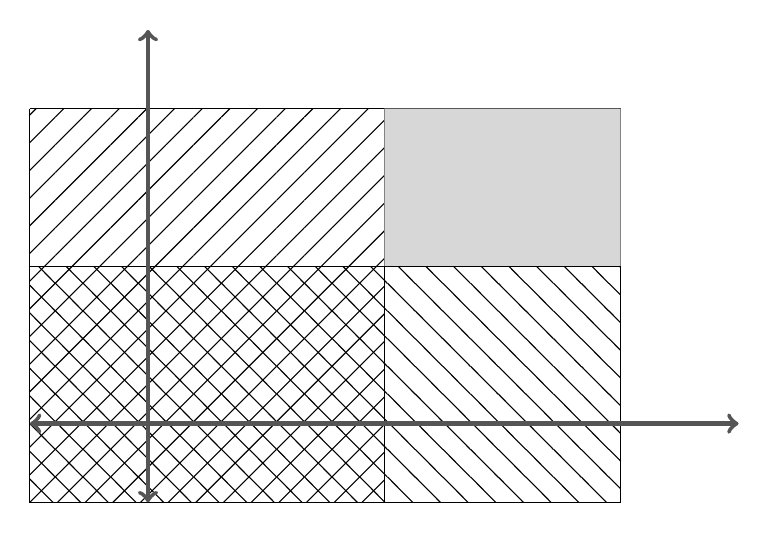
\begin{tikzpicture}[xscale=1.5]
  \coordinate (zzzz) at (-1,-1);
  \coordinate (a1zz) at ( 2,-1);
  \coordinate (zza2) at (-1, 2);
  \coordinate (b1zz) at ( 4,-1);
  \coordinate (zzb2) at (-1, 4);
  \coordinate (b1b2) at ( 4, 4);
  \coordinate (a1b2) at ( 2, 4);
  \coordinate (b1a2) at ( 4, 2);
  \coordinate (a1a2) at ( 2, 2);

  % Boxes
  \draw[] %
    (zzb2) -- (b1b2) -- (b1zz) -- (zzzz) -- (zzb2);
  \draw[pattern=my north west lines, line space=10pt] %
    (zza2) -- (b1a2) -- (b1zz) -- (zzzz) -- (zza2);
  \draw[pattern=my north east lines, line space=10pt] %
    (zzb2) -- (a1b2) -- (a1zz) -- (zzzz) -- (zzb2);
  \draw[color=d4gray, fill=d4gray, opacity=0.5] %
    (a1a2) -- (a1b2) -- (b1b2) -- (b1a2);

  % Axis
  \draw[d4black, ultra thick, <->] (-1,0) -- (5,0);
  \draw[d4black, ultra thick, <->] (0,-1) -- (0,5);
\end{tikzpicture}
\end{figure}
\end{rmk}

\begin{prop}\emph{(From CDF to Probability Measure)}
Let $S$ denote the set of all hypercubes
\begin{align*}
  S = \left\{ (a_1,b_1]\times\cdots\times(a_n,b_n]
  \;|\; a_i\in\bar{\R}, \; b_i\in\R\right\}
\end{align*}
Given a function $F$ satisfying Definition~\ref{defn:F}, define
\begin{align*}
  P\big[\, (a_1,b_1]\times\cdots\times(a_n,b_n] \,\big] :=
  \Delta_{a_1,b_2}
  \cdots
  \Delta_{a_n,b_n}
  F(x_1,\ldots,x_n)
\end{align*}
Then $P$ defines a probability measure on $S$ with a unique extension to
$\sB(\R)^{\otimes n}$.
\end{prop}
\begin{proof}
$S$ forms a semiring, and it is precisely the set that generates the
Borel $\sigma$-algebra $\sB(\R)^{\otimes n}$, Moreover, $P$ is
$\sigma$-finite. So by Caratheodory's Extension Theorem, $P$ defined
above on $S$ has a unique extension to $\sB(\R)^{\otimes n}$.
\end{proof}


\begin{defn}
Let $X:(\Omega,\sF,P)\ra (\R,\sB(\R))$ and $P$ a probability measure,
Then define
\begin{alignat*}{3}
  \E[X] &= \int_\Omega X dP &&\forall X\in L^1\\
  \Var[X] &= \E[(X-\E[X])^2]  &&\forall X\in L^2\\
  \Cov[X,Y] &= \E[(X-\E[X])(Y-\E[Y])] \qquad&&\forall X\in L^2
\end{alignat*}
\end{defn}

\begin{prop}
Given measurable $X\in L^1(\Omega,\sF,P)$ and $P$ a probability measure,
\end{prop}


\subsection{Independence and Borel-Cantelli}

\begin{defn}(Independence)
Let $(\Omega,\sF,P)$ be a probability space and let $J$ be a non-empty
indexing set. We define the following types of independence
\begin{enumerate}
  \item \emph{Events}: A family $\{A_\alpha\}_{\alpha\in J}$ is
    independent if
    \begin{align*}
      P[A_{i_1} \cap \cdots \cap A_{i_m}]
      = P[A_{i_1}]\times \cdots \times P[A_{i_m}]
    \end{align*}
    for every finite sequence of distinct elements
    $\{i_1,\ldots,i_m\}\subseteq J$.

  \item \emph{Family of $\sigma$-algebras}: A family of
    $\sigma$-algebras $\{\sF_\alpha\}_{\alpha\in J}$
    (where each $\sF_\alpha\subseteq \sF$ for all $\alpha\in J$)
    is independent if the family of events
    $\{A_\alpha\}_{\alpha \in J}$ is independent where
    $A_{\alpha}\in \sF_{\alpha}$ $\alpha\in J$.

    In other words, construct the family of events
    $\{A_\alpha\}_{\alpha \in J}$ by plucking out some
    $A_\alpha \in \sF_\alpha\subseteq \sF$ for all $\alpha \in J$. The
    resulting family of events must be independent according to the
    first definition above for the family
    $\{\sF_\alpha\}_{\alpha \in J}$ to be independent.

  \item \emph{Random Variables}: A family of random variables
    $\{X_\alpha\}_{\alpha\in J}$ is independent if
    $\{\sigma(X_\alpha)\}_{\alpha \in J}$ is independent.
\end{enumerate}
\end{defn}

\begin{prop}\emph{(Characterizations of Independence of Random Variables)}
Let $\{X_n\}\nN$ be a sequence of random variables on probability space
$(\Omega,\sF,P)$. Then the following are equivalent
\begin{enumerate}
  \item $X_1,\ldots,X_N$ independent (by the definition above)
  \item For all \textbf{bounded} Borel functions (i.e.
    $f_n:(\R,\sB(\R)) \ra (\R,\sB(\R))$ measurable), we have
    \begin{align*}
      \E\left[\prod\nN f_n(X_n)\right]
      =
      \prod\nN \E\left[f_n(X_n)\right]
    \end{align*}
  \item For any $u\in \R^N$, we have
    \begin{align*}
      \E\left[e^{iu^T X}\right]
      =
      \prod\nN \E\left[e^{iu_n X_n}\right]
    \end{align*}
    where $X := \begin{pmatrix} X_1 &\cdots & X_N \end{pmatrix}'$.
\end{enumerate}
\end{prop}
\begin{cor}
If $X,Y\in L^2$ are independent, then
\begin{align*}
  \E[XY] &= \E[X]\E[Y] \\
  \Corr[X,Y] &= 0
\end{align*}
\end{cor}
\begin{proof}
For fixed $m$, define
\begin{align*}
  X_m := \max\{\min\{X,m\}, -m\}
\end{align*}
For each $m$, the statement should hold. Use Lebesgue's convergence
theorem.
\end{proof}

\begin{defn}(Limsup and Liminf of Events)
Given a sequence of sets $\{A_n\}\ninf$, define the limsup of events
\begin{align*}
  \limsup A_n := \bigcap\ninf \bigcup_{m \geq n} A_m
\end{align*}
If $x\in \limsup A_n$, then for any $N$, there will be an $m>N$ such
that $x\in A_m$. This is like ``$x$ shows up infinitely often.''

Define the liminf of events
\begin{align*}
  \liminf A_n := \bigcup\ninf \bigcap_{m \geq n} A_m
\end{align*}
If $x\in \liminf A_n$, then for some $N$, we will have $x\in A_m$ for
all $m > N$. It shows up in all sets, with only finitely many
exceptions.
\end{defn}

\begin{lem}\emph{(Borel-Cantelli)}
Let $\{A_n\}\ninf$ be a sequence of events in probability space
$(\Omega,\sF,P)$. Then
\begin{align*}
  \sumninf P(A_n) < \infty
  \quad\implies\quad
  P\left(\bigcap\ninf \bigcup_{m\geq n} A_n\right) = 0
\end{align*}
and
\begin{align*}
  \begin{rcases}
    \{A_n\}\ninf \; \text{\emph{independent}}\\
    \sumninf P[A_n] = \infty
  \end{rcases}
  \quad\implies\quad
  P\left(\bigcap\ninf \bigcup_{m\geq n} A_n\right) = 0
\end{align*}
\end{lem}

\clearpage
\subsection{Conditional Probabilities and Expectations}

\subsubsection{Finite Probability Spaces}

\begin{defn}(Decomposition)
Suppose we have a probability space $(\Omega,\sA,P)$. Then a
\emph{decomposition} is any collection
\begin{align*}
  \sD = \{D_1,\ldots,D_N\}
\end{align*}
such that the collection is pairwise disjoint (i.e.\
$D_n\cap D_m=\emptyset$ for all $n\neq m$) and
\begin{align*}
  \Omega = \bigcup\nN D_n
\end{align*}
\end{defn}

\begin{defn}(Atoms of Algebra $\sA$)
Suppose we have an algebra $\sA$. An \emph{atom} is any set $A\in \sA$
such that it's only subsets are $\emptyset$ and $A$.
Atoms are like the prime numbers of an algebra---you can't divide them
up into smaller pieces that are also in the algebra.

Any arbitrary $B\in\sA$ can be expressed as a union of atoms. Moreover,
you can always create a decomposition of the sample space $\Omega$ into
the set of all atoms, since atoms are pairwise disjoint (see next
proposition).
\end{defn}

\begin{rmk}
Shiryaev refers to elements of any arbitrary decomposition as ``atoms.''
I do not. I reserve that term for sets strictly satisfying the
definition above.

Though the set of all atoms \emph{always} forms a decomposition, by my
terminology, you can have a decomposition of $\Omega$ consisting of sets
that are not atoms.
\end{rmk}

\begin{prop}
Any two atoms of an algebra are disjoint.
\end{prop}
\begin{proof}
Suppose that $A,B\in\sA$ are two distinct atoms. Since $\sA$ is an
algebra, then $A\cap B\in\sA$. If this intersection were nonempty, it
would violate the definition of $A$ and $B$ as atoms.
\end{proof}


\begin{ex}
Let $\{x_1,\ldots,x_N\}$ denote the range of random variable $X$ defined
on probability space $(\Omega,\sA,P)$. Then the sets
\begin{align}
  \{X=x_1\}\quad\cdots\quad\{X=x_N\}
  \label{atoms}
\end{align}
form a decomposition of $\Omega$. Moreover, Collection~\ref{atoms}
is also the collection of all atoms of $\alpha(X)$, the algebra
generated by $X$ (i.e.\ the algebra generated by Collection~\ref{atoms}).
\end{ex}


\begin{defn}(Bayes Rule: Conditional Probability Given an Event)
\label{defn:bayesrule}
The conditional probability of event $A$ ocurring given $B$ occurring
(assuming $P(B)>0$) is
\begin{align*}
  P[A|B] = \frac{P[A\cap B]}{P[B]}
\end{align*}
\end{defn}

\begin{defn}(Conditional Probability Given a Decomposition)
Let $\sD$ be a decomposition of sample space $\Omega$. Then
the \emph{conditional probability with respect to decomposition $\sD$}
denoted $P[A|\sD]$ is a random variable defined
\begin{align*}
  P[A|\sD](\omega) = \sumnN P[A|D_n] I_{D_n}(\omega)
\end{align*}
Since a decomposition consists of pairwise disjoint sets, $\omega$ is in
\emph{some} $D_i\in\sD$. The random variable $P[A|\sD](\omega)$ takes
$\omega$, finds that $D_i$, and returns $P[A|D_i]$ as defined in Bayes
Rule, Definition~\ref{defn:bayesrule}.
\end{defn}

We see here how a decomposition can represent our ``information.''
Suppose we have an event $A$. We have some baseline probability of it
occurring, $P[A]$. The conditional probability $P[A|\sD](\omega)$ is a
function that tells us a new ``updated'' probability for $A$ occuring
given that $\omega$ occurred. Let's consider a few examples for $\sD$.

Say that $\sD_1=\{\Omega\}$. This is a very coarse decomposition.
Moreover, by the definition, it's clear that
\begin{align*}
  P[A|\sD_1](\omega)=P[A|\Omega]=P[A]
  \qquad\forall\omega\in\Omega
\end{align*}
Here we see that $\sD_1$ represents a decomposition without much
information.  Knowing which $\omega$ turns up does not cause us to
revise our baseline probability $P[A]$. That's in sharp contrast to the
next example.

Suppose that we have a decomposition $\sD_2=\{A,A^c\}$. Then by the
definition
\begin{align*}
  P[A|\sD_2](\omega)
  =
  \begin{cases}
    1 & \omega \in A \\
    0 & \omega \in A^c \\
  \end{cases}
\end{align*}
The decomposition $\sD$ conveys a lot of information about event $A$.

More generally, conditional probabilities relative to events like
$P[A|B]$ are like ``I tell you $B$ happened. You tell me
the probability $A$ happened too.'' On the other hand, conditional
probabilities relative to decompositions are like ``I tell you $\omega$
happened and give you a collection of probabilities
$\{P[A|D_n]\}_{D_n\in\sD}$. You then look up the $D_i$ such that
$\omega\in D_i$ and tell me $P[A|D_i]$.'' It's more general because it's
a function mapping from the sample space to numbers, and that mapping
depends crucially on $\sD$.

\begin{defn}(Conditional Expectation with Respect to an Algebra)
Let $\sA$ be an algebra with atoms $A_1,\ldots,A_m$. The conditional
expectation of $X$ with respect to $\sA$ is the random variable
\begin{align*}
  \E[X|\sA](\omega)
  &=
\end{align*}
\end{defn}

\begin{defn}(Law of Total Probability)
Given a decomposition $\sD=\{D_1,\ldots,D_N\}$ of $\Omega$,
it's clear for $B\subseteq\Omega$ that
\begin{align*}
  B = \bigcup\nN (B\cap D_n)
\end{align*}
Therefore, we get the law of total probability
\begin{align*}
  P[B] = \sumnN P[B|D_n]P[D_n]
\end{align*}
\end{defn}

\subsubsection{General Probability Spaces}

\begin{prop}
\end{prop}


\subsection{Gaussian Processes}

\begin{defn}
(Symmetric Positive Semi-definite and Positive Definite Functions)
Given indexing set $J$, the function $C:J^2 \ra \R$ where we define
$c_{st}:=c(s,t)$ is
\begin{enumerate}
  \item \emph{Symmetric}: $c_{st}=c_{ts}$ for all $s,t \in J$.
  \item \emph{Positive (Semi-)definite}: The matrix
    \begin{align*}
      (c_{t_i,t_j})^d_{i,j=1}
      &=
      \begin{pmatrix}
        c_{t_1,t_1} &\cdots & c_{t_1,t_d} \\
        \vdots &\ddots & \vdots \\
        c_{t_d,t_1} &\cdots & c_{t_d,t_d} \\
      \end{pmatrix}
      \in \R^{d\times d}
    \end{align*}
    is positive (semi-)definite for every finite sequence
    $\{t_1,\ldots,t_d\}$ of different elements of $J$.
\end{enumerate}
\end{defn}

\begin{rmk}
Any inner product in a Hilbert Space is positive semi-definite. So
rather than take a function $C$, fix a sequence
$\{i_1,\ldots,i_d\}\subseteq J$, and check the resulting matrix for
positive (semi)definiteness, just see if it's an inner product in a
Hilbert space.
\end{rmk}


\subsection{Martingale Theory}





\clearpage
\section{Transformation Theory}

Throughout this subsection, we'll only consider continuous random
variables. So let's start with $n$ random variables, $X_1, \ldots, X_n$,
(not necessarily iid) which have jdf
   \[ f_{X_1, \ldots, X_n}(x_1, \ldots, x_n) \]
Now let's suppose that we define a new random variable $Y$, which is
some function
   \[ Y = g(X_1, \ldots, X_n) \]
Let's review some reasons why we might want to construct such a $Y$:
\begin{enumerate}
  \item We might want to build up a more complex random variable $Y$
    by transforming relatively simple ones.
  \item Often, a maximum likelihood estimator for some parameter will be
    a function of random variables $X_i$.
  \item Many test statistics are, in fact, \emph{derived} statistics
    dependent on the variables $X_i$.
\end{enumerate}
So we'll need to be able to say something about the distribution of $Y$.
We'll start with the univariate case where $n=1$, so that $Y=g(X)$. From
there, we'll move onto the multivariate case.

\subsection{Univariate Case}

Throughout this section, we'll assume that $X$ has a known density
function, $f_X(x)$. For some differentiable function $g$, we then define
$Y = g(X)$. The goal is to find $f_Y(y)$.

\begin{thm}\emph{(Monotonic Transformations)}
Suppose that $g$ is a monotonic function. Then
\begin{align*}
   f_Y(y) &= \left[f_X(x) \left\lvert \frac{dx}{dy}\right\rvert
      \right]_{x = g^{-1}(y)} \\
    &= \left[ f_X(x) \left\lvert \frac{dy}{dx}\right\rvert^{-1}
      \right]_{x = g^{-1}(y)}
\end{align*}
\end{thm}

\begin{thm}\emph{(Non-Monotonic Transformations)}
Suppose $g$ is some non-monotonic function. Then split up the function
into monotonic segments. Suppose that there are $n$ such monotonic
segments of $g$, denoted $g_1,\ldots,g_n$. Then
\begin{align}
   \label{nonmontrans}
   f_Y(y)
   &= \sumin \left[ f_X(x_i) \left\lvert \frac{dx_i}{dy}
      \right\rvert \right]_{x_i=g_i^{-1}(y)}\\
   &= \sumin \left[ f_X(x_i) \left\lvert \frac{dy}{dx_i}
    \right\rvert^{-1} \right]_{x_i=g_i^{-1}(y)}
    \notag
\end{align}
\end{thm}


\subsection{Multivariate Case}

Suppose that we have
$X:=\begin{pmatrix}X_1 & \cdots & X_n\end{pmatrix}'$ with jdf
$f_{X}(x)$.
Now suppose that we have an invertible function $g:\Rn\ra\Rn$. The
invertibility assumption is similar to the monotonicity assumption in
the univariate case.  Let
\begin{align*}
  Y:= \begin{pmatrix} Y_1 \\ \vdots \\ Y_n \end{pmatrix}
  = g(X)
\end{align*}
We can compute the jdf for vector $Y$ as
\begin{align*}
  f_{Y}(y)
  %&= \left[ f_{X}(x) \lvert J \rvert \right]_{x=g^{-1}(y)} \\
   &= \left[
      f_{X}(x)\frac{1}{\lvert J\rvert}
      \right]_{x=g^{-1}(y)}
\end{align*}
where $|J|$ is the determinants of the Jacobian matrix
\begin{equation}
   %J = \begin{bmatrix} \frac{\partial x_1}{\partial y_1} &
      %\frac{\partial x_1}{\partial y_2} & \cdots &
      %\frac{\partial x_1}{\partial y_n} \\
      %\vdots & & \ddots & \vdots \\
      %\frac{\partial x_n}{\partial y_1} &
      %\frac{\partial x_n}{\partial y_2} & \cdots &
      %\frac{\partial x_n}{\partial y_n}
   %\end{bmatrix} \qquad \qquad
   J = \begin{bmatrix} \frac{\partial g_1}{\partial x_1} &
      \frac{\partial g_1}{\partial x_2} & \cdots &
      \frac{\partial g_1}{\partial x_n} \\
      \vdots & & \ddots & \vdots \\
      \frac{\partial g_n}{\partial x_1} &
      \frac{\partial g_n}{\partial x_2} & \cdots &
      \frac{\partial g_n}{\partial x_n}
   \end{bmatrix}
\end{equation}
where $\frac{\partial g_i}{\partial x_j}$ is the partial derivative of
the $i$th element of $g(X)$ with respect to the $j$th element of vector
$X$.

Often, we will even use this to do transformations that are not
1-to-1. That will involve doing a transformation that \emph{is}
1-to-1 using this method with dummy variables, then integrating
out those dummy variables.


\clearpage
\section{Select Probability Distributions}


\subsection{Multivariate Normal}

The univariate normal distribution is an extremely familiar concept
where some random variable $X$ can take values along the real with
probabilities that match the famouse bell-curve. Recall the probability
density function of
   \[ f_Y(y) = \frac{1}{\sigma \sqrt{2\pi}} \; e^{-\frac{1}{2\sigma^2}
      (y - \mu)^2} \]
However, that's limited to only one dimension, and we would like to
generalize to higher dimensions. In the next-simplest 2-dimensional
case, we'd like a distribution that actually looks like a bell---where
potentional values can range over the real plane, $\mathbb{R}^2$, with
the density clustered around some mean before tapering off in all
directions, as below.
\begin{figure}[h!]
   \centering
   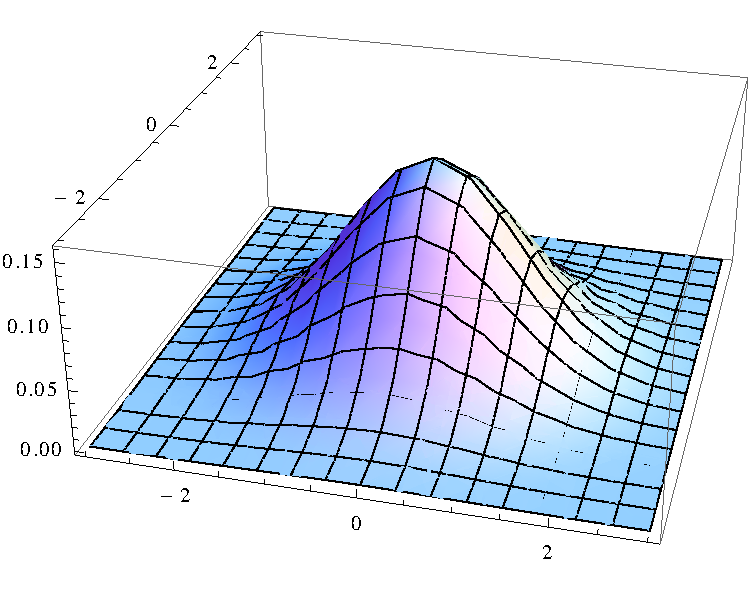
\includegraphics[scale=0.40]{multivariate.pdf}
\end{figure}
\\
This figure has mean zero for both $X_1$ and and $X_2$, and
which are independent, implying $\sigma = I_2$, the identity matrix.
It's easy to see that any vertical cuts parallel to $xz$ or $yz$ planes
will yield a traditional normal random variable. This of course
generalizes to higher dimensions, although we can't display it so nicely.
\\
\\
This generalization will give us the
\emph{Multivariate Normal (MVN) Distribution}.
This turns out to be an extremely useful distribution. Let's highlight
a few applications here:
\begin{enumerate}
  \item The MVN distribution has applications in Bayesian multivariate
    regressions (i.e. Bayesian regressions with more than one
    ``independent,'' ``predictor,'' or ``$X$'' variable).  In such
    applications, we hope to find the posterior distribution of the
    $\beta$ regression vector, and it's common to assume a MVN prior on
    $\beta$ that results in an MVN posterior for $p(\beta|y)$.

  \item Next, we often use the MVN distribution to describe
    \emph{recurrence relations}, where we try to forecast an MVN RV one
    period into the future, given current information about the RV, like
    it's current value and distribution. One example would include
    jointly forecasting height \emph{and} weight in the future given
    current height and weight.

  \item Finally, the MVN distribution forms the basis for VARs, which
    are used to forecast different economic variables one period into
    the future, expressing each future variable as a function of lags of
    itself and other economic variables.  However, VARs are too broad
    and interesting a subject to elicit only a cursory summary in this
    note.  I'll write a more extensive summary of them elsewhere.
\end{enumerate}

In this note, the multivariate distribution will apply to a
$d$-dimensional random vector
\[ X = \begin{pmatrix} X^{(1)} & X^{(2)} & \ldots & X^{(d)} \end{pmatrix}^T,
    \qquad X  \sim N_d(\mu, \Sigma) \]
where $\mu$ is the $n$-dimensional \emph{mean vector},
\[ \mu = \begin{pmatrix} EX^{(1)} & EX^{(2)} & \ldots & EX^{(d)} \end{pmatrix}^T,
      \]
and where $\Sigma$ is the $d\times d$ \emph{covariance matrix}, which
is defined and has in its $i,j$ entry
\[ \sigma^2 = E\left[ (X - \mu) (X-\mu)^T\right] \in
   \mathbb{R}^{N\times N} \]
\[ \Sigma_{ij} = Cov(X^{(i)}, X^{(j)}), \qquad i,j = 1, \ldots, d\]
Superscripts with parentheses, like ``$X^{(i)}$,'' will denote
$i$th element of the MVN RV ``$X$,'' while ``$X_t$'' will denote
an MVN RV at time $t$.


\begin{defn}(Multivariate Normal)
A random vector $X$ has a \emph{multivariate normal}
distribution if every linear combination of its components,
\[ Y = a_1 X^{(1)} + \ldots + a_d X^{(d)} \]
\[ \Leftrightarrow Y = {a} X, \qquad
    {a} \in \mathbb{R}^{d} \]
is \emph{univariate normally
distributed}, with a corresponding mean and variance. This gives a
joint density function of
\begin{equation}
    \label{pdf2}
    f_{X}({x}) = \frac{1}{(2\pi)^{d/2}\lvert \Sigma \rvert^{1/2}}
	\; e^{ -\frac{1}{2} ({x} - \mu)^T \;
	\Sigma^{-1} ({x} - \mu) }, \qquad \lvert\Sigma\rvert =
      \det\Sigma \qquad x \in \mathbb{R}^d
\end{equation}
Note, we impose the requirement that $\Sigma$ is symmetric and positive
definite.  Symmetric because the correlation of $X$ and $Y$ equals the
correlation of $Y$ and $X$.
\end{defn}
{\sl Terminology}: I'll often us MVN to refer to the case where $X$ is
a vector with $d\geq2$; however, it should be clear that the univariate
normal distribution is just a special case where $d=1$. Therefore,
when speaking about an RV that could be either MVN or univariate normal
\emph{or} properties that apply equally well to either
type of RV, I'll often use the term \emph{Gaussian}
both for convenience and out of reverence to long-dead German-speaking
mathematicians. Stimmt?


It's fairly common to consider linear transformations and functions
of a multivariate normally distributed random variable.  For instance,
we might have an economic or statistical model with a recurrence
relation to describe the dynamics of some process:
\[ X_{t+1} = A X_{t} + {V}_{t} \]
where ${V}_t$ is some innovation or random noise vector.
Therefore, it would be useful to be able to derive the distributions
of \emph{functions} or \emph{linear transformation} of multivariate
normal random variables.

So let's find the probability distribution of a linear transforamtion
of an MVN RV. Begin by assuming
\begin{align*}
    X &= A{Y}, \qquad {Y} \sim
	\text{MVN}(\mu, \Sigma) \\
    \Rightarrow \quad f(y) &= k \; \exp\left\{-\frac{1}{2} (y - \mu)^T
	\; \Sigma^{-1} (y-\mu)\right\}
\end{align*}
where $k$ is a constant.\footnote{The constant will come from the
definition of the distribution given above in Equation \ref{pdf}, but
it's boring algebra not that interesting, so I'll suppress the details.}
Assuming that $A$ is invertible, we substitute in, using Equation
, to get the distribution of $X$:
\begin{align}
    \label{midway}
    \Rightarrow \quad f_X(A^{-1}x) &= k' \exp\left\{-\frac{1}{2} (A^{-1}x - \mu)^T
	\Sigma^{-1} (A^{-1}x-\mu)\right\}
\end{align}
Next, since the expectation is a linear operator, we can use the fact
that
\begin{align*}
    EX &= E[A{Y}] = A E{Y} = A \mu \\
    \Rightarrow \quad \mu_* &= A \mu \\
    \Leftrightarrow \quad \mu &= A^{-1} \mu_*
\end{align*}
where $\mu'$ is the mean vector of $X$.  With that, we
can substitute back into Equation \ref{midway} and simplify even
further, using convenient matrix manipulations like the distributivity
property, associativity, etc.:
\begin{align*}
    f_X(A^{-1}x) &= k' \exp\left\{-\frac{1}{2} (A^{-1}x - \mu)^T \;
	\Sigma^{-1} (A^{-1}x-\mu)\right\} \\
    &= k' \exp\left\{-\frac{1}{2} (A^{-1}x - A^{-1}\mu_*)^T \;
	\Sigma^{-1} (A^{-1}x-A^{-1}\mu_*)\right\} \\
    &= k' \exp\left\{-\frac{1}{2} [A^{-1}(x - \mu_*)]^T \;
	\Sigma^{-1} [A^{-1}(x-\mu_*)]\right\} \\
    &= k' \exp\left\{-\frac{1}{2} (x - \mu_*)^T \; [(A^{-1})^T \;
	\Sigma^{-1} A^{-1}] (x-\mu_*)\right\} \\
    &= k' \exp\left\{-\frac{1}{2} (x - \mu_*)^T \;
	\Sigma_*^{-1} \; (x-\mu_*)\right\} \\
    \Rightarrow X &\sim  \text{MVN}(\mu_*, \Sigma_*),
    \qquad \text{where $\mu_* = A\mu$ and $\Sigma_* = A\Sigma A^T $}
\end{align*}
This is huge! It means \emph{linear transformations of MVN
RV's are themselves MVN.}


If you're familiar with the standard univariate normal RV,
then you can probably guess what the standard MVN RV is:
\begin{equation}
    {Z} \sim \text{MVN}(0, \; I_d)
\end{equation}
where $I_d$ is the $d\times d$ identity matrix.  This form for
the covariance matrix also suggests that the different components
of ${Z}$ (denoted $Z_1, Z_2, \ldots, Z_d$) are independent and
Gaussian.
\\
\\
Moreover, just like we can build from a standard univariate to
a general univariate.  To do so, we'll use the results from the
last section, since building from a standard MVN
to general MVN simply involves linear transformations of the components.
Specifically, we can express the MVN RV ${X}$ as follows
\begin{equation}
    {X} = \mu + A{Z}, \qquad {X}\sim
	\text{MVN}(\mu, AA^T)
\end{equation}
{\sl Computation}: Suppose we know that we want ${X}$ to
be MVN($\mu, \; \Sigma)$, and we can only generate ${Z}$.
How do we choose $A$ such that $AA^T = \Sigma$.  Typically, we'll
have to use something like a \emph{Cholesky Factorization}
algorithm to find the correct $A$ in the form of a lower triangular
matrix. And if $\Sigma$ is symmetric, positive definite, then
$A$ is guaranteed to exist and this approach will work.
The algorithm itself can be found in the appendix.


So to summarize, MVN (or Gaussian) RV's are particularly nice to work with because
of some convenient properties:
\begin{enumerate}
    \item Suppose that ${X}$ and ${Y}$ are \emph{univariate}
	normally distributed and independent. This then implies that they are
	\emph{jointly normally distributed}. In other words,
	$\begin{pmatrix} {X} & {Y} \end{pmatrix}$ must have a multivariate
	normal distribution.
    \item Linear functions of Gaussians are Gaussian. So if $A$
	is a constant matrix and ${X}$ is MVN, then $A{X}$
	is also MVN.
    \item Uncorrelated Gaussian random variables are independent.
    \item Conditions Gaussian's are normal. So if $X_1$ and $X_2$
	are two components of a MVN RV, ${X}$, then
	$X_1 | X_2$ is normal, and vice versa.
\end{enumerate}

\clearpage
\subsection{$\Chi^2$ Distribution}


\begin{defn}
The $\Chi^2_\nu$ distribution with $\nu$ degrees of freedom is the sum of
$\nu$ squared standard normal random variables:
\begin{align*}
  Y \sim \Chi^2_\nu
  \quad\implies\quad
	 Y = \sum^\nu_{i=1} Z^2_i
   \qquad Z_i \sim N(0,1)
\end{align*}
\end{defn}

\begin{prop}
\label{prop:chisum}
Given $Y_i \sim \Chi_{\nu_i}^2$, then
\begin{align*}
  \sum^n_{i=1} Y_i \sim \Chi^2_{\nu}
  \qquad
  \text{where}\;
  \nu=\sum^n_{i=1} \nu_i
\end{align*}
In words, sums of $\Chi^2$ RVs are also $\Chi^2$ distributed.
\end{prop}

\begin{cor}
\label{cor:chimu}
Suppose that $Y_i \sim N(\mu,\sigma^2)$. Then
\begin{align*}
  \sum^n_{i=1} \frac{(Y_i-\mu)^2}{\sigma^2}  \sim \chi^2_n
\end{align*}
\end{cor}

\begin{cor}
Suppose that $Y_i \sim N(\mu,\sigma^2)$. Then
\begin{align*}
  \sum^n_{i=1} \frac{(Y_i-\bar{Y})^2}{\sigma^2}  \sim \Chi^2_{n-1}
\end{align*}
In other words, if we estimate the mean by the sample average $\bar{Y}$,
we loose one degree of freedom.
\end{cor}
\begin{proof}
Start first with the sum assuming we have the true mean $\mu$. We'll
break it up
\begin{align*}
	 \sum^n_{i=1} \frac{(Y_i-\mu)^2}{\sigma^2} &= \frac{1}{
	    \sigma^2} \sum^n_{i=1} (Y_i - \bar{Y}+ \bar{Y}-\mu)^2 \\
	    &= \frac{1}{\sigma^2} \sum^n_{i=1}  (Y_i - \bar{Y})^2
	    + \frac{2}{\sigma^2} \sum^n_{i=1} (Y_i-\bar{Y})(\bar{Y}-\mu)
	    + \frac{1}{\sigma^2} \sum^n_{i=1} (\bar{Y}-\mu)^2
      %\\
			%&= \frac{1}{\sigma^2} \sum^n_{i=1}  (Y_i - \bar{Y})^2
			%+ \frac{2(\bar{Y}-\mu)}{\sigma^2} \sum^n_{i=1} (Y_i-\bar{Y})
			%+ \frac{n(\bar{Y}-\mu)^2 }{\sigma^2}  \\
\end{align*}
If you do out the algebra, the middle term is zero and drops out, so we
are left with
\begin{align*}
	 \sum^n_{i=1} \frac{(Y_i-\mu)^2}{\sigma^2}
	 &= \sum^n_{i=1}\frac{(Y_i - \bar{Y})^2 }{\sigma^2} +
	    \left(\frac{\bar{Y}-\mu }{\sigma /\sqrt{n}}\right)^2
\end{align*}
The LHS is $\Chi^2_n$ by Corollary~\ref{cor:chimu}.
On the RHS, the second term is the mean estimator divided by the
standard error of the mean; therefore, that term in parentheses is a
$N(0,1)$ random variable. When squared, the result is a $\Chi_1^2$
random variable. Taking that over to the LHS and applying
Proposition~\ref{prop:chisum}, we conclude that
\begin{align*}
  \sum^n_{i=1}\frac{(Y_i - \bar{Y})^2}{\sigma^2}
  \sim \Chi^2_{n-1}
\end{align*}
\end{proof}
\begin{rmk}
This result is extremely important for deriving the distribution of
different estimators, variance estimators in particular.
\end{rmk}

\begin{prop}
Suppose that $Y$ has a $\Chi^2$ distribution with $\nu$ degrees of
freedom. Then the distribution is a special case of the gamma
distribution, where $\alpha = \nu/2$ and $\beta = 1/2$ with the pdf and
descriptive statistics
\begin{equation}
   f_Y(y) = \frac{1}{2^{\frac{\nu}{2}} \Gamma\left(\frac{\nu}{2}\right)}
      x^{\frac{\nu}{2} - 1} e^{-\frac{x}{2}} \qquad
\text{Mean} = \nu, \qquad \text{Variance} = 2 \nu
\end{equation}
\end{prop}
\begin{proof}
Since we can generate a $\Chi^2(\nu)$ random variable by summing the
square of $\nu$ independent N(0,1) random variables, this suggests that
we can use an induction argument to get the distribution.
\end{proof}

\subsection{Student's t-Distribution}

\begin{defn}
Let $Z\sim N(0,1)$ and $Y\sim \Chi^2_n$ be independent random variables.
Then
\begin{align*}
  X = \frac{Z}{(Y/n)^{1/2}}
  \sim t_n
\end{align*}
where $n$ is the degrees of freedom.
\end{defn}
%In order to generate a variable that has $t$ distribution with
%$n-1$ degrees of freedom,
%we start by supposing that $Y_i\sim \text{NID}(\mu,\sigma^2)$. From
%there, we define
%\begin{align*}
   %\bar{Y} = \frac{1}{n} \sum^n_{i=1} Y_i \qquad
   %S^2 &= \frac{1}{n-1} \sum^n_{i=1} (Y_i - \bar{Y})^2 \\
   %&=\frac{1}{n-1} \left( Y_1^2 + \cdots + Y_n^2 - n \bar{Y}^2\right)
%\end{align*}
%The statistics $\bar{Y}$ and $S^2$ are useful because they are both
%unbiased estimators of $\mu$ and $\sigma^2$, respectively.
%And before we get to the derivation, we make one final note:
%\emph{Cochran's Theorem}
%says that $\bar{Y}$ and $S^2$ are independent for the normal
%distribution.\footnote{This holds for \emph{no} other distributions;
%it is unique to the normal.}
%\\
%\\
%Now let's define the statistic, $T$,
%whose distribution we hope to find:
   %\[ T = \frac{\bar{Y}-\mu}{S/\sqrt{n}} \qquad Y_i \sim \text{NID}(\mu,
      %\sigma^2) \]
%But after a bit of rearranging and variable definitions, we get
%\begin{align*}
   %T &= \frac{(\bar{Y}-\mu)\sqrt{n} }{S} = \frac{
      %\frac{\bar{Y}-\mu}{\sigma/\sqrt{n}}}{\sqrt{\frac{S^2}{\sigma^2}
      %\cdot \frac{n-1}{n-1}}} \\
      %&= \frac{W_1}{\sqrt{W_2 / (n-1)}}
%\end{align*}
%Now it's clear by how we defined $W_1$ and $W_2$ that $W_1$ has a
%N(0,1) distribution, while $W_2$ has a $\chi^2$ distribution with
%$n-1$ degrees of freedom. Since $W_1$ and $W_2$ are \emph{independent}
%by Cochran's theorem, the jdf of $W_1, W_2$ is
   %\[ f_{W_1, W_2}(w_1, w_2) = \left(
      %\frac{1}{\sqrt{2\pi}} \; e^{-\frac{1}{2} w_1^2}\right)\left(
      %\frac{1}{ 2^{\frac{n-1}{2}} \Gamma\left(\frac{n-1}{2}\right)}
      %\; w_2^{\frac{n-1}{2} -1} e^{-\frac{1}{2}
      %w_2}\right)
      %\]
%Now we just hope to find the jdf of $T$. Since transformations must be
%1-to-1 in the number of variables, we'll choose
%a dummy variable, $V$, and define to simplify the mess of fractions
%in the jdf:
%\[ V =W_2, \qquad k = \frac{1}{\sqrt{2\pi}} \cdot \frac{1}{
   %2^{\frac{n-1}{2}} \Gamma\left(\frac{n-1}{2}\right)} \]
%This leads us to from the Jacobian matrix to go from $W_1$ and
%$W_2$ to $T$ and $V$:
%\[ J^* = \det \begin{bmatrix} \frac{\partial T}{\partial W_1} &
   %\frac{\partial T}{\partial W_2} \\
   %\frac{\partial V}{\partial W_1} &
   %\frac{\partial V}{\partial W_2} \end{bmatrix} =
   %\begin{vmatrix} \frac{1}{\sqrt{W_2/(n-1)}} && \frac{\partial T}{
      %\partial W_2} \\ 0 && 1
   %\end{vmatrix} = \frac{1}{\sqrt{W_2/(n-1)}}
   %\]
%Now we can get the jdf of $T$ and $V$:
%\begin{align*}
   %f_{T,V}(t,v) &= \left[ f_{W_1,W_2}(w_1, w_2) \cdot
      %\lvert J^* \rvert^{-1}
      %\right]^{w_1 = g_1^{-1}(t,v)}_{w_2 = g_2^{-1}(t,v)}\\
   %&= \left[ k \cdot e^{-\frac{1}{2} w_1^2}
      %w_2^{\frac{n-1}{2} - 1} e^{-\frac{1}{2} w_2}  \left(
      %\frac{1}{\sqrt{w_2/(n-1)}}\right)^{-1}
      %\right]^{w_1 = t \sqrt{\frac{v}{
      %n-1}}}_{w_2=v}\\
      %&= \frac{k}{\sqrt{n-1}} v^{\frac{n-1}{2} - \frac{1}{2}}
      %e^{-\frac{1}{2} v\left( 1 + \frac{t^2}{n-1}\right)}
%\end{align*}
%Now we just need to integrate out the dummy variable, $V$, to
%get the distribution of $T$, which will require some substitution:
%\[ y = \frac{1}{2} v \left( 1 + \frac{t^2}{n-1} \right), \qquad
   %dv = \frac{2}{\left( 1 + \frac{t^2}{n-1} \right)} \; dy \]
%\begin{align*}
   %\Rightarrow f_{T}(t) &=\frac{k}{\sqrt{n-1}} \int^\infty_0
      %v^{\frac{n-1}{2} - \frac{1}{2}}
      %e^{-\frac{1}{2} v\left( 1 + \frac{t^2}{n-1}\right)} \; dv \\
      %&= \frac{k}{\sqrt{n-1}} \left( \frac{2}{ 1 + \frac{t^2}{n-1} }
      %\right)^{\frac{n-1}{2} + \frac{1}{2}} \int^\infty_0
      %y^{\frac{n-1}{2} - \frac{1}{2}} e^{-y} \; dy
%\end{align*}
%Now we recognize the integral as the $\Gamma(n/2)$ function, so
%we can substitute that in and substitute in for $k$ to get
%\begin{align*}
   %\Rightarrow f_{T}(t) &=\frac{\Gamma(n/2)}{
      %\Gamma\left(\frac{n-1}{2}\right)\sqrt{\pi(n-1)}}
      %\left( 1 + \frac{t^2}{n-1}\right)^{-\frac{n}{2}}
%\end{align*}
%So for a given $n$, this is the $t$-distribution with $n-1$ degrees
%of freedom.
%\\
%\\
%Equivalently, we can also express the distribution in an equally
%common formulation, where the statistic has $\nu$ degrees of freedom:
%\begin{align*}
   %\Rightarrow f_{T}(t) &=\frac{\Gamma\left(\frac{\nu+1}{2}\right)}{
      %\Gamma\left(\frac{\nu}{2}\right)\sqrt{\nu\pi}}
      %\left( 1 + \frac{t^2}{\nu}\right)^{-\frac{\nu+1}{2}}
%\end{align*}

\newpage
\subsection{F-Statistic and Distribution}


\begin{defn}
Closely related to the $t$-distribution (and just as important), we now
want to find the distribution of the $F$-statistic, defined as
\begin{align*}
  Y = \frac{ X_a / a}{X_b / b},\qquad\qquad
  X_a \sim \Chi^2_a
  \quad X_b \sim \Chi^2_b
\end{align*}
Then $Y\sim F_{a,b}$.
\end{defn}
%Since $X_a$ and $X_b$ are assumed independent,
%we can form the jdf as the product of the two density functions
%\begin{align*}
   %f_{X_a, X_b}(x_a, x_b) &= \left(\frac{1}{2^{a/2} \Gamma(a/2)}
      %\; x_a^{a/2 -1} e^{-x_a/2 }\right) \left(
      %\frac{1}{2^{b/2}  \Gamma(b/2)} \;
      %x_b^{b/2 -1} e^{- x_b /2} \right)\\
   %&= k \; x_a^{a/2 -1} \; x_b^{b/2 -1} e^{-\frac{1}{2}(x_a + x_b)} \\
   %\text{where } \quad k &= \frac{1}{ 2^{\frac{a+b}{2}} \Gamma(a/2)
      %\Gamma(b/2)}
%\end{align*}
%Now we want to find the jdf of $F$ and our chosen dummy variable,
%$G=X_b$. To do so, we start with the inverse functions and
%then form the Jacobian matrix:
   %\[ X_a = \frac{a FG}{b}, \qquad X_b = G, \quad\Rightarrow \quad
     %|J| = \begin{vmatrix} \frac{\partial X_a}{\partial F} &
      %\frac{\partial X_a}{\partial G} \\
      %\frac{\partial X_b}{\partial F} &
      %\frac{\partial X_b}{\partial G} \end{vmatrix} =
      %\begin{vmatrix}
	 %\frac{a G}{b} & \frac{a F}{b} \\ 0 & 1
      %\end{vmatrix}
      %= \frac{a}{b} G
      %\]
%This allows us to write the trnasformed jdf
%\begin{align*}
   %p_{F,G}(f,g) &= \left[
      %k x_a^{a/2 -1} x_b^{b/2 -1} e^{-\frac{1}{2}(x_a + x_b)}
      %\left( \frac{a}{b} g\right) \right]^{x_a = a f g/b}_{x_b = g}\\
   %&= k' f^{a/2 -1} g^{\frac{a+b}{2}-1} e^{-\frac{g}{2}\left(
      %\frac{a}{b}f +1 \right)} \\
   %\text{ Where} \qquad k' &= \frac{1}{ 2^{\frac{a+b}{2}} \Gamma(a/2)
      %\Gamma(b/2)} \left( \frac{a}{b}\right)^{\frac{a}{2}}
%\end{align*}
%To get the density function of $F$, we integrate out the dummy
%variable, $G=X_b$, which is a simple $\chi^2$ variable whose support
%is the positive real line:
%\begin{align*}
   %p_F(f) &= k' f^{a/2 -1} \int^\infty_0
      %g^{\frac{a+b}{2}-1} e^{-\frac{g}{2}\left(
      %\frac{a}{b}f +1 \right)} \; dg
%\end{align*}
%We'll make the substitution
   %\[ u = \frac{g}{2}\left(\frac{a}{b} f +1\right) , \qquad
      %g = 2u \left( \frac{a}{b} f +1\right)^{-1} \]
   %\[ dg = 2 \left( \frac{a}{b} f +1\right)^{-1} \; du
      %\]
%\begin{align*}
   %\Rightarrow \qquad p_F(f) &= k' f^{a/2 -1}  \left[
      %2 \left( \frac{a}{b} f +1\right)^{-1}\right]^{\frac{a+b}{2}}
     %\int^\infty_0 u^{\frac{a+b}{2} - 1}
     %e^{-u} \; du
%\end{align*}
%Finally,
%we recognize that the integral is simply the $\Gamma( (a+b)/2)$
%function. This allows us to simplify $p_F$ and substitute back for
%$k'$ to get
%\begin{align*}
   %p_F(f) &= k' f^{a/2 -1}  \left[
      %2 \left( \frac{a}{b} f +1\right)^{-1}\right]^{\frac{a+b}{2}}
      %\Gamma\left(\frac{a+b}{2}\right) \\
   %\Rightarrow \qquad
   %p_F(f) &= \frac{\Gamma\left(\frac{a+b}{2}\right)}{ \Gamma(a/2)
      %\Gamma(b/2)} \left( \frac{a}{b}\right)^{\frac{a}{2}}
      %f^{\frac{a}{2} -1} \left[
	 %1 + \frac{a}{b} f \right]^{-\frac{a+b}{2}}
%\end{align*}
%which is the density function for $F$.



\clearpage
\subsection{Beta Distribution}

One particularly useful random variable is the Beta Distribution, which
model proportions relatively well, as it only takes values between
$0$ and $1$, and which also retains the uniform distribution as a special
case.

A random variable $Y$ has a \emph{beta probability distribution} if
and only if it has density function
\begin{equation}
   \label{pdf}
   f_Y(y) = \begin{cases} \frac{y^{\alpha -1} (1-y)^{\beta-1}}{B(\alpha,
      \beta)}, & 0\leq y \leq 1 \\
	 0, & \text{otherwise}
   \end{cases} \qquad \alpha, \beta > 0
\end{equation}
where the function $B$ is defined
   \[ B(\alpha, \beta) = \int^1_0 y^{\alpha-1}(1-y)^{\beta-1} \; dy =
      \frac{\Gamma(\alpha)\Gamma(\beta)}{\Gamma(\alpha + \beta)} \]
Varying $\alpha$ and $\beta$ can lead to a vast array of different
shapes.

By a few easy manipulations, it can be shown that the beta distribution
has mean and variance
\begin{equation}
   \label{beta}
    \mu = \frac{\alpha}{\alpha+\beta}, \qquad \sigma^2 =
      \frac{\alpha\beta}{(\alpha+\beta)^2 (\alpha+\beta+1)}
\end{equation}

The Beta Function can be defined as
\[ B(\alpha, \beta) = \frac{\Gamma(\alpha) \Gamma(\beta)}{\Gamma(\alpha
   + \beta)} \]
This happens to have several integral representations, two of which
we list:
\begin{align}
   B(\alpha, \beta) &= \int^{\infty}_0 t^{\alpha-1} (1+t)^{-(\alpha+
   \beta)} \; dt \label{int1} \\
   B(\alpha, \beta) = \int^1_0 t^{x-1} (1-t)^{y-1} dt \label{int2}
\end{align}
The proof\footnote{All proofs and further information can be found
   on the Statlect.com website:
   \url{http://www.statlect.com/subon2/betfun1.htm}. }
that Equation \ref{int1} does indeed equal that of \ref{int1}
requires a bit of clever manipulation, while the Equation \ref{int2} uses
Equation \ref{int1} and makes the substitution
   \[ s = \frac{t}{1+t} = 1-\frac{1}{1+t}, \qquad \Rightarrow
      t = \frac{s}{1-s} \]


\subsection{General Gamma Function}

The gamma function has many special cases, but let's consider it
in its most general form, along with the mean and variance:
\begin{equation}
   f_X(x) = \frac{\beta^\alpha}{\Gamma(\alpha)} x^{\alpha-1}
      e^{-\beta x}, \qquad x > 0
\end{equation}
\[ \text{Mean} = \frac{\alpha}{\beta} \qquad \text{Variance} =
   \frac{\alpha}{\beta^2} \]
Gamma random variables also have the nice property that
\[ X_i \sim \text{Gamma}(\alpha_i, \;\beta) \quad \Rightarrow \quad
   \sum^n_{i=1} X_i \sim \text{Gamma}\left(\sum^n_{i=1} \alpha_i,\;\beta
   \right) \]

\subsection{Exponential Random Variable}

This family has $\alpha=1$ with $\beta$ unrestricted. Changing the way
we denote the variables (set $\beta =\theta$), this simplifies to
   \[ f_X(x) = \theta\; e^{-\theta} \]
This is particularly useful for waiting times, as it is a memoryless
distribution. In addition, as it is technically a Gamma random
variable, sums of exponential variables will have a Gamma distribution:
\[ X_i \sim \text{Exp}(\theta) \quad \Rightarrow \quad
   \sum^n_{i=1} X_i \sim \text{Gamma}(n, \theta) \]
Another attraction is the intimate connection this distribution has
with the Poisson process.  Namely, suppose $N(t)$ is a Poisson process
with parameter $\theta$, in which case $N(t)$ is Poisson distributed
with parameter $\theta t$, then the interarrival times are
exponentially distributed with parameter $\theta$.

\clearpage
\subsection{Quadratic Form Results}

\begin{prop}
Suppose that $X\sim N_p(\mu,\Sigma)$ where $\rank(\Sigma)=p$. Then
\begin{align*}
  (X-\mu)'\Sigma^{-1}(X-\mu) \sim \Chi_p^2
\end{align*}
\end{prop}
\begin{proof}
Since $\Sigma$ is symmetric positive definite, we can factor
$\Sigma=\Sigma^{-1}\Sigma^{-1}$ via an eigenvalue decomposition. Then
define
\begin{align*}
  Z = \Sigma^{-1/2}(X-\mu)
  \quad\implies\quad
  (X-\mu)'\Sigma^{-1}(X-\mu)
  = Z'Z
\end{align*}
where the $Z\sim N(0,I_p)$. Hence, the result follows.
\end{proof}

\begin{prop}
Suppose that $M$ is an idempotent matrix $p\times p$ matrix with rank
$k$. Then $Z'MZ\sim \Chi^2_k$.
\end{prop}
\begin{proof}
\end{proof}


\clearpage
\section{Large Sample Theory}


\subsection{Types of Convergence}

Recall the usual Analysis definition of convergence of a sequence: A
sequence $\{x_n\}$ converges to limit $x$ if for all $\varepsilon> 0$,
there exists a finite $N$ such that
\begin{align*}
  n > N \implies ||x_n - x|| < \varepsilon
\end{align*}
But this, of course, is for a sequence of numbers $\{x_n\}$ in some
metric space. There's no randomness there. So what about a sequence of
random variables---something non-deterministic?

There are a few options when talking about convergence of random
variables, but all involve resolving the randomness somehow and checking
convergence of functions, probabilities, or expectations---all of which
are possible given the usual analysis machinery.
\begin{enumerate}
  \item \emph{Almost Sure Convergence}: Check that the set of points
    $\omega\in\Omega$ where the sequence $X_n(\omega)\not\ra
    X(\omega)$ has probability zero.
  \item \emph{Convergence in Probability}: The sequence of probabilities
    that $X_n(\omega)$ is far from $X(\omega)$ over all $\omega$ goes to
    zero.
  \item \emph{Converge in $p$-Norm}: The sequence of expected distances
    $\E[|X_n-X|^p]$ goes to zero.
\end{enumerate}
In all of these cases, we've framed convergence of random variables in
terms of convergence of functions or numerical sequences. We can then
easily work with the usual analysis definitions. Now onto the formal
definitions.

\begin{defn}{(Almost Sure, Almost Everywhere, or Strong Convergence)}
Given a sequence of random variables $\{X_n\}$ and a random variable
$X$ on probability space $(\Omega,\sF,P)$, we say that ``$X_n$
\emph{converges almost surely} to $X$'' written
\begin{align*}
  X_n\asto X
  \quad \iff \quad
  \Prb\left[\limn X_n = X\right]
  = \Prb\left[\,\omega \,\big|\,\limn X_n(\omega) = X(\omega)\right]
  = 1
\end{align*}
This checks that the measure of the set of $\omega$'s where
$\limn X_n(\omega)\neq X(\omega)$ is zero, i.e.\ that $X_n$ matches $X$
almost everywhere on $\Omega$.
Note the function can differ arbitrarily on sets that have measure zero,
or zero probability of occurring. But on those events that will occur
with some nonzero probability, $X_n$ matches $X$.  If $X_n$ and $X$ are
vectors, we need almost surely convergence element-by-element.

This notion is called ``strong convergence'' because it it computes the
probability of the limit of a sequence of random variables, rather than
the limit of a sequence of probabilities. We're effectively asking that
the random variable \emph{itself}, which is a function on sample space
$\Omega$, converges pointwise to another function on $\Omega$---the
random variable $X$---almost everywhere on $\Omega$.
\end{defn}


\begin{defn}{(Convergence in Probability)}
We say that a sequence of random variables $\{ X_n \}$ on measure space
$(\Omega,\sF,\Prb)$ \emph{converges in probability} to $X$ if
\begin{equation}
  \label{plim}
  X_n\pto X
  \quad\iff\quad
  \limn p_n(\varepsilon) :=
  \limn
  \Prb(\left\lvert X_n - X \right\rvert > \varepsilon) = 0
  \qquad \forall  \varepsilon> 0
\end{equation}
This is sometimes written as $\plim X_n = X$.
If $X_n$ and $X$ are vectors, we need convergence in probability
element-by-element.

Convergence in probability is also known as \emph{weak convergence}
because it doesn't ask the random variables (functions) $X_n$ to
converge to the random variable (function) $X$, i.e.\ that
$\limn X_n(\omega)=X(\omega)$ identically for almost all
$\omega\in\Omega$.
Instead, we just stipulate that the probability of $X_n$ being far from
$X$ over all $\Omega$ is small as $n\rightarrow\infty$.
\end{defn}

\begin{defn}{(Mean Square and $p$-norm or $L^p$ Convergence)}
We say that a sequence of random variables $\{ X_n \}$
\emph{converges in $p$-norm} or \emph{in $L^p$} to $X$, written
\begin{align*}
  X_n \Lpto X
  \quad\iff\quad
  \limn \E\left[|X_n-X|^p\right] &= 0 \\
  \iff\quad\;\;\;
  \limn ||X_n-X||_p &= 0
\end{align*}
The special case where $p=2$ is called \emph{mean square convergence} or
\emph{convergence in quadratic mean}, and is often written $X_n\msto X$.
If $X_n$ and $X$ are vectors, we need convergence in $p$-norm
element-by-element.
\end{defn}


\begin{defn}{(Convergence in Distribution or Weak Convergence)}
\label{defn:convergeInDistribution}
We say that a sequence of random variables $\{X_n\}$
\emph{converges in distribution} to random variable $X$, written
\begin{align*}
  X_n\dto X
  \quad\iff\quad
  \limn F_{X_n}(x) = F_X(x)
\end{align*}
for all values of $x$ where $F_x$ is continuous,
where $F_{X_n}$ and $F_X$ are the cdfs of $X_n$ and $X$, respectively.

One of the reasons this called weak convergence (aside from being
implied by all other kinds of convergence, as we'll see) is that each
$X_n$ can even be on a different probability space. We're just looking
at convergence of cdfs $F_{X_n}$ and $F_X$---functions from $\R$ to
$\R$.  We never compare $X_n$ and $X$ or $X_n$ and $X_m$ under a common
probability measure or integrate them together (as we did in all other
types of convergence). Therefore, the underlying probability spaces for
each can differ.

If $X_n$ and $X$ are vectors, then we can characterize convergence
in distribution as either
\begin{itemize}
  \item The joint cdf of $X_n$ converges to the joint CDF of $X$.
  \item Cramer-Wold Device: $a'X_n \dto a'X$ for any non-stochastic
    vector $a$.
\end{itemize}
\end{defn}
\begin{ex}
To see why we need to restrict convergence to points of continuity on
$F_X(x)$, consider the following example:
\begin{align*}
  F_{X_n}(x) &= \one_{\left\{x\geq \frac{1}{n}\right\}}\\
  F_{X}(x) &= \one_{\left\{x\geq 0\right\}}
\end{align*} In other words, random variable $X_n$ takes on value
$\frac{1}{n}$ with probability one, while $X$ takes on value zero with
probability one.  So if we check convergence of the CDFs at $x=0$, we
have a sequence $\{F_{X_n}(0)\}_{n=1}^\infty=\{0\}_{n=1}^\infty$, which
clearly does not converge to $F_X(0)=1$.

However, it is the case that $F_{X_n}$ is well-approximated by $F_X$ at
all other points, so we'd like to be able to say $X_n\dto X$. And we
can, if we simply restrict ourselves to points where $F_X$ is
continuous.
\end{ex}

\begin{prop}
If $X_n\dto X$ and $F_X$ is continuous, then
\begin{align*}
  \limn \sup_x |F_{X_n}(x)-F_X(x)| = 0
\end{align*}
\end{prop}

\begin{prop}
Sequence of random variables $\{X_n\} \dto X$ if and only if
\begin{align*}
  \E[g(X_n)] = \E[g(X)]
\end{align*}
for any continuous bounded function $g$.
\end{prop}
\begin{rmk}
This is another useful way to characterize to characterize convergence
in distribution aside from Definiton~\ref{defn:convergeInDistribution}.
It's extremely handy for a lot of results.

Moreover, it again highlights the fact that the $X_n$ and $X$ can all be
on different probability spaces. Each expectation in the sequence
$\{\E[g(X_n)]\}\ninf$ is computed on that $X_n$'s own probability space,
and we just get back a number. Convergence in distribution checks the
convergence of these numbers---we never compare the $X_n$ and $X$ under
a common probability measure or integral. It's all separate.
\end{rmk}

\begin{prop}
Sequence of random variables $\{X_n\} \dto X$ if and only if
$\varphi_{X_n}(x) \ra \varphi_X(x)$ pointwise where $\varphi_Z(z)$ is
the characteristic function of random variable $Z$.
\end{prop}

\begin{prop}
Given a sequence of random variables $\{X_n\}$ and random variable $X$,
the various convergence concepts are related in the following way:
\begin{enumerate}
  \item $X_n\asto X \implies X_n\pto X$. Converse not true in general.
  \item $X_n\Lpto X \implies X_n\pto X$
  \item Any one of
    \begin{align*}
      \begin{rcases}
        X_n&\asto &X \\
        X_n&\pto &X \\
        X_n&\Lpto &X
      \end{rcases}
      \implies X_n\dto X
    \end{align*}
    We see here even more explicitly that converge in distribution is
    \textsc{super weak}.
  \item Almost Surely and $p$-norm, undecidable.
  \item $X_n\pto X \implies$ There's a deterministic subsequence such
    that $X_{n_k}\asto X$ (but does not imply almost sure convergence
    for the original sequence).
\end{enumerate}
\end{prop}
\begin{proof}
We prove each in turn.
\begin{enumerate}
  \item
    %Suppose that $X_n \asto X$. Suppose also that $\varepsilon$ and
    %$\delta$ are given. Convergence in probability means that we can
    %find an $N$ such that
    %\begin{align*}
      %n>N
      %\implies
      %P(|X_n-X|>\varepsilon) < \delta
    %\end{align*}
    %Since $X_n$ converges to $X$ almost surely, for any $\omega$, there
    %is an $N_\omega$ such that
    %\begin{align*}
      %n > N_\omega
      %\implies
      %|X_n(\omega)-X(\omega)| < \varepsilon
    %\end{align*}

  \item Define random variable $Z=X_n-X$. Suppose that $\varepsilon$ is
    given. From Markov's inequality,
    \begin{align*}
      P(|Z| \geq \varepsilon) \leq \frac{\E[|Z|^p]}{|\varepsilon|^p}
      \implies
      P(|X_n-X| \geq \varepsilon) \leq \frac{\E[|X_n-X|^p]}{|\varepsilon|^p}
    \end{align*}
    As $n\ra\infty$, the righthand side of the inequality goes to zero
    since $X_n$ converges to $X$ in $p$-norm. Hence, the lefthand side
    holds.
\end{enumerate}
\end{proof}

\clearpage
\subsection{$O_p$ and $o_p$ Notation}

In this subsection, we introduce Big-$O$ and Little-$o$ notation, along
with their probabilistic counterparts, $O_p$ and $o_p$ notation. While
the former deals with numerical sequences, while the latter deals with
sequences of random variables.

Loosely speaking, $x_n = O(b_n)$ means ``$x_n$ grows at the same
rate as $b_n$'' while $x_n=o(b_n)$ means ``$x_n$ is ultimately smaller
than $b_n$.''


\begin{defn}(Little-$o$ Notation)
Given numerical sequences $\{x_n\}_{n=1}^\infty$ and
$\{b_n\}_{n=1}^\infty$, we say that
\begin{align*}
  x_n &= o(b_n)
  \quad\text{or} \quad
  \frac{x_n}{b_n} = o(1)
  \quad \iff \quad
  \limn \frac{x_n}{b_n} = 0
\end{align*}
That is, sequence $b_n$ grows much more quickly than sequence $x_n$ so
that $x_n$ is \emph{ultimately smaller than} or
\emph{ultimately negligible compared to} $b_n$.
\end{defn}

\begin{defn}(Big-$O$ Notation)
Given $\{x_n\}_{n=1}^\infty$ and $\{b_n\}_{n=1}^\infty$, we say that
\begin{align*}
  x_n = O(b_n)
  \quad\text{or} \quad
  \frac{x_n}{b_n} = O(1)
  \quad \iff \quad
  \exists M \; \text{s.t.} \;
  \left\lvert
  \frac{x_n}{b_n}
  \right\rvert
  < M
  \qquad \forall n
\end{align*}
That is, sequence $x_n$ grows at roughly the same rate as sequence
$b_n$, up to a scalar multiple.
\end{defn}

\begin{defn}(Little-$o_p$ Notation)
Given sequence of random variables $\{X_n\}_{n=1}^\infty$ and numerical
sequence $\{b_n\}_{n=1}^\infty$, we say that
\begin{align*}
  X_n = o_p(b_n)
  \quad\text{or} \quad
  \frac{X_n}{b_n} = o_p(1)
  \quad \iff \quad
  \frac{X_n}{b_n} \pto 0
\end{align*}
\end{defn}

\begin{defn}(Big-$O_p$ Notation)
Given sequence of random variables $\{X_n\}_{n=1}^\infty$ and
numerical sequence $\{b_n\}_{n=1}^\infty$, we say that
\begin{align*}
  X_n = O_p(b_n)
  \quad\text{or} \quad
  \frac{X_n}{b_n} = O_p(1)
  \quad \iff \quad
  \forall \varepsilon>0 \quad
  \exists M\quad
  \text{s.t.} \;
  \Prb\left(
  \left\lvert
  \frac{X_n}{b_n}
  \right\rvert
   \geq M\right)
  \leq \varepsilon
  \quad \forall n
\end{align*}
In other words, $\left\lvert\frac{X_n}{b_n}\right\rvert$ is almost surely
bounded by $M$. Hence, $X_n=O_p(1)$ if $X_n$ is almost surely bounded.
\end{defn}

\begin{defn}(Using other RVs)
The above definitiions used a numerical sequence $\{b_n\}\ninf$.
But we can generalize to say that $X_n$ grows more slowly than some
other random variable $Y_n$, i.e. $X_n = o_p(Y_n)$, or that $X_n$ is
bounded by $Y_n$, i.e.\ $X_n=O_p(Y_n)$.
\end{defn}

\clearpage
\begin{defn}(Operations and Relationships)
Throughout this definition, rather than write out and define $X_n =
O_p(b_n)$ and $Y_n=O_p(c_n)$, and then specify the order of $X_nY_n$ or
$X_n+Y_n$, we will simply write $O_p(b_n)O_p(c_n)$ directly and specify
the order of that. Though of course, it's implicit that we're really
doing multiplication and addition of \emph{random variables} that
happen to be of these orders. We now consider various cases:
\begin{enumerate}
  \item $o_p$-Operations:
    \begin{enumerate}
      \item $o_p(b_n)o_p(c_n)=o_p(b_nc_n)$
      \item $o_p(b_n)+o_b(c_n) = o_p(\max\{b_n, c_n\})$
    \end{enumerate}

  \item $O_p$-Operations
    \begin{enumerate}
      \item $O_p(b_n)O_p(c_n)=O_p(b_nc_n)$
      \item $O_p(b_n)+O_p(c_n) = O_p(\max\{b_n, c_n\})$
    \end{enumerate}

  \item Mixed Operations:
    \begin{enumerate}
      \item $o_p(1)+O_p(1) = O_p(1)$
      \item $o_p(1)O_p(1)=o_p(1)$
    \end{enumerate}
\end{enumerate}
We also have the following implications and rules of operations:
\begin{itemize}
  \item $X_n=o_p(1)$, then $X_n=O_p(1)$.
  \item $(1+o_p(1))^{-1}=O_p(1)$.
  \item $o_p(O_p(1))=o_p(1)$.
\end{itemize}
\end{defn}


\clearpage
\subsection{Slutsky's Theorem and the Continuous Mapping Theorem}

\begin{thm}{\emph{(Slutsky's Theorem)}}
Suppose that we have sequences of random variables $\{X_n\}$ and
$\{Y_n\}$ such that
\begin{align*}
  X_n &\dto X
  \qquad
  Y_n \pto c
\end{align*}
Then we have
\begin{enumerate}
  \item $X_n+Y_n\dto X+c$
  \item $X_n\cdot Y_n\dto Xc$
  \item $Y_n^{-1}X_n\dto c^{-1}X$ provided $c\neq 0$
\end{enumerate}
We can also let $X$ be a random vector and $c$ be a vector or matrix of
constants. In that case, the $c\neq 0$ requirement becomes ``$c$ full
rank.''
\end{thm}

\begin{cor}
Suppose that $X_n - Y_n\pto 0$ and $Y_n\dto Y$. Then $X_n \dto Y$ as
well.
\end{cor}
\begin{proof}
Define $Z_n := X_n - Y_n$. We're told that $Z_n\pto 0$. We also know
that $Y_n\dto Y$. Then by Slutsky's Theorem, we know
\begin{align*}
  Z_n + Y_n &\dto 0 + Y \\
  \Leftrightarrow\quad (X_n-Y_n) + Y_n &\dto 0 + Y \\
  \Leftrightarrow\quad X_n &\dto Y
\end{align*}
\end{proof}

\begin{thm}\emph{(Continuous Mapping Theorem)}
Let $g$ be a function that is continuous at all points $X$ can take on
with nonzero probability. Then
\begin{enumerate}
  \item $X_n\asto X \implies g(X_n) \asto g(X)$
  \item $X_n\pto X \implies g(X_n) \pto g(X)$
  \item $X_n\dto X \implies g(X_n) \dto g(X)$
  \item $X_n - Y_n\pto 0$ and $Y_n \dto Y$
    $\implies g(X_n) - g(Y_n)\pto 0$
\end{enumerate}
\end{thm}
\begin{rmk}
A word about the third requirement. We'd like to say that just
$X_n - Y_n\pto 0$ implies $g(X_n) - g(Y_n)\pto 0$, but we need to put
the extra requirement on at least one of the variables (WLOG, I chose
$Y_n$) converges in distribution to some $Y$. In a sense, this is a
requirement that $Y_n$ is bounded in probability and doesn't race off to
infinity, which would prevent us from having $g(X_n)-g(Y_n) \pto 0$ as
we want to conclude.
\end{rmk}

%Now for some final notes. Convergence in probability
%is \textbf{not} convergence in expectation. The former
%concerns a sequence of probabilities, while the latter a
%sequence of expectations. Finally, the probability limit
%$X$ must be free of all dependence upon the sample size $n$.

\clearpage
\subsection{Law of Large Numbers}

\begin{thm}\emph{(Weak Law of Large Numbers)}
Given a sequence $\{X_n\}$ of random variables such that
$\E[X_n]=\mu$, $\Var(X_n)=\sigma^2$, and $\Cov(X_i,X_j)=0$,
\begin{align*}
  \hat{\mu}_N \pto \mu
  \qquad\text{where} \quad
  \hat{\mu}_N := \frac{1}{N} \sumnN X_n
\end{align*}
\end{thm}
\begin{rmk}
We assume existence of the second moment here. In the Strong Law of
Large Numbers, we dispense with that assumption.
\end{rmk}
\begin{proof}
Since $\hat{\mu}_N$ is a random variable, we can use Chebyshev's
inequality. Fix $\varepsilon$. Then
\begin{align*}
  \Prb(|\hat{\mu}_N -\mu| \geq \varepsilon)
  \leq \frac{\Var(\hat{\mu}_N)}{\varepsilon^2}
\end{align*}
Note that $\Var(\hat{\mu}_N) = \frac{\sigma^2}{N}$, which implies
\begin{align*}
  \Prb(|\hat{\mu}_N -\mu| \geq \varepsilon)
  \leq \frac{\sigma^2}{N\varepsilon^2}
\end{align*}
As $N\ra\infty$, the object on the right goes to zero. Since
$\varepsilon$ was arbitrary, we have exactly what we need to say that
$\hat{\mu}_N\ra\mu$.
\end{proof}

\begin{thm}\emph{(Strong Law of Large Numbers)}
Suppose that $\{X_n\}$ is a sequence of iid random variables with mean
$\E[X_n]=\mu<\infty$.
\begin{align*}
  \hat{\mu}_N \asto \mu
  \qquad\text{where} \quad
  \hat{\mu}_N := \frac{1}{N} \sumnN X_n
\end{align*}
\end{thm}


\clearpage
\subsection{Central Limit Theorem}

\begin{thm}\emph{(Lindberg-Levy)}
Let $\{X_i\}_{i=1}1^n$ be a sequence of iid random variables with
$\E[X_i] = \mu$ and $\Var(X_i)=\sigma^2$. Then
\begin{align*}
  \frac{\sqrt{n}}{\sigma}
  \left(\bar{X}_n - \mu\right) \dto N(0,1)
  \quad
  \bar{X}_n := \frac{1}{n}\sumin X_i
\end{align*}
\end{thm}


\clearpage
\subsection{Delta Method}

We start with some motivation.
Suppose we have some sequence of vector-valued random variables
$\{\bsX_n\}\ninf$ such that
\begin{align*}
  \bsX_n \dto \bsX
\end{align*}
In words, we know that the asymptotic distribution of sequence
$\{\bsX_n\}\ninf$ is the random variable $\bsX$.
Often, this limiting distribution will be derived through some version
of the Central Limit Theorem.

That's great, but now consider a transformation of the original
sequence, denoted $\{\bsg(\bsX_n)\}\ninf$ for some continuously
differentiable function $\bsg$. What is the asymptotic distribution of
that guy? Since we know that $\bsX$ is the limiting distribution of
$\{\bsX_n\}$, it seems like we should be able to figure out the
asymptotic distribution of the transformed sequence
$\{\bsg(\bsX_n)\}\ninf$ and that the result should probably be some
function of $\bsX$. Both of those things are true. The
\emph{delta method} lets us show that rigorously and derive an explicit
distribution.

\begin{thm}\emph{(Delta Method)}
Given random variable $\bsX_N$ and continuously differentiable
transformation $\bsg:\R^m\rightarrow \R^p$, the \emph{delta method}
states that
\begin{align*}
  \sqrt{N}\left(
  \bsX_N
  -\bsmu
  \right)
  \dto \bsX
  \quad\implies\quad
  \sqrt{N}(
  \bsg(\bsX_N)
  &-
  \bsg(\bsmu)
  )
  \dto
  \bsG \bsX
  \\\\
  \text{where}\quad
  \bsJ(\bsu)
  &:=\frac{\partial}{\partial \bsup}
  \left[\bsg(\bsu)\right]\\
  \bsG &:= \bsJ(\bsmu)
\end{align*}
In words, suggestively-named $\bsJ$ is the Jacobian of $\bsg$, while
$\bsG$ is shorthand for the Jacobian evaluated at $\bsmu$.
\\
\\
If $\bsX$ is normal $N(0,\bsSigma)$, then this specializes to
\begin{align*}
  \sqrt{N}\left(
  \bsg(\bsX_N)
  -
  \bsg(\bsmu)
  \right)
  &\xrightarrow{d}
  N(0,\bsG\bsSigma\bsG')
\end{align*}
\end{thm}
\begin{proof}
Start by doing a Taylor series expansion of $\bsg$ about $\bsmu$:
\begin{align*}
  \bsg(\bsX_N)
  &=
  \bsg(\bsmu)
  + \bsJ(\tilde{\bsmu}) \left( \bsX_N - \bsmu \right)
  \\
  \Leftrightarrow\quad
  \bsg(\bsX_N) - \bsg(\bsmu)
  &=
  \bsJ(\tilde{\bsmu}) \left( \bsX_N - \bsmu \right)
\end{align*}
where $\tilde{\bsmu}$ is in between $\bsmu$ and $\bsX_N$.
But we know that
\begin{alignat*}{3}
  \sqrt{N}(\bsX_N-\bsmu)
  \dto \bsX
  \quad\overset{(1)}{\implies}&&\quad
  (\bsX_N-\bsmu)
  &\dto 0 \\
  \quad\implies&&\quad
  \bsX_N
  &\dto \bsmu \\
  \quad\overset{(2)}{\implies}&&\quad
  \bsX_N
  &\pto \bsmu \\
  \quad\overset{(3)}{\implies}&&\quad
  \tilde{\bsmu}
  &\pto \bsmu
\end{alignat*}
Implication (1) followed because anything else would imply that the
first limit would have raced off to $+\infty$. Implication (2) followed
because convergence in distribution to a constant implies convergence in
probability to that constant.
Finally, Implication (3) followed because $\tilde{\bsmu}$ is pinned in
between $\bsmu$ and $\bsX_N$---which we just said goes to $\bsmu$ in
probability.

Next, since $\bsg$ is continuously differentiable, the Jacobian is
continuous, so by the Continuous Mapping Theorem
\begin{align*}
  \tilde{\bsmu} \pto \bsmu
  \quad\implies\quad
  \bsJ(\tilde{\bsmu})
  \pto \bsJ(\bsmu) = \bsG
\end{align*}
From there, we can use this in Slutsky's Theorem:
\begin{align*}
  \begin{rcases}
  \sqrt{N}\left(\bsX_N-\bsmu\right) &\dto \bsX \\
  \bsJ(\tilde{\bsmu}) &\pto \bsG
  \end{rcases}
  \quad\implies\quad
  \bsG \sqrt{N} (\bsX_N-\bsmu) \dto
  \bsG \bsX
\end{align*}
But notice by the Taylor Series expansion we did above, we have now
enough to conclude that
\begin{align*}
  \sqrt{N} \bsG (\bsX_N-\bsmu)
  = \sqrt{N}(\bsg(\bsX_N)-\bsg(\bsmu))
  \dto \bsG\bsX
\end{align*}
which is exactly what we wanted to prove.
The normal case follows directly.
\end{proof}

\begin{thm}\emph{(Second-Order Delta Method, Normal Case)}
Given random variable $\bsX_N$ and continuously differentiable
transformation $\bsg:\R^m\rightarrow \R^p$
such that $\bsg'(\bsmu)=0$, the \emph{second-order delta method} states
\begin{align*}
  \sqrt{N}\left( \bsX_N -\bsmu \right)
  \dto N(0,\sigma^2)
  \quad\implies\quad
  \sqrt{N}(
  g(X_N) &- g(\mu))
  \dto
  N(0, \frac{1}{2}g''(\mu) \sigma^2 G')
  \\\\
  \text{where}\quad
  J(u)
  &:=\frac{\partial}{\partial up}
  \left[g(u)\right]\\
  G &:= J(mu)
\end{align*}
In words, suggestively-named $\bsJ$ is the Jacobian of $\bsg$, while
$\bsG$ is shorthand for the Jacobian evaluated at $\bsmu$.
\end{thm}
\begin{rmk}
In this theorem, we limited ourselves to the normal case since the
transformation then converges to a nice tractable $\Chi^2_1$
distribution. Moreover, the proof will be rather brief, relying on
intuition and details filled in during the previous theorem.
\end{rmk}
\begin{proof}
Start by doing a second-order Taylor series expansion of $g$ about $\mu$:
\begin{align*}
  \bsg(X_N)
  &=
  g(\mu)
  + g'(\mu) \left( X_N - \mu \right)
  + \frac{1}{2}g''(\tilde{\mu}) \left( X_N - \mu \right)^2
  \\
  \iff\quad
  g(X_N) - g(\mu)
  &=
  g'(\mu) \left( X_N - \mu \right)
  + \frac{1}{2}g''(\tilde{\mu}) \left( X_N - \mu \right)^2
\end{align*}
where $\tilde{\mu}$ is in between $X_N$ and $\mu$.
Next, by assumption, $g'(\mu)=0$, which leaves
\begin{align*}
  g(X_N) - g(\mu)
  &=
  \frac{1}{2}g''(\tilde{\mu}) \left( X_N - \mu \right)^2
\end{align*}
Since $\tilde{\mu}$ is in between $X_N$ and $\mu$ and
$X_N\pto \mu$, that means $\tilde{\mu}\pto \mu$.
By the continuous mapping theorem, $g''(\tilde{\mu})\pto g''(\mu)$.
Now apply Slutsky and use the distribution of $X_N$ to conclude that
\begin{align*}
  N\left(g(X_N) - g(\mu)\right)
  &=
  \frac{g''(\mu)}{2}
  \left(\sqrt{N}  \left( X_N - \mu \right) \right)^2
  \dto
  \sigma^2 \frac{g''(\mu)}{2} Z^2
\end{align*}
\end{proof}


\clearpage
\section{Estimators}

\subsection{Estimators, Loss, and Risk}

Most of statistics is about optimally estimating parameters using
observed data. In this section, we develop language to talk about that.
The key concepts are \emph{estimators} of parameters, \emph{loss} which
defines a quantitative penalty for poor estimates, and \emph{risk} which
characterizes expected loss---an average of the loss using some suitable
weighting function. You can write down many loss functions. We will also
see a few definitions of risk which reflect different weighting
functions.

Quick word about notation. In this section, capital letter $Y$ denotes
an $N\times 1$ vector of iid random variables for an $N$-draw
(unrealized) sample. Lower case $y$ denotes a realization. We use $Y_n$
or $y_n$ to refer to the $n$th draw (unrealized or realized,
respectively).


\begin{defn}(Estimator)
An \emph{estimator} $\hat{\theta}$ of parameter $\theta$ is a function
$\hat{\theta} = g(Y)$ that maps an $N\times 1$ vector of
observations $Y$ into a guess for $\theta$.  Since the sample is
random, $\hat{\theta}=g(Y)$ is itself a random variable.
\end{defn}

\begin{defn}(Estimate)
Given a realizations $y_1,\ldots,y_N$, we can form an
\emph{estimate}---a computed value that is actually a number---by
plugging in the sample $\{y_n\}^N_{n=1}$ into $\hat{\theta}$.
\end{defn}

\begin{defn}(Loss Function)
The \emph{loss function} $L(\hat{\theta},\theta)$ is a function that
maps the true parameter value $\theta$ and an estimate $\hat{\theta}$
into negative utility. It returns the ``loss''---a number---quantifying
how bad it was to use $\hat{\theta}$ when the true value was $\theta$.
We can think of it as a penalty function.
\end{defn}

\begin{defn}{(Classical or Frequentist Risk Function)}
Given loss function $L(\hat{\theta},\theta)$, the \emph{classical} or
\emph{frequentist risk function} is the expected value of the loss:
\begin{align*}
  R(\hat{\theta},\theta) = \E_{Y|\theta}[L(\hat{\theta},\theta)]
\end{align*}
The loss tells us the penalty or negative utility \emph{given} an
estimate $\hat{\theta}$ and the true value $\theta$. But an estimate
$\hat{\theta}$ is a random variable that depends on the sample, so the
risk averages out over sample draws $Y$ (conditional on $\theta$),
hence averaging over the values $\hat{\theta}$ takes on.

The ``Classical'' and ``Frequentist'' qualifiers follow from the fact
that $R(\hat{\theta},\theta)$ does not integrate over different values
that $\theta$ can take on, since frequentists want to treat $\theta$ as
a fixed constant, not a random variable.
\end{defn}
%\begin{rmk}
%In general, $\theta$ will be unknown. So the whole game for frequentists
%is about finding estimators $\hat{\theta}$ such that the risk is small
%for for many different values of $\theta$. That's why we tend to like
%estimators with small bias and small variance. Bayesians take a
%different approach, trying to reduce risk more sharply in regions of
%parameter space where $\theta$ is most likely to lie
%(more on \emph{Bayes risk} below).
%\end{rmk}

\begin{ex}(Quadratic Loss and Mean Squared Error)
Often, a good loss function is the \emph{quadratic loss} function
\begin{align*}
  L(\hat{\theta},\theta) = (\hat{\theta}-\theta)^2
\end{align*}
which penalizes more steeply the further away you are from the true
value. It has associated \emph{mean squared error} risk:
\begin{align*}
  R(\hat{\theta},\theta) = \E_{Y|\theta}[(\hat{\theta}-\theta)^2]
\end{align*}
\end{ex}

\begin{ex}(Mini-Max Estimator)
If we know the true value $\theta$ lies in $\Theta$, then we might
choose an estimator to solve
\begin{align*}
  \hat{\theta}_{\text{mini-max}}
  =
  \argmin_{\hat{\theta}} \max_{\theta \in \Theta} R(\hat{\theta},\theta)
\end{align*}
\end{ex}

\begin{defn}(Average or Bayes Risk)
\label{defn:bayesrisk}
Given a prior distribution $w(\theta)$ for parameter $\theta$, the
\emph{Average} or \emph{Bayes risk} denoted $r(\hat{\theta})$ averages
the classical or frequentist risk over the values of $\theta$, weighted
by $w(\theta)$:
\begin{align*}
  r(\hat{\theta})
  = \int R(\hat{\theta},\theta) w(\theta) \; d\theta
\end{align*}
Note that we can express that a few different ways in terms of
expectation operators, all of which offer different type of intuition:
\begin{align*}
  r(\hat{\theta})
  = \int R(\hat{\theta},\theta) w(\theta) \; d\theta
  &= \E_\theta[ R(\hat{\theta},\theta)] \\
  &= \E_\theta\left[
      \E_{Y|\theta}\left[
      L(\hat{\theta},\theta)
      \right]
    \right] \\
  &= \E_{\theta,Y}\left[ L(\hat{\theta},\theta) \right]
\end{align*}
In words, frequentist risk $R(\hat{\theta},\theta)$ gives expected loss
conditional on a value of $\theta$, denoted
$\E_{Y|\theta}[L(\hat{\theta},\theta)]$. If you take the expectation of
that, by the law of iterated expectations, you get
$\E_{\theta,Y}[L(\hat{\theta},\theta)]$, which is the expected loss
\emph{jointly} averaging out over both data $Y$ uncertainty \emph{and}
parameter $\theta$ uncertainty.
\end{defn}
\begin{rmk}
In general, different priors or $w(\theta)$ functions will give
different estimates of Bayes risk. Choose wisely.
\end{rmk}

\begin{defn}{(Posterior Risk or Posterior Expected Loss)}
This is the expected loss conditional on the sample you drew, $Y=y$:
\begin{align*}
  \E_{\theta|Y}[L(\hat{\theta},\theta)|Y=y]
  =
  \int L(\hat{\theta},\theta) f_{\theta|Y}(\theta|y) \; d\theta
\end{align*}
Intuitively, you have a posterior $f_{\theta|y}(\theta|y)$ that
characterizes the distribution of $\theta$ after observing data
$y$. The posterior risk is an average of the loss, but fixing that
sample/data and using the posterior as the appropriate weighting
function. As a result, you weight the loss more heavily in areas where
the $f_{\theta|y}(\theta|y)$ is largest.
\end{defn}

\begin{ex}
To be more concrete, suppose the sample $y$ suggests that $\theta$ is
most likely positive.  Then if your estimate has huge loss in negative
territory (i.e. $\hat{\theta}$ is far from $\theta$ when $\theta$ is
negative), whatever. You don't care. Discount that loss because $\theta$
probably isn't over there. We shouldn't penalize $\hat{\theta}$ if it's
does a shitty job estimating $\theta$ in regions where $\theta$ is
really unlikely to be.
\end{ex}

\begin{prop}\emph{(Average or Bayes Risk, Revisited)}
\label{prop:bayesrisk}
Definition~\ref{defn:bayesrisk} defines the Bayes risk as the average of
classical or frequentist risk over all values of $\theta$ weighted by
the prior. We can equivalently characterize Bayes risk as the posterior
risk averaged over all samples $Y$. In other words
\begin{align*}
  r(\hat{\theta})
  &= \E_{\theta,Y}[L(\hat{\theta},\theta)]
  =
  \begin{cases}
    \E_\theta\left[\E_{Y|\theta}[L(\hat{\theta},\theta)]\right]
    &\text{Ave.\ of classical/frequentist risk over $\theta$} \\
    \E_Y\left[\E_{\theta|Y}[L(\hat{\theta},\theta)]\right]
    &\text{Ave.\ of posterior risk over samples $Y$} \\
  \end{cases}
\end{align*}
\end{prop}
%\begin{proof}
%Write out the definition or $r(\hat{\theta})$
%\begin{align*}
  %r(\hat{\theta})
  %&= \E_\theta[R(\hat{\theta},\theta)] \\
  %&= \int R(\hat{\theta},\theta)  w(\theta) \; d\theta
%\end{align*}
%\end{proof}

\begin{defn}(Bayes Estimator)
\label{defn:bayesest}
Given a loss function $L(\hat{\theta},\theta)$, the
\emph{Bayes estimator} is the estimator that minimizes posterior risk
conditional on $y$:
\begin{align*}
  \hat{\theta}_{\text{Bayes}}
  = \argmin_{\hat{\theta}} \;
  \E_{\theta|Y}[L(\hat{\theta},\theta)|Y=y]
\end{align*}
In words, the Bayes Estimator looks at the sample and minimizes the risk
of being far what the posterior suggests is the true value.
\end{defn}

\begin{prop}
The Bayes Estimator minimizes Bayes risk.
\end{prop}
\begin{proof}
Definition~\ref{defn:bayesest} defines the Bayes estimator as the
estimator that minimizes posterior risk given $y$ fixed.
Proposition~\ref{prop:bayesrisk} defines Bayes risk as the average of
the posterior risk over all samples $y$. Clearly, the Bayes estimator must
minimize Bayes risk.
\end{proof}


\begin{ex}
Given quadratic loss $L(\hat{\theta},\theta) = (\hat{\theta}-\theta)^2$,
the Bayes estimator is the posterior mean:
\begin{align*}
  \hat{\theta}_{\text{Bayes}}
  &= \E_{\theta|Y}[\theta|Y=y]
\end{align*}
\end{ex}

A word about interpretation and intuition. Classical risk fixes $\theta$
and averages the loss over different samples. Writing out the definition
in especially verbose notation:
\begin{align*}
  R(\hat{\theta},\theta)=
  \E_{Y|\theta}[L(\hat{\theta},\theta)] =
  \int L(\hat{\theta}(y_1,\ldots,y_N),\theta)
    \cdot f_{Y_1,\ldots,Y_N|\theta}(y_1,\ldots,y_N|\theta)\; dy
\end{align*}
You want an estimator that does well for samples with the largest
likelihood. As you integrate over different samples, the value of your
estimator is changing to reflect the different sample. You want to make
sure that the value of that estimator $\hat{\theta}(y_1,\ldots,y_N)$ is
spot on in regions where $Y_1=y_1,\ldots,Y_N=y_N|\theta$ is super
likely.

On the other hand, posterior risk fixes the data at $y_1,\ldots,y_N$
(hence the estimate $\hat{\theta}(y_1,\ldots,y_N)$ as well) and averages
the loss over different values of $\theta$.
Again, writing out the definition in especially verbose notation:
\begin{align*}
  \E_{\theta|Y}[L(\hat{\theta},\theta)] =
  \int L(\hat{\theta}(y_1,\ldots,y_n),\theta)
    \cdot f_{\theta|Y_1,\ldots,Y_n}(\theta|y_1,\ldots,y_n)\; d\theta
\end{align*}
You want an estimator that, given the data, is pretty close to values of
$\theta$ that are especially likely according to the posterior.  For
this reason, it makes sense that the Bayes Estimator with Mean Square
Error loss is the posterior mean, since that's the balancing point of
the posterior distribution. Hence, it does the best job of balancing
``pleasing everybody'' in the sense of trying to be as close as possible
(in an $L^2$ sense) to all of the values of $\theta$ we expect to see.

\begin{defn}(Admissability)
An estimator $\hat{\theta}$ is said to be \emph{inadmissable} if there
exists another estimator $\tilde{\theta}$ such that
\begin{align*}
  R(\tilde{\theta},\theta)
  \leq
  R(\hat{\theta},\theta)
\end{align*}
and with the inequality strict for some $\theta$.
\end{defn}

\begin{prop}
Bayes Estimators are admissable.
\end{prop}
\begin{proof}
Bayes estimators minimize Bayes risk, i.e.
\begin{align*}
  \hat{\theta}_\text{Bayes}
  = \argmin_{\hat{\theta}} r(\hat{\theta})
  = \argmin_{\hat{\theta}}\E_\theta[R(\hat{\theta},\theta)]
\end{align*}
If there were another estimator $\tilde{\theta}$ such that
$R(\tilde{\theta},\theta)\leq R(\hat{\theta}_\text{Bayes},\theta)$ with
the inequality strict for some $\theta$, that would contradict the
definition of $\hat{\theta}_\text{Bayes}$ as the minimizer.
\end{proof}

\begin{thm}\emph{(Complete Class Theorem)}
Any admissable estimator can be interpretated as a Bayes esitmator.
\end{thm}

\subsection{Bias and Consistency}


\begin{defn}(Bias)
An estimator is \emph{unbiased} if
\begin{align*}
  \E\left[\,\hat{\theta}\,\right] =
  \underbrace{\int \cdots \int}_{n\; times}
      \hat{\theta}(y_1,\ldots,y_n) \;
      f_{Y_1,\ldots,Y_n}(y_1,\ldots,y_n) \; dy_1 \ldots dy_n = \theta
\end{align*}
The \emph{bias} is defined as
\begin{align*}
  \text{Bias} = \E[\hat{\theta}-\theta]
\end{align*}
\end{defn}

\begin{prop}\emph{(MSE Bias-Variance Tradeoff)}
Mean square error loss of an estimator can be decomposed into its bias
and its variance:
\begin{align*}
  \E[(\hat{\theta}-\theta)^2]
  =\Var(\hat{\theta}) + \left(\E[\hat{\theta}-\theta]\right)^2
\end{align*}
\end{prop}


\begin{defn}(Consistency)
An estimator $\hat{\theta}_N$ using $N$ sample points is
\emph{consistent} if $\hat{\theta}_N\pto \theta$.
\end{defn}

\begin{defn}(Strongly Consistent)
An estimator $\hat{\theta}_N$ using $N$ sample points is
\emph{strongly consistent} if $\hat{\theta}_N\asto \theta$.
\end{defn}


\subsection{Score and Information}

First, notation. To avoid clutter, rather than write
$f(Y_{1:N}|\tilde{\theta})$ wherever I want to allow for a joint density
function, I will simply write $f(Y|\theta)$. However, it should be
understood that $Y$ is potentially a vector of $N$ observations (with
each observation also possibly a vector) so that $f(Y|\theta)$ can be a
joint density function if we desire it.  But this section is about
likelihood functions, not about samples. So the results hold whether
$f(Y|\theta)$ is the likelihood for a single draw or the joint
likelihood for a sample draw.

In this section, data is generated according to a \emph{true likelihood}
function $f(Y|\theta)$. Hence expectations involving functions of $Y$
should be computed using the true likelihood function $f(Y|\theta)$,
which is why we will explicitly write $\E_{Y|\theta}[\;\cdot\;]$
whenever we have to compute expectations below.

Though we don't know the true parameter value $\theta$ (or, by
implication, the true likelihood), we will assume that we know the
functional form $f(Y|\tilde{\theta})$, called simply the
\emph{likelihood} (ditching the ``true'' modifier).  The variable
$\tilde{\theta}$ can take on any value in some set $\Theta$ of potential
parameter values, so $\{f(Y|\tilde{\theta})\}_{\tilde{\theta}\in\Theta}$
forms a family of distributions including the true distribution
$f(Y|\theta)$.  In a later section on maximimum likelihood estimation
(which will draw heavily on the results in this section), we will try to
estimate that true $\theta$---and hence the true likelihood
$f(Y|\theta)$---by considering a sample $Y_{1:N}=\{Y_1,\ldots,Y_N\}$.
But in this section, we will simply try to define a few concepts and
derive a few simple facts about derivatives of the likelihood function
$f(Y|\tilde{\theta})$ and what happens when we evaluate those
derivatives at the true $\theta$.

Most derivations will assume that $\tilde{\theta}$ is a scalar, though I
will also restate results for cases where $\tilde{\theta}$ is a vector
of parameters.  However, I won't derive those cases.

\begin{defn}(Score Function)
The score function $S(\tilde{\theta},Y)$ is the derivative of the
log-likelihood function with respect to $\tilde{\theta}$:
\begin{align}
  S(\tilde{\theta},Y) &:=
  \frac{\partial \ln f(Y|\tilde{\theta})}{\partial \tilde{\theta}}
  \label{score1}
\end{align}
By the above definition, it can also be written as
\begin{align}
  S(\tilde{\theta},Y)
  &= \frac{\partial \ln f(Y|\tilde{\theta})}{\partial \tilde{\theta}}
  = \frac{1}{f(Y|\tilde{\theta})} \frac{\partial f(Y|\tilde{\theta})}{\partial \tilde{\theta}}
  \label{score2} \\
  \implies\quad
  f(Y|\tilde{\theta}) \cdot S(\tilde{\theta},Y)
  &=
  \frac{\partial f(Y|\tilde{\theta})}{\partial \tilde{\theta}}
  \label{score3}
\end{align}
If $\tilde{\theta}$ is a vector, the score is defined
\begin{align*}
  S(\tilde{\theta},Y)
  &:= \nabla_{\tilde{\theta}} \left[\ln f(Y|\tilde{\theta})\right]
\end{align*}
Since the score depends upon random variable $Y$, the score function is
itself a random variable. Again, it is also the case that
$\tilde{\theta}$ can vary. Don't assume $\tilde{\theta}=\theta$, the
true value, unless I make that explicit.
\end{defn}

\begin{defn}(Score)
The \emph{score} is the score function evaluated at the true value:
$S(\theta,Y)$.
\end{defn}
\begin{rmk}
In the results to follow, always note whether I am referring to the
\emph{score function} $S(\tilde{\theta},Y)$ (which depends on both
$\tilde{\theta}$ and $Y$) or the \emph{score}, $S(\theta,Y)$ which
depends only on $Y$ since $\tilde{\theta}=\theta$, the true value.
\end{rmk}

\begin{prop}
The score has expectation zero: $\E_{Y|\theta}[S(\theta,Y)]=0$.
\end{prop}
\begin{proof}
Start with an identity that holds for any $\tilde{\theta}$ (whether it
equals $\theta$ or not):
\begin{align*}
  1 &= \int f(y|\tilde{\theta}) \; dy
\end{align*}
Provided the support doesn't depend upon $\tilde{\theta}$, differentiate
with respect to $\tilde{\theta}$ and take the derivative operator
inside:
\begin{align*}
  \frac{d}{d\tilde{\theta}}
  [ 1 ]
  &=
  \frac{d}{d\tilde{\theta}}
  \left[
    \int f(y|\tilde{\theta}) \; dy
  \right] \\
  0
  &=
  \int \frac{df(y|\tilde{\theta})}{d\tilde{\theta}}  \; dy
\end{align*}
Now use Equation~\ref{score3} from above to substitute in for the
partial derivative term:
\begin{align}
  0 &= \int S(\tilde{\theta},y)\cdot f(y|\tilde{\theta}) \; dy
  \label{trueonly}
\end{align}
If we evaluate this at the true $\tilde{\theta}=\theta$, then
\begin{align*}
  0 &= \int S(\theta,y)\cdot f(y|\theta) \; dy
\end{align*}
But then just identify the integral as
\begin{align*}
  0 &= \int S(\theta,y)\cdot f(y|\theta) \; dy
  = \E_{Y|\theta}[S(\theta,Y)]
\end{align*}
\end{proof}
\begin{rmk}
It's important that this works \emph{only} if we evaluate the score at
the true value $\tilde{\theta}=\theta$ because the data $Y$ are
generated by \emph{true} likelihood function $f(Y|\theta)$. Therefore,
the expectation of the score function is
\begin{align*}
  \E_{Y|\theta}[S(\tilde{\theta},Y)]
  = \int S(\tilde{\theta},Y) \cdot f(y|\theta) \; dy
\end{align*}
In the key step in the proof, Equation~\ref{trueonly}, to get the
integral to be the corresponding integral for
$\E_{Y|\theta}[\;\cdot\;]$, we had to choose $\tilde{\theta}=\theta$ so
that the likelihood was $f(Y|\theta)$. But that choice of
$\tilde{\theta}$ also had to apply to the score function
$S(\theta,Y)$. So we only get the ``expectation equals zero'' result
if $\tilde{\theta}=\theta$.
\end{rmk}

\begin{defn}(Information)
The \emph{information} is defined
\begin{align*}
  \calI(\theta)
  =
  -\E_{Y|\theta}\left[
    \frac{\partial S(\theta,Y)}{\partial \tilde{\theta}}
  \right]
  =
  -\E_{Y|\theta}\left[
    \frac{\partial^2 \ln f(Y|\theta)}{\partial^2 \tilde{\theta}}
  \right]
\end{align*}
where the derivatives are first taken with respect to $\tilde{\theta}$
and then evaluated at $\theta$.

If $\theta$ is a $k\times 1$ vector so that the score is a $k\times 1$
vector, we get a $k\times k$ \emph{information matrix}
\begin{align*}
  \calI(\theta)
  =
  -\E_{Y|\theta}\left[
    \frac{\partial S(\theta,Y)}{\partial \tilde{\theta}'}
  \right]
\end{align*}
\end{defn}
\begin{rmk}
In general, information $\calI(\theta)$ is \emph{not} a function. It is
always evaluated at the true $\theta$. It only made sense to define a
score \emph{function} which depends upon $\tilde{\theta}$ because we
want to set that to zero in MLE estimation---doing so sets sets the
first derivative of the log-likelihood to zero so that we maximize the
log-likelihood. It's perfectly natural to think of this first-derivative
function. However, there's no similar motivation or justification
for defining an information function.  The concept only really makes
sense when the above is evaluated at the true $\theta$.
\end{rmk}

\begin{prop}
The information is both the variance and the second moment of the score.
If $\theta$ is a scalar, that is written
\begin{align*}
  \calI(\theta)
  = \E_{Y|\theta}[S(\theta,Y)^2]
  = \Var_{Y|\theta}[S(\theta,Y)]
\end{align*}
If $\theta$ is a vector, we have instead
\begin{align*}
  \calI(\theta)
  = \E_{Y|\theta}\left[S(\theta,Y)S(\theta,Y)'\right]
  = \Var_{Y|\theta}[S(\theta,Y)]
\end{align*}
\end{prop}
\begin{proof}
Start with the fact that the score has zero expectation:
\begin{align*}
  0
  &= \int S(\theta,y)\cdot f(y|\theta) \; dy
\end{align*}
Differentiate with respect to $\tilde{\theta}$ again:
\begin{align*}
  \frac{\partial}{\partial\tilde{\theta}}
  \left[ 0 \right]
  &=
  \frac{\partial}{\partial\tilde{\theta}}
  \left[
    \int S(\theta,y)\cdot f(y|\theta) \; dy
  \right] \\
  0
  &=
  \int
  \frac{\partial}{\partial\tilde{\theta}}
  \left[
    S(\theta,y)\cdot f(y|\theta)
  \right]\; dy
   \\
  0 &=
  \int
  \frac{\partial S(\theta,y)}{\partial\tilde{\theta}}
  \cdot f(y|\theta)
  \; dy
  +
  \int
  S(\theta,y)
  \frac{\partial f(y|\theta)}{\partial\tilde{\theta}} \; dy \\
  \text{By Equation~\ref{score3}}
  \qquad
  0 &=
  \int
  \frac{\partial S(\theta,y)}{\partial\tilde{\theta}}
  \cdot f(y|\theta)
  \; dy
  +
  \int
  S(\theta,y)^2 f(y|\theta) \; dy
\end{align*}
Now rearrange, and substitute in definitions to get
\begin{align*}
  -\int
  \frac{\partial S(\theta,y)}{\partial\tilde{\theta}}
  \cdot f(y|\theta)
  \; dy
  &=
  \int
  S(\theta,y)^2 f(y|\theta) \; dy \\
  \implies\qquad
  \calI(\theta)
  =
  -\E_{Y|\theta}\left[
    \frac{\partial S(\theta,Y)}{\partial \tilde{\theta}}
  \right]
  &=
  \E_{Y|\theta}[S(\theta,Y)^2]
  = \Var_{Y|\theta}(S(\theta,Y))
\end{align*}
where the equality of the second moment and the variance followed
because the score has mean zero.
\end{proof}

\subsection{Cramer-Rao Lower Bound}

In general, we hope to find minimum-variance unbiased (MVU) estimators
of parameters. One approach is the Cramer-Rao inequality approach.
Given one regularity assumption, it establishes a lower bound on the
variance of \emph{any} unbiased estimator.
Note also that the result is \emph{very} general, as it does not assume
independence or identical distribution of the different $Y_i$ that we
use to estimate the parameter.

\begin{thm}\emph{(Cramer-Rao)}
Provided the support of the likelihood does \emph{not} depend upon the
value of $\theta$, then for \emph{any} unbiased estimator
$\hat{\theta}$, we have
\begin{align*}
  \Var(\hat{\theta})
  &\geq
  \frac{1}{\Var(S(\theta,Y))} \\
  \iff\qquad
  \Var(\hat{\theta})
  &\geq
  \calI(\theta)^{-1}
\end{align*}
If $\theta$ is a vector, we have
\begin{align*}
  \E\left[
    (\hat{\theta}-\theta)
    (\hat{\theta}-\theta)'
  \right]
  \geq I(\theta)^{-1}
\end{align*}
i.e.\ the difference
$\E\left[ (\hat{\theta}-\theta) (\hat{\theta}-\theta)' \right]
-I(\theta)^{-1}$ is postive semidefinite.
\end{thm}
\begin{proof}
Let $\hat{\theta}=g(Y)$ be any unbiased estimator of $\theta$. Then
\begin{align*}
  \theta = \int \hat{\theta} f(y|\theta) \; dy
\end{align*}
Differentiating both sides with respect to $\theta$ and using
Equation~\ref{score3}:
\begin{align*}
  1
  &= \int \hat{\theta} \cdot S(\theta,y) f(y|\theta)\; dy \\
  &= \E[\hat{\theta} \cdot S(\theta,Y)]
\end{align*}
keeping in mind that both $\hat{\theta}$ and $S(\theta,Y)$ are random
variables. But since $\E[S(\theta,Y)]=0$, we can say
$\E[\hat{\theta} \cdot S(\theta,Y)] = \Cov(\hat{\theta},Y)$, therefore
\begin{align*}
  1 &= \Cov(\hat{\theta}, S(\theta,Y)) \\
  \text{Standard Result} \qquad
  &\leq \Var(\hat{\theta}) \Var(S(\theta,Y))
\end{align*}
Therefore, we can rearrange to get
\begin{align*}
  \Var(\hat{\theta})
  &\geq
  \frac{1}{\Var(S(\theta,Y))}
  =I(\theta)^{-1}
\end{align*}
\end{proof}

\subsection{Maximum Likelihood}

Our main goal will be to find maximum likelihood estimators: functions
of random variables that can be use to estimate certain parameters.  The
big insight in MLE is that you change your thinking about the likelihood
function $f(Y|\theta)$. Rather than think of it as a function of fixed
$\theta$ that gives you the probability of different realizations of
$Y$, think of the sample $y$ as fixed, and find the $\tilde{\theta}$
that maximizes $f(y|\tilde{\theta})$. In a sense, you're assuming you
know the functional form (just not the parameter), and you think of
$\{f(y|\tilde{\theta})\}_{\tilde{\theta}\in\Theta}$
as a \emph{family} of distributions that could have generated data $y$.
Maximimum likelihood finds the $\tilde{\theta}\in \Theta$, hence
$f(y|\tilde{\theta})$, that makes the data you observed the most likely.

\subsubsection{Definition of Maximum Likelihood Estimators}

\begin{defn}(Likelihood Function)
Given $N$ random variables
$Y=\begin{pmatrix}Y_1&\cdots &Y_N\end{pmatrix}'$
with joint density $f(Y|\theta)$, define the \emph{likelihood}
\begin{align*}
  L(\theta; Y) = f_Y(Y|\theta)
\end{align*}
If the elements of $Y$ are independent, then
\begin{align*}
  L(\theta; Y) = f_Y(Y|\theta)
  = \prodiN f_{Y_n}(Y_{n}|\theta)
\end{align*}
\end{defn}

\begin{defn}(Maximum Likelihood Estimator)
We deifne the \emph{maximum likelihood estimator} as
\begin{align}
   \label{mlelik}
    \hat{\theta}_{\text{MLE}} &=
   \argmax_\theta \; L(\theta; y_1, \ldots, y_n) \\
   \Leftrightarrow\quad
    \hat{\theta}_{\text{MLE}} &=
   \argmax_\theta \; \ln L(\theta; y_1, \ldots, y_n) \notag
\end{align}
where using the log-likelihood is often more tractable, since
it will turn the jdf of iid random variables (a product over individual
density functions) into a sum.
\end{defn}

Often, we'll find the maximum likelihood estimator by taking the
derivatives(s), setting the result equal to zero, and solving for the
parameter(s).  And if we want to incorporate constraints, we can just
use constrainted optimization techniques.  However, sometimes we'll have
a \emph{boundary maximum}, most often when the support depends upon the
parameter.\footnote{%
Note that MLEs aren't guaranteed to unbiased at all. But often they will
be, and when they aren't they're usually pretty close and do well
enough.}


%\newpage
\subsubsection{Properties of Maximum Likelihood Estimators}

Maximum likelihood estimators have some very nice properties, which
is why we like to use them in the first place.\footnote{%
When I use the shorthand ``MLE,'' I'm explicitly talking about maximum
likelihood estimat\textbf{ors}, which are functions of random variables,
and more general that estimat\textbf{es}, which are simply numbers
computed from the data.}
Let's review some of those properties, assuming certain regularity
conditions hold that max all of these things work out.
Let $\theta$ denote the true value of the parameter vector we wish to
estimate, while $\tilde{\theta}$ stands in as a placeholder for a
parameter value that need not be the true $\theta$.

\begin{prop}
Given an iid sample, maximum likelihood estimators are consistent, i.e.\
$\hat{\theta}_{N} \pto \theta$.
\end{prop}
\begin{proof}
We know that the $N$-draw sample MLE is the maximizer of the sample log
likelihood.
\begin{align*}
  \hat{\theta}_N
  = \argmax_{\tilde{\theta}}
  \frac{1}{N} \sumnN \ln f(Y_n|\tilde{\theta})
\end{align*}
But we can think of the object being maximized above as a sample
estimate of corresponding population moment
$\E_{Y|\theta}[\ln f(Y|\tilde{\theta})]$.
So then by the law of large numbers,
\begin{align*}
  \frac{1}{N} \sumnN \ln f(Y_n|\tilde{\theta})
  \quad\pto\quad
  \E_{Y|\theta}[\ln f(Y|\tilde{\theta})]
  = \int \ln[f(y|\tilde{\theta})] \cdot f(y|\theta) \; dy
\end{align*}
Since the sample average converges in probability to the population
moment, the \emph{maximizer} of the sample average, $\hat{\theta}_N$, will
converge in probability to the maximizer of the population moment.  Our
job is to show that the maximizer of the population moment is, in fact,
the true $\theta$.

So let's show that the true value $\theta$ maximizes the population
moment, which is true iff
\begin{align*}
  \E_{Y|\theta}[\ln f(Y|\theta)]
  &\geq
  \E_{Y|\theta}[\ln f(Y|\tilde{\theta})]
  \quad\qquad\forall \tilde{\theta} \\
  \Leftrightarrow\qquad
  \E_{Y|\theta}[\ln f(Y|\theta)]
  &\geq
  \E_{Y|\theta}[\ln f(Y|\theta + \delta)]
  \qquad\forall \delta
\end{align*}
We can rearrange that and alternatively say that $\theta$ is the
maximizer iff
\begin{align*}
  \E_{Y|\theta}\left[
    \ln\left(\frac{f(Y|\theta + \delta)}{f(Y|\theta)}\right)
  \right]
  &\leq 0
  \qquad\forall \delta
\end{align*}
But this follows directly from applying Jensen's Inequality to the LHS
of the above inequality:
\begin{align*}
  \E_{Y|\theta}\left[
    \ln \left(\frac{f(Y|\theta + \delta)}{f(Y|\theta)}\right)
  \right]
  &\leq
  \ln \left(
  \E_{Y|\theta}\left[
   \frac{f(Y|\theta + \delta)}{f(Y|\theta)}
  \right]
  \right) \qquad \forall\delta\\
  &\leq
  \ln \left(
  \int
   \frac{f(Y|\theta + \delta)}{f(Y|\theta)}
   \cdot f(Y|\theta)
   \; dy
  \right) \\
  &\leq
  \ln \left(
  \int
   f(Y|\theta + \delta)
   \cdot f(Y|\theta)
  \right)
  = \ln(1) = 0\\
  \implies\quad
  \E_{Y|\theta}\left[
    \ln \left(\frac{f(Y|\theta + \delta)}{f(Y|\theta)}\right)
  \right]
  &\leq
  0 \\
  \iff\quad\qquad
  \E_{Y|\theta}\left[
    \ln f(Y|\theta + \delta)
  \right]
  &\leq
  \E_{Y|\theta}\left[
    \ln f(Y|\theta)
  \right]
  \qquad \forall\delta
\end{align*}
This is precisely the condition for $\theta$ to be the maximizer.
\end{proof}

\begin{prop}
Given iid observations, maximumum likelihood estimators are
asymptotically normal such that
\begin{align*}
  \sqrt{N}(\hat{\theta}_{MLE}-\theta)
\end{align*}
\end{prop}
\begin{proof}
Given iid random variables $Y_{1:N}=\{Y_1,\ldots,Y_N\}$ each drawn from
density function $f(Y_n|\theta)$ and together drawn from joint density
function $f(Y_{1:N}|\theta)=\prodnN f(Y_n|\theta)$, we want to consider
the MLE of true parameter vector $\theta$. Define random variables to
represent the score function for the $n$th observation:
\begin{align*}
  s_n(\tilde{\theta}) &:=
  \frac{\partial \ln f(Y_n|\tilde{\theta})}{\partial \tilde{\theta}}
  \qquad n = 1,\ldots,N
  %\\
  %i_n(\theta) &:=
  %-\E_{Y|\theta}\left[
    %\frac{\partial s_n(\theta)}{\partial \tilde{\theta}'}
  %\right]
  %= \E_{Y|\theta}[s_n(\theta) s_n(\theta)'] = \Var(s_n(\theta))
\end{align*}
These are score \emph{functions}---we're not yet imposing that
$s_n(\tilde{\theta})$ be evaluated at the true $\theta$.
\\
\\
Since everything is iid, these guys will be iid and we'll be able to
break up the sample total score function and sample information of
$Y_{1:N}$ into sums of these. Specifically, define the total score
function for sample size $N$ as
\begin{align*}
  S_N(\theta):= S(\theta,Y_{1:N})
  = \frac{\partial \ln f(Y_{1:N}|\theta)}{\partial \tilde{\theta}}
  &= \sumnN \frac{\partial \ln f(Y_n|\theta)}{\partial \tilde{\theta}}
  = \sumnN s_n(\theta)
\end{align*}
Next, define total and average information, respectively, as
\begin{align*}
  \calI_N &:= \E[S_N(\theta) S_N(\theta)'] = \Var(S_N(\theta))
  \\
  \bar{\calI}_N &:= \frac{1}{N}\calI_N(\theta)
\end{align*}
First result: We want to show that the total score converges in
distribution to something useful. Looking at the definition, it's like
an average of iid $s_n(\theta)$ guys, so let's make that exact:
\begin{align*}
  \frac{1}{N}S_N &= \frac{1}{N} \sumnN s_n
\end{align*}
where $\E[s_n(\theta)] = 0$ since we know the score has expectation zero
when evaluated at true $\theta$.
To get the variance, we note that
\begin{align*}
  \calI_N(\theta)
  = \Var(S_N(\theta))
  &= \Var\left(\sumnN s_n(\theta)\right) \\
  \text{Since iid}
  \implies\quad\qquad
  \calI_N(\theta)
  &= N \cdot \Var\left(s_n(\theta)\right) \\
  \iff\quad
  \Var\left(s_n(\theta)\right)
  &= \bar{\calI}_N(\theta)
\end{align*}
%Since the $i_n(\theta)$ are all iid, we can express each $i_n(\theta)$
%as a function of the total variance:
%Therefore, we can conclude that
%\begin{align*}
  %\Var(s_n(\theta))
  %%= i_n(\theta)
  %&=
  %\frac{1}{N}\calI_N(\theta)
  %= \bar{\calI}(\theta)
%\end{align*}
So we have everything we need to apply the Central Limit Theorem:
\begin{align}
  \begin{rcases}
    S_N(\theta) &= \frac{1}{N} \sumnN s_n(\theta) \\
    \E[s_n(\theta)] &= 0 \\
    \Var(s_n(\theta)) &= \bar{\calI}_N(\theta)
  \end{rcases}
  \quad&\implies \quad
    \bar{\calI}_N(\theta)^{-\frac{1}{2}}\sqrt{N}
    \left(\frac{1}{N} S_N(\theta) - 0 \right)
    \dto N\left(0,I_k\right)
  \notag\\
  \quad&\iff \quad
    \bar{\calI}_N(\theta)^{-\frac{1}{2}}\sqrt{N}
    S_N(\theta)
    \dto N\left(0,I_k\right)
  \label{scoreconverge}
\end{align}
where $I_k$ is the $k\times k$ identity matrix and $k$ is the number of
parameters.
\\
\\
That doesn't seem to help. After all, we're after the distribution of
$\hat{\theta}_{MLE}$. But here's where it will help: Do a mean-value
expansion of the score function about the true value and evaluate the
expression at the MLE estimator to get
\begin{align*}
  S_N(\hat{\theta}_{MLE})
  &= S_n(\theta)
  + \frac{\partial S_N(\theta^*)}{\partial \tilde{\theta}}
    (\hat{\theta}_{MLE} - \theta)
\end{align*}
where $\theta^*$ is in between $\hat{\theta}_{MLE}$ and $\theta$.
Since $\hat{\theta}_{MLE}$ is chosen explicitly to minimize the log
likelihood, it will set the first order conditions (hence the sample
score) function to zero, i.e.
\begin{align*}
  \tilde{\theta} = \hat{\theta}_{MLE} \;\; \text{solves} \quad
  0 = \nabla_{\tilde{\theta}} \ln f(Y_{1:N}|\tilde{\theta})
  = S_N(\tilde{\theta})
  \quad\implies\quad
  S_N(\hat{\theta}_{MLE})=0
\end{align*}
Therefore, we can simplify the mean value expansion to
\begin{align}
  0
  &= S_N(\theta)
  + \frac{\partial S_N(\theta^*)}{\partial \tilde{\theta}'}
    (\hat{\theta}_{MLE} - \theta) \notag\\
  \text{Rearranging}
  \implies\quad
  (\hat{\theta}_{MLE} - \theta)
  &=
  \left[-\frac{\partial S_N(\theta^*)}{\partial \tilde{\theta}'}\right]^{-1}
  S_N(\theta) \notag\\
  \iff\quad
  \sqrt{N}(\hat{\theta}_{MLE} - \theta)
  &=
    \left[
    -
    \frac{1}{N}
    \frac{\partial S_N(\theta^*)}{\partial \tilde{\theta}'}
    \right]^{-1}
  \frac{1}{\sqrt{N}}S_N(\theta)
  \label{mleconverge}
\end{align}
But we're now in a position to apply the continuous mapping theorem,
since $\theta^*$---sandwiched in between $\theta$ and
$\hat{\theta}_{MLE}\pto \theta$---will also converge in probability to
$\theta$, so
\begin{align*}
  \hat{\theta}_{MLE}\pto \theta
  \quad\implies\quad
  \left[
    -
    \frac{1}{N}
    \frac{\partial S_N(\theta^*)}{\partial \tilde{\theta}'}
  \right]^{-1}
  \pto
  \left[
    -
    \frac{1}{N}
    \frac{\partial S_N(\theta)}{\partial \tilde{\theta}'}
  \right]^{-1}
  =
  \left[
    \frac{1}{N}
    \calI_N(\theta)
  \right]^{-1}
  = \bar{\calI}_N(\theta)^{-1}
\end{align*}
So we have the product of two things, one converging in probability, and
one converging in distribution. Therefore, we can apply Slutsky:
\begin{align*}
  \begin{rcases}
    \left[
      \frac{1}{N}
      \frac{\partial S_N(\theta^*)}{\partial \tilde{\theta}'}
    \right]^{-1}
    &\pto
    \bar{\calI}_N(\theta)^{-1}
    \\
    \frac{1}{\sqrt{N}}S_N(\theta)
    &\dto
    N\left(0,\bar{\calI}_N(\theta)\right)
  \end{rcases}
  \implies
  \left[
    \frac{1}{N}
    \frac{\partial S_N(\theta^*)}{\partial \tilde{\theta}'}
  \right]^{-1}
  \frac{1}{\sqrt{N}}S_N(\theta)
  \quad\dto\quad
  \bar{\calI}_N(\theta)^{-1} X
\end{align*}
where $X \sim N(0,\bar{\calI}_N(\theta))$, the distribution we derived
above in Line~\ref{scoreconverge}. But we saw in
Equation~\ref{mleconverge} that this object converging in distribution
is equal to $\sqrt{N}(\hat{\theta}_{MLE}-\theta)$, so we can conclude
that
\begin{align*}
  \sqrt{N}(\hat{\theta}_{MLE}-\theta)
  &\dto \bar{\calI}_N(\theta)^{-1}X \\
  &\sim N(0,\bar{\calI}_N(\theta)^{-1} \bar{\calI}_N(\theta)
  \bar{\calI}_N(\theta)^{-1})\\
  &\sim N(0, \bar{\calI}_N(\theta)^{-1})\\
  \iff\qquad
  \sqrt{N}(\hat{\theta}_{MLE}-\theta)
  &\dto N(0, \bar{\calI}_N(\theta)^{-1})\\
\end{align*}



\end{proof}


%\begin{enumerate}
   %\item {\sl Invariance Property}: Suppose that $\tau = \tau(\theta)$
      %is a monotonically increasing or decreasing function of
      %$\theta$. Then
      %\[ \hat{\tau}_{\text{MLE}} = \tau\left(\theta_{\text{MLE}}\right)
	 %\]
      %where $\hat{\tau}_{\text{MLE}}$ is the MLE for $\tau(\theta)$
      %and $\theta_{\text{MLE}}$ is the MLE for $\theta$.
   %\item {\sl Relation to MNTSS's}: If a scalar MNTSS exists,
      %then it is a function of the maximum likelihood estimator.

      %\begin{proof} Here's an informal sketch. We know by the
	 %factorization criterion that the jdf, and hence the likelihood,
	 %will look like
			%\[ f = L = g(y_1, \ldots, y_n) h(\hat{\theta}_\text{MNTSS},
				 %\theta) \]
	 %where $g$ is independent of $\theta$.
	 %Well, to max L with respect to $\theta$, we will be maxing
	 %$h$ with respect to $\theta$, which implies that $\theta$
	 %is some function of the MNTSS.
      %\end{proof}
   %\item {\sl Optimality Properties of MLEs}: If we let $\tau(\theta)$
      %be any function of $\theta$ and let $\hat{\tau}_{\text{MLE}}$
      %be the maximum likelihood estimator of $\tau(\theta)$, then
      %under the regularity conditions assumed in the Cramer-Rao
      %bound section,
	 %\[ \lim_{n\rightarrow \infty} E[\hat{\tau}_{\text{MLE}}]
	 %= \tau(\theta) \]
	 %\[ \lim_{n\rightarrow \infty}
			%\frac{ Var(\hat{\tau}_{\text{MLE}})}{\text{Cramer-Rao
			%bound for $\tau(\theta)$}} \rightarrow 1 \]
      %while the distribution of $\hat{\tau}_{\text{MLE}}$ approaches
      %the normal distribution as $n\rightarrow \infty$. This is really
      %powerful stuff. So in words, what this means is
      %\begin{enumerate}
	 %\item Asymptotically unbiased.
	 %\item Asymptotically normal.
	 %\item Asymptotically has variance approaching the CR bound.
      %\end{enumerate}
%\end{enumerate}

\clearpage
\section{Classical Hypothesis Testing}

There are two main approaches to \emph{hypothesis testing}: the
\emph{Classical Approach} and the \emph{Bayesian Approach}.  This
section will focus exclusively on the classical approach. To do so, we
introduce a table that will be of use in our discussion that documents
the types of outcomes we might observe in hypothesis testing:
\begin{center}
   \begin{tabular}{r c}
      $\quad\qquad$ & $\qquad$ {\sl What We Claim}\\
   \end{tabular}
   \\
   \begin{tabular}{l | c c}
      {\sl True Situation} & $H_0$ True & $H_0$ False \\\hline
      $H_0$ True & \checkmark & \textbf{Type I Error}\\
      $H_0$ False & \textbf{Type II Error} & \checkmark
   \end{tabular}
\end{center}
Our hypothesis testing will invariably require us to collect
\emph{data}, which we explicitly define as observed
values, or realizations, of random variables; therefore,
randomness is built into the decision.


\subsection{Five Basic Steps}

In the classical approach to hypothesis testing, there are five
main steps which we will summarize here:
\begin{enumerate}
   \item Set up a null hypothesis, denoted $H_0$, \emph{explicitly}.
      Also, set up an explicit alternative hypothesis, denoted
      $H_1$. There are two forms a hypothesis, either null or
      alternative, can take:
      \begin{itemize}
	 \item[-] {\sl Simple}: All parameters are specified
	    numerically. For example
	    \[ H_0: \beta = 0, \qquad H_1:\theta = 0.6\]
	 \item[-] {\sl Composite}: Not all parameters are specified
	    numerically. Examples include:
	    \begin{align*}
	       \text{One-Sided Composite } \qquad& \theta > 0.5,
	       \qquad \theta < 0.5\\
	       \text{Two-Sided Composite } \qquad& \theta \neq 0.5
	    \end{align*}
      \end{itemize}
   \item We next adopt our Type I error rate.
      on the basis of observed data,  which equals the
      $\alpha$ level. Just to be explicit:
	 \[ \alpha = P(\text{Type I error}) \]
   \item Next, we decide on the \emph{test-statistic} that we
      will compute in order to decide whether to accept or reject
      $H_0$ depending upon the resulting numerical value. Ideally,
      this test statistic will be chosen based on some
      ``optimality properties'' which we will consider below.
   \item Next, we establish the \emph{critical region} within
      which we will reject the null in favor of the alternative
      hypothesis.
   \item Finally, we will collect data, calculate the value of the
      test statistic, and accept or reject the null based on
      whether the value of the test statistic falls within some
      critical region.
\end{enumerate}

\subsection{Using p-values}

{\sl Definition}: You can alternatively conduct Hypothesis Tests using
p-values. A p-value is the probability of getting the
\emph{actually observed} value (given the data) of the test
statistic---or a value more extreme than the observed value---when
$H_0$ is true. We accept or reject using the rule
\[ \text{p-value} \leq P(\text{Type I error}) \quad
   \Rightarrow \quad \text{Reject $H_0$} \]
Note that when working with p-values, the alternative hypothesis
specification is Duncan Hines irrelevant. You work only with the
values specified in the null.\footnote{Note that this process doesn't
really take into account model uncertainty.}


\subsection{Power}

Our Type I error is fixed at whatever value of $\alpha$ that we
chose in Step 2. But given that value of $\alpha$, we would like
to know the \emph{power} of the test, defined as
\begin{align*}
   \text{Power} &= P(\text{Reject $H_0$} | H_0 \text{ False})
   =1 - P(\text{Type II Error})
\end{align*}
In the case where $H_1$ is \emph{simple}, the
power is a number, but if $H_1$ is \emph{composite}, there is
no unique value for the power.  Rather, we will have a
\emph{power curve}
or \emph{power surface}. So suppose without loss
of generality, that the \emph{true} value of the parameter, $\theta^*$,
is greater than the \emph{null} value, $\theta_0$.
In that case the power curve
will look something like the following.
Notice that the probability of rejection increases as
$\theta^*-\theta_0$ increases:
%\begin{figure}[h!]
   %\centering
   %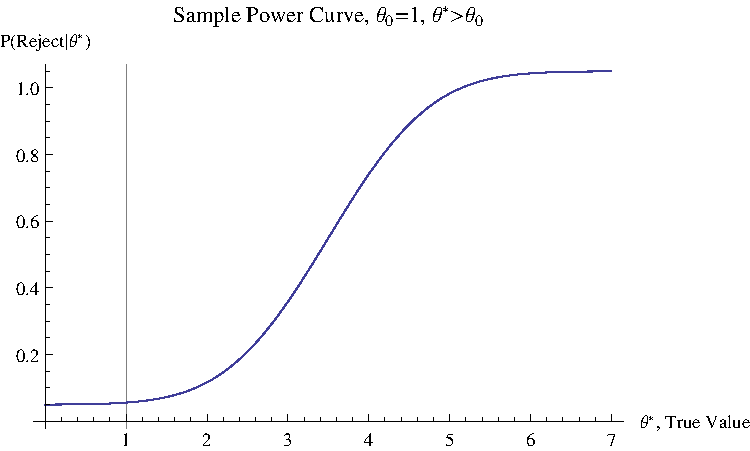
\includegraphics[scale=0.7]{SamplePowerCurve.pdf}
%\end{figure}

\subsection{Neyman-Pearson Lemma}

{\sl Simple $H_0$, Simple $H_1$}: We first consider the case where
both the null and alternative are simple, and we denote the jdfs
implied by $H_0$ and $H_1$ as $f_0$ and $f_1$, respectively. We
then form the \emph{likelihood ratio}:
\[ \text{LR} = \frac{f_0(y_1, \ldots, y_n)}{f_1(y_1, \ldots, y_n)}=
   \frac{P(\text{data under $H_0$})}{P(\text{data under $H_1$})}
   \]
The Neyman-Pearson Lemma states that the uniformly most powerful
test of $H_0$ versus $H_1$ rejects $H_0$ whenever LR $\leq K$,
where $K$ is ``sufficiently small'' given the chosen value of $\alpha$.
And by ``uniformly most powerful,'' we mean that this test
maximizes the power (i.e. is \emph{optimal})
after controlling for the Type I error---i.e.
after setting the Type I error rate to $\alpha$.
\\
\\
{\sl Connection to Sufficient Statistics}: If a sufficient statistic,
$W$, exists for the parameter, $\theta$, that's being tested, then
$W$ \emph{will} be the test statistic in the hypothesis test. This
follows from the fact that we can factorize the jdf into two
components: a function of the data only and a function of the sufficient
statistic and $\theta$.

\subsection{Lambda Ratio Test}

\subsubsection{Justification and Intuition}

Recall that the Neyman-Pearson lemma stated that the method gave
the uniformly most powerful tests. However, recall that power\footnote{
Unlimited power!} is defined as
   \[ \text{Power} = P(\text{Reject $H_0$} | \text{$H_1$ true}) \]
Moreover the likelihood Ratio procedure required a specification
of the probability of the data under the alternative, $H_1$. BUT,
and here's the rub, is you're working with a \emph{composite}
alternative, where not all parameters are specified
\begin{enumerate}
   \item Power is not a single number, but a range of values
      depending upon the values in $H_1$, which can vary.
   \item The probability of the data under the alternative \emph{also}
      takes on a range of values.
\end{enumerate}
How to cope?
\\
\\
Well, if you wanted to know who had the best Hockey players---the US
or Canada---it's not very efficient to have all teams consisting of
all hockey players compete against each other. So you take the
all-stars, and have the best of the US play against the best Canadian
players.  We'll essentially do the same here.

\subsubsection{Procedure}

So suppose the null and alternative hypothesis are composite.
We now form the Lambda Ratio by taking
\[ \lambda =
   \frac{\max P(\text{data under $H_0$})}{
      \max P(\text{data under $H_1$})}
   \]
To find the maximum probabilities under $H_0$ and $H_1$, we
will have to differentiate the likelihood---or equivalently, the
log-likelihoods---with respect to any unspecified parameters, set
the first order conditions equal to zero, and solve.
\\
\\
After we have the solutions, we plug back into the $\lambda$ formula
and use the same criterion:
reject $H_0$ whenever $\lambda\leq K$,
where $K$ is ``sufficiently small'' given the chosen value of $\alpha$.
This maximizes the power after controlling for the Type I error---i.e.
after setting the value of the Type I error equal to $\alpha$.


\clearpage
\section{Classical Linear Regression: Finite Samples Properties of OLS}

\subsection{Setup and Assumptions}

In this section, I follow Hayashi and assume that the $n\times k$
regressor matrix $\bsX$ is \emph{random} rather than fixed, since that
seems more appropriate for a non-experimental discipline like economics
where the RHS ``independent'' variables are not under the control of the
econometrician.


\begin{defn}(Classical Linear Regression Model)
For a sample of $N$ observations and $K$ regressors, the
\emph{classical linear regression model} satisfies the following
assumptions. Note that the sample $\{(y_n,\bsx_n)\}\nN$ is not
necessarily assumed iid. The joint distribution of $(y_n,\bsx_n)$ could
depend on $n$, as it likely would for time series data, though the
assumptions we now state are not necessarily \emph{good} assumptions for
such applications.
\begin{enumerate}
  \item Linearity: We assume the model can be written
    \begin{align}
      \underbrace{\bsy}_{(N\times 1)}
      =
      \underbrace{\vphantom{\bsy} \bsX}_{(N\times K)}
      \underbrace{\vphantom{\bsy} \bsbeta}_{(K\times 1)}
      + \underbrace{\vphantom{\bsy} \bsvarepsilon}_{(N\times 1)}
      \label{regyx}
    \end{align}
  \item Strict Exogeneity: $\E[\varepsilon_n |\bsX]=0$ for
    $n=1,\ldots,N$.

    Note that error $\varepsilon_n$ for observation $n$ is
    mean zero conditional on \emph{all} observations in $\bsX$, not just
    $\bsx_n$.
    And it doesn't matter here that we're restricting them to the
    constant zero rather than some other constant, so long as we have an
    intercept in the model.

    Consequences of this assumption are that the errors are
    unconditinally mean zero and \emph{each} error term is orthogonal to
    the regressors of \emph{any} observation, hence uncorrelated:
    \begin{align*}
      \E[\varepsilon_n] &= \E[\E[\varepsilon_n|\bsX]] = 0 \\
      \E[\bsx_m \cdot \varepsilon_n] &=
      \E[\E[\bsx_m \cdot \varepsilon_n|\bsX]] =
      %\E[\bsx_m\E[ \varepsilon_n|\bsX]] = \underbrace{\bso}_{K\times 1}
      \E[\bsx_m\E[ \varepsilon_n|\bsX]] = \bso
      \qquad \forall n,m = 1,\ldots,N \\
      \Cov(\varepsilon_n, x_{mk})
      &=
      \E[\varepsilon_n x_{mk}] - \E[\varepsilon_n]\E[x_{mk}] = 0
    \end{align*}
    In general, strict exogeneity is a bad assumption for time series
    models.

  \item No multicolinearity: $P[\rank(\bsX)=K]=1$, full column
    rank.\footnote{%
      This implies that $\bsX'\bsX$ is positive definite. First, define.
      $\bsb:=\bsX \bsa$. By the full rank assumption, there is no linear
      combination of columns such that $\bsb=\bsX\bsa = \bso$.
      Therefore, for all $\bsa\neq \bso$, we have
      $\bsa'\bsX'\bsX\bsa=\bsb'\bsb = \sum_{k=1}^K b_k^2 > 0$, so we can
      say that $\bsX'\bsX$ is positive definite.
    }

  \item Spherical Error Variance (Optional): Errors are both
    homoskedastic and uncorrelated:
    \begin{align*}
      \Var(\bsvarepsilon|\bsX) =
      \E[\bsvarepsilon\bsvarepsilon'|\bsX] = \sigma^2\bsI_N
    \end{align*}
    where $\bsI_N$ is the $N$-dimensional identity matrix.

    Coupled with strict exogeneity, homoeskedasticy implies constant
    conditional error variance $\Var(\varepsilon_n|\bsX)=\sigma^2$,
    while uncorrelated errors implies no serial correlation
    in the error terms $\Cov(\varepsilon_n,\varepsilon_m)=0$.
\end{enumerate}
\end{defn}

\clearpage
\begin{defn}(Conditional and Unconditional Homoskedasticity)
Given the classical regression model, we define two concepts for
homoskedasticity that differ subtly in the Hayashi random-$\bsX$
approach:
\begin{enumerate}
  \item \emph{Unconditional homoskedasticity}:
    $\E[\varepsilon_n^2] = \sigma^2$ for all $n$.
  \item \emph{Conditional Homoskedasticity}:
    $\E[\varepsilon_n^2 | \bsx_n]
    =\E[\varepsilon_n^2 | \bsX] = \sigma^2$
\end{enumerate}
Most importantly, we can have unconditional homoskedasticity
(i.e.\ $\E[\varepsilon_n^2]=\sigma^2$ a constant) \emph{without}
conditional homoskedasticity (i.e.\ $\E[\varepsilon_n^2|\bsx_n]$
\emph{not} a constant).  In particular, the \emph{conditional} second
moment $\E[\varepsilon_n^2|\bsx_n]$ could be a \emph{function}---not
just a number/constant---that depends on $\bsx_n$. For example, maybe it
blows up for small and large values of $\bsx_n$ but it does so
symmetrically, so that the average
$\E[\varepsilon_n^2]=\E[\E[\varepsilon_n^2|\bsx_n]]=\sigma^2$.

We need to make this distinction because Hayashi assumes $\bsX$
is random. His formulation is not a ``fixed $\bsX$'' approach, where
Assumptions 2 and 4 are merely $\E[\varepsilon_i]=0$ and
$\E[\bsvarepsilon\bsvarepsilon']=\sigma^2\bsI_N$ without the
conditioning.
\end{defn}

\begin{defn}(Classical Regression Model with Random Samples)
The classical regression model with random sampling assumes that the
sample $\{(y_n,\bsx_n)\}\nN$ is iid across observations.

First, Assumption 1 along with the iid assumption on
$(y_n,\bsx_n)$ implies that $(\varepsilon_n, \bsx_n)\perp \bsx_m$ for
$n\neq m$.
So Assumptions 1 and 4 on $\varepsilon_n$ (which we always
conditioned on $\bsX$) will simplify to conditioning on individual
$\bsx_n$:
\begin{alignat*}{5}
  \text{Assumption 2} &&\qquad
   \E[\varepsilon_n | \bsX] &=
   \E[\varepsilon_n | \bsx_n] &&= 0\\
  \text{Assumption 4} &&\qquad
   \E[\varepsilon_n^2 | \bsX] &=
   \E[\varepsilon_n^2 | \bsx_n] &&= \sigma^2\\
  \text{} &&\qquad
   \E[\varepsilon_n\varepsilon_m|\bsX] &=
   \E[\varepsilon_n|\bsx_n] \E[\varepsilon_m|\bsx_m]
   &&=0
\end{alignat*}
Moreover, these objects (which are, in general, functions of $\bsx_n$)
will be identical across observations.

Now it might seem like $\E[\varepsilon_n^2|\bsx_n]=\sigma^2$ (i.e.\
conditional homosekedasticy) is an unnecessary and worthless assumption,
since it would seem to follow \emph{immediately} from assuming iid
observations. In the ``fixed-$\bsX$'' approach, this is certainly true,
but in Hayashi's ``random-$\bsX$'' approach, this is not true for the
reasons mentioned above.

Assuming an iid sample only ensures that $\E[\varepsilon_n^2|\bsx_n]$ is
identical across observations.  But, in general, that guy is a function
of random variable $\bsx_n$.  Though identical across observations, that
function is not necessarily a number/constant. Of course, if we iterate
expectations and integrate out $\bsx_n$ by computing
$\E[\varepsilon_n^2]=\E[\E[\varepsilon_n^2|\bsx_n]]$, the result will be
a constant. Hence, an iid sample implies \emph{unconditional}
homoskedasticity. But as we said above, the iid sample assumption does
not automatically imply \emph{conditional} homoskedasticity where
$\E[\varepsilon_n^2 | \bsx_n]
=\E[\varepsilon_n^2 | \bsX] = \sigma^2$.
Therefore, assuming $\E[\varepsilon_n^2|\bsx_n]=\sigma^2$ a constant
still has some bite.
\end{defn}

\clearpage
\subsection{Estimation}

\begin{defn}(Sum of Squared Residuals)
Define the \emph{sum of squared residuals} as
\begin{align*}
  SSR(\bsb) = (\bsy - \bsX \bsb)'(\bsy - \bsX \bsb)
\end{align*}
\end{defn}


\begin{defn}(OLS Estimates)
The \emph{OLS Estimator} minimizes the sum of squared residuals:
\begin{align*}
  \bshatbeta_{OLS}
  =
  \argmin_{\bsb} \;
  (\bsy - \bsX \bsb)'(\bsy - \bsX \bsb)
\end{align*}
The FOCs of $K$ equations and $K$ unknowns are called the
\emph{normal equations}, where the second expression highlights the
orthogonality of the regressors $\bsX'$ to the residual vector
$\bsy-\bsX\bsb$.  Since the second derivative is the positive definite
matrix $\bsX'\bsX$, we have a minimum.
\begin{align*}
  \bsX'\bsX\bsb &= \bsX'\bsy
  \quad\iff\quad
  0= \bsX'(\bsy-\bsX\bsb)
\end{align*}
Solving, we get the OLS estimator, which has the following mean and
variance:
\begin{align*}
  \hat{\bsbeta}_{OLS}
  &= (\bsX'\bsX)^{-1}\bsX'\bsy \\
  &= (\bsX'\bsX)^{-1}\bsX' (\bsX \bsbeta + \bsvarepsilon)
  = \bsbeta + (\bsX'\bsX)^{-1}\bsX' \bsvarepsilon
  \\
  \implies\quad
  \hat{\bsbeta}_{OLS} - \bsbeta
  &= (\bsX'\bsX)^{-1}\bsX' \bsvarepsilon \\
  \E[\hat{\bsbeta}_{OLS}|\bsX]
  %&=
  %\bsbeta +
  %\E[(\bsX'\bsX)^{-1}\bsX' \bsvarepsilon |\bsX]
  %=
  %\bsbeta +
  %(\bsX'\bsX)^{-1}\bsX' \cdot \E[\bsvarepsilon |\bsX]
  %\\
  &= \bsbeta \\
  \Var(\hat{\bsbeta}_{OLS}|\bsX)
  &=
  \E[(\hat{\bsbeta}_{OLS}-\bsbeta)(\hat{\bsbeta}_{OLS}-\bsbeta)'|\bsX]
  \\
  %&=
  %\E\left[
    %(\bsX'\bsX)^{-1}\bsX'\bsvarepsilon)
    %(\bsX'\bsX)^{-1}\bsX'\bsvarepsilon)'
  %|\bsX\right]
  %\\
  &=
  \left((\bsX'\bsX)^{-1}\bsX'\right)
  \E[\bsvarepsilon\bsvarepsilon' |\bsX]
  \left(\bsX(\bsX'\bsX)^{-1}\right)
\end{align*}
With spherical errors, the variance simplifies to
\begin{align*}
  \Var(\hat{\bsbeta}_{OLS}|\bsX)
  &=
  \left((\bsX'\bsX)^{-1}\bsX'\right)
  \sigma^2 \bsI_N
  \left(\bsX(\bsX'\bsX)^{-1}\right)
  =\sigma^2 (\bsX'\bsX)^{-1}
\end{align*}
Now define the following objects
\begin{alignat*}{3}
  \text{Projection Matrix}&\quad
  \bsP &&= \bsX(\bsX'\bsX)^{-1}\bsX' \\
  \text{Annihilator Matrix}&\quad
  \bsM &&= \bsI_n - \bsP \\
  \text{Residual Vector}&\quad
  \bse &&= \bsX\bsb - \bsy \\
  \text{Fitted Values}&\quad
  \bshaty &&= \bsX\bsb
\end{alignat*}
Both $\bsP$ and $\bsM$ are easily shown to be symmetric and idempotent.
Moreover,
\begin{itemize}
  \item $SSR(\bsb) = \bse'\bse$
  \item $\bsP\bsX=\bsX$: The projection of $\bsX$ onto itself is $\bsX$
  \item $\bsM\bsX = \bso$: This is where the annihilator matrix gets
    it's name.
  \item $\bse = \bsM\bsy = \bsM \bsvarepsilon$: Applied to $\bsy$, the
    annihilator matrix returns the residuals
\end{itemize}
\end{defn}

\begin{defn}(Distribution of Coefficients)
If we want the mean and variance of individual coefficients or linear
combinations of coefficients, we have
\begin{align*}
  \E[r'\bshatbeta_{OLS}|\bsX]
  &= r'\bsbeta \\
  \Var(r'\bshatbeta_{OLS}|\bsX)
  &=
  r'\left((\bsX'\bsX)^{-1}\bsX'\right)
  \E[\bsvarepsilon\bsvarepsilon' |\bsX]
  \left(\bsX(\bsX'\bsX)^{-1}\right) r \\
  &=
  \sigma^2r'(\bsX'\bsX)^{-1} r
\end{align*}
where the second formula for the variance assumed spherical errors. The
first expression is more general.
\end{defn}

\begin{defn}(Estimator for $\sigma^2$ and $\Var[\hat{\bsbeta}_{OLS}|\bsX]$)
Assuming spherical errors, we form the estimator for $\sigma^2$:
\begin{align*}
  s^2 &= \frac{SSR(\bsb)}{(n-K)} = \frac{\bse'\bse}{(N-K)}
\end{align*}
That let's us define an estimator for the covariance matrix of the
coefficients:
\begin{align*}
  \bshatV(\hat{\bsbeta}_{OLS}|\bsX) = s^2(\bsX'\bsX)^{-1}
\end{align*}
\end{defn}

\begin{prop}
Assuming spherical errors, $s^2$ is an unbiased estimator:
$\E[s^2|\bsX]=\sigma^2$.
\end{prop}
\begin{proof}
Recall that $\bse=\bsM\bsvarepsilon$ where $\bsM$, the annihilator
matrix, is idempotent. Then
\begin{align*}
  \E[\bse'\bse|\bsX]
  &= \E[\bsvarepsilon'\bsM'\bsM\bsvarepsilon|\bsX]\\
  &= \E[\bsvarepsilon'\bsM\bsvarepsilon|\bsX] \\
  &= \sumin \sumjn m_{ij}\E[\varepsilon_i\varepsilon_j|\bsX]
\end{align*}
But since we assumed $\E[\varepsilon_i\varepsilon_j|\bsX]=0$, all cross
terms drop, leaving
\begin{align*}
  \E[\bse'\bse|\bsX]
  &= \sumin m_{ii}\E[\varepsilon_i\varepsilon_i|\bsX]
  = \sumin m_{ii}\sigma^2 \\
  &= \sigma^2 \cdot \trace(\bsM)
\end{align*}
Almost there. Just use the definition of $\bsM$:
\begin{align*}
  \E[\bse'\bse|\bsX]
  &= \sigma^2 \cdot \trace(\bsM) \\
  &= \sigma^2 \trace(\bsI_N - \bsX(\bsX'\bsX)^{-1}\bsX') \\
  &= \sigma^2 \trace(\bsI_N) - \trace(\bsX(\bsX'\bsX)^{-1}\bsX') \\
  \text{By $\trace(AB)=\trace(BA)$}\qquad
  &= \sigma^2 \left(N - \trace(\bsX'\bsX(\bsX'\bsX)^{-1})\right) \\
  \E[\bse'\bse|\bsX]
  &= \sigma^2 \left(N - \trace(\bsI_K)\right)
  = \sigma^2 \left(N - K\right)
\end{align*}
Therefore,
\begin{align*}
  \E[\bse'\bse|\bsX] = \sigma^2(N-K)
  \quad\implies\quad
  \E[s^2|\bsX] = \frac{\E[\bse'\bse|\bsX]}{N-K} = \sigma^2
\end{align*}




\end{proof}



\clearpage
\subsection{Gauss-Markov Theorem}

\begin{thm}\emph{(Gauss-Markov)}
Given the classical linear regression model assuming spherical errors
$\Var(\bsvarepsilon|\bsX)=\sigma^2\bsI$, the OLS estimator is
\emph{efficient} in the class of linear unbiased estimators. That is,
\begin{align*}
  \bstildebeta = \bsA\bsy
  \quad \text{s.t}\quad \E[\bstildebeta]=\bsbeta
  \quad\implies\quad
  \Var(\bstildebeta|\bsX) \geq \Var(\bshatbeta|\bsX)
\end{align*}
where $\bsA$ is some constant (nonrandom) matrix that can depend upon
$\bsX$, and $\bshatbeta$ is the OLS estimator.
\end{thm}
\begin{proof}
($\bstildebeta$ Unbiased $\implies$ $\bsA\bsX=\bsI$)
First, we want to show a mini-result. Start by writing out the
expectation of $\bstildebeta$:
\begin{align*}
  \E[\bstildebeta|\bsX]
  &= \E[\bsA\bsy|\bsX]
  = \E[\bsA(\bsX\bsbeta +\varepsilon)|\bsX] \\
  \implies\quad
  \E[\bstildebeta|\bsX]
  &= \bsA\bsX\bsbeta
\end{align*}
Therefore, if $\bstildebeta$ is to be an unbiased estimator of
$\bsbeta$, we need must have $\bsA\bsX=\bsI$.
\\
\\
($\Cov(\bshatbeta, \bstildebeta-\bshatbeta|\bsX)=0$)
Next, we show another mini-result. To do so, we consider
$\bstildebeta-\bshatbeta$ and use the result that $\bsA\bsX=\bsI$ along
with regression equation $\bsy=\bsX\bsbeta+\bsvarepsilon$ to simplify
the difference:
\begin{align}
  \bstildebeta - \bshatbeta
  &= \bsA\bsy - ((\bsX'\bsX)^{-1}\bsX'\bsy) \notag\\
  %&= (\bsA-(\bsX'\bsX)^{-1}\bsX)\bsy \\
  &= (\bsA-(\bsX'\bsX)^{-1}\bsX')(\bsX\bsbeta + \bsvarepsilon) \notag\\
  &= \bsA\bsX\bsbeta-(\bsX'\bsX)^{-1}\bsX'\bsX\bsbeta
    + (\bsA-(\bsX'\bsX)^{-1}\bsX')\bsvarepsilon \notag \\
  %&= \bsI\bsbeta-\bsI\bsbeta
    %+ (\bsA-(\bsX'\bsX)^{-1}\bsX)\bsvarepsilon \\
  \implies\quad
  \bstildebeta - \bshatbeta
  &= (\bsA-(\bsX'\bsX)^{-1}\bsX')\bsvarepsilon
  \label{betatilde-betahat}
\end{align}
Moreover, since both $\bshatbeta$ and $\bstildebeta$ are unbiased
estimators, we have
\begin{align*}
  \E[\bshatbeta|\bsX] = \E[\bstildebeta|\bsX] &= \bsbeta \\
  \E[\bshatbeta-\bstildebeta|\bsX] &= 0
\end{align*}
We now compute the covariance between $\bshatbeta$ and
$\bstildebeta-\bshatbeta$. We will use the simplified formula from above
for $\bstildebeta-\bshatbeta$, the means just stated, and the formula
derived in the estimation section above that
$\bshatbeta-\bsbeta=(\bsX'\bsX)^{-1}\bsX'\bsvarepsilon$ in the covariance
formula:
\begin{align*}
  \Cov(\bstildebeta - \bshatbeta,\bshatbeta|\bsX)
  &=
  \E\left[
    (\bstildebeta - \bshatbeta)
    (\bshatbeta-\bsbeta)'
    |\bsX\right]
  \\
  &=
  \E\left[
    \left((\bsA-(\bsX'\bsX)^{-1}\bsX')\bsvarepsilon\right)
    \left((\bsX'\bsX)^{-1}\bsX'\bsvarepsilon\right)'
    |\bsX\right]
  \\
  &=
  (\bsA-(\bsX'\bsX)^{-1}\bsX')
    \E\left[ \bsvarepsilon \bsvarepsilon'|\bsX\right]
    \left(\bsX(\bsX'\bsX)^{-1}\right)
\end{align*}
Under spherical errors
$\E\left[\bsvarepsilon\bsvarepsilon'|\bsX\right]=\sigma^2\bsI$,
therefore
\begin{align*}
  \Cov(\bstildebeta - \bshatbeta,\bshatbeta|\bsX)
  &=
  \sigma^2
  (\bsA-(\bsX'\bsX)^{-1}\bsX')
    \left(\bsX(\bsX'\bsX)^{-1}\right)
  \\
  &=
  \sigma^2
  \bsA \bsX(\bsX'\bsX)^{-1}
  -(\bsX'\bsX)^{-1}
  \\
  \text{Since $\bsA\bsX=\bsI$}\qquad
  &=
  \sigma^2
  \bsI(\bsX'\bsX)^{-1}
  -(\bsX'\bsX)^{-1} \\
  \implies\quad
  \Cov(\bstildebeta - \bshatbeta,\bshatbeta|\bsX)
  &= 0
\end{align*}
(Final Step)
Okay, now compute the variance of $\bstildebeta$:
using the fact that covariance equals zero
\begin{align*}
  \Var(\bstildebeta|\bsX)
  &=
  \Var(\bshatbeta + (\bstildebeta-\bshatbeta)|\bsX) \\
  &=
  \Var(\bshatbeta|\bsX) + \Var(\bstildebeta-\bshatbeta)|\bsX)
  + 2\Cov(\bstildebeta-\bshatbeta,\,\bshatbeta|\bsX)\\
  \implies\quad
  \Var(\bstildebeta|\bsX)
  &=
  \Var(\bshatbeta|\bsX) + \Var(\bstildebeta-\bshatbeta)|\bsX)
\end{align*}
Therefore, the variance of $\bstildebeta$, an arbitrary linear unbiased
estimator, is greater than the variance of $\bshatbeta$ by the positive
semidefinite matrix $\Var(\bstildebeta-\bshatbeta|\bsX)$.
\\
\\
If we want to answer ``How much bigger?'', we can simplify the
expression for the variance using Expression~\ref{betatilde-betahat}:
\begin{align*}
  \Var(\bstildebeta-\bshatbeta)|\bsX)
  &=
  \Var((\bsA-(\bsX'\bsX)^{-1}\bsX')\bsvarepsilon|\bsX) \\
  &=
  (\bsA-(\bsX'\bsX)^{-1}\bsX')
  \;\Var(\bsvarepsilon|\bsX)\;
  (\bsA-(\bsX'\bsX)^{-1}\bsX')' \\
  &=
  \sigma^2 (\bsA-(\bsX'\bsX)^{-1}\bsX')
  (\bsA-(\bsX'\bsX)^{-1}\bsX')'
\end{align*}
Where the last line used the assumption of spherical errors
$\Var(\bsvarepsilon|\bsX)=\sigma^2\bsI$.
\end{proof}


\clearpage
\subsection{$R^2$ and Relatives}

\begin{defn}($R^2$)
First, We define the \emph{uncentered $R^2$} via the decomposition
\begin{align*}
  \bsy' \bsy
  &=
  (\bshaty +\bse)'
  (\bshaty +\bse) \\
  &=
  \bshaty' \bshaty
  +2 \bshaty'\bse
  +\bse'\bse \\
  \text{From orthogonality condtion} \quad
  &=
  \bshaty' \bshaty
  +\bse'\bse \\
  \implies\quad
  R^2_{uc}
  &=
  \frac{\bshaty' \bshaty}{\bsy' \bsy}
  = 1- \frac{\bse'\bse}{\bsy' \bsy}
\end{align*}
This is guaranteed to lie in $[0,1]$.
\\
\\
Next, we define the \emph{centered $R^2$} or
\emph{coefficient of determination}.
\begin{align*}
  (\bsy-\bar{\bsy})'(\bsy-\bar{\bsy})
  &=
  (\bshaty-\bar{\bsy})'(\bsy-\bar{\bsy})
  +
  \bse'\bse \\
  \implies\quad
  R^2
  &=
  1-
  \frac{\bse'\bse}{(\bsy-\bar{\bsy})'(\bsy-\bar{\bsy})}
  =
  \frac{(\bshaty-\bar{\bsy})'(\bsy-\bar{\bsy})}{%
      (\bsy-\bar{\bsy})'(\bsy-\bar{\bsy})}
\end{align*}
Note that this guy can go negative if you don't include an intercept
term in the regression.
\\
\\
We now define \emph{adjusted $R^2$}, which penalizes the number of
regressors:
\begin{align*}
  R^2_A = 1 -
  \frac{\bse'\bse/(N-K)}{(\bsy-\bar{\bsy})'(\bsy-\bar{\bsy})/(N-1)}
\end{align*}
\end{defn}

\clearpage
\subsection{Heteroskedasticity Robust Standard Errors}

Without assuming spherical errors (homoskedasticity), recall that
the variance of the OLS estimator is
\begin{align*}
  \Var(\hat{\bsbeta}_{OLS}|\bsX)
  &=
  \left((\bsX'\bsX)^{-1}\bsX'\right)
  \E[\bsvarepsilon\bsvarepsilon' |\bsX]
  \left(\bsX(\bsX'\bsX)^{-1}\right) \\
  %&=
  %(\bsX'\bsX)^{-1}
  %\E[\bsX'\bsvarepsilon\bsvarepsilon'\bsX\;|\;\bsX]
  %(\bsX'\bsX)^{-1}
  %\\
  &=
  (\bsX'\bsX)^{-1}
  \E\left[
  \left(
  \sumnN \varepsilon_n \bsx_n
  \right)
  \left(
  \sumnN \varepsilon_n \bsx_n
  \right)'
  \;\bigg|\;\bsX
  \right]
  (\bsX'\bsX)^{-1} \\
  &=
  (\bsX'\bsX)^{-1}
  \E\left[
  \sumnN
  \sum_{m=1}^N
  \varepsilon_n\varepsilon_m \bsx_n\bsx_m'
  \big|\bsX
  \right]
  (\bsX'\bsX)^{-1} \\
  \implies\quad
  \Var(\hat{\bsbeta}_{OLS}|\bsX)
  &=
  (\bsX'\bsX)^{-1}
  \E\left[
  \sumnN
  \varepsilon_n^2 \bsx_n\bsx_n'
  \;\big|\;\bsX
  \right]
  (\bsX'\bsX)^{-1}
\end{align*}
where got to the last line by using the fact that
$\E[\varepsilon_n\varepsilon_m|\bsX]=0$ for $n\neq m$.
\\
\\
To esitmate this object, we form the natural estimator called the
\emph{sandwich estimator}:
\begin{align*}
  \bshatV(\hat{\bsbeta}_{OLS}|\bsX)
  =
  (\bsX'\bsX)^{-1}
  \left(
  \sumnN
  e_n^2 \bsx_n\bsx_n'
  \right)
  (\bsX'\bsX)^{-1}
\end{align*}
using the estimated errors $e_n$.


\clearpage
\subsection{Omitted Variable Bias}

Suppose that the true model is
\begin{align*}
  \bsy = \bsX\bsbeta + \bsZ \bsgamma + \bsvarepsilon
\end{align*}
but we run the regression
\begin{align*}
  \bsy = \bsX\bsbeta + \bsvarepsilon
\end{align*}
Then the OLS estimates are
\begin{align*}
  \bshatbeta
  &= (\bsX'\bsX)^{-1}\bsX' \bsy \\
  &= (\bsX'\bsX)^{-1}\bsX'
    \left(\bsX\bsbeta + \bsZ \bsgamma + \bsvarepsilon\right) \\
  \bshatbeta - \bsbeta
  &= (\bsX'\bsX)^{-1}\bsX'
    \left(\bsZ \bsgamma + \bsvarepsilon\right)
\end{align*}
This implies bias
\begin{align*}
  \E\left[\bshatbeta - \bsbeta\;|\;\bsX,\bsZ\right]
  &= (\bsX'\bsX)^{-1} \bsX'\bsZ \bsgamma
\end{align*}
The bias is zero if and only if $\bsgamma=0$ (variables in $\bsZ$ do not
affect $\bsy$) or $\bsX'\bsZ=0$ (the ommited variables are orthogonal to
those included).



\clearpage
\subsection{Coefficient Restrictions}

Suppose that we have linear regression model
\begin{align*}
  \bsy = \bsX\bsbeta + \bsvarepsilon
\end{align*}
and we want to estimate $\bsbeta$ while also imposing some restrictions
$\bsR'\bsbeta = \bsr$, where $\bsR\in\R^{K\times C}$ is a matrix of $C$
constraints on the $K$ coefficients. We assume that $\rank(\bsR)=C$
(full column rank), otherwise there would be redundant constraints that
could be removed without effect.
\\
\\
We estimate by constrained least squares
\begin{align*}
  \min_{\bsb} \; &(\bsy-\bsX\bsb)'(\bsy-\bsX\bsb)
  \\
  \text{s.t.} \; &
    \bsR'\bsb = \bsr
\end{align*}
whose solution we call $\bshatbeta_*$, while $\bshatbeta_{OLS}$
represents the unrestricted OLS estimator.
The basic estimates are
\begin{align*}
  \bshatbeta_*
  &=
  \bshatbeta_{OLS} - \left(\bsX'\bsX\right)^{-1}  \bsR
  \left(\bsR'\left(\bsX'\bsX\right)^{-1}  \bsR\right)^{-1}
  \left(\bsR'\bshatbeta_{OLS} -  \bsr\right)
  \\
  \Var[\bshatbeta_*\;|\;\bsX]
  &=
  \underbrace{\sigma^2(\bsX'\bsX)^{-1}}_{\Var(\bshatbeta_{OLS}|\bsX)}
  -
  \sigma^2(\bsX'\bsX)^{-1}  \bsR
  \left(\bsR'(\bsX'\bsX)^{-1}  \bsR\right)^{-1} \bsR'(\bsX'\bsX)^{-1}
  \\
  \Var\left[ \bshatbeta_*-\bshatbeta_{OLS} \;|\;X\right]
  &=
  \sigma^2
  \left(\bsX'\bsX\right)^{-1}  \bsR
  \left(\bsR'\left(\bsX'\bsX\right)^{-1}  \bsR\right)^{-1} \bsR'
  \left(\bsX'\bsX\right)^{-1}
\end{align*}
Since the term subtracted from $\Var[\bshatbeta_{OLS}\;|\;\bsX]$ in the
expression for $\Var[\bshatbeta_*\;|\;\bsX]$ is a positive semidefinite
matrix, the constrained estimates have a smaller variance than the OLS
estimates (though they are biased).


\begin{proof}
Form the Lagrangian
\begin{align*}
  \sL
  &=
  (\bsy-\bsX\bsb)'(\bsy-\bsX\bsb)
  + 2\bslambda' (\bsR'\bsb - \bsr)
\end{align*}
where $\bslambda$ is a vector the same size as $\bsr$ (possibly also length
one, i.e.\ a scalar).
The first order conditions of the Lagrangian with respect to $\bsb$:
\begin{align*}
  \frac{d}{d\bsb}
  \left[
    (\bsy-\bsX\bsb)'(\bsy-\bsX\bsb)
    + 2\bslambda' (\bsR'\bsb - \bsr)
  \right]
  &= -2\bsX'\bsy +2\bsX'\bsX\bsb + 2\bsR\bslambda
  =0
\end{align*}
Solve for $\bsb$
\begin{align}
  \bsb &=
  \left(\bsX'\bsX\right)^{-1} \bsX'\bsy
  - \left(\bsX'\bsX\right)^{-1} \bsR\bslambda
  \notag\\
  \implies\quad
  \bsb &=
  \bshatbeta_{OLS} - \left(\bsX'\bsX\right)^{-1}  \bsR\bslambda
  \label{restricted-b}
\end{align}
To eliminate $\bslambda$, we will multiply through the above expression
by $\bsR'$ and use the constraint $\bsR'\bsb=\bsr$ on the LHS to get
\begin{align}
  %\bsR'\bsb
  %&=
  %\bsR'\bshatbeta_{OLS}
  %- \bsR'\left(\bsX'\bsX\right)^{-1} \bsR\bslambda \notag\\
  %\iff\quad
  \bsr
  &=
  \bsR'\bshatbeta_{OLS}
  - \bsR'\left(\bsX'\bsX\right)^{-1} \bsR\bslambda \notag\\
  \implies\quad
  \bslambda
  &=
  \left(\bsR'\left(\bsX'\bsX\right)^{-1}  \bsR\right)^{-1}
  \left(\bsR'\bshatbeta_{OLS} -  \bsr\right)
  \label{restricted-lambda}
\end{align}
where $\bsR'(\bsX'\bsX)^{-1}\bsR$ is invertible because
$(\bsX'\bsX)^{-1}$ is positive definite and $\bsR$ has full column rank.
Now sub Expression~\ref{restricted-lambda} for $\bslambda$ into
Expression~\ref{restricted-b} for $\bsb$:
\begin{align*}
  \bshatbeta_*
  =
  \bshatbeta_{OLS} - \left(\bsX'\bsX\right)^{-1}  \bsR
  \left(\bsR'\left(\bsX'\bsX\right)^{-1}  \bsR\right)^{-1}
  \left(\bsR'\bshatbeta_{OLS} -  \bsr\right)
\end{align*}
This estimator has expectation
\begin{align*}
  \E\left[ \bshatbeta_* \;|\; \bsX \right]
  &=
  \bsbeta
  -
  \left(\bsX'\bsX\right)^{-1}  \bsR
  \left(\bsR'\left(\bsX'\bsX\right)^{-1}  \bsR\right)^{-1}
  \left( \bsR' \bsbeta -  \bsr\right)
\end{align*}
Next, we compute the variance of the estimator:
\begin{align*}
  \Var[\bshatbeta_*\;|\;\bsX]
  &=
  \E\left[
    \left(\bshatbeta_*- \E[\bshatbeta_*|\bsX]\right)^2
  \;|\;\bsX \right] \\
  &=
  \E\bigg[
  \bigg\{
  \left[
  \bshatbeta_{OLS} - (\bsX'\bsX)^{-1}  \bsR
  \left(\bsR'(\bsX'\bsX)^{-1}  \bsR\right)^{-1}
  \left(\bsR'\bshatbeta_{OLS} -  \bsr\right)
  \right]\\
  &\qquad\quad
  -
  \left[
  \bsbeta -
  (\bsX'\bsX)^{-1}  \bsR \left(\bsR'(\bsX'\bsX)^{-1}\bsR\right)^{-1} \left(\bsR' \bsbeta -\bsr\right)
  \right]
  \bigg\}^2
  \;\big|\;\bsX
  \bigg] \\
  \Var[\bshatbeta_*\;|\;\bsX]
  &=
  \left(
  \bsI - (\bsX'\bsX)^{-1}  \bsR \left(\bsR'(\bsX'\bsX)^{-1}  \bsR\right)^{-1} \bsR'
  \right)
  \E\left[ (\bshatbeta_{OLS}-\bsbeta)^2 \;\big|\;\bsX \right]
  \left(
  \text{Leading term}
  \right)' \\
  &= (\bsI - \bsA)\bsV(\bsI-\bsA)'
  \\
  \text{where}
  \quad
  \bsA &:=
    (\bsX'\bsX)^{-1}  \bsR \big(\bsR'(\bsX'\bsX)^{-1}  \bsR\big)^{-1} \bsR' \\
  \bsV
  &:= \E\left[ (\bshatbeta_{OLS}-\bsbeta)^2 \;\big|\;\bsX \right]
\end{align*}
Note that
$(\bsI-\bsA)\bsV(\bsI-\bsA)'=(\bsV-\bsA\bsV)-(\bsV\bsA'-\bsA\bsV\bsA')$.
We can calculate each of these objects, assuming spherical errors,
otherwise the result doesn't work out nicely
\begin{align*}
  \bsV
  &=
  \E\left[ (\bshatbeta_{OLS}-\bsbeta)^2 \;\big|\;\bsX \right]
  =
  \sigma^2(\bsX'\bsX)^{-1} \\
  \bsA\bsV = (\bsV\bsA')'
  &=
  \sigma^2(\bsX'\bsX)^{-1}  \bsR \left(\bsR'(\bsX'\bsX)^{-1}  \bsR\right)^{-1} \bsR'
  (\bsX'\bsX)^{-1} \\
  \bsA\bsV\bsA'
  &=
  \sigma^2(\bsX'\bsX)^{-1}  \bsR \left(\bsR'(\bsX'\bsX)^{-1}  \bsR\right)^{-1} \bsR'
  (\bsX'\bsX)^{-1}
  \bsR \left(\bsR'(\bsX'\bsX)^{-1}  \bsR\right)^{-1} \bsR'(\bsX'\bsX)^{-1}
  \\
  &=
  \sigma^2(\bsX'\bsX)^{-1}  \bsR
  \left(\bsR'(\bsX'\bsX)^{-1}  \bsR\right)^{-1} \bsR'(\bsX'\bsX)^{-1}
\end{align*}
Hence the variance of the estimator is
\begin{align*}
  \Var[\bshatbeta_*\;|\;\bsX]
  &=
  \underbrace{\sigma^2(\bsX'\bsX)^{-1}}_{\Var(\bshatbeta_{OLS}|\bsX)}
  -
  \sigma^2(\bsX'\bsX)^{-1}  \bsR
  \left(\bsR'(\bsX'\bsX)^{-1}  \bsR\right)^{-1} \bsR'(\bsX'\bsX)^{-1}
\end{align*}
The last one is just a bunch of messy algebra again. It's
straightforward to derive.
\end{proof}


\subsection{Inference under Normal Errors}

\begin{prop}
If we assume
$\bsvarepsilon|\bsX\sim N(0,\sigma^2\bsI)$, then the variance estimator
$s^2$ of $\sigma^2$ has distribution
\begin{align}
  s^2
  = \frac{\bse'\bse}{N-K}
  \sim \frac{\sigma^2}{N-K} \Chi^2_{N-K}
  \label{s2dist}
\end{align}
\end{prop}
\begin{proof}
Since $\bse=\bsM\bsvarepsilon$ where $\bsM$ is the annihilator matrix,
the definition of $s^2$ gives us
\begin{align*}
  (N-K) s^2
  &= \bse' \bse
  = (\bsM\bsvarepsilon)' (\bsM\bsvarepsilon)\\
  &= \sigma^2 \left(\frac{\bsvarepsilon'}{\sigma}\right)\bsM'
    \bsM\left(\frac{\bsvarepsilon}{\sigma}\right)
\end{align*}
Since the matrix $\bsM$ is idempotent, we get
\begin{align*}
  (N-K) \frac{s^2}{\sigma^2}
  &= \left(\frac{\bsvarepsilon'}{\sigma}\right)
    \bsM\left(\frac{\bsvarepsilon}{\sigma}\right)
\end{align*}
Then $\bsvarepsilon/\sigma$, the standardized error vector, is a
multivariate normal distribution.Therefore, the above quadratic form is
$\Chi^2$ with $\rank(\bsM)$ degrees of freedom. But since
$\rank(\bsM)=\trace(\bsM)$ for idempotent matrices like $\bsM$ and
$\trace(\bsM)=N-K$, the desired result follows.
\end{proof}


\begin{defn}(Testing Individual Coefficients)
If we assume $\bsvarepsilon|\bsX \sim N(0,\sigma^2\bsI_N)$, then
\begin{align*}
  \bshatbeta - \bsbeta
  \sim
  N(0,\sigma^2 (\bsX'\bsX)^{-1})
\end{align*}
So we can test whether the $k$th regression coefficient equals
$\beta_{k}^0$ by forming a Z-statistic because, under the null,
\begin{align}
  z_k = \frac{\hat{\beta}_{k} - \beta_{k}^0}{%
      \sqrt{\sigma^2\cdot r_k'(\bsX'\bsX)^{-1}r_k}}
      \sim N(0,1)
  \label{ztest}
\end{align}
where $r_k$ is the $k$th basis element for $\R^K$.

Since $\sigma^2$ is generally unknown, we instead construct a
$t$-statistic using $s^2$, which has a $T_{N-K}$ distribution (see
proof):
\begin{align*}
  t_k = \frac{\hat{\beta}_{k} - \beta_{k}^0}{%
      \sqrt{s^2 \cdot r_k'(\bsX'\bsX)^{-1}r_k}}
    \sim T_{N-K}
\end{align*}
\end{defn}
\begin{proof}
Write out the $t$-statistic:
\begin{align*}
  t_k =
  \frac{\hat{\beta}_{k} - \beta_{k}^0}{%
      \sqrt{s^2 \cdot r_k'(\bsX'\bsX)^{-1}r_k}}
  &=
  \frac{\hat{\beta}_{k} - \beta_{k}^0}{%
      \sqrt{\sigma^2 \cdot r_k'(\bsX'\bsX)^{-1}r_k}}
  \cdot
  \left(
  \sqrt{%
  \frac{s^2}{\sigma^2}
  }
  \right)^{-1} \\
  \text{By Expressions~\ref{s2dist} and \ref{ztest}}\qquad
  &\sim
  N(0,1)
  \cdot
  \left(
  \frac{\Chi^2_{N-K}}{N-K}
  \right)^{-1}
\end{align*}
But the normal and the $\Chi^2$ distribution above are independent
conditional on $\bsX$, so we're done because that's exactly the
definition of a $T_{N-K}$-distribution.
\end{proof}

\begin{defn}($F$-Test)
Suppose we want to test the linear hypothesis
$H_0: \bsR'\bsbeta^0 = \bsr$,
where $\bsR$ is of full column rank and $\bsr$ has dimension $p$,
corresponding to $p$ restrictions.
\\
\\
If we assume spherical errors,
$\bsvarepsilon|\bsX\sim N(0,\sigma^2\bsI_N)$, then under the null, we
know that
\begin{align*}
  \bsR'(\bshatbeta-\bsbeta^0)
  =
  \bsR'\bshatbeta-\bsr
  &\sim N(0,\sigma^2 \bsR'(\bsX'\bsX)^{-1}\bsR)
  %\\
  %\iff\qquad
  %\bsR'\bshatbeta-\bsr
  %&\sim N(0,\sigma^2 \bsR'(\bsX'\bsX)^{-1}\bsR)
\end{align*}
So then we could jointly test whether the following quadratic form is
close to zero
\begin{align*}
  \left(\bsR'\bshatbeta-\bsr\right)'
  \left[\sigma^2 \bsR'(\bsX'\bsX)^{-1}\bsR)\right]^{-1}
  \left(\bsR'\bshatbeta-\bsr\right)
  \sim \Chi_p^2
\end{align*}
But in general, we don't know $\sigma^2$, so we form the $F$-statistic,
which has the following distribution:
\begin{align*}
  F &=
  \frac{%
  \left(\bsR'\bshatbeta-\bsr\right)'
  \left[\bsR'(\bsX'\bsX)^{-1}\bsR)\right]^{-1}
  \left(\bsR'\bshatbeta-\bsr\right)
  }{p\cdot s^2}
  \sim F_{p,N-K}
\end{align*}
\end{defn}

\begin{proof}
Write out the definition of the $F$-statistic:
\begin{align*}
  F &=
  \frac{%
  \left(\bsR'\bshatbeta-\bsr\right)'
  \left[\bsR'(\bsX'\bsX)^{-1}\bsR)\right]^{-1}
  \left(\bsR'\bshatbeta-\bsr\right)
  }{p\cdot s^2} \\
  &=
  \frac{%
  \left(\bsR'\bshatbeta-\bsr\right)'
  \left[\sigma^2\bsR'(\bsX'\bsX)^{-1}\bsR)\right]^{-1}
  \left(\bsR'\bshatbeta-\bsr\right)/p
  }{s^2/\sigma^2} \\
  &=
  \frac{%
    \Chi^2_p/p
  }{\Chi^2_{N-K}/(N-K)}
\end{align*}
But the fraction is precisely the definition of a $F_{p,N-K}$ distribution.
\end{proof}

\begin{prop}
An $F$-distributed random variable has a $\Chi^2$-distributed asymptotic
distribution in the second degree of freedom:
\begin{align*}
  \limn F_{k,n} \quad\dto \quad\Chi_k^2 / k
\end{align*}
\end{prop}
\begin{proof}
Start by writing out the definition of an $F_{k,n}$ random variable:
\begin{align}
  F_{k,n} =
  \frac{%
    \Chi^2_k/k
  }{\Chi^2_{n}/n}
  \label{Ffrac}
\end{align}
Write out the denominator:
\begin{align*}
  \Chi^2_{n}/n
  = \frac{1}{n} \sumin Z_i^2
  \quad\underset{\text{By LLN}}{\pto}\quad
  \E[Z_i^2] = 1
\end{align*}
We can then use Slutsky on Expression~\ref{Ffrac} since the numerator
trivially converges in distribution to $\Chi_k^2/k$, while the
denominator converges in probability to one, hence the whole thing
converges in distribution to $\Chi_k^2/k$.

\end{proof}

\clearpage
\subsection{Weighted and Generalized Least Squares (WLS, GLS)}

\subsubsection{Weighted Least Squares (WLS) Estimator}

While OLS minimized the sum of squared residuals, the
\emph{weighted least squares (WLS) estimator} $\bshatbeta_{WLS}$
minimizes the weighted sum of squared residuals:
\begin{align*}
  \bshatbeta_{WLS}
  :=&\; \argmin_{\bsb}
  \sumnN w_n^2(y_n - \bsx_n'\bsb)^2
  = \argmin_{\bsb}
  (\bsy - \bsX\bsb)'\bsW(\bsy - \bsX\bsb)
\end{align*}
where $\{w_n\}\nN$ is a sequence of sample weights and $\bsW :=
\diag\{w_1^2,\ldots,w_N^2\}$.  Obviously, they must be chosen or
observed.
From the first order conditions, we get the expression
\begin{align*}
  \bshatbeta_{WLS}
  &= \left(
  \sumnN w_n^2 \bsx_n\bsx_n'
  \right)^{-1}
  \left(
  \sumnN w_n^2 \bsx_ny_n
  \right)
  = \left( \bsX'\bsW\bsX \right)^{-1} \bsX'\bsW \bsy
\end{align*}
Substiting in $y_n=\bsx_n\bsbeta+\varepsilon_n$, we get
\begin{align*}
  \bshatbeta_{WLS} - \bsbeta
  &= \left(
  \sumnN w_n^2 \bsx_n\bsx_n'
  \right)^{-1}
  \left(
  \sumnN w_n^2 \bsx_n\varepsilon_n
  \right)
  = \left( \bsX'\bsW\bsX \right)^{-1} \bsX'\bsW \bsvarepsilon
\end{align*}
The estimator is consistent if $\E[w_n^2\bsx_n\varepsilon_n]=0$. That is
implied by $\E[\varepsilon_n|\bsx_n\bsw_n]=0$.

\subsubsection{Generalized Least Squares (GLS) Estimator}

Gauss-Markov says that under spherical errors
$\Var(\bsvarepsilon|\bsX)=\sigma^2\bsI$ (i.e. conditional
homoskedasticity), the OLS estimator is \emph{efficient}. However, if
the errors are \emph{heteroskedastic} this is not the case. But we could
construct sample weights so that the \emph{weighted} observations are
conditionally homosekedastic, compute the WLS estimator with these
weights (which is equivalent to OLS on the homosekedastic weighted
observations), and then apply Gauss-Markov to say that the resulting the
WLS estimator is efficient. This is GLS.

\begin{defn}(GLS Estimator)
Suppose the errors are conditionally heteroskedastic with mean and
covariance matrix
\begin{align*}
  \E[\bsvarepsilon|\bsX]= \bso
  \qquad
  \Var(\bsvarepsilon|\bsX)
  = \diag\{\sigma_1^2,\ldots,\sigma^2_N\}
\end{align*}
That suggests weights $w_n=\sigma^{-1}_n$. Then the WLS estimator under
these weights is equivalent to the OLS estimator of regression
\begin{align*}
  \frac{y_n}{\sigma_n} = \left(\frac{\bsx_n}{\sigma_n}\right)'\bsbeta
  + \frac{\varepsilon_n}{\sigma_n}
\end{align*}
Since, for this regression, we have homoskedasticity
$\Var(\bsvarepsilon|\bsX)=\bsI$, the OLS estimator is efficient. But
since it's equivalent to the WLS estimator given weights
$w_n=\sigma^{-1}_n$, the WLS estimator is efficient, and it gets the
special name: the \emph{GLS estimator}.

The weighting structure $w_n=\sigma_n^{-1}$ clearly \emph{overweights}
those observations that have small conditional variance. Intuitively,
GLS uses those observations that are measured most precisely to
construct an more efficient estimator than plain OLS.
\end{defn}

\begin{defn}(FGLS Estimator)
Of course, we don't know the $\{\sigma_n^2\}\nN$ terms in practice that
we need to construct the optimal weights. So we instead specify
functional form
\begin{align*}
  \sigma_n^2 = g(\bsx_n,\bsalpha)
\end{align*}
for some $\bsalpha$ that we can either observe or estimate.
Then the WLS estimator using weights $w_n=g(\bsx_n,\alpha)^{-1}$ is
called the \emph{Feasible Generalized Least Squares (FGLS) Estimator}.
\end{defn}




\clearpage
\section{OLS Asymptotics}


\subsection{Model Assumptions and OLS Estimator}

In the previous section on classical linear regression, we specified the
joint distribution of $(\bsy,\bsX)$ for a fixed, finite sample size. The
distributions were exact.
In this section, we instead specify just enough assumptions about the
underlying data-generating process to derive joint
\emph{asymptotic} distributions which hold only approximately in a
fixed, finite sample.

\begin{defn}(Assumptions)
Here, we state a few assumptions that will be referenced for different
results:
\begin{enumerate}
  \item \emph{Linearity}: $y_n = \bsx_n' \bsbeta + \varepsilon_n$
    where $\bsx_n$ and $\bsbeta$ are $(K\times 1)$ vectors
  \item \emph{Ergodic Stationarity}:
    The $(K+1)$-vector $(y_n, \bsx_n)$ is jointly stationary and
    ergodic. This would be implied by iid, but is a weaker assumption.

  \item \emph{Predetermined Regressors}:
    $\E[\bsx_n (y_n - \bsx'_n \bsbeta)]=\E[\bsx_n \varepsilon_n]= \bso$
    for all $n$.

    This is implied by (but weaker than) assuming
    $\E[\varepsilon_n|\bsx_n]=0$.  It is also implied by (but weaker
    than) assuming strict exogeneity, which requires
    $\E[x_{nk}\varepsilon_m]=0$
    for all $n,m$.  In fact, we rule out only contemporaneous ($n=m$)
    correlation between regressor $\bsx_n$ and error $\varepsilon_n$.
    This allows us to accommodate the AR(1) model and other time series
    models.

  \item \emph{Rank and Finiteness Condition}:
    %$\bsSigma_{\bsx\bsx}:=\E[\bsx_n\bsx_n']$ exists, is finite, and has
    $\E[\bsx_n\bsx_n']$ exists, is finite, and has full rank

  \item \emph{Martingale Difference Sequence $\bsx_n\varepsilon_n$}:
    We strengthen Assumption 3 above. In particular,
    we suppose that $\bsx_n\varepsilon_n$ has finite second moment,
    i.e.\ $\E[\varepsilon_n^2\bsx_n\bsx_n']<\infty$, and is a
    martingale difference sequence, i.e.\
    \begin{align*}
      \E[\bsx_n\varepsilon_n\;|\;
      \bsx_{n-1}\varepsilon_{n-1},\bsx_{n-2}\varepsilon_{n-2},\ldots]
      = \bso
    \end{align*}
    A sufficient condition for $\bsx_n\varepsilon_n$ to be a MDS is
    \begin{align*}
      \E[\varepsilon_n\;|\;
      \varepsilon_{n-1},
      \varepsilon_{n-2}, \ldots,
      \bsx_n,
      \bsx_{n-1}, \ldots]
      = \bso
    \end{align*}
    %For later, we define
    %\begin{align*}
      %\bsS := \E[\bsx_n\varepsilon^2_n\bsx_n']
    %\end{align*}
\end{enumerate}
\end{defn}
\begin{rmk}
Since $(y_n,\bsx_n)$ is stationary, the error term $\varepsilon_n$ is
also stationary so that $\E[\varepsilon^2_n]$ is constant across $n$,
i.e.\ the model is unconditionally homoskedastic.
However, the setup above allows $\E[\varepsilon_n^2|\bsx_n]$ to depend
upon $\bsx_n$, so that the model permits \emph{conditional}
heteroskedasticity. For that reason, we will develop
heteroskedasticity-robust standard errors.
\end{rmk}

\clearpage
\begin{prop}\emph{(OLS Estimator)}
The OLS estimator has the following properties
\begin{enumerate}
  \item \emph{Consistent}: Under Assumptions 1-4 above,
    $\bshatbeta_{OLS}\pto \bsbeta$
  \item \emph{Asymptotic Normality}: Under assumptions 1-5
    \begin{align*}
      \sqrt{N}(\bshatbeta_N- \bsbeta) \dto
      N(0,\E[\bsx_i\bsx_i']^{-1}\;\E[\varepsilon^2_n\bsx_n\bsx_n']\;\E[\bsx_i\bsx_i']^{-1})
    \end{align*}
    Assuming conditional homoeskedasticy
    $\E[\varepsilon_n^2|\bsx_n]=\E[\varepsilon_n^2]=\sigma^2$, the
    distribution simplifies
    \begin{align*}
      \sqrt{N}(\bshatbeta_N- \bsbeta) \dto
      N(0,\sigma^2\E[\bsx_i\bsx_i']^{-1})
    \end{align*}

  \item Since $\bshatbeta_{OLS}$ is a consistent estimator for
    $\bsbeta$, the estimated residuals
    $\bse_n = \bsy_n - \bsx_n' \bshatbeta$ can be used to construct a
    consistent estimator for $\E[\varepsilon_n^2\bsx_n\bsx_n']$:
    \begin{align*}
      \frac{1}{N} \sumnN \bse^2_n \bsx_n \bsx_n'
      \quad\pto\quad
      \E[\varepsilon_n^2\bsx_n\bsx_n']
    \end{align*}
    provided $\E[\varepsilon_n\bsx_n\bsx_n']$ exists and is finite, and
    the regressors have finite fourth moments
    $\E[(x_{ni}x_{nj})^2]<\infty$ for all $i,j$.

    From there, we can form a consistent heteroskedasticity-robust
    estimator of the asymptotic variance of $\bshatbeta_{OLS}$:
    \begin{align*}
      \bigg(
        \frac{1}{N} \underbrace{\sumnN \bsx_n\bsx_n'}_{\bsX'\bsX}
      \bigg)^{-1}
      \left(\frac{1}{N} \sumnN \bse^2_n \bsx_n \bsx_n'\right)
      \bigg(
        \frac{1}{N} \underbrace{\sumnN \bsx_n\bsx_n'}_{\bsX'\bsX}
      \bigg)^{-1}
      \;\pto\;
      \E[\bsx_i\bsx_i']^{-1}\;\E[\varepsilon^2_n\bsx_n\bsx_n']\;\E[\bsx_i\bsx_i']^{-1}
    \end{align*}

  \item Under Assumptions 1-4, the OLS error variance estimator $s^2$
    for $\E[\varepsilon_n^2]$ is consistent:
    \begin{align*}
      s^2_N := \frac{\bse' \bse}{N-K}
      =\frac{1}{N-K} \sumnN (y_n-\bsx_n\bshatbeta_N)^2
      \quad\pto\quad \sigma^2 = \E[\varepsilon_n^2]
    \end{align*}
    and asymptotically normal
    \begin{align*}
      \sqrt{N}(s^2_N - \sigma^2)
      \quad\dto\quad
      N\left(0,\E[\varepsilon_n^4]-\E[\varepsilon^2_n]^2\right)
    \end{align*}
    Therefore, if we assume homoskedasticity, i.e.
    $\E[\varepsilon_n^2|\bsx_n]=\E[\varepsilon_n^2]=\sigma^2$, we
    can construct a consistent estimator of the asymptotic variance of
    $\bshatbeta_{OLS}$:
    \begin{align*}
      s_N^2\left(\frac{1}{N} \bsX'\bsX\right)^{-1}
      \quad\pto\quad
      \sigma^2\E[\bsx_i\bsx_i']^{-1}
    \end{align*}
\end{enumerate}
\end{prop}

\clearpage
\begin{proof}
We prove each in turn
\begin{enumerate}
  \item
    Write out the definition of the OLS estimator:
    \begin{align}
      \bshatbeta_N
      &= (\bsX'\bsX)^{-1}\bsX'\bsy
      %= (\bsX'\bsX)^{-1}\bsX'\left(\bsX\bsbeta + \bsvarepsilon\right)
      = \bsbeta + (\bsX'\bsX)^{-1}\bsX'\bsvarepsilon \\
      &= \bsbeta + \left[\frac{1}{N}\sumnN \bsx_n\bsx_n' \right]^{-1}
        \left[\frac{1}{N} \sumnN \bsx_n\bsvarepsilon_n \right]
      \label{beta-asymptotic}
    \end{align}
    By the LLN and the CMT, the two sums converge in probability to
    $\E[\bsx_n\bsx_n']$ and $\E[\bsx_n\bsvarepsilon_n]$, respectively.
    The first is finite by Assumption 4, while the second is zero by
    Assumption 3, so they drop and we have almost sure convergence of
    $\bshatbeta_N$ to $\bsbeta$ by LLN.

  \item
    Rearrange Equation~\ref{beta-asymptotic} and multiply by $\sqrt{N}$
    to get
    \begin{align}
      \sqrt{N}(\bshatbeta_N - \bsbeta)
      &= \left[\frac{1}{N}\sumnN \bsx_n\bsx_n' \right]^{-1}
        \sqrt{N}\left[\frac{1}{N} \sumnN \bsx_n\bsvarepsilon_n \right]
    \end{align}
    Again, the first term on the RHS converges in probability to
    $\E[\bsx_n\bsx_n']$, while the second term, which is an average of
    expectation-zero terms, converges in distribution to
    $N(0,\Var(\bsx_n\bsvarepsilon_n))
    =N(0,\E[\bsvarepsilon_n^2\bsx_n\bsx_n']))$
    by the CLT.  Then by Slutsky, the desired result follows.

  \item
    Recall that
    \begin{align*}
      (N-K) s^2_N
      &= \bse' \bse
      = \bsvarepsilon'\bsM' \bsM\bsvarepsilon
      = \bsvarepsilon'\bsM\bsvarepsilon \\
      &= \bsvarepsilon'(\bsI - \bsX(\bsX'\bsX)^{-1}\bsX')\bsvarepsilon
      \\
      &= \bsvarepsilon'\bsvarepsilon
        - \bsvarepsilon'\bsX(\bsX'\bsX)^{-1}\bsX'\bsvarepsilon \\
    \end{align*}
    Rearrange and write things out as sums, the above is equivalent to
    \begin{align}
      s^2_N
      &= \underbrace{\frac{N}{N-K}}_{\pto 1}
      \bigg(
        \bigg[
        \underbrace{\frac{1}{N} \sumnN \varepsilon_n^2}_{%
          \pto \E[\varepsilon^2_n]}
         \bigg]
        - \bigg[
        \underbrace{\frac{1}{N} \sumnN \varepsilon_n \bsx_n}_{%
          \pto\E[\varepsilon_n\bsx_n]=0}
        \bigg]'
        \bigg[
        \underbrace{\frac{1}{N} \sumnN \bsx_n\bsx_n'}_{%
          \pto \E[\bsx_n\bsx_n']}
        \bigg]^{-1}
        \bigg[
        \underbrace{\frac{1}{N} \sumnN \varepsilon_n \bsx_n}_{%
          \pto\E[\varepsilon_n\bsx_n]=0}
        \bigg]
      \bigg)
      \label{s2consistent}
    \end{align}
    where $\E[\varepsilon_n\bsx_n]=0$ by predetermined regressiors
    Assumption 3. So in applying the continuous mapping theorem a few
    times, the second term in parentheses will drop and we end up with
    $s^2_N\pto \E[\varepsilon_n^2]$.

    To show that it's asymptotically normal, start with
    Expression~\ref{s2consistent}, subtract
    $\sigma^2=\E[\varepsilon_n^2]$ from both sides, multiply by
    $\sqrt{N}$, and rearrange the RHS a bit to get
    \begin{align*}
      \sqrt{N}(s^2_N - \sigma^2)
      &= \frac{N}{N-K}
      \bigg(
        \bigg[
        \frac{1}{\sqrt{N}} \sumnN \varepsilon_n^2
         \bigg]
      - \frac{N-K}{N}\sqrt{N}\sigma^2
      \\
      &\qquad\qquad\quad
      - \bigg[
        \frac{1}{\sqrt{N}} \sumnN \varepsilon_n \bsx_n
        \bigg]'
        \bigg[
        \frac{1}{N} \sumnN \bsx_n\bsx_n'
        \bigg]^{-1}
        \bigg[
        \frac{1}{N} \sumnN \varepsilon_n \bsx_n
        \bigg]
      \bigg)
    \end{align*}
    Break up the $\sigma^2$ term in parentheses and bring a chunk back
    outside the parentheses
    \begin{align*}
      \sqrt{N}(s^2_N - \sigma^2)
      &= \frac{N}{N-K}
      \bigg(
        \sqrt{N}\bigg[
        \frac{1}{N} \sumnN \varepsilon_n^2
        -\sigma^2
         \bigg]
      \\
      &\qquad\qquad\quad
      - \bigg[
        \frac{1}{\sqrt{N}} \sumnN \varepsilon_n \bsx_n
        \bigg]'
        \bigg[
        \frac{1}{N} \sumnN \bsx_n\bsx_n'
        \bigg]^{-1}
        \bigg[
        \frac{1}{N} \sumnN \varepsilon_n \bsx_n
        \bigg]
      \bigg)
      + \frac{K\sqrt{N}}{N-K}\sigma^2
    \end{align*}
    Accounting for all of the convergences in distribution and
    probability, plus applying slutsky and the continuous mapping
    theorem a bit, we get
    \begin{align*}
      \sqrt{N}(s^2_N - \sigma^2)
      &=
        \sqrt{N}
        \left(
        \frac{\sumnN \varepsilon_n^2}{N}
        -\sigma^2
        \right)
      \quad\dto\quad
      N\left(0,\E[\varepsilon_n^4]-\E[\varepsilon^2]^2\right)
    \end{align*}
\end{enumerate}
\end{proof}

\clearpage
\subsection{Inference}

\begin{prop}
Suppose we have OLS estimator $\bshatbeta_{OLS}$ and we construct the
above-proposed consistent estimator for its asymptotic variance:
\begin{align}
  \bshatSigma :=
  N\cdot
  \left(\bsX'\bsX\right)
  \left(\sumnN \bse^2_n \bsx_n \bsx_n'\right)
  \left(\bsX'\bsX\right)
  \quad&\pto\quad
  \bsSigma :=
  \E[\bsx_i\bsx_i']^{-1}\;\E[\varepsilon^2_n\bsx_n\bsx_n']\;\E[\bsx_i\bsx_i']^{-1}
  \notag\\
  \text{where}\quad
  \sqrt{N}(\bshatbeta_{OLS} - \bsbeta)
  \quad &\dto \quad
  N(0,\bsSigma) \label{trobust}
\end{align}
These results and estimators can be used to conduct the following tests:
\begin{enumerate}
  \item \emph{Robust $t$-Ratio for Testing Coefficients}: We can
    test the null hypothesis $H_0:\beta_k = \beta_k^0$ (where $\beta_k$
    is the $k$th element of $\bsbeta$) by constructing the
    \emph{robust $t$-ratio}:
    \begin{align*}
      t_k = \frac{\sqrt{N}(\hat{\beta}_k-\beta_k^0)}{\hat{\Sigma}_{kk}}
      \quad\dto \quad N(0,1)
    \end{align*}
    where $\hat{\Sigma}_{kk}$ is the $k,k$th element of $\bshatSigma$.

  \item \emph{Wald Statistic for Testing Linear Hypotheses}:
    Suppose we want to test null hypothesis
    \begin{align*}
      H_0: \bsR'\bsbeta = \bsr
      \qquad \text{where} \quad \bsR \in \R^{K \times C}
    \end{align*}
    and where $\bsR$ has full column rank,
    $\rank(\bsR) = C$, i.e.\ no redundant constraints.
    Then
    \begin{align*}
      W = N\cdot
      (\bsR'\bshatbeta-\bsr)'
      \big(
      \bsR'\bshatSigma\bsR
      \big)^{-1}
      (\bsR'\bshatbeta-\bsr)
      \quad\dto\quad
      \Chi^2_C
    \end{align*}
    where $W = N\cdot F$, the $F$-ratio in the finite-sample, exact
    section under homoskedasticity.

  \item \emph{Wald Statistic for Testing Non-Linear Hypotheses}:
    Any nonlinear hypothesis can be written (WLOG) as $H_0:
    \bsa(\bsbeta) = \bso$ for some function $\bsa:\R^K\ra \R^C$. Then
    \begin{align*}
      W :=
      N \cdot \bsa(\bshatbeta_{OLS})'
      \big(
      \bsA \bshatSigma \bsA'
      \big)^{-1}
      \bsa(\bshatbeta_{OLS})
      \quad&\dto\quad
      \Chi^2_C
      \qquad
      \text{where} \quad
      \bsA := \; \frac{\partial}{\partial \bsbeta'}[\bsa(\bsbeta)]
    \end{align*}
    i.e. $\bsA$ is the derivative of $\bsa$ evaluated at true parameter
    vector $\bsbeta$.

  \item \emph{``LR'' Test for Testing Non-Linear Hypotheses}:
    Given Null Hypothesis $H_0: \bsa(\bsbeta) = \bso$ for some function
    $\bsa:\R^K\ra \R^C$ above,  we consider restricted and unrestricted
    efficient GMM estimates
    \begin{align*}
      \bshatbeta
      :=&\; \argmin_{\bsb}\; J(\bsb, \bshatS^{-1}) \\
      \bsbarbeta
      :=&\; \argmin_{\bsb}\; J(\bsb, \bshatS^{-1})
      \qquad\text{s.t.} \quad \bsa(\bsb) = \bso
    \end{align*}
    where
    $J(\bsb, \bshatW) := N\cdot \bsg_N(\bsb)' \bshatW \bsg_N(\bsb)$
    and $\bshatS$ is a consistent estimator
    of $\E[\varepsilon_n^2\bsx_n\bsx_n']$, the inverse of the efficient
    weighting matrix. Then
    \begin{align*}
      LR := J(\bsbarbeta, \bshatS^{-1}) - J(\bshatbeta, \bshatS^{-1})
      \quad \dto \quad \Chi^2_C
    \end{align*}
    i.e.\ it has the same asymptotic distribution as the Wald Statistic
    $W$ in Test 3 above.
\end{enumerate}
Tests 3 and 4 both test the nonlinear null hypothesis
$H_0:\bsa(\bsbeta)=\bso$. However, Test 3 is \emph{not} invariant to
different (but equivalent) ways of writing the same null hypothesis.
Test 4 \emph{is} invariant to such rewriting.
\end{prop}
\begin{proof}
Note/recall that $\bshatSigma$ is a consistent estimator of $\bsSigma$.
Now we consider each in turn:
\begin{enumerate}
  \item Convergence in distribution of the $t$-ratio follows from
    Expression~\ref{trobust} above, consistency of $\bshatSigma$ in
    estimating $\bsSigma$, and Slutsky.

  \item
    By Expression~\ref{trobust} and a property of MVN RV's, we get
    \begin{align*}
      \sqrt{N}(\bshatbeta - \bsbeta)
      \; &\dto \;
      N(0,\bsSigma)
      \quad\implies\quad
      \bsR'\sqrt{N}(\bshatbeta - \bsbeta)
      \; \dto \;
      N(0,\bsR'\bsSigma\bsR)
    \end{align*}
    But under the null, $\bsR'\bsbeta = \bsr$, so that
    $\bsR'\sqrt{N}(\bshatbeta - \bsbeta)
    =
    \sqrt{N}(\bsR'\bshatbeta - \bsr)$,
    hence
    \begin{align*}
      \sqrt{N}(\bsR'\bshatbeta - \bsr)
      \; \dto \;
      N(0,\bsR'\bsSigma\bsR)
    \end{align*}
    Moreover, we can write $W$ as
    \begin{align*}
      W &=
      %N\cdot
      %(\bsR'\bshatbeta-\bsr)'
      %\big(
      %\bsR'\bshatSigma\bsR
      %\big)^{-1}
      %(\bsR'\bshatbeta-\bsr) \\
      %&=
      \sqrt{N}
      (\bsR'\bshatbeta-\bsr)'
      \big(
      \bsR'\bshatSigma\bsR
      \big)^{-1}
      \sqrt{N}
      (\bsR'\bshatbeta-\bsr)
    \end{align*}
    This is just a quadratic form of a MVN RV wrapped around its inverse
    variance so that the whole thing converges to a $\Chi^2_C$ variable
    since $C$ is the rank of the variance.

  \item
    Given Expression~\ref{trobust}, Straightforward application of the
    the Delta Method gets us
    \begin{align*}
      \sqrt{N}\big(
        \bsa(\bshatbeta_{OLS})
        -
        \bsa(\bsbeta)
      \big)
      \dto N(\bso,\bsA \bsSigma \bsA')
      \qquad \text{where}\quad
      \bsA := \frac{\partial}{\partial \bsbeta'}[\bsa(\bsbeta)]
    \end{align*}
    Again, $\bsA$ is the first derivative of $\bsa$ evaluated at true
    parameter vector $\bsbeta$. Therefore, we can form the Wald
    statistic by squaring this MVN RV about its inverse variance (using
    the fact that $\bsa(\bsbeta)=0$ under the null) to get
    \begin{align*}
      \sqrt{N}
      \bsa(\bshatbeta_{OLS})'
      \big(
      \bsA \bshatSigma \bsA'
      \big)^{-1}
      \sqrt{N}
      \bsa(\bshatbeta_{OLS})
      \quad \dto\quad \Chi^2_C
    \end{align*}
    But this is precisely the statistic we defined above once you
    combine the $\sqrt{N}$ terms.
\end{enumerate}
\end{proof}

\clearpage
\subsection{Clustering}

In this section, the total $N$ observations are divided into $M$
clusters/groups, where the $m$th cluster/group has $N_m$ observations so
that
\begin{align*}
  N = \sum_{m=1}^N N_m
\end{align*}
Therefore, any sum over the $N$ individual observations can be rewritten
as a double-sum over clusters and individuals within a cluster. For
example
\begin{align}
  \sum\nN \bsx_n
  = \sum_{m=1}^M \sum_{n=1}^{N_m} \bsx_{mn}
  \label{clusterSums}
\end{align}
where $\bsx_{mn}$ is the $n$ observation within the $m$th cluster.
\\
\\
Lastly, clustering is obviously important when the observations really
do fall into clusters or bins or groups, so that there's good reason to
believe that the error terms are correlated within those clusters. But
it \emph{also} matters in another important and common case.

Let $x_{ni}$ denote the $i$th regressor on the RHS of some plain-vanilla
linear regression
\begin{align*}
  y_n = \bsx_n'\bsbeta + \varepsilon_n
\end{align*}
where the errors $\varepsilon_n$ are definitely \emph{not} correlated
within groups in the data-generating process. To fix concepts, suppose
$y_n$ is an individual's wages, and we include as RHS regressors
in $\bsx_n$ a slew of controls, including occupation and $i$th regressor
$x_{ni}$---average wage for someone who has individual $n$'s occupation.
Many occupations are in the sample, and there are many individuals per
occupation. So we \emph{could} cluster on occuupation if we wanted, but
again, the data-generating process for $\varepsilon_n$ has no
correlation by occupation. Therefore, it's not immediately clear that we
\emph{should} cluster.

However, suppose that in the data-generating process, wages $y_n$
actually depend upon upon $\log(x_{ni})$---the \emph{log} of the
occupation's average wage---rather than just $x_{ni}$. In other words,
we have misspecified the functional form of a regressor that is
\emph{occupation-specific}. Well even if there weren't any
within-occupation correlation for the true errors $\varepsilon_n$, this
misspecification \emph{would} induce within-occupation correlation in
the estimated errors $e_n$. Therefore, we would \emph{want} to cluster
on occupation.  Or more practically, if we're worried about
misspecification of the functional form of some RHS regressor that
varies only at a cluster/group level (not at an individual level), then
we should check whether the usual standard errors and the standard
errors clustered on those groups are wildly different.

Summarizing, we want to cluster (or at the very least, compare regular
and clustered standard errors) if \emph{either}
\begin{enumerate}
  \item We have good reason to believe the true errors $\varepsilon_n$
    are correlated within clusters/groups.
  \item We are worried that we have misspecified the functional form of
    some regressor that varies only at a cluster/group level---not an
    individual level.
\end{enumerate}

\subsubsection{Model with Disjoint Clusters}

The regression model we have in mind is
\begin{align}
  y_{mn} = \bsx_{mn}'\bsbeta + \varepsilon_{mn}
  \qquad \E[\bsx_{mn}\varepsilon_{mn}] = 0
  \label{clusterModel}
\end{align}
where $(y_{mn},\bsx_{mn})$ is the $n$th observation within cluster $m$,
and $\varepsilon_{mn}$ is the corresponding error term.
Now however, we want to allow for correlation of the error terms
\emph{within} a cluster:
\begin{align*}
  \E[\varepsilon_{mn_i}\varepsilon_{mn_j}]\neq 0
  \qquad n_i,n_j \in \{1,\ldots,N_m\}
\end{align*}
However, we will still assume that errors are uncorrelated \emph{across}
independently sampled clusters
\begin{align*}
  \E[\varepsilon_{m_in_k}\varepsilon_{m_jn_\ell}]= 0
  \qquad \forall m_i \neq m_j
  \quad\text{and}
  \quad
  \begin{cases}
    n_k \in \{1,\ldots,N_{m_i}\} \\
    n_\ell \in \{1,\ldots,N_{m_j}\} \\
  \end{cases}
\end{align*}
Therefore, we need to modify the asymptotic results for the OLS
estimator accordingly. This is accomplished by changing the unit of
observation. In particular, the basic unit of observation is no longer
the $N$ total \emph{observations} that we send to infinity to derive the
asymptotics, but instead the $M$ independently sampled \emph{clusters}
that we will send to infinity to derive the asymptotics.

Given this, we rewrite the OLS estimator as
\begin{align}
  \bshatbeta_{OLS}
  = (\bsX'\bsX)^{-1}\bsX'\bsy
  &=
  \left[
    \sumnN \bsx_n\bsx_n'
  \right]^{-1}
  \left[
    \sumnN
    \bsx_ny_n
  \right] \notag\\
  \text{Using~\ref{clusterSums}:}\qquad
  &=
  \left[
    \frac{1}{M}
    \sum_{m=1}^M \left(\sum_{n=1}^{N_m} \bsx_{mn}\bsx_{mn}'\right)
  \right]^{-1}
  \left[
    \frac{1}{M}
    \sum_{m=1}^M \left(\sum_{n=1}^{N_m} \bsx_{mn}y_{mn} \right)
  \right] \notag\\
  \implies\quad
  \bshatbeta_{OLS} - \bsbeta
  &=
  \left[
    \frac{1}{M}
    \sum_{m=1}^M \left(\sum_{n=1}^{N_m} \bsx_{mn}\bsx_{mn}'\right)
  \right]^{-1}
  \left[
    \frac{1}{M}
    \sum_{m=1}^M \left(\sum_{n=1}^{N_m} \bsx_{mn}\varepsilon_{mn} \right)
  \right]
  \label{clusterSamplingError}
\end{align}
Sending the number of clusters $M\ra\infty$ gives consistency
\begin{align*}
  \bshatbeta_{OLS} - \bsbeta
  \quad\pto\quad
    \E\left[\sum_{n=1}^{N_m} \bsx_{mn}\bsx_{mn}'\right]^{-1}
    \E\left[\sum_{n=1}^{N_m} \bsx_{mn}\varepsilon_{mn} \right]
  = 0
\end{align*}
using the fact that $\E[\bsx_{mn}\varepsilon_{mn}]=0$ for all $m,n$.
We can then derive an asymptotic distribution from the LLN, CLT,
Slutsky, and Expression~\ref{clusterSamplingError} for the sampling
error:
\begin{align*}
  \sqrt{M}\left(\bshatbeta_{OLS} - \bsbeta\right)
  &=
  \left[
    \frac{1}{M}
    \sum_{m=1}^M \left(\sum_{n=1}^{N_m} \bsx_{mn}\bsx_{mn}'\right)
  \right]^{-1}
  \left[
    \frac{1}{\sqrt{M}}
    \sum_{m=1}^M \left(\sum_{n=1}^{N_m} \bsx_{mn}\varepsilon_{mn} \right)
  \right] \\
  \text{as $M\ra\infty$}\qquad
  &\dto
  \E\left[\sum_{n=1}^{N_m} \bsx_{mn}\bsx_{mn}'\right]^{-1}
  \cdot
  N\left(0,\;
    \E\left[\,
      \left(\sum_{n=1}^{N_m} \bsx_{mn}\varepsilon_{mn}\right)
      \left(\sum_{n=1}^{N_m} \bsx_{mn}\varepsilon_{mn}\right)'
    \, \right]
  \right)
\end{align*}
%If $\bsSigma$ is the asymptotic variance, then we form the natural
%estimator $\bshatSigma$ given the sample using the estimated errors
%$e_{mn}$ rather than the unobserved true errors $\varepsilon_{mn}$:
%\begin{align*}
  %\bshatSigma
  %&=
  %\left(
  %\frac{1}{M}
  %\sum_{m=1}^M
  %\sum_{n=1}^{N_m} \bsx_{mn}\bsx_{mn}'
  %\right)^{-1}
  %\left(
  %\frac{1}{M}
  %\sum_{m=1}^M
  %\left(\sum_{n=1}^{N_m} \bsx_{mn}e_{mn}\right)
  %\left(\sum_{n=1}^{N_m} \bsx_{mn}e_{mn}\right)'
  %\right)
  %\left(
  %\frac{1}{M}
  %\sum_{m=1}^M
  %\sum_{n=1}^{N_m} \bsx_{mn}\bsx_{mn}'
  %\right)^{-1}
  %\\
  %&=
  %M\cdot
  %\left( \bsX'\bsX \right)^{-1}
  %\left(
  %\sum_{m=1}^M
  %\left(\sum_{i=1}^{N_m} \bsx_{mi}e_{mi}\right)
  %\left(\sum_{j=1}^{N_m} \bsx_{mj}e_{mj}\right)'
  %\right)
  %\left( \bsX'\bsX \right)^{-1}
  %\\
  %&=
  %M\cdot
  %\left( \bsX'\bsX \right)^{-1}
  %\left(
  %\sum_{m=1}^M
  %\sum_{i=1}^{N_m}
  %\sum_{j=1}^{N_m}
  %e_{mi}e_{mj}\bsx_{mi}\bsx_{mj}'
  %\right)
  %\left( \bsX'\bsX \right)^{-1}
%\end{align*}
%Since



\clearpage
\subsubsection{Model with Nested Clusters}

Suppose that we have nested clusters, e.g.\ counties within states. You
should cluster on the \emph{aggregate} or \emph{coarsest} group, e.g.\
states.

First, recall that the asymptotics of the last subsection hold only if
the clusters are \emph{independently} sampled. Almost certainly,
counties within states are correlated, so clustering on counties
wouldn't satisfy the independent sampling of clusters. Second, we made
no assumption on the error structure \emph{within} a cluster. It can be
correlated in any arbitrary way, so this really can capture whatever
correlation structure we need at the finer level.


\subsubsection{Model with Non-Nested Overlapping Clusters}

The regression model we have in mind is
\begin{align*}
  y_n = \bsx_n'\bsbeta + \varepsilon_n
  \qquad \E[\bsx_n\varepsilon_n] = 0
\end{align*}
However, there are $M$ possibly-overlapping clusters such that
\begin{align*}
  \text{Observations $n_i,n_j$ share some (any) cluster}
  \quad\implies\quad
  \E[\varepsilon_{n_i}\varepsilon_{n_j}] \neq 0
\end{align*}
We can derive an expression for the finite-sample covariance matrix,
starting from the standard expression:
\begin{align*}
  \bshatbeta_{OLS} - \bsbeta
  &= (\bsX'\bsX)^{-1}\bsX'\varepsilon
  %=
  %\left[
    %\sumnN \bsx_n\bsx_n'
  %\right]^{-1}
  %\left[
    %\sumnN \varepsilon_n\bsx_n
  %\right]
  \\
  \implies\quad
  \Var(\bshatbeta_{OLS} - \bsbeta|\bsX)
  &=
  (\bsX'\bsX)^{-1}
  \,
  \E[\bsX'\bsvarepsilon\bsvarepsilon'\bsX|\bsX]
  \,
  (\bsX'\bsX)^{-1} \\
  &=
  (\bsX'\bsX)^{-1}
  \E\left[
  \left(
    \sumnN \varepsilon_n\bsx_n
  \right)
  \left(
    \sumnN \varepsilon_n\bsx_n'
  \right)
  \big|\bsX
  \right]
  (\bsX'\bsX)^{-1}
  \\
  &=
  (\bsX'\bsX)^{-1}
  \E\left[
  \sumiN
  \sum_{j=1}^N
  \varepsilon_i\varepsilon_j\bsx_i\bsx_j'
  \cdot
  \mathbf{1}_{\{\text{$i,j$ share some cluster}\}}
  \big| \bsX
  \right]
  (\bsX'\bsX)^{-1}
\end{align*}
We can form an estimator of this object by using the estimated errors
$e_n$ (since the true errors $\varepsilon_n$ are unobserved) in the
middle term:
\begin{align*}
  \widehat{\Var}(\bshatbeta_{OLS} - \bsbeta|\bsX)
  &=
  (\bsX'\bsX)^{-1}
  \left(
  \sumiN
  \sum_{j=1}^N
  e_ie_j\bsx_i\bsx_j'
  \cdot
  \mathbf{1}_{\{\text{$i,j$ share some cluster}\}}
  \right)
  (\bsX'\bsX)^{-1}
\end{align*}



\clearpage
\section{Generalized Method of Moments (GMM)}

\subsection{Definition}

\begin{defn}(Method of Moments and Generalized Method of Moments)
A model and its assumptions typically imply certain
\emph{moment conditions} stating that some function
$\bsf:\Rm\times\Rk \ra \Rl$ of random variable $\bsw_n\in\Rm$ and
parameters $\bsbeta \in\Rk$ must equal (without loss of generality) the
constant zero vector:
\begin{align*}
  \bsg(\bsbeta) := \E[\bsf(\bsw_n,\bsbeta)] = \bso
\end{align*}
We can estimate parameters by drawing a sample $\{\bsw_n\}\nN$ of the
random variable, constructing a sample analog $\bsg_N$ of the moment
conditions
\begin{align*}
  \bsg_N(\bsb) :=
  \frac{1}{N} \sumnN \bsf(\bsw_n,\bsb)
\end{align*}
and then choosing parameter vector $\bsb$ that sets the sample analog
equal to zero or close to zero.
\\
\\
When the dimensionality of $\bsbeta$ equals the dimensionality of $\bsg$
(when there are as many parameters as moment conditions), we can always
set the sample analog of the moment conditions equal to zero exactly.
Therefore, we define an estimator $\bshatbeta$ as the solution to the
following system of equations,
\begin{align*}
  \bsg_N(\bshatbeta) &= \bso
  \qquad\text{where}\quad
  \bsg_N,\bshatbeta \in\Rk
\end{align*}
where $\bshatbeta$ is called the \emph{method of moments} estimator.
\\
\\
When there are more moment conditions than parameters,  i.e.\ when the
model is \emph{overidentified}, we call
\begin{align*}
  \bshatbeta(\bshatW) :=&\;
  \argmin_{\bsb} J(\bsb,\bshatW) \\
  \text{where}\quad
  J(\bsb,\bshatW)
  :=&\;
  N\cdot \bsg_N(\bsb)' \, \bshatW \, \bsg_N(\bsb)
\end{align*}
the \emph{Generalized Method of Moments} (GMM) estimator given
symmetric, positive definite weighting matrix $\bshatW$ such that
$\bshatW\pto \bsW$ as $N\ra\infty$.\footnote{%
  Note that $\bsW$ and $\bsw_n$ above having nothing to do with each
  other directly. Just notation.}
In words, since we probably can't set the sample analog of the moment
conditions $\bsg_N$ equal to zero \emph{exactly}, we'll try to get it
\emph{close} to the zero vector, possibly weighting the different moment
conditions asymmetrically by $\bshatW$, emphasizing some over others.
We index $\bshatbeta$ by $\bshatW$ because the estimate depends
crucially on the choice of weighting matrix.  Most estimators that we
care about can be expressed as a GMM estimator given an appropriate
choice of moment conditions and weighting matrix.
\end{defn}
\begin{rmk}
We typically use the ``generalized'' quantifier to refer to methods
where there are more conditions than parameters and so we have to ``do
something close'' rather than exactly.
\end{rmk}

\clearpage
\subsection{OLS as a GMM Estimator}

As a first example, take simple OLS, which can be written as a GMM
estimator. In particular, take the model
\begin{align*}
  y_n &= \bsx_n' \bsbeta + \varepsilon_n \\
  \text{where} \quad
  \E[\varepsilon_n\bsx_n] &=
  \E[(y_n-\bsx_n'\bsbeta)\bsx_n] = \bso
\end{align*}
The orthogonality condition $\bsg(\bsb)=\E[\varepsilon_n\bsx_n']=\bso$
will be the moment condition to use. Therefore, we form $\bsg_N$, the
sample analog of $\bsg$,
\begin{align*}
  \bsg_N(\bsb) &= \frac{1}{N}\sumnN (y_n-\bsx_n'\bsbeta)\bsx_n
  = \frac{1}{N}\bsX'(\bsy - \bsX\bsbeta)
\end{align*}
and estimate the parameters using identity weighting matrix
$\bsW = \bsI_K$ (ignoring constants like $N$ or $\frac{1}{N}$):
\begin{align*}
  \bshatbeta(\bsI_K)
  &= \argmin_{\bsb} \; \bsg_N(\bsb)' \, \bsI_K \, \bsg_N(\bsb) \\
  &= \argmin_{\bsb} \;
    (\bsy - \bsX\bsb)'\bsX \bsI_K \bsX'(\bsy - \bsX\bsb)
\end{align*}
Ignoring terms constant terms that are not a function of $\bsb$, we can
simplify the minimization problem to
\begin{align*}
  \bshatbeta(\bsI_K)
  &= \argmin_{\bsb} \;
    -\bsb'\bsX'\bsX \bsX'\bsy
    - \bsy'\bsX \bsX'\bsX\bsb + \bsb'\bsX'\bsX \bsX'\bsX\bsb
\end{align*}
The first order conditions of the minimization problem are
\begin{align*}
  0 &=
  -2\bsX'\bsX \bsX'\bsy
  + 2\bsX'\bsX \bsX'\bsX\bsb \\
  \implies\quad
  \bsb
  &= (\bsX'\bsX)^{-1} \bsX'\bsy
\end{align*}
which is exactly the OLS estimator formula.

\clearpage
\subsection{Model with Endogenous Regressors and Instruments}

\begin{defn}(Model Assumptions)
We have dependent variable $y_n$ and vector of regressors
$\bsx_n\in\RK$. We now also introduce vector $\bsz_n\in\RL$ of
instruments. Vectors $\bsx_n$ and $\bsz_n$ might have elements in
common.\footnote{%
  The extreme case $\bsx_n=\bsz_n$ is just OLS, though we obviously
  really care about the case where $\bsx_n\neq \bsz_n$.
}
Regressors of $\bsx_n$ that are also instruments in $\bsz_n$ are called
\emph{predetermined}, while the other elements of $\bsx_n$
are \emph{endogenous}.
Assumptions:
\begin{enumerate}
  \item \emph{Linearity}: $y_n = \bsx_n' \bsbeta + \varepsilon_n$
    where $\bsx_n,\bsbeta\in\RK$.

  \item \emph{Ergodic Stationarity}:
    The unique and nonconstant elelements of $(y_n, \bsx_n, \bsz_n)$ are
    jointly stationary and ergodic. This is implied by iid, but weaker.

  \item \emph{Orthogonality Conditions/Predetermined Instruments}:
    $\E[\bsz_n (y_n - \bsx'_n \bsbeta)]=\E[\bsz_n\varepsilon_n]= \bso$

    These will be the moment conditions that we exploit in
    the GMM estimation step.
    Note that we allow $\E[\bsx_n\varepsilon_n]\neq \bso$. In words, the
    regressors $\bsx_n$ are potentially endogenous, i.e.\ correlated
    with the error term $\varepsilon_n$. However, we require the
    \emph{instruments} to be predetermined, i.e.\ orthogonal to the
    error term $\varepsilon_n$.

    In general, any predetermined regressors in $\bsx_n$ should also be
    included in $\bsz_n$ because we exploit moment conditions
    $\E[\bsz_n\varepsilon_n]=\bso$ to estimate $\bsbeta$, so we should
    include as many valid moment condititons as possible. Not including
    those regressors as instruments would remove moment conditions that
    are informative about $\bsbeta$.

  \item \emph{Rank \& Order Conditions for Identification}:
    $\E[\bsz_n\bsx_n']$ is finite with full column rank $K$.

    First, this ensures that the instruments and regressors are
    correlated, otherwise the IV estimator would be undefined. Second,
    linearity and Assumption 3 state
    \begin{align*}
      \E[\bsz_n\varepsilon_n]=
      \E[\bsz_n (y_n - \bsx'_n \bsbeta)]&=\bso
      \quad \iff \quad
      \E[\bsz_n\bsx'_n] \bsbeta = \E[\bsz_n y_n]
    \end{align*}
    which imply that $\bsbeta$ is \emph{a particular} solution of the
    $L$ moment conditions in $K$ unknowns. This rank requirement then
    ensures that $\bsbeta$ is the \emph{only} solution, i.e.\ that
    $\bsbeta$ is identified.

    A necessary condition for the rank assumption is the
    \emph{order condition for identification}:
    \begin{align*}
      \dim(\bsx_n) = K \leq L = \dim(\bsz_n)
    \end{align*}
    i.e. more instruments than regressors. Each element of $\bsx_n$ must
    either be predetermined/non-endogenous (in both $\bsx_n$ and
    $\bsz_n$) or have an instrument to circumvent the endogeneity
    problem and estimate the corresponding element of $\bsbeta$
    correctly.

    If $K=L$, the model is \emph{exactly} identified. There are as many
    instruments as regressors, and we use Method of Moments to construct
    an IV estimator. If $K< L$, the model is \emph{overidentified},
    and we use GMM to estimate parameters. If $K>L$, the model is
    \emph{underidentified}; you are shit out of luck until you find more
    instruments.

  \item \emph{Martingale Difference Sequence $\bsz_n\varepsilon_n$}:
    We strengthen Assumption 3, supposing that
    $\bsz_n\varepsilon_n$ has finite second moment,
    $\E[\varepsilon_n^2\bsz_n\bsz_n']<\infty$, and is a martingale
    difference sequence,
    \begin{align*}
      \E[\bsz_n\varepsilon_n\;|\;
      \bsz_{n-1}\varepsilon_{n-1},\bsz_{n-2}\varepsilon_{n-2},\ldots]
      = \bso
    \end{align*}
\end{enumerate}
\end{defn}

\subsubsection{Method of Moments IV Estimator, Exactly Identified Case}

\begin{defn}(Method of Moments IV Estimator, Exactly Identified Case)
Take Assumptions 1-5 above and assume additionally that $K=L$ so there
are as many regressors as instruments. Then the orthogonality conditions
imply
\begin{align*}
  \E[\bsz_n\varepsilon_n]=
  \E[\bsz_n (y_n - \bsx'_n \bsbeta)]&=\bso
  \quad \iff \quad
  \E[\bsz_n\bsx'_n] \bsbeta = \E[\bsz_n y_n]
\end{align*}
Assumption 3, the Rank Condition for Identification, the ensures that we
can solve for $\bsbeta$:
\begin{align*}
  \bsbeta = \E[\bsz_n\bsx'_n]^{-1}\E[\bsz_n y_n]
\end{align*}
Therefore, we can construct a method of moments estimator
$\bshatbeta_{IV}$, also called the
\emph{instrumental variables estimator}, by using the sample analog:
\begin{align*}
  \bshatbeta_{IV} =
  \left(\frac{1}{N}\sumnN\bsz_n\bsx'_n\right)^{-1}
  \left(\frac{1}{N}\sumnN \bsz_n y_n\right)
  =
  (\bsZ'\bsX)^{-1}\bsZ'\bsy
\end{align*}
Substituting in $y_n=\bsx_n'\bsbeta + \varepsilon_n$, we can derive
\begin{align*}
  %\bshatbeta_{IV}
  %&=
  %\left(\frac{1}{N}\sumnN\bsz_n\bsx'_n\right)^{-1}
  %\left(\frac{1}{N}\sumnN \bsz_n (\bsx_n'\bsbeta + \varepsilon_n)\right)
  %\\
  %&=
  %\left(\frac{1}{N}\sumnN\bsz_n\bsx'_n\right)^{-1}
  %\left[
  %\left(
  %\frac{1}{N}
  %\sumnN \bsz_n\bsx_n'\right)\bsbeta
  %+
  %\left(
  %\frac{1}{N}
  %\sumnN \bsz_n \varepsilon_n\right)
  %\right]
  %\\
  %\implies\quad
  \bshatbeta_{IV} - \bsbeta
  &=
  \left(\frac{1}{N}\sumnN\bsz_n\bsx'_n\right)^{-1}
  \left( \frac{1}{N} \sumnN \bsz_n \varepsilon_n\right)
\end{align*}
By the orthogonality condition, the estimator is unbiased. We can also
derive an asymptotic distribution through LLN, CLT, and Slutsky:
\begin{align*}
  \sqrt{N}\left(\bshatbeta_{IV} - \bsbeta\right)
  &\quad\dto\quad
  \E[\bsz_n\bsx'_n]^{-1}
  \cdot
  N\left(0,\;\E[\varepsilon_n^2\bsz_n\bsz_n']\right)
\end{align*}
\end{defn}

\clearpage
\subsubsection{GMM Estimator, Overidentified Case}

\begin{defn}(GMM Estimator, Overidentified Case)
Take Assumptions 1-5 above and assume additionally that $K<L$ so there
are as more instruments than regressors. The orthogonality conditions
state that
\begin{align*}
  \E[\bsz_n\varepsilon_n]=
  \E[\bsz_n (y_n - \bsx'_n \bsbeta)]&=\bso
  \quad \iff \quad
  \bsg(\bsbeta) = \E[\bsz_n\bsx'_n] \bsbeta - \E[\bsz_n y_n] = \bso
\end{align*}
We construct the sample analog of $\bsg$:
\begin{align*}
  \bsg_N(\bsb) &=
  \left(\frac{1}{N}\sumnN \bsz_n\bsx'_n \right)\bsb
  -\left( \frac{1}{N} \sumnN \bsz_n y_n \right)
  = \frac{1}{N}\left(\bsZ'\bsX\bsb - \bsZ'\bsy\right)
\end{align*}
We want to construct the GMM estimator (ignoring scalar constants like
$N$ and $\frac{1}{N}$):
\begin{align*}
  \bshatbeta(\bshatW)
  &= \argmin_{\bsb} \; \bsg_N(\bsb)' \, \bshatW \, \bsg_N(\bsb) \\
  &= \argmin_{\bsb} \;
    \left(\bsZ'\bsX\bsb - \bsZ'\bsy\right)'
    \bshatW
    \left(\bsZ'\bsX\bsb - \bsZ'\bsy\right)
\end{align*}
%Simplifying and removing constant terms that don't depend upon $\bsb$,
%we get
%\begin{align*}
  %\bshatbeta(\bshatW)
  %&= \argmin_{\bsb} \;
    %\bsb'\bsX'\bsZ\bshatW \bsZ'\bsX\bsb
    %- \bsb'\bsX'\bsZ\bshatW\bsZ'\bsy
    %- \bsy'\bsZ\bshatW \bsZ'\bsX\bsb
%\end{align*}
From the first order conditions, we get
\begin{align*}
  %\bso &= 2\bsX'\bsZ\bshatW \bsZ'\bsX\bsb - 2\bsX'\bsZ\bshatW\bsZ'\bsy
  %\\
  %\implies\quad
  \bshatbeta(\bshatW) &=
  \left(\bsX'\bsZ\bshatW \bsZ'\bsX\right)^{-1}\bsX'\bsZ\bshatW\bsZ'\bsy
\end{align*}
Substituting in $\bsy = \bsX\bsbeta +\bsvarepsilon$, we get
\begin{align*}
  %\bshatbeta(\bshatW) &=
  %\left(\bsX'\bsZ\bshatW \bsZ'\bsX\right)^{-1}\bsX'\bsZ\bshatW\bsZ'
  %\left(\bsX\bsbeta +\bsvarepsilon\right) \\
  %\implies\quad
  \bshatbeta(\bshatW) - \bsbeta
  &=
  \left(\bsX'\bsZ\bshatW
  \bsZ'\bsX\right)^{-1}\bsX'\bsZ\bshatW\bsZ'\bsvarepsilon \\
  &=
  \left[
    \left(\frac{1}{N} \sumnN \bsx_n \bsz_n'\right)
    \bshatW
    \left(\frac{1}{N} \sumnN \bsz_n\bsx_n' \right)
  \right]^{-1}
  \left[
    \left(\frac{1}{N} \sumnN \bsx_n \bsz_n'\right)
    \bshatW
    \left(\frac{1}{N} \sumnN \bsz_n \varepsilon_n \right)
  \right]
\end{align*}
From there, we get
\begin{enumerate}[label=(\roman*)]
  \item Consistency: $\bshatbeta(\bshatW)\pto \bsbeta$
  \item Asymptotic Normality: Recalling that $\bshatW\pto \bsW$
    applying LLN, CLT, and Slutsky gives
    \begin{align*}
      \sqrt{N}\left(\bshatbeta(\bshatW) - \bsbeta\right)
      \quad \dto \quad
      \bigg(
      \big(
        \E[\bsx_n\bsz_n']
        \bsW
        \E[\bsz_n\bsx_n']
      \big)^{-1}
      \E[\bsx_n\bsz_n']
      \bsW
      \bigg)
      \cdot
      \big[
      N\left(0,\;
      \E[\varepsilon_n^2 \bsz_n\bsz_n']
      \right)
      \big]
    \end{align*}
  \item Consistent Estimation of Error Variance:
    Using $\bshatbeta(\bshatW)$, the consistent estimator of $\bsbeta$,
    we can obtain a consistent estimator of the error variance
    \begin{align*}
      \frac{1}{N} \sumnN e_n^2
      =
      \frac{1}{N} \sumnN \big(y_n - \bsx_n'\bshatbeta(\bshatW)\big)^2
      \quad\pto\quad
      \E[\varepsilon_n^2]
    \end{align*}

\end{enumerate}
\end{defn}


\clearpage
\subsubsection{Efficient GMM Estimator}

\begin{defn}(Two-Stage Efficient GMM Estimator, Overidentified Case)
Above, we defined the GMM estimator $\bshatbeta(\bshatW)$ for $\bsbeta$
in the model with potentially endogenous regressors $\bsx_n$ and
instruments $\bsz_n$.  As suggested by the notation, this estimator
depends upon the choice of weighting matrix, $\bshatW$. It can be shown
that the choice of weighting matrix that delivers the lowest variance of
the estimator is $\bshatW = \E[\varepsilon_n^2\bsz_n\bsz_n']^{-1}$.
Intuitively, that means we most strongly weight the equations/entries in
the moment conditions $\E[\varepsilon_n\bsz_n]=\bso$ that are measured
most \emph{precisely}, i.e.\ with the \emph{smallest} variance
$\Var(\varepsilon_n\bsz_n)$.
\\
\\
Of course, we don't know $\E[\varepsilon_n^2\bsz_n\bsz_n']$, so we would
instead use a consistent estimator, setting
\begin{align*}
  \bshatW = \left(
    \frac{1}{N}\sumnN \varepsilon_n^2\bsz_n\bsz_n'
  \right)^{-1}
\end{align*}
But again, that uses something we don't know: true shocks
$\{\varepsilon_n\}\nN$. They are unobserved.
Therefore, we first have to estimate those, leading to a two-step
procedure:
\begin{enumerate}[label=(\roman*)]
  \item First, pick any arbitrary weighting matrix $\bshatW_1$ whose
    probability limit is a symmetric positive definite matrix and
    construct the first-stage GMM estimate:
    \begin{align*}
      \bshatbeta(\bshatW_1) &=
      \argmin_{\bsb}
      \bsg_N(\bsb)' \, \bshatW_1 \, \bsg_N(\bsb)
      \qquad\quad
      \text{where}\quad
      \bsg_N(\bsb)
      = \frac{1}{N} \sumnN (y_n-\bsx_n'\bsb) \bsz_n
    \end{align*}
    Common choices for $\bshatW_1$ include $\bsI$ and $N\cdot
    (\bsX'\bsX)^{-1}$, which is the efficient choice under
    homoskedasticity that can also be constructed in the first stage
    (not two stages), which implies that the resulting estimator is
    also the 2SLS estimator that we'll see below.

  \item Use $\bshatbeta(\bsW_1)$ to compute residuals
    $e_n = y_n - \bsx_n'\bshatbeta(\bsW_1)$, and compute a consistent
    estimator of the efficient weighting matrix
    \begin{align*}
      \bshatW_2 = \left(\frac{1}{N}\sumnN e_n^2\bsz_n\bsz_n'\right)^{-1}
      \quad\pto\quad \E[\varepsilon_n\bsz_n\bsz_n']^{-1}
    \end{align*}
    Then construct the second stage efficient GMM estimate
    \begin{alignat*}{3}
      \bshatbeta(\bshatW_2) &=
      \argmin_{\bsb}
      \bsg_N(\bsb)' \, \bshatW_2 \, \bsg_N(\bsb)
      \qquad\quad
      &\bsg_N(\bsb)
        &:= \frac{1}{N} \sumnN (y_n-\bsx_n'\bsb) \bsz_n \\
      \text{where}\quad
      \bshatW_2 &=
      \left(\frac{1}{N}\sumnN e_n^2\bsz_n\bsz_n'\right)^{-1}
      &e_n &:= y_n - \bsx_n'\bshatbeta(\bsW_1)
    \end{alignat*}
\end{enumerate}
As in the one-stage procedure, $\bshatbeta(\bshatW_1)$ and
$\bshatbeta(\bshatW_2)$ are \emph{both} consistent estimators of
$\bsbeta$, though $\bshatbeta(\bshatW_2)$ will have a lower variance.
Using the fact that
$\bshatW_2\pto \E[\varepsilon_n^2\bsz_n\bsz_n']^{-1}$,
if we sub this into the formulas
in the previous subsection, we obtain a dramatic simplification of the
asymptotic variance of our estimator. In particular, we get
\begin{align*}
  \sqrt{N}\left(\bshatbeta(\bshatW_2) - \bsbeta\right)
  \quad \dto \quad
  N\left(
    \bso,\;
    \big(
    \E[\bsx_n\bsz_n']
    \,\E[\varepsilon_n^2\bsz_n\bsz_n']^{-1}
    \,\E[\bsz_n\bsx_n']
    \big)^{-1}
  \right)
\end{align*}
\end{defn}


\clearpage
\subsubsection{Efficient GMM Estimator under Conditional Homoskedasticity (2SLS)}

None of the above assumed conditional homoskedasticity of the error
term, but if we do, the efficient GMM estimator reduces to the 2SLS
estimator, which we can even construct in one GMM stage, rather than
two.
So our additional operating assumption for this section is
\begin{align}
  \text{Conditional homoskedasticity:}\quad
  \E[\varepsilon_n^2|\bsz_n] = \sigma^2
  \quad\implies\quad
  \E[\varepsilon_n^2\bsz_n\bsz_n']
  = \sigma^2 \E[\bsz_n\bsz_n']
  \label{2SLSerror}
\end{align}

\begin{defn}
(Efficient GMM Estimator under Conditional Homoeskedasticy, 2SLS)
Under homoskedasticity, the efficient weighting matrix
$\E[\varepsilon_n^2\bsz_n\bsz_n']^{-1}$ simplifies to
$\left(\sigma^2 \E[\bsz_n\bsz_n']\right)^{-1}$ as stated in
Expression~\ref{2SLSerror}.
Now suppose just for a second that we knew $\sigma^2$. Then we could
form the following consistent estimator for the efficient weighting
matrix
\begin{align*}
  \frac{\sigma^2\bsZ'\bsZ}{N}
  =
  \frac{\sigma^2}{N} \sumnN \bsz_n\bsz_n'
  \quad\pto\quad
  \sigma^2 \E[\bsz_n\bsz_n']
\end{align*}
Then, by the formula for the efficient GMM estimator, we would get
\begin{align*}
  \bshatbeta\left(
    N\cdot \left(\sigma^2 \bsZ'\bsZ\right)^{-1}
  \right)
  &=
  \left(
  \bsX'\bsZ
    \left(N\cdot \left(\sigma^2 \bsZ'\bsZ\right)^{-1}\right)
  \bsZ'\bsX
  \right)^{-1}
  \bsX'\bsZ\left(N\cdot \left(\sigma^2 \bsZ'\bsZ\right)^{-1}\right)\bsZ'\bsy
\end{align*}
But notice that the scalars $\sigma^2$ and $N$ cancel out. Neither
matters for the estimator, so we could have just used $(\bsZ'\bsZ)^{-1}$
as the weighting matrix. Doing so gets us the \emph{2SLS estimator}
\begin{align*}
  \bshatbeta_{2SLS}
  := \bshatbeta\left((\bsZ'\bsZ)^{-1}\right)
  =
  \left(
  \bsX'\bsZ
  \left(\bsZ'\bsZ\right)^{-1}
  \bsZ'\bsX
  \right)^{-1}
  \bsX'\bsZ\left(\bsZ'\bsZ\right)^{-1}\bsZ'\bsy
\end{align*}
But there are many different ways we could write this, each with a
different interpretation. So first define
$\bsP = \bsZ \left(\bsZ'\bsZ\right)^{-1} \bsZ'$,
the projection matrix for a regression of some variable on the
instruments $\bsz_n$.
First, recall that this matrix is idempotent and symmetric.
Second, use it to define $\bshatX = \bsP\bsX$, the fitted values from
regressing $\bsx_n$ on $\bsz_n$.
Then we can write
\begin{align*}
  \bshatbeta_{2SLS}
  := \bshatbeta\left((\bsZ'\bsZ)^{-1}\right)
  &\underset{(a)}{=}
  \left(
  \bsX'\bsZ
  \left(\bsZ'\bsZ\right)^{-1}
  \bsZ'\bsX
  \right)^{-1}
  \bsX'\bsZ\left(\bsZ'\bsZ\right)^{-1}\bsZ'\bsy
  \\
  &\underset{(b)}{=}
  \left(
  \bsX'\bsP\bsX
  \right)^{-1}
  \bsX'\bsP\bsy
  =
  \left(
  \bshatX'\bsX
  \right)^{-1}
  \bshatX'\bsy
  \\
  &\underset{(c)}{=}
  \left(
  \bsX'\bsP'\bsP\bsX
  \right)^{-1}
  \bsX'\bsP'\bsy
  =
  \left(
  \bshatX'\bshatX
  \right)^{-1}
  \bshatX'\bsy
\end{align*}
In words, these are
\begin{enumerate}[label=(\alph*)]
  \item The most basic expression that writes $\bshatbeta_{2SLS}$ simply
    as the GMM efficient estimate
  \item The final expression in this line writes $\bshatbeta_{2SLS}$ as
    the exactly-identified IV estimator taking $\bsx_n$ as regressors
    and the fitted values $\bshatx_n$ (from regressing $\bsx_n$ on
    $\bsz_n$) as instruments.
  \item The final expression in this line writes $\bshatbeta_{2SLS}$ as
    a regression of $\bsy$ on the fitted values of $\bshatx_n$ from a
    regression of $\bsx_n$ on $\bsz_n$---hence the
    ``two-stage'' name.\footnote{%
      The two stages are the two regressions: (1) regressors on instruments,
      then (2) $y_n$ on fitted values from (1). This does not correspond to
      two-stages of GMM, since we can construct the 2SLS estimator
      straightaway, using the matrices $\bsX$ and $\bsZ$ in our dataset.
    }
\end{enumerate}


\end{defn}

\clearpage
\subsubsection{Continuously Updated GMM Estimator (CUE)}

Recall the two-step procedure:
\begin{enumerate}
  \item Pick any weighting matrix $\bshatW_1$ whose plim is a symmetric
    positive definite matrix, and get a first-stage consistent estimator
    $\bshatbeta(\bshatW_1)$
  \item Use $\bshatbeta(\bshatW_1)$ to compute the residuals and
    construct the efficient weighting matrix
    \begin{align}
      \bshatW_2 = \left(
      \frac{1}{N} \sumnN \big(y_n - \bsx_n'\bshatbeta(\bshatW_1)\big)^2 \bsz_n\bsz_n'
      \right)^{-1}
      \label{gmmW2}
    \end{align}
    which is a consistent estimator of
    $\E[\varepsilon_n\bsz_n\bsz_n']^{-1}$.
    Use this to get a new consistent estimate---the minimum variance
    efficient GMM estimate $\bshatbeta(\bshatW_2)$.
\end{enumerate}
The \emph{continuously updated GMM estimator} (CUE) turns on this key
realization: $\bshatW_2$ in Expression~\ref{gmmW2} above is a
\emph{function} of $\bshatbeta(\bshatW_1)$, the argmin of our
first-stage optimization problem.
So how about we just replace the weighting matrix in the first stage
with that expression, also replacing $\bshatbeta(\bshatW_1)$ with
$\bsb$---the variable that we are optimizing over.
Instead of thinking about the weights in the first stage as some fixed
matrix $\bshatW_1$, we're replacing that matrix with a function
$\bsW(\bsb)$. Specifically, we solve
\begin{align*}
  \bshatbeta_{CUE} :=&\;
  \argmin_{\bsb}\;
  \bsg_N(\bsb)' \, \big[\bsW(\bsb) \big]\, \bsg_N(\bsb)
\end{align*}
In the model of this section, that means solving
\begin{align*}
  \bshatbeta_{CUE} :=&\;
  \argmin_{\bsb}\;
  \bsg_N(\bsb)'
  \left[
    \frac{1}{N}\sumnN \big(y_n - \bsx_n'\bsb\big)^2 \bsz_n\bsz_n'
  \right]^{-1}
  \bsg_N(\bsb) \\
  \text{where} \quad
  \bsg_n(\bsb) :=&\;
  \frac{1}{N} \sumnN (y_n-\bsx_n'\bsb)\bsz_n
\end{align*}
With homoskedasticity,
$\E[\varepsilon_n\bsz_n\bsz_n']=\sigma^2 \E[\bsz_n\bsz_n']$
and we form consistent estimator of the efficient weighting matrix
\begin{align*}
  \left[
  \left(
  \frac{1}{N}\sumnN (y_n-\bsx_n'\bsb)^2
  \right)
  \left(
    \frac{1}{N}\sumnN \bsz_n\bsz_n'
  \right)
  \right]^{-1}
  \quad \pto\quad
  \left(\sigma^2 \E[\bsz_n\bsz_n']\right)^{-1}
\end{align*}
so that the GMM CUE is
\begin{align*}
  \bshatbeta_{CUE} &=
  \argmin_{\bsb}\;
  \frac{%
  \left[
  \frac{1}{N} \sumnN (y_n-\bsx_n'\bsb)\bsz_n
  \right]'
  \left[
    \frac{1}{N}\sumnN \bsz_n\bsz_n'
  \right]^{-1}
  \left[
  \frac{1}{N} \sumnN (y_n-\bsx_n'\bsb)\bsz_n
  \right]
  }{\frac{1}{N}\sumnN (y_n-\bsx_n'\bsb)^2}
\end{align*}
which is also the LIML estimator.






\clearpage
\section{Time Series GMM}

GMM is often done in the context of time series models, and so I will
use $T$ to denote sample size rather than $N$.

\subsection{Notation}

Suppose that we have vector random variable $\bsy_t$ with
population mean $\mathbb{E}(\bsy_t)$. Given a sample
$\{\bsy_t\}^T_{t=1}$, we can form an estimator of the mean
\begin{align*}
  \mathbb{E}_T(\bsy_t)
  := \frac{1}{T} \sum^T_{t=1} \bsy_t
\end{align*}
Oten, however, we have a model and want to estimate a vector of
parameters, $\bsb$. When this is the goal, we define a function
that suppresses some of the notation above and makes the focus on
parameters more explicit:
\begin{align*}
  \bsg(\bsb)
  &:= \mathbb{E}[\boldsymbol{f}(\bsy_t,\bsb)]\\
  \bsg_T(\bsb)
  &:= \mathbb{E}_T[\boldsymbol{f}(\bsy_t,\bsb)]
  = \frac{1}{T}\sum^T_{t=1}
      \boldsymbol{f}(\bsy_t,\bsb)
\end{align*}
where $\boldsymbol{f}$ is some function that mixes data and parameters
according to model-implied structure. We'll see more clearly how this is
used below.

But in general, note the convention: For a population concept like
$\mathbb{E}(\cdot)$ or $\bsg(\cdot)$, we form the sample
estimators (given $T$ observations) of $\mathbb{E}_T(\cdot)$ and
$\bsg_T(\cdot)$.

This convention might seem a little odd at first since
$\mathbb{E}_T(\cdot)$ is often used to denote the expectation
conditional on time $T$ information. But that's not going to be a
problem here, since GMM will deal pretty much exclusively with
\emph{unconditional} moments (or at least unconditional with respect to
time).\footnote{%
To take a quick example, consider the simple de-meaned, stationary AR(1)
model
\begin{align*}
  y_t = \rho y_{t-1} + \varepsilon_t
  \qquad \varepsilon_t \sim N(0,\sigma^2)
\end{align*}
You might reasonably care about \emph{either} the unconditional or (on
time $t-1$ information) mean and variance of $y_t$.
\begin{alignat*}{3}
  \mathbb{E}(y_t) &= 0 &\mathbb{E}_t(y_{t}) &= \rho y_{t-1}\\
  \text{Var}(y_t) &= \frac{\sigma^2}{1-\rho^2}
  \qquad
  &\text{Var}_t(y_t) &= \sigma^2
\end{alignat*}
In GMM, we'll be talking about the unconditional estimates on the left.
}
Plus, the convention has the added benefit of connecting estimators to
their sample estimates in about the most explicit way possible (i.e.\
just add ${}_T$ to go from estimator to estimate).


\subsection{Distribution of Sample Mean}
\label{sec:mean}

This is a rather straightfoward exercise, but it allows us to derive a
few important concepts in GMM notation. So let's go ahead.

Given a sample $\{\bsy_t\}^T_{t=1}$ of stationary (typically
autocorrelated) random variable $\bsy_t$, we defined an
estimator of the sample mean, $\mathbb{E}_T(\bsy_t)$. Now
let's characterize that estimator's distribution, since it too is a
random variable.

First, the mean:
\begin{align*}
  \mathbb{E}\left(\mathbb{E}_T(\bsy_t)\right)
  &= \mathbb{E}\left(\frac{1}{T}\sum^T_{t=1} \bsy_t\right)
  = \frac{1}{T}\sum^T_{t=1} \mathbb{E}\left(\bsy_t\right)
  = \frac{1}{T} \times T \; \mathbb{E}\left(\bsy_t\right)\\
  &= \mathbb{E}\left(\bsy_t\right)
\end{align*}
So $\mathbb{E}_T(\bsy_t)$ is an unbiased estimator of the
unconditional mean of $\bsy_t$.

Now we get the variance of the estimator, accounting for the fact that
the sample $\{\bsy_t\}_{t=1}^T$ is not necessarily iid (though
assumed stationary):
\begin{align}
  \text{Var}(\mathbb{E}_T(\bsy_t))
  &=
  \text{Var}\left(
  \frac{1}{T}\sum^T_{t=1} \bsy_t
  \right)
  =
  \frac{1}{T^2}\text{Var}\left(
  \sum^T_{t=1} \bsy_t
  \right)\notag\\
  &=
  \frac{1}{T^2}
  \sum^T_{j=-T} (T-|j|)\text{Cov}\left(
    \bsy_t, \bsy_{t-j}
  \right) \notag\\
  &=
  \frac{1}{T^2}
  \left[
    \sum^T_{t=1} \text{Var}(\boldsymbol{y_t})
    +
    2\sum^T_{j=1} (T-|j|)\text{Cov}(\bsy_t,\bsy_{t-j})
  \right]\notag\\
  \Rightarrow\quad
  \text{Var}(\mathbb{E}_T(\bsy_t))
  &=
  \frac{1}{T}
  \left[
    \text{Var}(\boldsymbol{y_t})
    +
    2\sum^T_{j=1} \frac{T-|j|}{T}
    \text{Cov}(\bsy_t,\bsy_{t-j})
  \right]
  \label{eq:estvar}
\end{align}
A few things to note about this last result:
\begin{enumerate}
  \item In the case of iid observations,
    $\text{Cov}(\bsy_t,\bsy_{t-j})$ will be zero for
    all $j\neq 0$, in which case we get the classic ``$\sqrt{T}$
    result'' for the standard deviation:
    \begin{align*}
      \text{Var}(\mathbb{E}_T(\bsy_t))
      &=
      \frac{\text{Var}(\boldsymbol{y_t})}{T}\\
      \Rightarrow\quad
      \sigma(\mathbb{E}_T(\bsy_t))
      &=
      \frac{\sigma(\boldsymbol{y_t})}{\sqrt{T}}
    \end{align*}
    In words, ``The average of any sample always gives a unbiased
    estimate of the mean. And when the data is uncorrelated, the
    precision of that estimate increases at a rate of $\sqrt{T}$.''

  \item When the observations are \emph{not} iid (when there is serial
    correlation in the sample), Equation~\ref{eq:estvar} says that you
    don't really have $T$ observations. The serial correlation decreases
    the number of \emph{effective} observations you have. So crank up
    the variance of your estimate, depending upon how strong that serial
    correlation is.

  \item
    You can see from Equation~\ref{eq:estvar} that when $T$ get's large,
    $\frac{T-|j|}{T}$ approaches unity, which gives
    \begin{align*}
      \lim_{T\rightarrow\infty}
      \text{Var}(\mathbb{E}_T(\bsy_t))
      &=
      \frac{1}{T}
      \left[
        \text{Var}(\boldsymbol{y_t})
        +
        2\sum^\infty_{j=1}
        \text{Cov}(\bsy_t,\bsy_{t-j})
      \right]
      =
      \frac{\bsS}{T}
    \end{align*}
    where $\bsS$ is the spectral density of $\bsy_t$
    at frequency at zero.
\end{enumerate}
From there, we can use the Central Limit Theorem to state the following
result.

\begin{thm}
Given a sample $\{\bsy_t\}_{t=1}^T$ for random variable
$\bsy_t$
\begin{align*}
  \sqrt{T}\left(
    \mathbb{E}_T(\bsy_t) -\mathbb{E}(\bsy_t)
  \right)
  \xrightarrow{d} N(0,\bsS)
\end{align*}
where $\bsS$ is the spectral density at frequency zero defined
\begin{align*}
  \bsS :=
  \sum^\infty_{j=-\infty}
    \text{\normalfont Cov}(\bsy_t, \bsy_{t-j})
  =
  \text{\normalfont Var}(\bsy_t)
  + 2 \sum^\infty_{j=1}
  \text{\normalfont Cov}(\bsy_t,\bsy_{t-j})
\end{align*}
This holds regardless of whether or not the data are iid or serially
correlated (since you're using the correct covariance matrix,
$\bsS$).
\end{thm}

Suppose that we have random variable
$\bsy\in \mathbb{R}^m$, with mean and variance-covariance matrix as
follows:
\begin{align*}
  \bsmu &:= \mathbb{E}(\bsy) =
  \begin{pmatrix}
    \mathbb{E}(y_1)\\\mathbb{E}(y_2)\\\vdots\\\mathbb{E}(y_m)
  \end{pmatrix}
  \in \mathbb{R}^m
  \\
  \bsSigma
  &:=
  \mathbb{E}\left[ (\bsy-\bsmu) (\bsy-\bsmu)' \right]
  \in \mathbb{R}^{m\times m}
\end{align*}
Now suppose that we have an iid sample $\left\{\bsy_i\right\}_{i=1}^N$.
We can construct an estimator of the first moment vector
\begin{align*}
  \bshatmu_N
  &=
  \frac{1}{N}
  \sum^N_{i=1}
  \bsy_i\\
  \sqrt{N}(\bshatmu_N - \bsmu)
  &\dto N(0,\bsSigma)
\end{align*}
where the convergence of this estimator follows from the Central Limit
Theorem.

\begin{rmk}
The fact that $\bsg(\bsmu)$ is only a function
of the first moment of $\bsy$ isn't that restrictive if we're willing to
generalize our notion of $\bsy$. We can easily accommodate more
complicated moments with a minor tweak.

To see this, suppose that we have some base random variable
$\bsx\in\mathbb{R}^n$
\begin{align*}
  \bsx =
  \begin{pmatrix}
    x_1\\x_2\\\vdots\\x_n
  \end{pmatrix}
  \in \mathbb{R}^n
\end{align*}
along with sample $\{\bsx_i\}_{i=1}^N$. If we want second
moments or cross-correlations of elements in $\bsx$, simply
define a function $\bsh: \mathbb{R}^n \rightarrow
\mathbb{R}^m$ to do the transformations you want and set
\begin{align*}
  \bsy
  :=\bsh(\bsx)
  =
  \begin{pmatrix}
    h_1(\bsx)\\h_2(\bsx)\\\vdots\\h_m(\bsx)
  \end{pmatrix}
  \in\mathbb{R}^m
\end{align*}
Then, to generate the sample for $\bsy$, just take
\begin{align*}
  \{\bsy_i\}_{i=1}^N &:=
  \left\{\bsh\left(\bsx_i\right)\right\}_{i=1}^N
\end{align*}
From there, proceed exactly as before. In this way, we can always use
the ``first moment representation'' above, leaving open the possibility
that $\bsy$ is actually a transformation or function of some
base random variable.
\end{rmk}



\clearpage
\subsection{Casting the Model in GMM Form}

The first step is to write your model in standard GMM form:
\begin{align}
  0 &= \bsg(\bsb)\label{eq:stdform}\\
  \Leftrightarrow\qquad
  0 &= \mathbb{E}[\boldsymbol{f}(\bsy_t,\bsb)]
  \notag
\end{align}
where $\bsb\in\mathbb{R}^p$,
$\bsy_t\in\mathbb{R}^n$, and $\boldsymbol{f},
\bsg\in\mathbb{R}^m$.  Equation~\ref{eq:stdform} states the
\emph{moment conditions} of the model, since it encapsulates
restrictions the model imposes on the moments.
\\
\\
Examples
\begin{enumerate}
  \item An asset pricing model of asset ruturns for $N$ assets can be
    expressed
    \begin{align*}
      1 &= \mathbb{E}(m_{t+1}(b) \boldsymbol{R}_{t+1}) \\
      \Leftrightarrow \qquad
      0 &= \mathbb{E}(m_{t+1}(b) \boldsymbol{R}_{t+1}-1)\\
      \boldsymbol{R}_{t+1} &=
      \begin{pmatrix}
        R^1_{t+1}
        &\cdots&
        R^N_{t+1}
      \end{pmatrix}'
    \end{align*}
    where the discount factor $m_{t+1}(b)$ is a scalar that depends on
    data and model parameters.
  \item Let $\boldsymbol{f}(\bsy_t,\bsb)$ represent
    forecast or regression errors at time $t$ for a vector of different
    data series that we're trying to predict or describe with the model.
    Then Equation~\ref{eq:stdform} expresses the natural idea ``Set
    errors to zero.''
  \item Take a typical regression equation:
    \begin{align*}
    \end{align*}
\end{enumerate}
So it's usually very easy to write any model (linear or nonlinear) in
standard form. Your model's structure is going to consist of a bunch of
equations that place restrictions on data and parameters.  Simply figure
out what combination of data and parameters should be zero in
expectation, and the shift terms in those equations around as necessary
until you work your model's restrictions/implications into the standard
representation of Equation~\ref{eq:stdform}.

\clearpage
\subsection{Estimating the Model}

Suppose that your model is the correct model of the world. Then by
assumption, if we can find the \emph{true} parameter vector
$\bsb_0\in \mathbb{R}^p$, it must be the case that
\begin{align}
  \bsg(\bsb_0) = 0
  \label{eq:gmmtrue}
\end{align}
This suggests how to find an estimate $\bshatb$ of true
parameter vector $\bsb_0$: just find the vector that sets the
the function $\bsg(\bsb)$ to zero---i.e.\ solve the
system.  But in practice, we need to overcome two very obvious issues
with that recommendation.

First, we don't have access to the population moment conditions
$\bsg(\bsb)$. Remember that the function
$\bsg$ depends upon random variable $\bsy_t$ under
the hood, and we work with samples like $\{\bsy_t\}_{t=1}^T$
in real life.  But we have an easy fix for that: just set the sample
equivalent $\bsg_T(\bsb)=0$ instead. Done, this
problem is solved.  \emph{However}, that leads us right to our next
issue.

We won't be able to simply set $\bsg_T(\bsb)=0$
since the model The model probably isn't \emph{actually} the true model
of the world. And in general, we're not going to be able set all $m$
elements of vector $\bsg_T(\bsb)$ to zero with a
misspecified model when $p<m$ (when the number of free parameters $p$ is
less than the number of moment conditions $m$).  Now of course, we want
$p<m$ because models should be parsimonious with less degress of freedom
than data points, but the consequence is that you can't cleanly solve
the system to set $\bsg_T(\bsb)=0$.

So how exactly do you estimate the $p$ parameters given these issues,
sample $\{\bsy_t\}_{t=1}^T$, and corresponding vector-valued
function $\bsg_T(\bsb)\in \mathbb{R}^m$? There are
two approaches:
\begin{enumerate}
  \item Choose a matrix $\boldsymbol{a}_T\in\mathbb{R}^{p\times m}$ and
    set only $p$ linear combinations of the
    moments to zero, i.e.\ solve the system of $p$ equations for the
    $\bshatb$ that satisfies
    \begin{align}
      \boldsymbol{a}_T
      \;
      \bsg_T(\bshatb) = 0
      \label{eq:bhatdef}
    \end{align}
    Most of the time, $\boldsymbol{a}_T$ will be a matrix of ones and
    zeros to pick out the moments in $\bsg_T(b)$ (or form
    linear combination of moments) we want to force to zero. But it
    really can be as complicated as you want or depend upon sample size
    (hence the ${}_T$ subscript). We'll see an example just below.

    The main idea: $p<m$ means we can't set \emph{all} of the $m$
    moments to zero, so focus on $p$ important ones.\footnote{Of course,
      this might all be pointless if $r > g$ and patrimonial capitalism
    kills us all. ``Piketty!!! [Shakes fist at sky]''}

  \item If we don't want to take a stance on the important moments, form
    a weighting matrix $\boldsymbol{W}\in \mathbb{R}^{m\times m}$ and
    choose the parameter vector that gets the squared (weighted)
    elements of $\bsg_T(\bsb)$ as close to zero as
    possible:
    \begin{align}
      \bshatb = \arg\min_{\bsb}\;
      \bsg_T(\bsb)' \boldsymbol{W}
      \bsg_T(\bsb)
      \label{eq:bhatmin}
    \end{align}
    We're minimizing a weighted sum of squared ``errors'' (i.e.\
    differences of $\bsg_T(b)$ from its target of zero), which
    is both conceptually and computationally straightfoward.

    And, just to tie things together, this is actually equivalent to
    Approach 1, if you set
    \begin{align}
      \boldsymbol{a}_T =
      \frac{\partial \bsg'_T}{\partial \bsb}
      \boldsymbol{W}
      =
      \bsd'
      \boldsymbol{W}
      \label{eq:equivrep}
    \end{align}
    where $\bsd
    :=\frac{\partial \bsg'_T}{\partial \bsb}
    \in \mathbb{R}^{p\times m}$.
    This follows from the first order conditions to the minimization
    defined by Equation~\ref{eq:bhatmin}:
    \begin{align*}
      0
      = \frac{\partial \bsg'_T}{\partial \bsb}
      \boldsymbol{W} \bsg_T(\bsb)
      = \bsd'
      \boldsymbol{W} \bsg_T(\bsb)
    \end{align*}
    We'll talk about choices of the weighting matrix
    $\boldsymbol{W}$ later on. For now though, you might reasonably just
    choose $\boldsymbol{W}=\boldsymbol{I}$, treating all moments
    equally.
\end{enumerate}

\subsection{Standard Errors}

Next, suppose we have a sample $\{\bsy_t\}^T_{t=1}$. To get
standard errors for the various objects we will estimate, we proceed in
a sequence of steps
\begin{enumerate}
  \item Define $\bsS$, the spectral density matrix of
    population moment vector
    $\bsg(
    \bsb)=\mathbb{E}[\boldsymbol{f}(\bsy,
    \bsb)]$ for fixed $\bsb$.

    Given fixed $\bsb$, the vector
    $\bsg(\bsb)
    =\mathbb{E}[\boldsymbol{f}(\bsy_t,\bsb)]$
    is simply the mean of object
    $\boldsymbol{f}(\bsy_t,\bsb)$.
    We recall the definition from Section~\ref{sec:mean} for
    the spectral density at frequency zero:
    \begin{align*}
      \bsS = \sum^\infty_{j={-\infty}}
        \text{Cov}(\boldsymbol{f}(\bsy_t,\bsb),
          \boldsymbol{f}(\bsy_t,\bsb))
        =
        \mathbb{E}\left[
        \boldsymbol{f}(\bsy_t,\bsb)
        \boldsymbol{f}(\bsy_t,\bsb)'
        \right]
    \end{align*}
    Nothing deep there, just applying our definition from earlier. Of
    course, eventually, we'll have to talk about estimating this beast
    given a sample (since we usually won't know $\bsS$), but
    for now, let's just take it as given and work through the math for
    everything else. We'll return to it later.

  \item Use $\bsS$ to derive the standard error of sample mean
    $\boldsymbol{a}_T\bsg_T(\bsb)$ for fixed
    $\bsb$.\footnote{We compute standard errors for
      $\boldsymbol{a}_T\bsg_T(\bsb)$, not just
      $\bsg_T(\bsb)$ because we impose that the
      former equals zero, but we don't know anything about the latter.
      And we will need to use the equality
      $\boldsymbol{a}_T\bsg_T(\bsb)=0$,
      Taylor-expand the lefthand side, shuffle things around, and get
      results in the next step.}

    Just like in Section~\ref{sec:mean}, we have a sample estimate
    $\bsg_T(\bsb)$ for a population mean vector
    $\bsg(\bsb)$. We also have $\bsS$, the
    spectral density at frequency zero. Put this together to get
    \begin{align*}
      \sqrt{T}\left(\bsg_T(\bsb)
      - \bsg(\bsb)\right)
      &\xrightarrow{d} N(0,\bsS)\\
      \Rightarrow \quad
      \text{Var}\left(
        \boldsymbol{a}
        \bsg_T(\bsb)
      \right)
      &=
      \frac{\boldsymbol{a}\bsS\boldsymbol{a}'}{T}
    \end{align*}
    where $\boldsymbol{a}= \text{plim}\;\boldsymbol{a}_T$.

  \item Use the delta method to derive standard errors for
    $\bshatb$.

    We know the distribution of $\bsg_T(\bsb)$
    for any fixed $\bsb$,
    so we can do the usual delta function math,\footnote{%
    Note, I could have used the delta method formula above, but the
    notation makes it
    tricky to apply here since this derivation treats
    $\bsg_T(\bsb)$ as the sampling distribution we
    \emph{know}, and $\bsb$ as the transformation of
    $\bsg_T(\bsb)$ whose sampling distribution we
    \emph{want to know}.  Now that's fine since $\bsb$ really
    is a function of $\bsg_T(\bsb)$ (it's the
    inverse), but it's not conducive to the notation in the delta method
    section. So I just opt for the more direct approach this one time.%
    }
    writing out a Taylor Series expansion of $\boldsymbol{a}
    \bsg_T(\bshatb)$ about the true parameter
    vector $\bsb_0$ to get
    \begin{align}
      \boldsymbol{a} \bsg_T(\bshatb)
      &= 0\notag\\
      \boldsymbol{a} \bsg_T(\bsb_0)
      + \boldsymbol{a}
      \frac{\partial \bsg_T}{\partial \bsb'}
      (\bshatb-\bsb_0)
      &= 0\notag\\
      (\bshatb-\bsb_0)
      &=
      -(\boldsymbol{a} \bsd)^{-1}
      \boldsymbol{a} \bsg_T(\bsb_0)
      \label{eq:bhat_b0}\\
      \text{Var}\left(\bshatb-\bsb_0\right)
      &=
      (\boldsymbol{a} \bsd)^{-1}
      \; \left[\text{Var}\left(
        \boldsymbol{a} \bsg_T(\bsb_0)
      \right)
      \right]
      {(\boldsymbol{a} \bsd)^{-1}}'\notag\\
      \text{Var}\left(\bshatb-\bsb_0\right)
      &=
      \frac{1}{T}
      (\boldsymbol{a} \bsd)^{-1}
      \boldsymbol{a} \bsS \boldsymbol{a}'
      {(\boldsymbol{a} \bsd)^{-1}}'\notag
    \end{align}
    where we defined
    \begin{align*}
      \bsd &:=
      \mathbb{E}\left[
        \frac{\partial \boldsymbol{f}}{\partial \bsb'}
      \right]
      =
      \frac{\partial \bsg_T(\bsb)}{%
        \partial \bsb'}
    \end{align*}

  \item Use the delta method to derive standard errors for
    $\bsg_T(\bshatb)$.

    We just got the distribution of $\bshatb$, now let's
    get the distribution of $\bsg_T(\bshatb$,
    which incorporates both variation in our sample \emph{and} in our
    parameter estimates). Again, delta method
    \begin{align}
      \bsg_T(\bshatb)
      &\approx
      \bsg_T(\bsb_0)
      + \bsd
      \left(\bshatb-\bsb_0\right)\notag\\
      \text{From (\ref{eq:bhat_b0})}
      \qquad\qquad
      &=
      \bsg_T(\bsb_0)
      -\bsd(\boldsymbol{a} \bsd)^{-1}
      \boldsymbol{a} \bsg_T(\bsb_0)\notag \\
      \bsg_T(\bshatb)
      &\approx
      \left(\boldsymbol{I}
      -\bsd(\boldsymbol{a} \bsd)^{-1}
      \boldsymbol{a} \right)
      \bsg_T(\bsb_0)\notag\\
      \Rightarrow\quad
      \text{Var}\left(
      \bsg_T(\bshatb)
      \right)
      &\approx
      \frac{1}{T}
      \left(\boldsymbol{I}
      -\bsd(\boldsymbol{a} \bsd)^{-1}
      \boldsymbol{a} \right)
      \bsS
      \left(\boldsymbol{I}
      -\bsd(\boldsymbol{a} \bsd)^{-1}
      \boldsymbol{a} \right)'
      \label{eq:vargtbhat}
    \end{align}
    And lastly, just a quick word about this variance.

    Recall that there are $m$ moments, and we set $p$ linear
    combinations of them to zero. Hence, $p$ elements of
    $\bsg_T(\bsb)$ will have zero variance
    for \emph{all} choices of $b$, by construction. That means the
    variance-covariance matrix for
    $\bsg_T(\bshatb)$ given by
    Equation~\ref{eq:vargtbhat} will be \emph{singular}.  Since some
    formulas require us to invert this object, we will need to use a
    pseudo-inverse.\footnote{Here's one quick way to do that given
      variance-covariance matrix $\Sigma$. Do an eigenvalue
      decomposition $\Sigma = Q\Lambda Q'$. Construct $\Lambda_*$, which
      simply inverts all non-zero eigenvalues on the diagonal of
      $\Lambda$, and set $\Sigma^{-1}=Q\Lambda_*Q'$.}

\end{enumerate}

\subsection{Test of Overidentifying Restrictions}

We're trying to set $\bsg_T(\bsb)$ to zero, but
again, we have to make some tradeoffs and set only a few moments (or
linear combinations of moments) to zero. We might then run tests to see
if the remaining moments we didn't force to zero are statistically
large---i.e.\ far from zero, so bad news for the model.

To that end, form the $J_T$ statistic
\begin{align}
  J_T =
  T
  \bsg_T(\bshatb)'
  \left[
  \left(
    \boldsymbol{I}-\bsd(\boldsymbol{a}\bsd)^{-1}
    \boldsymbol{a}
  \right)
  \bsS
  \left(
    \boldsymbol{I}-\bsd(\boldsymbol{a}\bsd)^{-1}
    \boldsymbol{a}
  \right)'
  \right]^{-1}
  \bsg_T(\bshatb)
  \label{eq:jtest}
\end{align}
Ignore the details and focus on the intution of the line above: We're
just squaring and adding up each elements of
$\bsg_T(\bshatb)$, but weighting those elements
by the object in brackets, which is precisely the inverse
variance-covaraince matrix of $\bsg_T(\bshatb)$
from Equation~\ref{eq:vargtbhat} above.  In other words, we're dividing
the size of each squared ``deviation from zero'' by its variance (to
standardize), and then adding all of them up to evaluate the deviations
\emph{jointly}.

Finally, we just need to specify what distribution $J_T$ follows. By the
central limit theorem, $\bsg_T(\bshatb)$ should
be multivariate normal. We standardized all the elements by their
variance, squared them, and added them up, so we have a sum of squared
standard normals: $\Chi^2$ distribution
\begin{align*}
  J_T \sim \Chi^2_{m-p}
\end{align*}
where $m$ is the number of moments and $p$ is the number of parameters
we estimated. We're used to this kind of degrees of freedom calculation,
but in the GMM context, it has additional meaning. In particular, we can
think of the $m-p$ degrees of freedom as a consequence of setting $p$
elements of $\bsg_T(\bshatb)$ to zero
\emph{always}. Recall that this meant zero variance for those elements,
hence a singular variance-covariance matrix for
$\bsg_T(\bshatb)$ of rank $m-p$. So there are
only $m-p$ squared standard normals to add up for our $\Chi^2$
distribution.

\clearpage
\subsection{Efficient Estimates}

I've so far been agnostic about the choice of $\boldsymbol{a}_T$ or
weighting matrix $\boldsymbol{W}$ in our two alternative definitions of
estimate $\bshatb$:
\begin{align}
  \bshatb &= \arg\min_{\bsb}\;
  \bsg_T(\bsb)' \boldsymbol{W}
  \bsg_T(\bsb)
  \label{eq:bhatmin2}\\
  0 &= \boldsymbol{a}_T
    \;
    \bsg_T(\bshatb)
  \label{eq:bhatdef2}
\end{align}
There is a a statistically \emph{efficient} choice:
\begin{align}
  \boldsymbol{W} &= \bsS^{-1} \label{eq:efficient1}\\
  \Leftrightarrow \quad
  \boldsymbol{a} &= \bsd' \bsS^{-1}
  \label{eq:efficient2}
\end{align}
I'll start with the very intuitive choice of weighting matrix in
Equation~\ref{eq:efficient1}.

Remember that $\bsS$ is the variance-covariance matrix of
$\bsg(\bsb)$. So if we weight each element of vector
$\bsg(\bsb)$ by the \emph{inverse} variance, we're
mechanically forcing the minimization in Equation~\ref{eq:bhatmin2} to
pay more attention to the low-variance elements. That's because low
variance means large inverse variance, so we heavily weight those
elements of $\bsg(\bsb)$ that are \emph{more
precisely measured}. So the weighting will make these elements of
$\bsg(\bsb)$ more sensitive to choice of parameters.

To understand the choice of $\boldsymbol{a}$ matrix in
Equation~\ref{eq:efficient2}, recall Equation~\ref{eq:equivrep}, which
showed how to translate the $\boldsymbol{W}$ matrix in
Representation~\ref{eq:bhatmin2} into an equivalent $\boldsymbol{a}$
matrix in Representation~\ref{eq:bhatdef2}.

A bonus to all of this is that many of the formulas simplify
considerably. By plugging Equation~\ref{eq:efficient2} into the formulas
we had for the various estimates we had, they reduce to the following
with a little bit of algebra:
\begin{align*}
  \sqrt{T}\left(\bshatb-\bsb_0\right)
  &\xrightarrow{d}
  N\left(0,
  (\bsd' \bsS^{-1} \bsd)^{-1}
  \right)\\
  \sqrt{T}\bsg_T(\bshatb)
  &\xrightarrow{d}
  N\left(
  0,
  \bsS
  -\bsd(\bsd' \bsS^{-1} \bsd)^{-1}
  \bsd'
  \right)\\
  T
  \bsg_T(\bshatb)'
  \bsS^{-1}
  \bsg_T(\bshatb)
  &\xrightarrow{d} \Chi^2_{m-p}
\end{align*}
where the last line follows from Hansen's paper (the result is not an
immediately clear simplification of the more general formula above, at
least to me).


%%%% APPPENDIX %%%%%%%%%%%

\clearpage
\appendix

\section{Matrix Calculus}

Here, I lay down a few conventions and (light) results for derivatives
with respect to vectors and of vector-valued functions.

\subsection{Scalar-Valued}

For scalar-valued function $f: \mathbb{R}^n \rightarrow \mathbb{R}$
which takes column vector $\bsx$ as an argument, we have
\begin{align*}
  \frac{\partial f}{\partial \bsx}
  &=
  \begin{pmatrix}
    \frac{\partial f}{\partial x_1} \\
    \vdots\\
    \frac{\partial f}{\partial x_n} \\
    \end{pmatrix} \in \mathbb{R}^n\\
  \frac{\partial f}{\partial \bsx'}
  &=
  \begin{pmatrix}
    \frac{\partial f}{\partial x_1} &
    \cdots&
    \frac{\partial f}{\partial x_n}
  \end{pmatrix}\in \mathbb{R}^n
  %\\\\
  %\frac{\partial^2 f}{\partial \bsx\partial \bsx'}
  %&=
  %\begin{pmatrix}
    %\frac{\partial^2 f}{\partial \theta_1^2} &
    %\frac{\partial^2 f}{\partial \theta_1 \partial \theta_2} &
    %\cdots&
    %\frac{\partial^2 f}{\partial \theta_1 \partial \theta_n} \\
    %\frac{\partial^2 f}{\partial \theta_2 \partial \theta_1} &
    %\frac{\partial^2 f}{\partial \theta_2^2} &
    %\cdots&
    %\frac{\partial^2 f}{\partial \theta_2 \partial \theta_n} \\
  %\end{pmatrix}\in \mathbb{R}^n
\end{align*}
As a result of the definitions, for column vectors $\bsa,\bsx\in \Rn$,
\begin{align*}
  \frac{\partial}{\partial \bsx}
  [\bsa'\bsx]
  &= \bsa \\
  \frac{\partial}{\partial \bsx}
  [\bsx'\bsa]
  &= \bsa
\end{align*}
For column vector $\bsx\in \Rn$ and $\bsA\in\Rnn$,
\begin{align*}
  \frac{\partial}{\partial \bsx}
  [\bsx'\bsA\bsx]
  =
  \frac{\partial}{\partial \bsx}
  \left[
    \sumin
    \sumjn
    a_{ij} x_i x_j
  \right]
  &=
  \begin{pmatrix}
    \sumjn a_{1j} x_j
    + \sumin a_{i1} x_i \\
    %\sumjn a_{2j} x_j
    %+ \sumin a_{i2} x_i \\
    \vdots \\
    \sumjn a_{nj} x_j
    + \sumin a_{in} x_i \\
  \end{pmatrix}\\
  &=
  \begin{pmatrix}
    \sumjn a_{1j} x_j \\
    \vdots \\
    \sumjn a_{nj} x_j
  \end{pmatrix}
  +
  \begin{pmatrix}
    \sumin a_{i1} x_i \\
    \vdots \\
    \sumin a_{in} x_i \\
  \end{pmatrix}\\
  &= \bsA\bsx + \bsA'\bsx\\
  \implies\quad
  \frac{\partial}{\partial \bsx}
  [\bsx'\bsA\bsx]
  &= (\bsA+\bsA')\bsx
\end{align*}
From there, we can get
\begin{align*}
  \frac{\partial^2[\bsx'\bsA\bsx]}{\partial \bsx \partial \bsx'}
  =
  (\bsA + \bsA')
\end{align*}


\subsection{Vector-Valued}

For vector-valued function $\bsg:
\mathbb{R}^n\rightarrow\mathbb{R}^m$,
\begin{align*}
  \bsg(\bstheta)
  &=
  \begin{pmatrix}
    g_1(\bstheta) \\
    \vdots \\
    g_m(\bstheta) \\
  \end{pmatrix}\in \mathbb{R}^m\\
  \frac{\partial \bsg}{\partial \boldsymbol{\theta'}}
  &=
  \begin{pmatrix}
    \frac{\partial g_1}{\partial \theta_1}
      & \cdots & \frac{\partial g_1}{\partial \theta_n}\\
    \vdots & \ddots & \vdots\\
    \frac{\partial g_m}{\partial \theta_1}
      & \cdots & \frac{\partial g_m}{\partial \theta_n}\\
  \end{pmatrix}
  \in \mathbb{R}^{m\times n}
\end{align*}
We also have, in general,
\begin{align*}
  \frac{\partial\boldsymbol{g'}}{\partial \bstheta}
  =
  \left(
  \frac{\partial\bsg}{\partial \boldsymbol{\theta'}}
  \right)'
\end{align*}

\clearpage
\section{Matrix Manipulations}

\begin{defn}(Trace)
If $A$ is an $n\times n$ matrix, then
\begin{equation}
    \text{tr}[A] = \sum^n_{i=1} a_{ii}
\end{equation}
which is the sum of diagonal elements.
\end{defn}

\begin{defn}(Vec Operator)
Next, the \emph{vec operator} takes any matrix $A\in\Rmn$
and stacks to columns on top of each other (left to right) to form a
column vector of length $mn$.  Supposing that $a_i$ are column vectors
to simplify notation:
\begin{align*}
  A &= \begin{pmatrix} a_1 & \cdots & a_n \end{pmatrix}
	\qquad a_i \in \mathbb{R}^{n\times 1}
  \quad\implies\quad
  \vc\; A =
	\begin{pmatrix} a_1 \\ \vdots \\ a_n \end{pmatrix}
\end{align*}
\end{defn}

\begin{defn}(Kronecker Product)
Suppose we have two matrices, $A$ which is $m \times n$ and $B$
which is $p\times q$. Then the {\sl Kronecker Product} of $A$ and $B$ is
\begin{align*}
  A \otimes B = \begin{pmatrix} a_{11} B & \cdots & a_{1n} B \\
      \vdots & \ddots & \vdots \\
      a_{m1} B & \cdots & a_{mn}B \end{pmatrix}
  \in \R^{(mp)\times(nq)}
\end{align*}
\end{defn}

Now onto some properties of all of these operators.

\begin{prop}
If $X\in\Rmn$ and $Y\in\Rnm$, then
\begin{equation}
    \label{tr}
    \text{tr}[XY] = \text{tr}[YX]
\end{equation}
This isn't dificult to prove, just tedious.
\end{prop}

\begin{prop}
Suppose that $a\in\Rn$ and $B$ is a symmetric positive definite
$n\times n$ matrix. Then
\begin{align*}
    a' B a &= tr\left[a' B a \right]
    %&= tr\left[a' (B a) \right]
\end{align*}
because $a'Ba$ is just a scalar (so the trace of a scalar is just the
scalar itself).
Now if we use Equation~\ref{tr}, taking $X = a'$ and $Y = Ba$, we can
carry on from the simplification above to write
\begin{align*}
    a' B a &= tr\left[a' (B a) \right]
	= tr\left[(B a) a' \right]  \\
	&= tr\left[B a a' \right]
\end{align*}
\end{prop}




\begin{prop}
Let $A\in\Rmn$, $B\in\R^{p\times q}$, $C\in\R^{n\times r}$, and
$D\in\R^{q\times s}$. Then
\begin{enumerate}
  \item $(A \otimes B)(C \otimes D) = AC \otimes BD$
  \item $(A\otimes B)' = (A' \otimes B')$.
  \item $(A\otimes B)^{-1} = (A^{-1} \otimes B^{-1})$.
  \item tr$\left[A'BCD'\right] = \text{vec}(A)' (D \otimes B) \text{vec}(C)$.
\end{enumerate}
\end{prop}

%\begin{proof} We start by writing:
%
%\begin{align*}
%    (A \otimes B)(C \otimes D) =
%    \begin{pmatrix} a_{11} B & \cdots & a_{1n} B \\
%	\vdots & \ddots & \vdots \\
%	a_{m1} B & \cdots & a_{mn}B \end{pmatrix}
%    \begin{pmatrix} c_{11} D & \cdots & c_{1r} D \\
%	\vdots & \ddots & \vdots \\
%	c_{n1} D & \cdots & c_{nr}D \end{pmatrix}
%\end{align*}
%Since the matrix $D$ has the same number of rows as $B$ has columns,
%we can carry out the multiplication to get
%
%\end{proof}

Of all the properties, this one strikes me the most of
``Now what the hell?''  There is zero intuition for this that
I can see, so let's try to derive it.
\begin{equation}
    \label{vecder}
    \text{tr}\left[A'BCD'\right]
	= \text{vec}(A)' (D \otimes B) \text{vec}(C)
\end{equation}

\begin{proof} We know that the matrix that results from
$A'BCD'$ must be square to
apply the trace operator to it.  So let's call that the beast
inside the trace operator $E$ and suppose that it is
$q \times q$. Now what does that imply about the size of our
other matrices?
\\
\\
Well to allow the matrix multiplication to
be carried out (i.e. we can only multiply matrix $X$ and
matrix $Y$ if the columns of $X$ equal the rows of $Y$),
and to have $E$ be $q\times q$, this forces
\begin{align*}
    A \text{ is } m \times q \qquad
	 \qquad B \text{ is } m \times n \qquad
    C \text{ is } n \times p \qquad
	& \qquad
    D \text{ is } q \times p
\end{align*}
where $m$, $n$, $p$, and $q$ are all left unspecified.
\\
\\
Okay then, let's get a move on
\begin{align*}
    \text{tr}[A'BCD'] = \text{tr}[E] &=
	\sum^q_{i=1} e_{ii} \\
\end{align*}
Now suppose define $X = A'B$ and $Y = CD'$, implying
that $X$ is $q\times n$ and $Y$ is $n\times q$.
We can rewrite the diagonal components of $E$ in
terms of the rows of $X$, the $x_{i\cdot}$, and
the colums of $Y$, $y_{\cdot i}$.
\begin{align*}
    \text{tr}[E] &=
	\sum^q_{i=1} e_{ii}
	= \sum^q_{i=1} x_{i\cdot} y_{\cdot i}
\end{align*}
Now let's not forget where the rows and columns of
$X$ and $Y$ come from. The $i$th row of $X$ is
the product of the $i$th row of $A'$ (or the $i$th
column of $A$) with
each subsequent column of $B$. Similarly, each
column of $Y$ is the dot product of each
successive row of $C$ with the $i$th column of $D'$
(or the $i$th row of $D$).
Mathematically,
\begin{align}
    \text{tr}[E] &=
	\sum^q_{i=1} e_{ii}
	= \sum^q_{i=1} x_{i\cdot} y_{\cdot i} \notag \\
    &= \sum^q_{i=1} a'_{\cdot i}
	\begin{pmatrix} b_{\cdot 1} & \cdots & b_{\cdot n}
	\end{pmatrix}
	\begin{pmatrix} c_{1\cdot} \\ \vdots \\ c_{n \cdot}
	\end{pmatrix}
	d'_{i \cdot} \label{fullrep} \\
    &= \sum^q_{i=1} a'_{\cdot i}
	BC
	d'_{i \cdot} \label{simprep}
\end{align}
where $a'_{\cdot i}$ is the $i$th column of $A$,
transposed, and $d'_{i \cdot}$ is the $i$th row of $D$,
transposed.

Alright, where did that get us? Well, let's look at
that last expression. Let's suppress the three
components to the write of $a'_{\cdot i}$---those nasty
vectors and matrices with $b$'s, $c$'s, and $d$'s in
them. We'll do so by just grouping those three
terms into a ``back-box'' term called ``$z_i$,'' which
we'll postpone computing for now.  This let's us
write
\begin{align}
    \text{tr}[E]
    &= \sum^q_{i=1} a'_{\cdot i}  z_i \label{goback}
\end{align}
where $z_i$ is of size $m\times 1$.
\\
\\
But hey, that's a regular old dot product, so let's
rewrite it as such with simple matrix notation:
\begin{align}
    \text{tr}[E]
	&= \sum^q_{i=1} a'_{\cdot i}  z_i
	= \begin{pmatrix} a'_{\cdot 1}
	    & \cdots & a'_{\cdot q} \end{pmatrix}
	    \begin{pmatrix} z_{1}
	    \\ \vdots \\ z_{q} \end{pmatrix}
	= \text{vec}(A)' \; Z
    \label{zrep}
\end{align}
Now hopefully you were able to make the jump to
Equation \ref{zrep} yourself once you saw what
we were doing.
And now we at least have \emph{something}
from Equation \ref{vecder}.
Now let's try to pin down those $z_i$ terms that
helped us get here.
\\
\\
Now, let's pin down that $Z$ matrix and show
that, in fact,
\begin{equation}
    Z = (D\otimes B) \text{vec}(C)
\end{equation}
We do so by first using Equations
\ref{simprep}, \ref{goback}, and \ref{zrep} to infer the
following:
\begin{align}
    Z &= \begin{pmatrix} z_1 \\ \vdots \\ z_q
	\end{pmatrix} =
	\begin{pmatrix} BCd'_{1\cdot} \\ \vdots \\ BCd'_{q\cdot}
	\end{pmatrix} \label{bigz}
\end{align}
Next, let's consider the $j$th row of the last vector, then
rewrite $C$, expanding it into a different but equivalent
representation---a row of column vectors all lined up:
\begin{align*}
    BCd'_{j\cdot} &= B
	\begin{pmatrix} c_{\cdot 1} & \cdots & c_{\cdot p}
	\end{pmatrix} d'_{j \cdot} \notag \\
    \text{expanding $d'_{j \cdot}$} \quad
	&= B
	\begin{pmatrix} c_{\cdot 1} & \cdots & c_{\cdot p}
	\end{pmatrix}
	\begin{pmatrix} d_{j 1} \\ \vdots \\ d_{j p}
	\end{pmatrix}
\end{align*}
Now distribute $B$ and dot product with the $d'_{j\cdot}$:
\begin{align}
    BCd'_{j\cdot} &=
	\begin{pmatrix} Bc_{\cdot 1} d_{j 1} + \cdots
	    + Bc_{\cdot p} d_{j p}
	\end{pmatrix}   \notag \\
    \text{Since the $d_{jm}$ are scalars} \quad &=
	\begin{pmatrix}  d_{j 1} Bc_{\cdot 1} + \cdots
	    +  d_{j p}Bc_{\cdot p}
	\end{pmatrix}   \notag
\end{align}
Amost there, I promise.

\newpage
Now stack these $BCd'_{j\cdot}$ terms
to get $Z$ as in Equation \ref{bigz}:
\begin{align}
    Z &= \begin{pmatrix} z_1 \\ \vdots \\ z_q
	\end{pmatrix} =
	\begin{pmatrix} BCd'_{1\cdot} \\ \vdots \\ BCd'_{q\cdot}
	\end{pmatrix}
    = \begin{pmatrix}
	    d_{1 1} Bc_{\cdot 1} + \cdots
	    +  d_{1 p}Bc_{\cdot p} \\
	    \vdots \\
	    d_{q 1} Bc_{\cdot 1} + \cdots
	    +  d_{q p}Bc_{\cdot p}
	\end{pmatrix}
\end{align}
Finally, take out the expanded $C$ term from
each row and rewrite the sums in each row
as a result of matrix multiplication
\begin{align}
    Z &=\begin{pmatrix}
	    d_{1 1} Bc_{\cdot 1} + \cdots
	    +  d_{1 p}Bc_{\cdot p} \\
	    \vdots \\
	    d_{q 1} Bc_{\cdot 1} + \cdots
	    +  d_{q p}Bc_{\cdot p}
	\end{pmatrix}
    = \begin{pmatrix}
	    d_{1 1} B & \cdots
	    &  d_{1 p}B \\
	    \vdots & \ddots & \vdots \\
	    d_{q 1} B & \cdots
	    &  d_{q p}B
	\end{pmatrix}
    \begin{pmatrix}
	c_{\cdot 1} \\ \vdots \\ c_{\cdot p}
    \end{pmatrix}
\end{align}
Or in other words, if you look at the
last line closely
\begin{align*}
    Z = (D\otimes B) \text{vec}(C)
\end{align*}
QED (drops mic).
\end{proof}


\section{Linear Gaussian Recurrences}

So far, we've only looked at the properties of a multivariate
normal RV at one point in time. This is already useful for
cross-section regressions, but it would
it would also be relevant to explore
the MVN RV in in the context of time series and stochastic
processes. For that, we turn
to \emph{recurrence relations}, which will conveniently characterize
a discrete-time, continuous space stochastic process,
$\{{X}_t\}$.

\subsection{Single Lag, Order 1 Markov Chains}

Suppose we know that the stochastic process $\{{X}_t\}$
evolves according to the following recurrence relation,
where ${Z}_t$ is independent of ${X}_t$:
\begin{equation}
    {X}_{t+1} = A {X}_t + B {Z}_t
    \qquad {Z}_t \sim \text{N}_d(0, \; I_d)
\end{equation}
Because ${Z}_t$ is Gaussian, this implies that
${X}_{t+1}$ will \emph{also} be Gaussian for reasons we saw
in Section 3 above. So let's define
\begin{equation}
    {X}_t \sim \text{N}_d(\mu_t, \; \Sigma_t)
\end{equation}
{\sl Forward Mean}:
Now our task is to compute $\mu_{t+1}$ and $\Sigma_{t+1}$
given the parameters $\mu_t$ and $\Sigma_t$.  Let's start with the
mean:
\begin{align*}
    \mu_{t+1} = E{X}_{t+1} &= E\left[A{X}_t +
	B {Z}_t\right] \\
    &= AE[{X}_t] + BE[{Z}_t] \\
    \Rightarrow \quad \mu_{t+1} &= A\mu_t
\end{align*}
{\sl Forward Covariance Matrix}:
Now, let's compute the covariance matrix, rewriting the recurrence
relation somewhat suggestively:
\begin{align*}
    {X}_{t+1} &= A {X}_t + B {Z}_t \\
    \Leftrightarrow \qquad
	{X}_{t+1} - \mu_{t+1} &=
	A ({X}_t - \mu_t) + B {Z}_t \\
\end{align*}
Now, we move to the computation of $\Sigma_{t+1}$, which simplifies
nicely (omitting the explicit simplification and derivation process):
\begin{align*}
    \Sigma_{t+1} &= E\left\{ \left[{X}_{t+1} - \mu_{t+1} \right]
    \left[{X}_{t+1} - \mu_{t+1} \right]^T \right\} \\
    &= E\left\{ \left[A ({X}_t - \mu_t) + B {Z}_t\right]
	\left[A ({X}_t - \mu_t) + B {Z}_t\right]^T
	\right\} \\
    &= A\Sigma_t A^T + BB^T
\end{align*}
This is an example of a \emph{forward equation} because the
distribution of ${X}_{t+1}$ is determined entirely by
the distribution of ${X}_t$ and the recurrence relation.
\\
\\
Finally, note that in some cases, the noise vector won't necessarily
be of dimension $d$.  It might have dimension $m<d$, in which
case $B$ will have dimension $d\times m$. You can think of
$m$ correlated shocks being distributed over $d$ separate variables.


\newpage
\subsection{Multiple Lag, Higher Order Markov Chains}

Let's generalize a bit.  Suppose we want a particular RV,
${X}_{t+1}$, in a stochastic process, $\{{X}_t\}$, to
depend upon more than one lag, say ``$k$'' lags. Namely, suppose that
\begin{equation}
    \label{recgen}
    {X}_{t+1} = A_0 {X}_t + A_1 {X}_{t-1}
    + \cdots + A_{k-1}{X}_{t-k+1} + B {Z}_t
\end{equation}
We can use a \emph{state space expansion} to augment the matrices
and write Equation \ref{recgen}'s more general recurrence relation
as follows:
\begin{align*}
    \tilde{{X}}_{t+1} &= \tilde{A}_t
	\tilde{{X}}_t + \tilde{B}_t {Z}_t \\
    \Leftrightarrow \qquad
    \begin{pmatrix} {X}_{t+1} \\
	{X}_{t} \\ \vdots \\ {X}_{t-k+2} \end{pmatrix}
	&=
	\begin{pmatrix} A_0 & A_1 & \cdots & & A_{k-1} \\
			1 & 0 & \cdots & & 0 \\
			0 & 1 & \cdots & & 0 \\
			\vdots & & \ddots & & \vdots \\
			0 & \cdots & & 1 & 0
	\end{pmatrix}
	\begin{pmatrix} {X}_{t} \\
	{X}_{t-1} \\ \vdots \\ {X}_{t-k+1} \end{pmatrix}
	+ \begin{pmatrix} B \\ 0 \\ \vdots \\ 0 \end{pmatrix}
	{Z}_t
\end{align*}
where $\tilde{A}$ is the \emph{companion matrix} of the
recurrence relation.
Note that ${Z}_t$ needs no augmenting because it is memoryless.
\\
\\
{\sl Forward Moments}: Using the results from the previous
subsection, we immediately know that if the stochastic process
$\{{X}_t\}$ satisifes Equation \ref{recgen},
$E\tilde{{X}}_t = \tilde{\mu}_t$, and
Cov$(\tilde{{X}}_t) = \tilde{\Sigma}_t$, then
\begin{align*}
    \tilde{\mu}_{t+1} &= \tilde{A}\tilde{\mu}_t \\
    \tilde{\Sigma}_{t+1} &= \tilde{A} \tilde{\Sigma}_t\tilde{A}^T +
	\tilde{B} \tilde{B}^T
\end{align*}
And if we want to find the covariance matrix $\Sigma_{t+1}$ for
${X}_{t+1}$, then we can just find the $kd \times kd$
covariance matrix $\tilde{\Sigma}_{t+1}$ and look at the top left
$d\times d$ block.
\\
\\
{\sl State Space Expansion}: Note what we did here.  We had a
stochastic process $\{{X}_{t}\}$ that was not a Markov
Chain---future values depended upon more than one lag of
${X}_t$, violating the Markov Property.  However,
\emph{state space expansion} allowed us to form a new stochastic
process $\{\tilde{{X}}_t\}$ that was a Markov Chain, obeying
the Markov property.  Therefore, anytime a stochastic process
does not display the Markov Property, blame that on the size of
the state space.
\\
\\
Also note, state space expansion brings us to the sitaution we
mentioned in the previous subsection where the noise matrix,
$\tilde{B}$, has fewer sources of noise than state variables.


\clearpage
\bibliographystyle{apalike}  % Or some other style
\bibliography{biblio} % where sources.bib has all the citation info


\end{document}



%%%% INCLUDING FIGURES %%%%%%%%%%%%%%%%%%%%%%%%%%%%

   % H indicates here
   %\begin{figure}[h!]
   %   \centering
   %   \includegraphics[scale=1]{file.pdf}
   %\end{figure}

%   \begin{figure}[h!]
%      \centering
%      \mbox{
%	 \subfigure{
%	    \includegraphics[scale=1]{file1.pdf}
%	 }\quad
%	 \subfigure{
%	    \includegraphics[scale=1]{file2.pdf}
%	 }
%      }
%   \end{figure}


%%%%% Including Code %%%%%%%%%%%%%%%%%%%%%5
% \verbatiminput{file.ext}    % Includes verbatim text from the file
% \texttt{text}	  % includes text in courier, or code-like, font
